\documentclass[12pt,a4paper]{article}
\usepackage[utf8]{inputenc}
\usepackage{amsmath}
\usepackage{amsfonts}
\usepackage{amssymb}
\usepackage{makeidx}
\usepackage{graphicx}
\usepackage{float}
\usepackage{subcaption}
\usepackage{hyperref}
\usepackage{wasysym}
\usepackage{booktabs}
\usepackage{tabularx}
\usepackage{tikz}
\usetikzlibrary{positioning, shapes.geometric, arrows.meta, calc}
\usepackage{enumitem}
\usepackage[left=2cm,right=2cm,top=3cm,bottom=2cm]{geometry}
\title{WRO Engineering Manual}
\author{Team: The Redacted}
\begin{document}

\begin{titlepage}
    \sffamily 
    \raggedright % Flushes all text to the left
    
    % --- LOGO ---
    \begin{center}
    	
\includegraphics[width=0.9\textwidth]{logo.png}
	\end{center} 
	\vspace{3.5cm}
    
    % --- TITLE SECTION ---
    {\fontsize{42}{48}\selectfont \textbf{Engineering Manual}}\\[0.2cm]
    {\fontsize{30}{36}\selectfont WRO}\\[2cm] 
    
    \vfill 
    
    % --- AUTHOR SECTION ---
    {\Large \textbf{Team The Redacted}}\\[0.3cm]
    {\large \textcolor{darkgray}{\today}} % Gray date for subtle contrast
    \vspace*{1cm}
\end{titlepage}

\pagebreak

\tableofcontents

\pagebreak

\listoffigures

\pagebreak

\section{Selection of Components}

\subsection{Sensing}

The WRO Future Engineers challenge sets certain criteria on the needed hardware. The second challenge makes teams not just detect walls but the pillars and their colors, as well as the ability to parallel park. \\

This means that a comprehensive and accurate inference of the playing field is required. There are multiple paths one can go down to fulfill this, there are perhaps only two practical routes. One is using distance sensors along with a camera and the other is using a 2-dimensional LiDAR.  \\

The trade-offs between the two are fairly significant. The LiDAR comes at a higher cost than the camera and provides absolute and accurate cloud point data that can be used to detect the pillars and construct a map of the playing field with high accuracy. While the camera system is cheaper in the hardware cost, it has a significant cost in terms of compute. The detection of the actual pillars in the second round is easy, disregarding how slowly it would have to run and train (about $1/2-1$ Hz for good reliability on a wide FOV camera running YOLO, taking about 3 hours to train on 300 images, and a variable time to compute, not real time), lacks in the accuracy of positioning the pillars in dynamic environments. The LiDAR also provides very accurate and fast ($8-20$Hz) feedback for absolute positioning on the go, something the camera does not. The aspect of parallel parking also plays into the advantage of the LiDAR. The LiDAR can provide a lot more detail than a distance assisted vision system could provide. If one did not use a LiDAR, atleast 4 mutually perpendicular distance sensor, Time of Flight or Ultrasonic, would have to be implemented on an I2C bus. \\

All this made the case for using the LiDAR stronger. On smaller scales, where the camera is quite a bit lager than the vehicle and so is the LiDAR, using a LiDAR makes sense due to the current lack of compute density for very small and light boards being an issue. But, for larger vehicles, where the cost of cameras scales linearly and the LiDAR scales exponentially, using multiple cameras and cheaper, larger compute makes sense. Hence, we decided to use a LiDAR for our vehicle. \\

However, this did come at a major trade-off and design cost. We had to keep the whole vehicle shorter than 80 mm to accommodate for a clear view of the laser at about 90 mm and have a clearance of 10 mm from the top of the 100 mm arena walls to account for deviations in the walls and potentially the playing field as well. \\

For the actual hardware, the \textbf{YD-LiDAR X4 Pro} was chosen due to it's compatibility with ROS and it's relatively low cost and high scanning speed along with it's resolution. The X4 Pro provides the high range that is needed, extending from 8 centimeters to 10 meters. When measuring less than 8 centimeters, parallel parking for example, the fall further away will be utilized to interpolate. The USB interface of the LiDAR also was very handy along with the openly available library and drivers.

\begin{figure}[H]
    \centering
    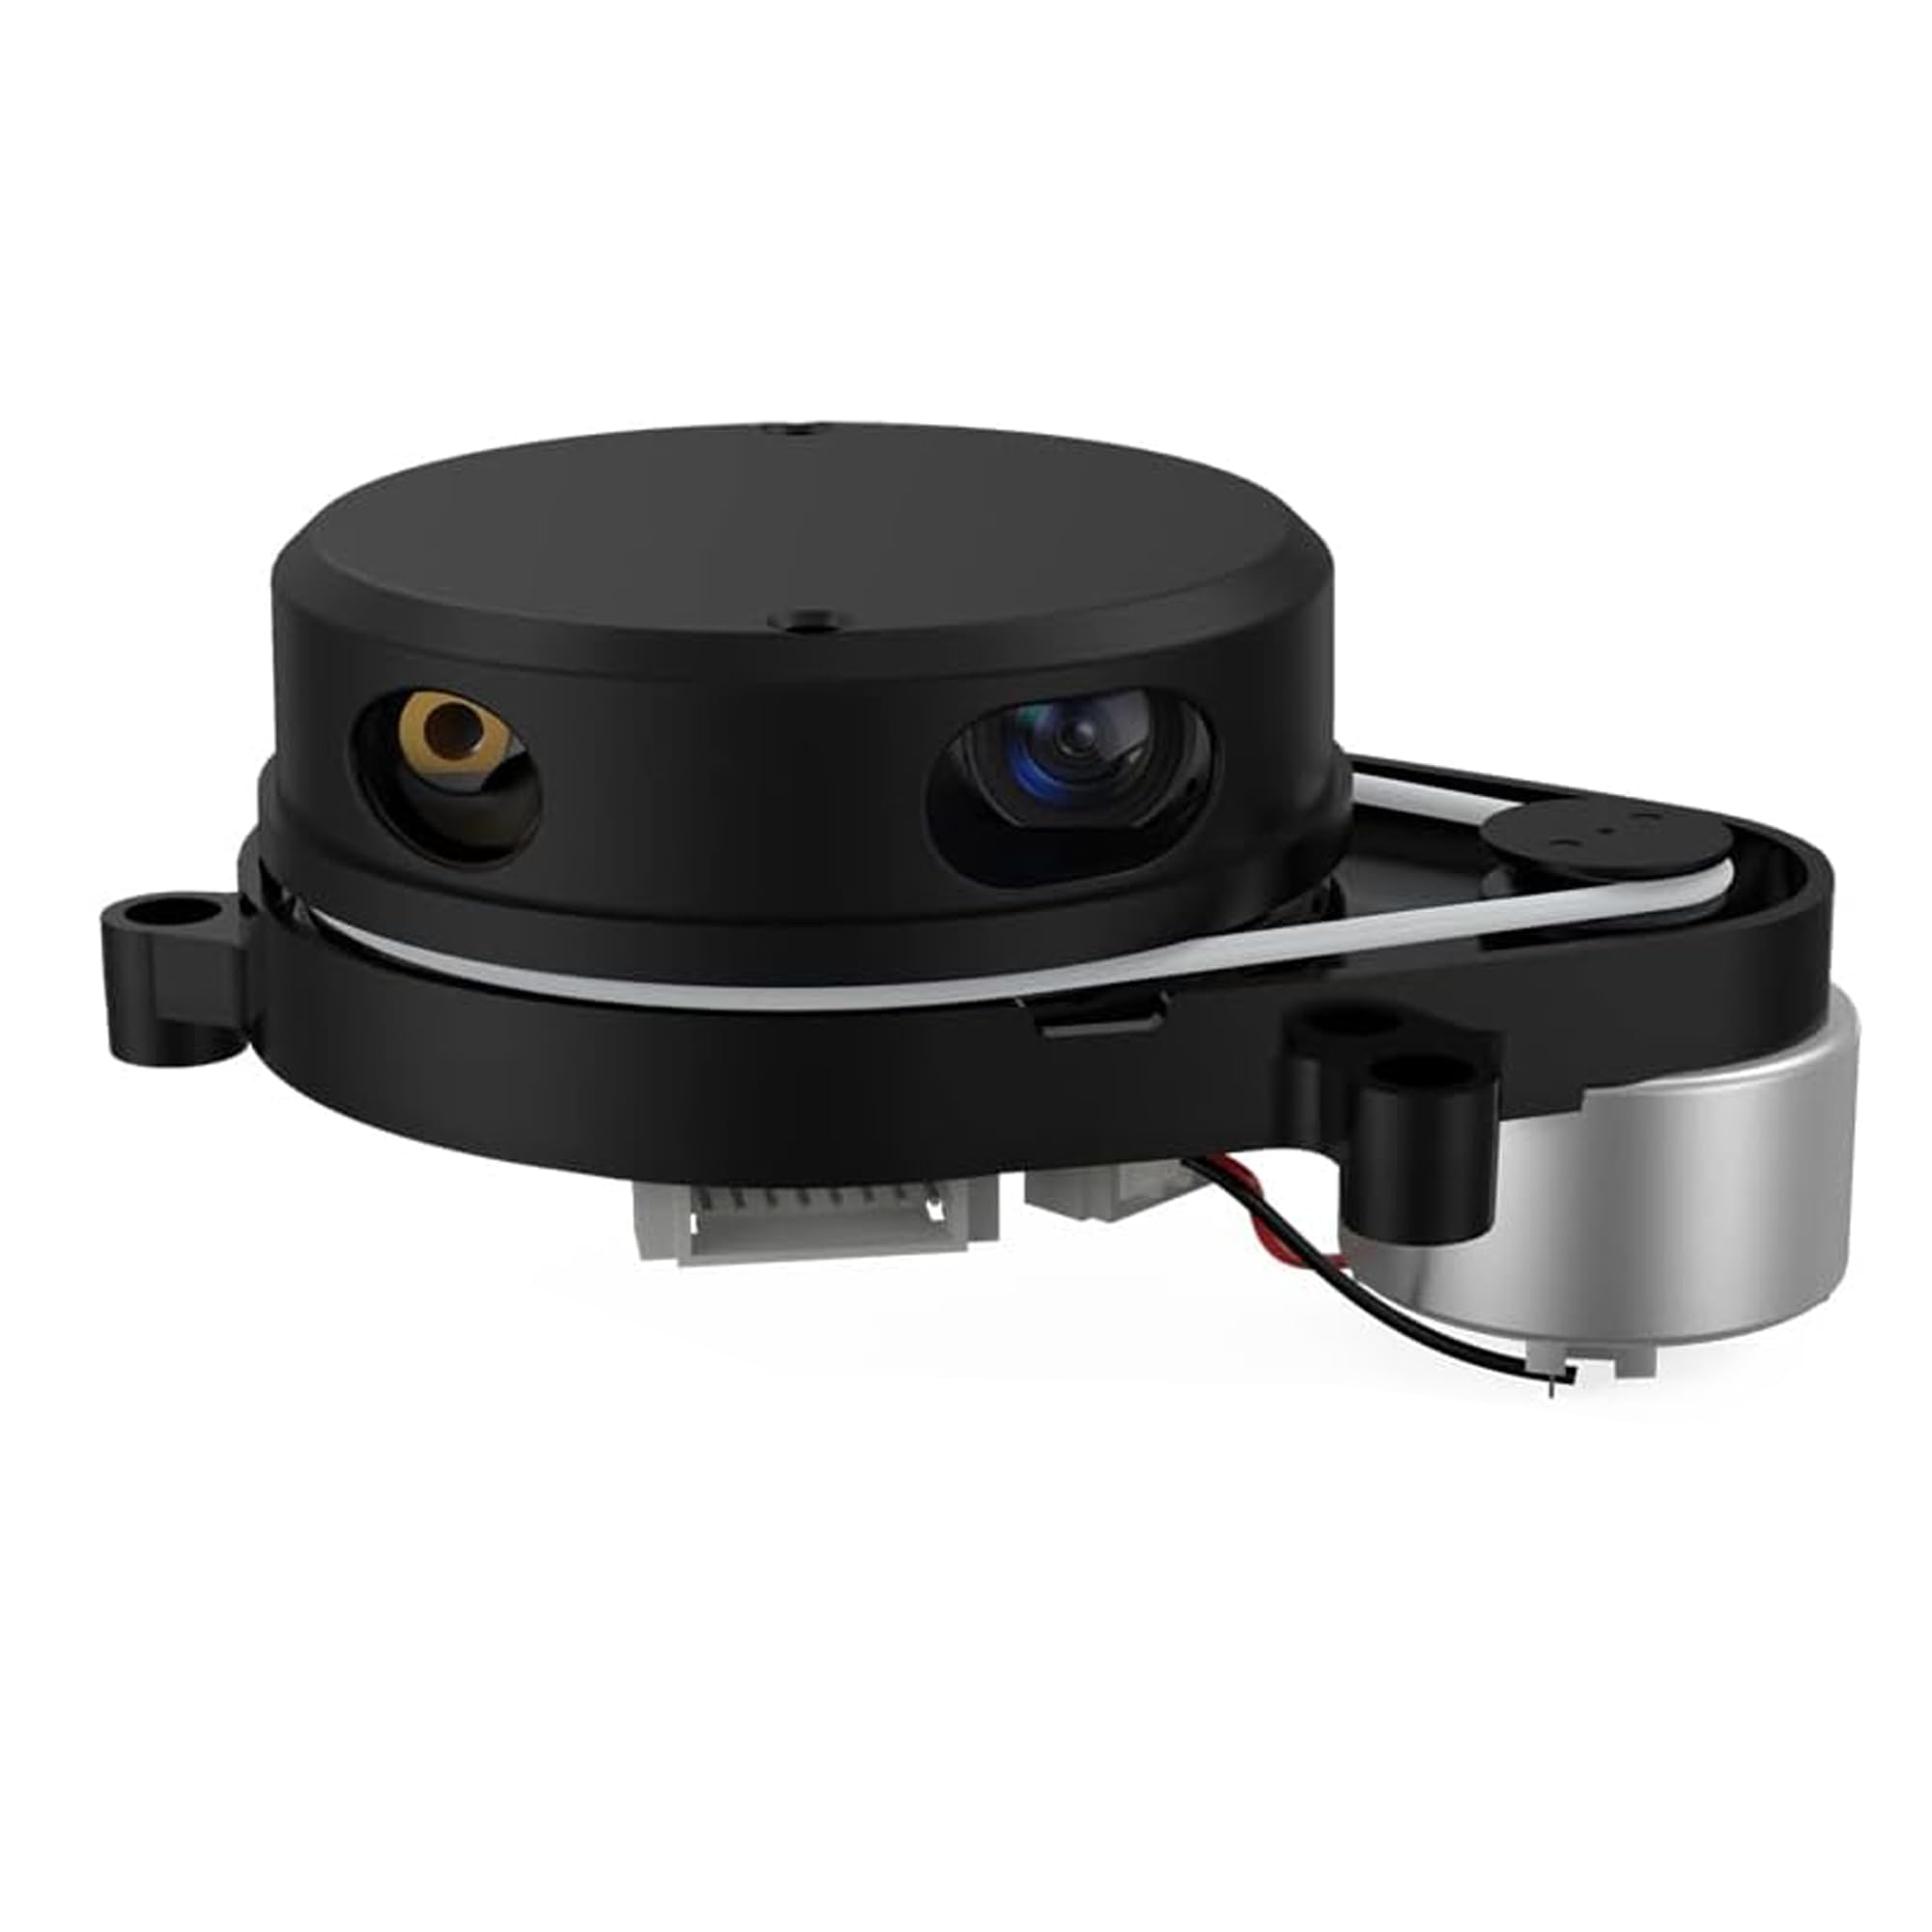
\includegraphics[width=0.5\textwidth]{img/lidar.jpg}
    \caption{The YD-LiDAR X4 Pro.}
    \label{fig:X4_PRO} 
\end{figure}

Because the LiDAR only outputs the point cloud data, and we need to find the color of the pillars as well, a wide FOV camera is used in tandem. It is only used to determine the color of the pillar and not used for detection. The LiDAR detects the pillar and the image from the camera is then used to assign the color. This keeps the compute costs very low and allows for very fast inference. The camera used is the \textbf{Arducam IMX219 Wide Angle Camera}. It has a field of view of $175^\circ$. This allows us to have the maximum window for inference possible as we don't need the data resolution a camera based solution would.

\begin{figure}[H]
    \centering
    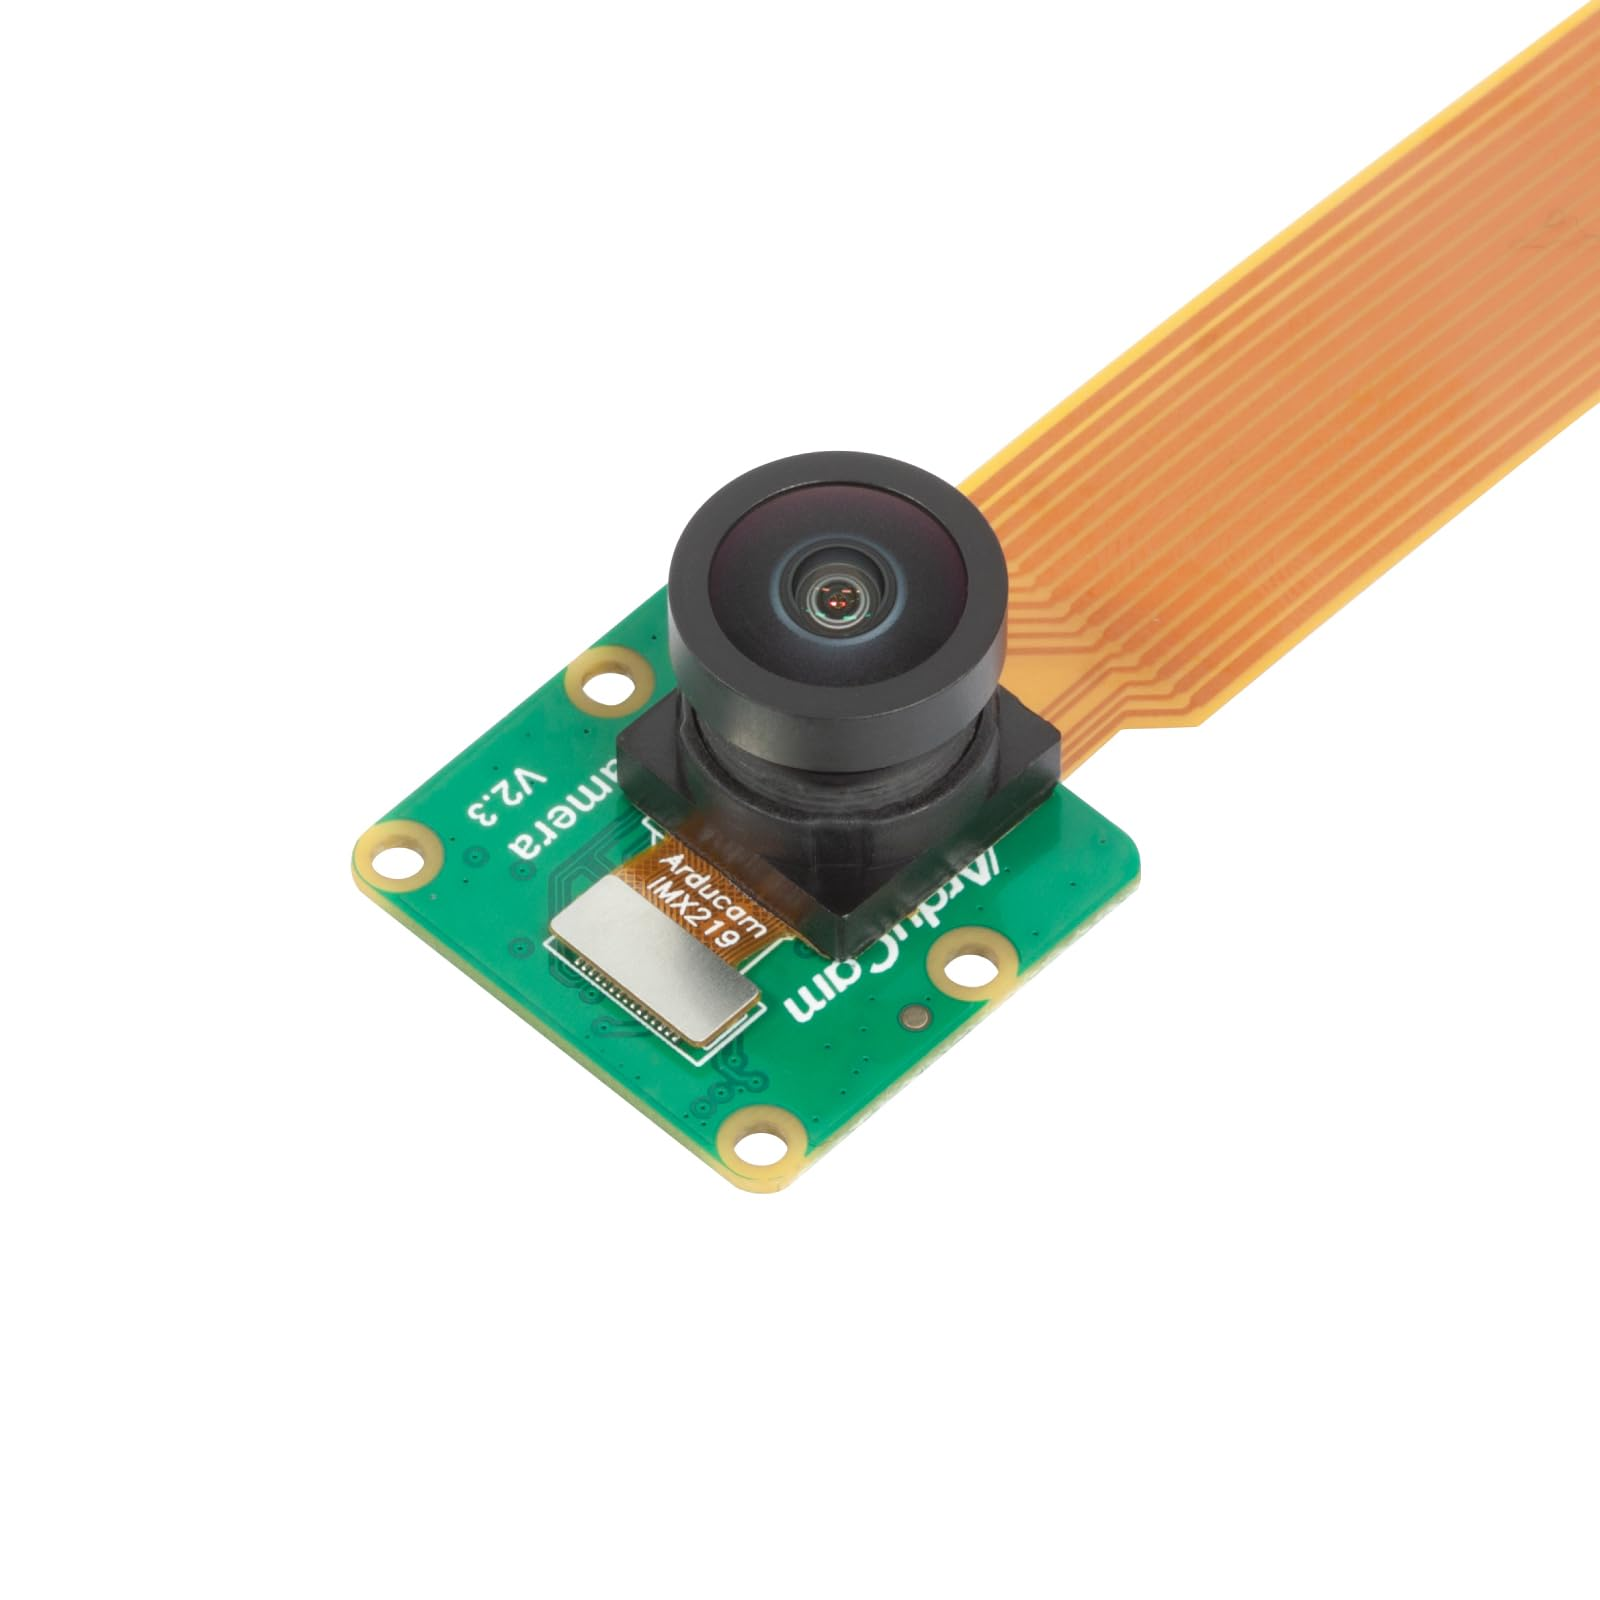
\includegraphics[width=0.5\textwidth]{img/camera.jpg}
    \caption{The IMX219 with a very wide angle lens.}
    \label{fig:Cam} 
\end{figure}

\subsection{Compute}

The compute module doesn't need to be something excessive like the Jetson Orion Nano. The compute required to complete both the challenges is fairly low and could be done on an STM32 H7 micro-controller as well. The compute module has to fulfill the following requirements:

\begin{enumerate}
\item Small form factor.
\item Have a USB poet.
\item Have a Camera Serial Interface .
\item Run ROS or Micro ROS.
\item Have a decent number of exposed IO pins for accessories.
\item Have the ability to read/write code for easy iterations.
\end{enumerate}

This led to the Raspberry Pi 4B. Any other similar Single Board Computer (SBC) can be used. The 4GB RAM version was chosen so that a graphical user interface could be ran on it if needed when editing code during the competition. It would also provide sufficient headroom. A 2GB RAM version would have also been sufficient. A Raspberry Pi 5 would be overkill. The Pi 4 is also cheaper and easier to source. It would also have the compute needed to run the control loop at higher frequencies and have faster and more accurate control. \\

The only downside of the Rspberry Pi was it's size. It's a lot larger than needed, and occupies crucial space in the limited volume. This was solved with intentional and clever design. It's availability of USB ports and the CSI makes it a very appealing solution. Custom hardware, ST based micro-controller or a board with the Raspberry Pi Compute Module, can be used but would be harder to source and would involve a longer development time. The Raspberry Pi also acts as a drop in solution as it has an external micro-SD card where all the code is stored, allowing for easy access and replaceability.

\begin{figure}[H]
    \centering
    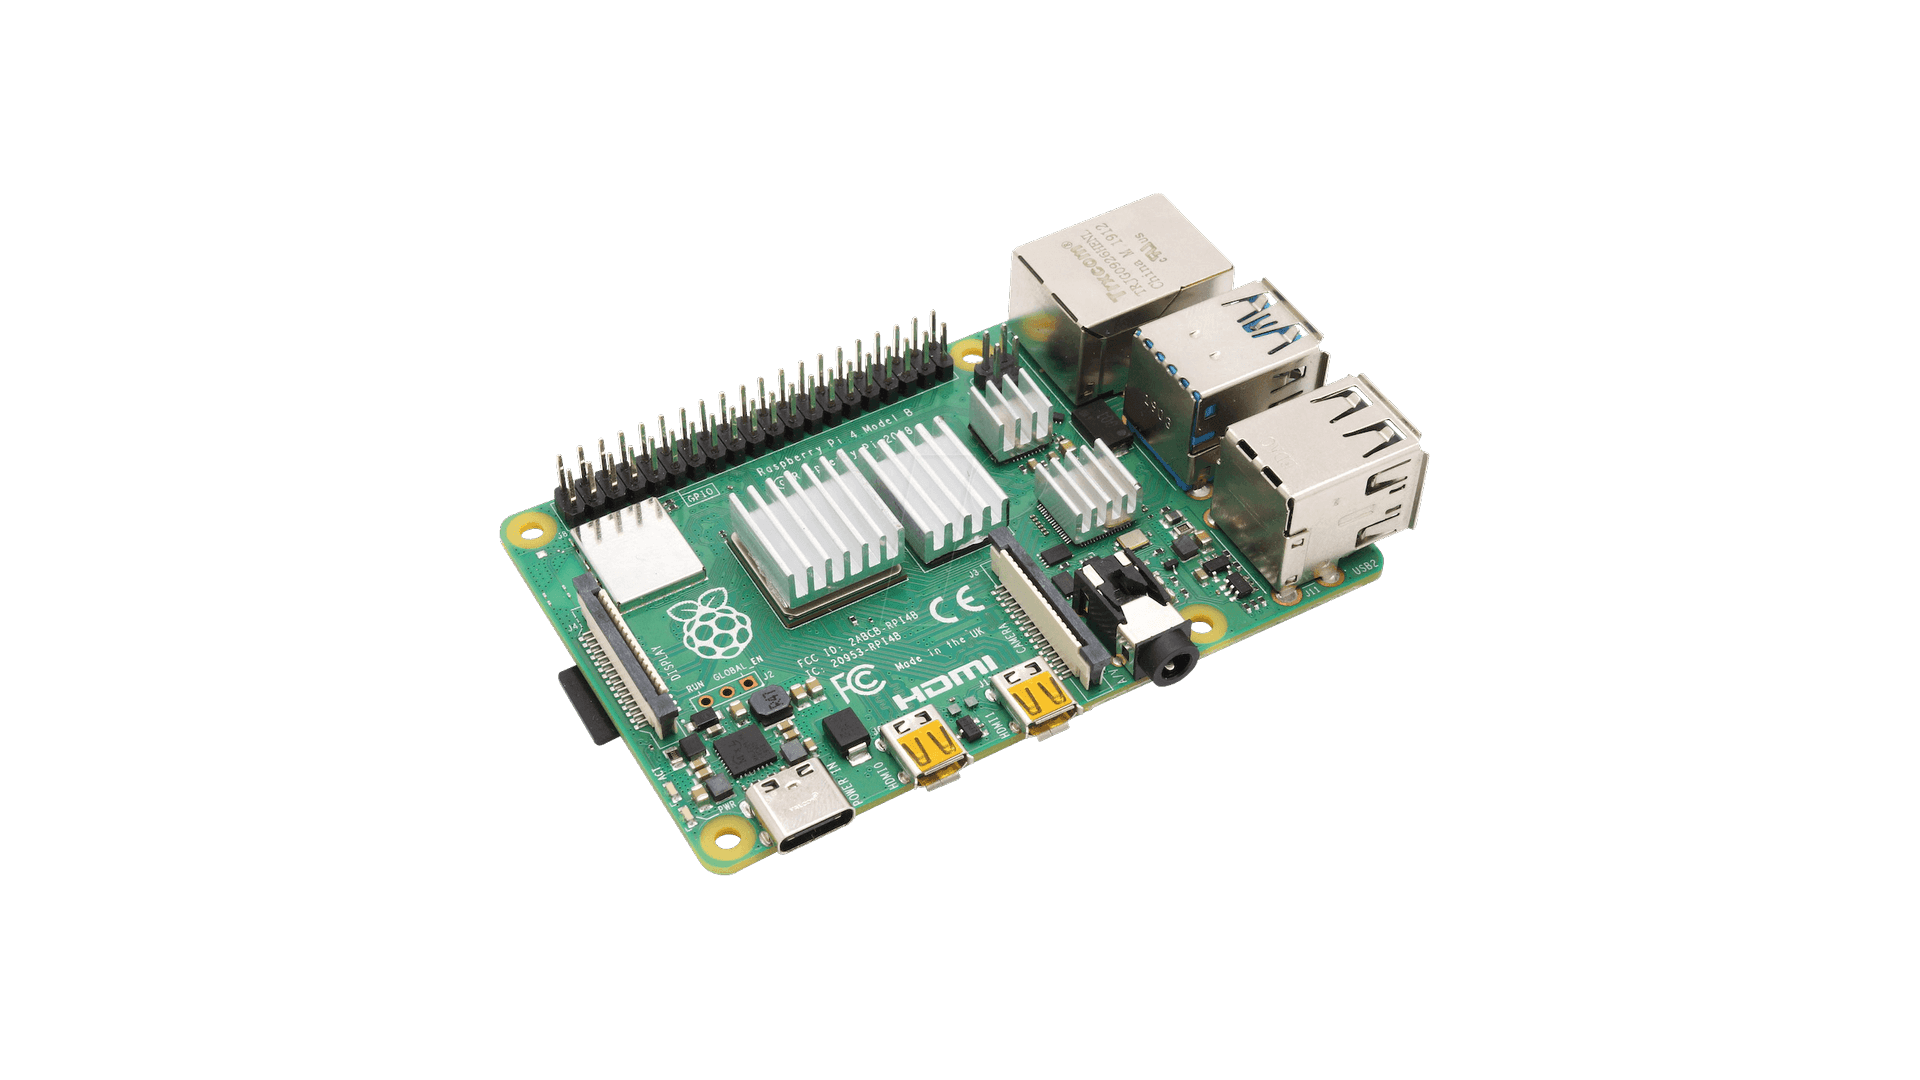
\includegraphics[width=.8\textwidth]{img/rpi4b.png}
    \caption{The Raspberry Pi 4 Model B.}
    \label{fig:Rpi} 
\end{figure}

\subsection{Motion}

A \textbf{rear wheel drive system} was chosen as it would distribute the complexity of the steering and drive systems, allowing easier manufacturing and assembly. The trade-off made here was that a \textbf{differential would be required} to prevent under steer that would be cause when turning at tight radii and slow speeds. This increases the complexity slightly, but not as much as using a drive and steering would need. \\

The motion system can be broken down into two parts, the drive system and the steering system. \\

\subsubsection{Drive System}

A brush less DC (BLDC) motor is proffered over a brushed motor due to it's higher resolution of speed changes particularly at a low speeds. That comes particularly handy when parallel parking. It is also preferred due to its efficiency and torque. The ideal case would be a stepper or BLDC motor with Field Oriented Control (FOC) as it would provide excellent position and torque control, but sourcing such FOC motor drivers in a small and compact size is very hard and expensive. A note should be made that developing such a custom FOC motor driver for 10-20A should not be hard but would take time. \\

For the motor, a Surpass Hobby \textbf{36 mm diameter in runner BLDC motor} is used. The 36 mm diameter is chosen as it provides enough \textbf{torque, acceleration and internal breaking} for a 1.5 kg vehicle. The length of the motor is 74 mm. This makes it a \textbf{3674 motor}. The motor is also widely used in scale RC cars and hence is easy to source. The motor is rated at \textbf{1700 kv}, which provides generous speed and high torque. \\

\begin{figure}[H]
    \centering
    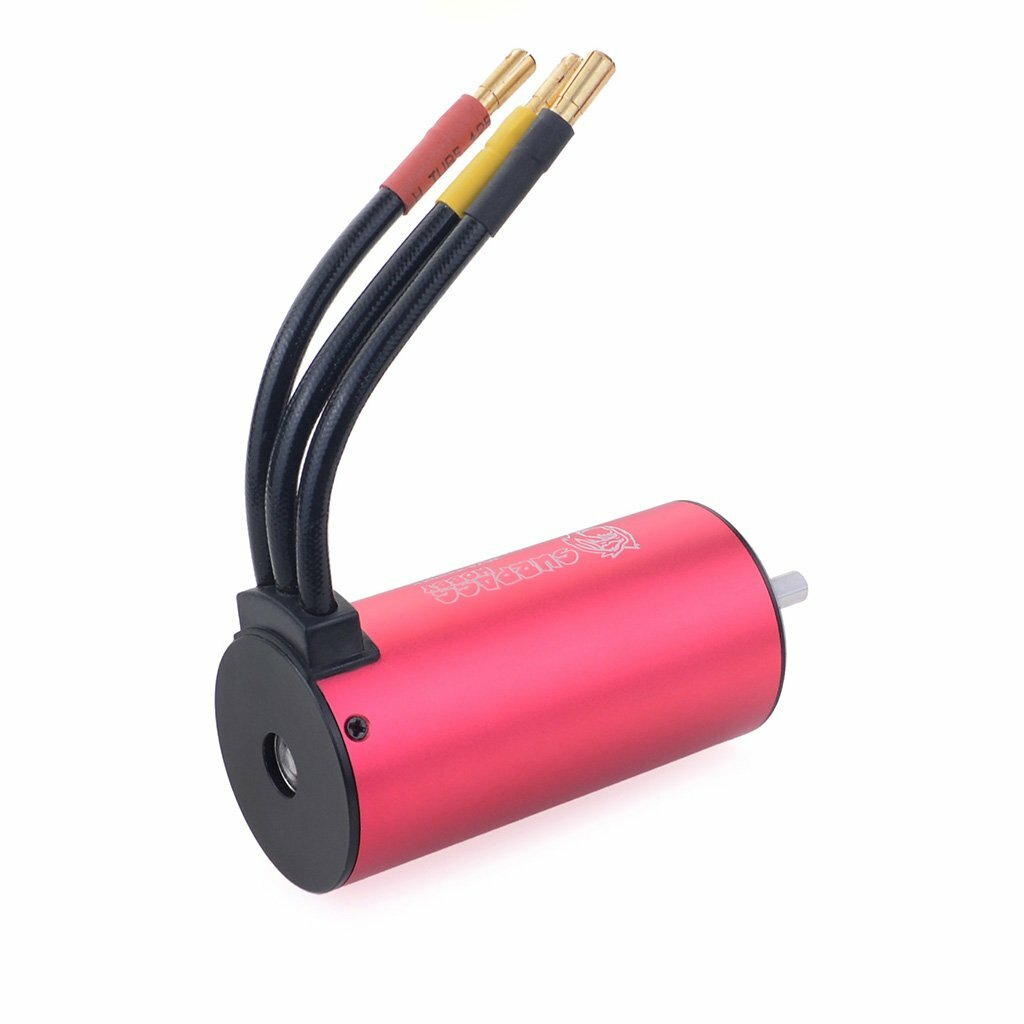
\includegraphics[width=.5\textwidth]{img/motor.jpg}
    \caption{The Motor.}
    \label{fig:motor} 
\end{figure}

A Surpass Hobby 3 Phase \textbf{120A 4S ESC} is used. This Electronic Speed Controller is preferred due to its high \textbf{reliability and headroom, along with its configurability}. The ESC can be configured to operate at certain speed, torque and braking levels with a configurator device. \\

\begin{figure}[H]
    \centering
    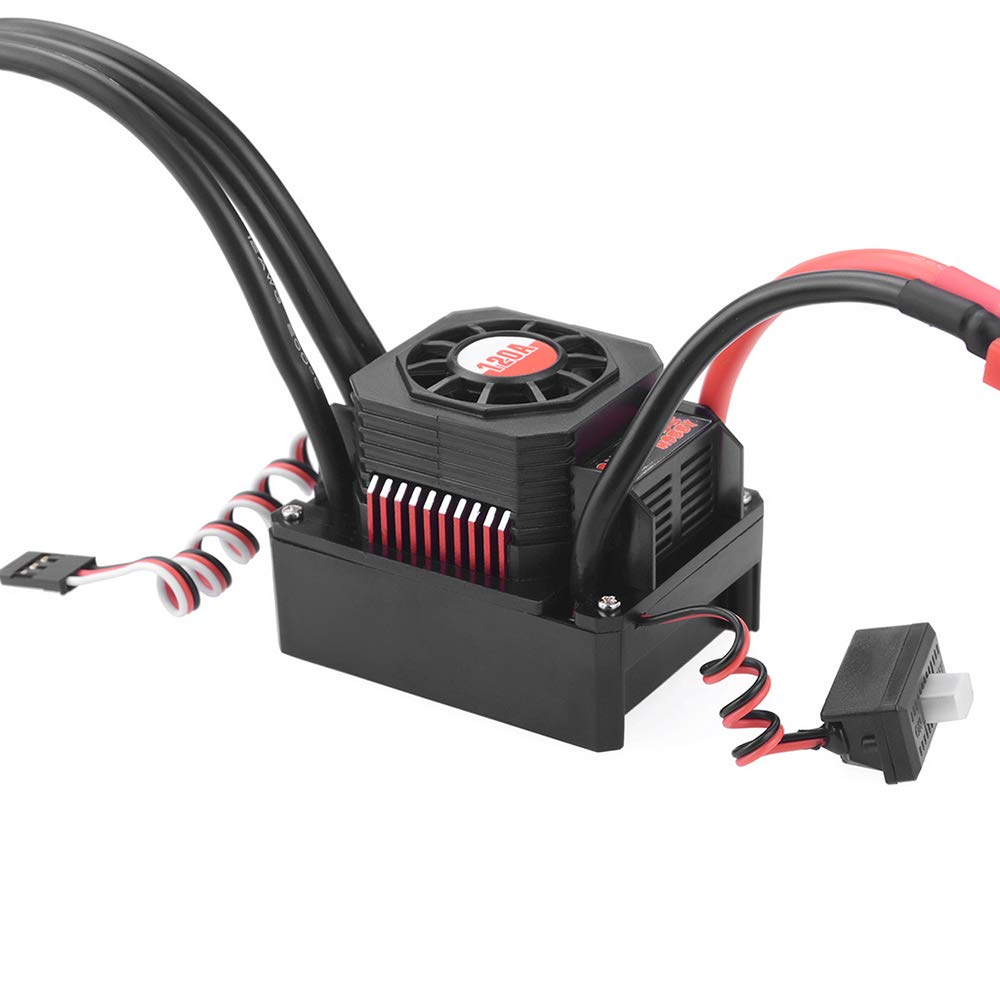
\includegraphics[width=.5\textwidth]{img/esc.jpg}
    \caption{The ESC.}
    \label{fig:ESC} 
\end{figure}

Do note that if built again, a shorter motor and lower ampere rated ESC would be used, something like a 3650 motor and a 60A ESC. The 3674 motor is too long and has excessive torque that is not really needed. The shorter motor should be used to reduce the weight as much as possible. The ideal motor would be a 3650 motor rated somewhere about 1000 kv. The 60A ESC would also be chosen to reduce weight. The current setup was chosen because it is what was available without purchasing new components. \\

\begin{figure}[H]
    \centering
    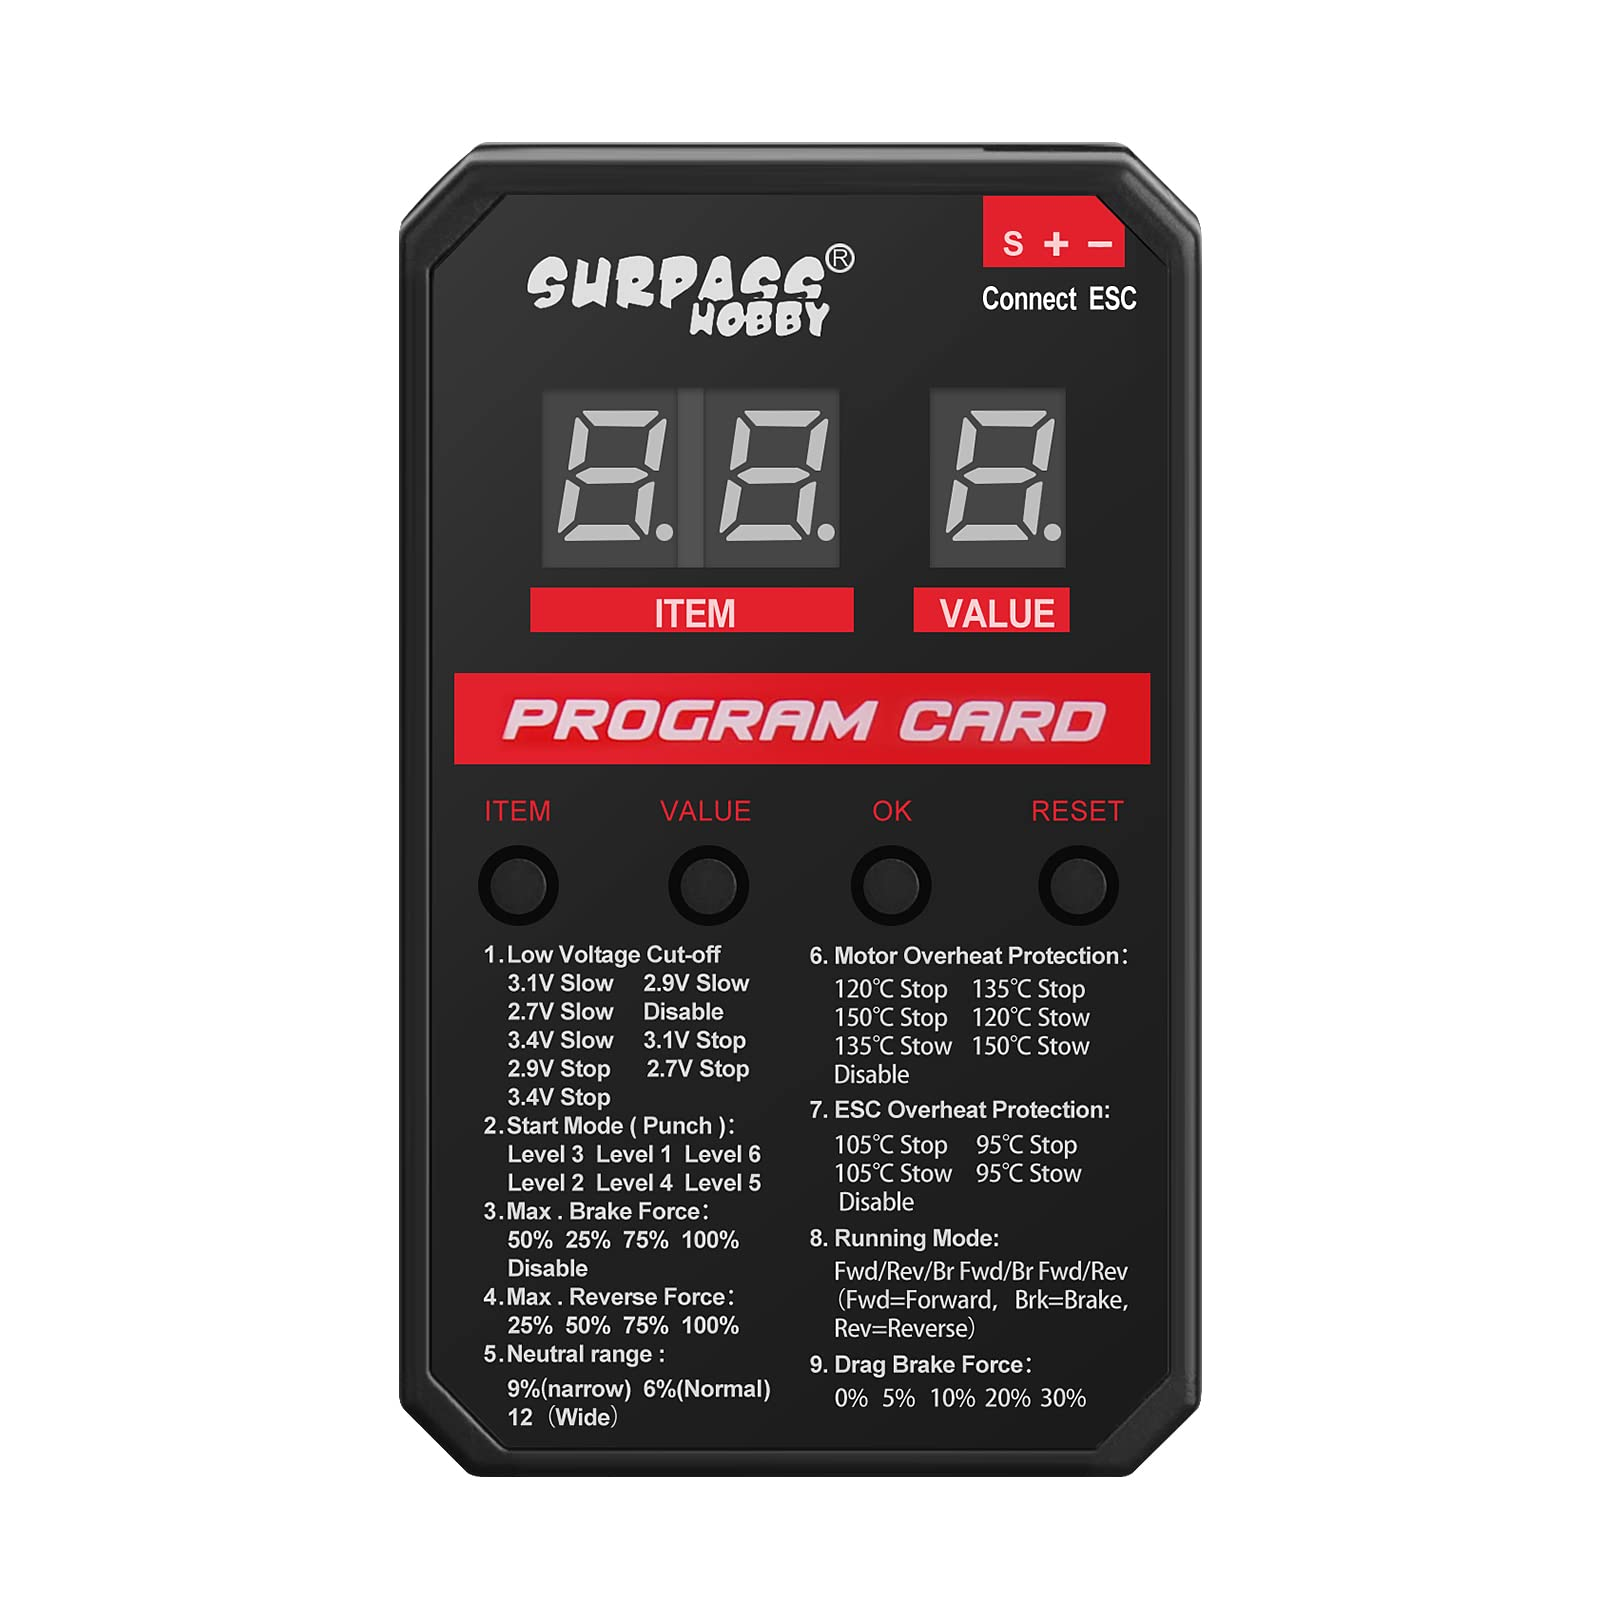
\includegraphics[width=.3\textwidth]{img/configurator.jpg}
    \caption{The Configuration Device that connects via PWM.}
    \label{fig:configurator} 
\end{figure}

\subsubsection{Steering System}

A \textbf{direct drive steering system} was chosen for the vehicle, meaning that the servo directly drives the wheels. This was chosen as the steering links would be manufactured using 3D printing and each joint would cause additional backlash in the linkage mechanism. A system with a grater mechanical leverage would hence be more complex and less accurate, while taking more volume. \\

The \textbf{S2500M} servo motor is used, which provides a torque of about 25 $\frac{kg}{cm}$ at about $8$V. This would be provide ample headroom in a direct drive steering system. The only downside to contend with in this system is its weight and the fact that the servo runs on $8$V, meaning it will need its own power supply. Do note that a lower torque servo that operates on $5$V can be used if needed, the S2500M was available without purchasing new components. \\

\begin{figure}[H]
    \centering
    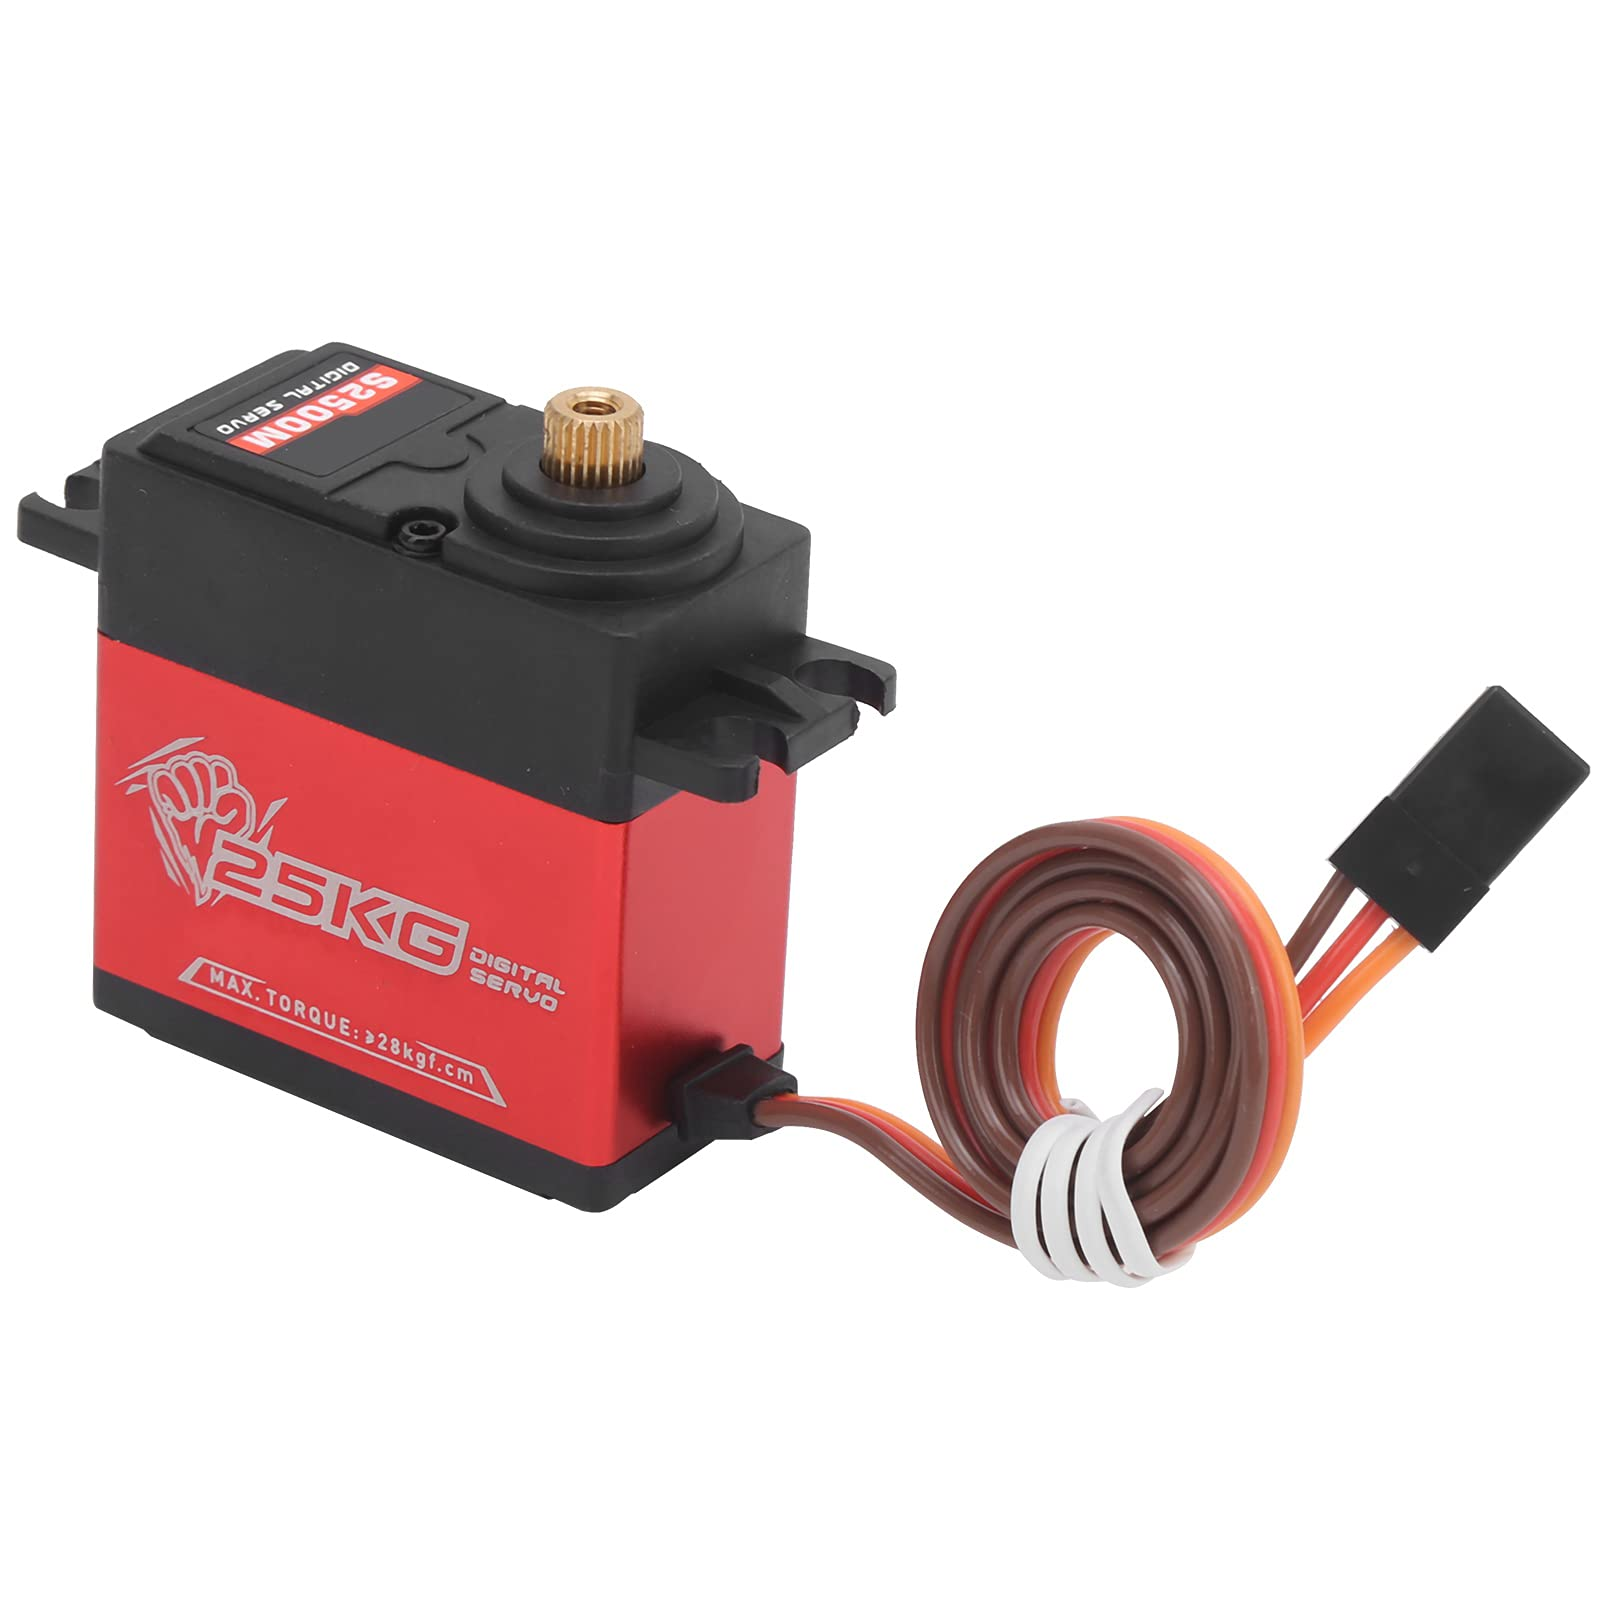
\includegraphics[width=.5\textwidth]{img/servo.jpg}
    \caption{The S2500M metal gear servo motor.}
    \label{fig:servo} 
\end{figure}

\subsection{Power Management}

The batteries were chosen on strict power consumption metrics. \\

\begin{table}[htbp]
\centering
\small
\caption{System Power Usage and Electrical Specifications}
\label{tab:power_usage}
\begin{tabularx}{\textwidth}{>{\raggedright\arraybackslash}X >{\raggedright\arraybackslash}p{2.2cm} >{\raggedright\arraybackslash}p{1.8cm} >{\raggedright\arraybackslash}p{2.2cm} >{\raggedright\arraybackslash}p{2.2cm} >{\raggedright\arraybackslash}X}
\toprule
\textbf{Component} & \textbf{Voltage Rail} & \textbf{Idle Current} & \textbf{Typical Draw} & \textbf{Peak Draw} & \textbf{Power Regulator / Impact} \\
\midrule
Raspberry Pi 4B (4GB) & 5.15V DC & 600 mA (3.1 W) & 1.2A--1.5A (6.2--7.7 W) & 2.2A--2.5A (11.3--12.9 W) & TI LM61460 (5.15V Buck); Primary SBC running ROS, vision, and control loops. \\
YD-LiDAR X4 Pro & 5.0V / 5.15V DC & 280 mA (1.4 W) & 330--380 mA (1.7--1.95 W) & 800--1000 mA (4.0--5.0 W) & 5.15V Rail; 360$^\circ$ 2D LiDAR for mapping, wall-following, and parking. \\
Arducam IMX219 & 3.3V / 5.0V DC & 100 mA (0.5 W) & 150--200 mA (0.75--1.0 W) & 300 mA (1.5 W) & RPi CSI Bus; 175$^\circ$ Ultra-Wide FOV camera for pillar color classification. \\
Surpass Hobby 3674 Motor & 14.8V--16.8V DC & 2.6A--3.1A (38.5--46 W) & 4.0A--7.0A (60--105 W) & 15A--25A (220--370 W) & Direct 4S LiPo; 1700KV BLDC rear drivetrain propulsion motor. \\
Surpass Hobby 120A ESC & 14.8V--16.8V DC & 100 mA (1.5 W) & 100--200 mA (1.5--3.0 W) & 120A Cont. / 760A Burst & Direct 4S LiPo; 3-Phase electronic speed controller with PWM interface. \\
S2500M Servo Motor & 8.0V DC & 100 mA (0.8 W) & 500mA--1.0A (4.0--8.0 W) & 1.8A--2.0A (14.4--16.0 W) & TI TPS62932 (8V Buck); 25 kg$\cdot$cm high-voltage metal gear steering servo. \\
Peripherals \& PCB Logic & 5.15V / 8.0V DC & 20 mA (0.1 W) & 50--100 mA (0.25--0.5 W) & 150 mA (0.75 W) & PCB Hat; Onboard status LEDs, switches, and ToF headers. \\
\midrule
\textbf{Total 5.15V Rail} & \textbf{5.15V DC} & \textbf{~1.0 A (5.15 W)} & \textbf{~1.8A--2.1A (9.3--10.8 W)} & \textbf{~3.5A--3.8A (18.0--19.6 W)} & Regulated by TI LM61460 (6A Cont. Limit). \\
\textbf{Total 8.0V Rail} & \textbf{8.0V DC} & \textbf{~0.1 A (0.8 W)} & \textbf{~0.5A--1.0A (4.0--8.0 W)} & \textbf{~1.8A--2.0A (14.4--16.0 W)} & Regulated by TI TPS62932 (2A Cont. Limit). \\
\textbf{Total System Draw} & \textbf{14.8V Nominal} & \textbf{~0.8 A (12 W)} & \textbf{~5.5A--8.5A (80--125 W)} & \textbf{~18A--28A (260--410 W)} & \textbf{2x DOGCOM 4S 850 mAh} (1700 mAh Total). \\
\bottomrule
\end{tabularx}
\end{table}

To provide adequate headroom for the 3+ minutes of operation needed, \textbf{2 DOGCOM 4S 850 mAh batteries were used in parallel}. A single 4S 850 mAh battery in testing at full motion capabilities provided power for about 2.5 minutes before it went below the safe discharge voltage of 3.5 V per cell. Hence a second battery is needed for headroom. \\

The 4S batteries are used as they have the maximum voltage compatible with the setup, allowing the maximum acceleration and torque for the vehicle. The batteries use a \textbf{Li-Po (Lithium Polymer)} chemistry as that provides the high discharge current needed. It is also widely available and hence easy to source. On a larger scale vehicle, Li-Ion cells would be used due to their longer discharge cycle rating as the only major draw back with Li-Po batteries are their lower charge cycle rating. \\

\begin{figure}[H]
    \centering
    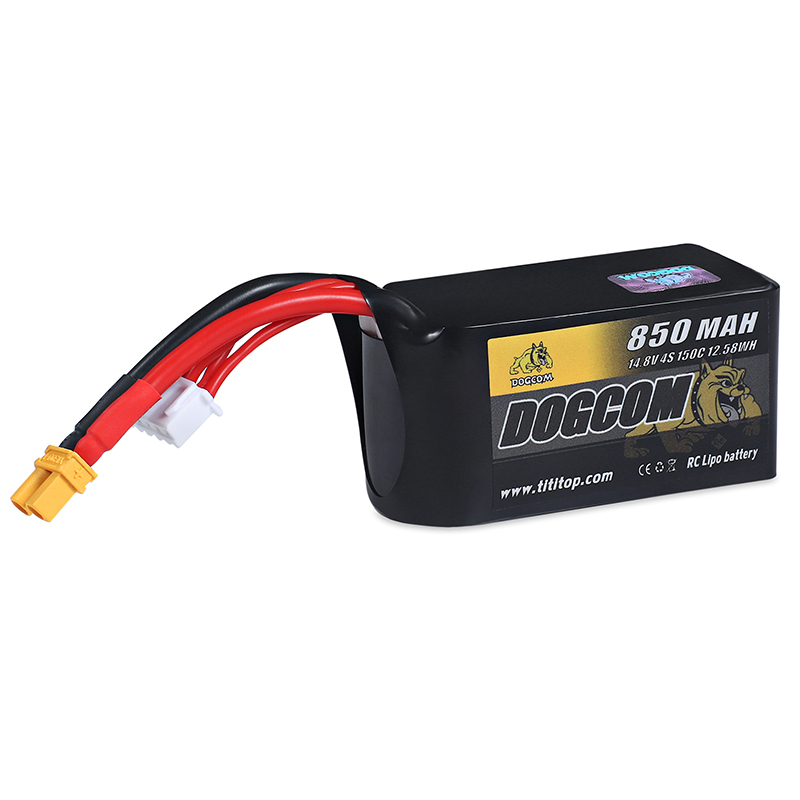
\includegraphics[width=.5\textwidth]{img/battery.jpg}
    \caption{The DOGCOM 4s 850 mAh battery.}
    \label{fig:battery} 
\end{figure}

\subsection{The Additional Hardware}

Additional hardware such as bearings and wheels are needed to build the vehicle. These are things that cannot be 3D printed and are manufactured in other ways or are sourced. \\

\subsubsection{Bearings}

For the two front steering knuckles, a \textbf{thrust roller bearing} is used. This is a type of bearing that combines a needle and thrust bearing in a single housing. It is used to constraint the location of the two front steering wheels though the axis of rotation and ensure there is no play present. If a normal roller ball bearing would be used, the outward and asymmetric torque of the wheel "pin" would misalign the groove and the balls causing excessive play. The thrust roller bearing is a compact solution used in real cars as well. \\

The inner diameter of the bearing is 12 mm. It is the "\textbf{BCWN-T-d12-IR}" bearing, sourced from JLCMC. \\

\begin{figure}[H]
    \centering
    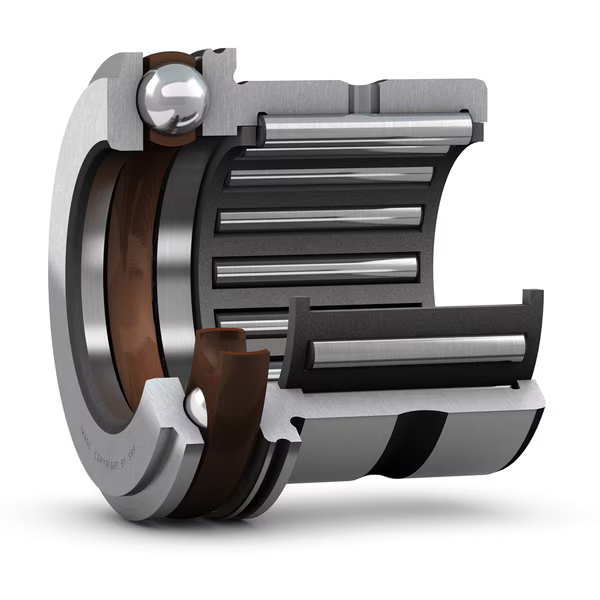
\includegraphics[width=.5\textwidth]{img/needle_roller.png}
    \caption{The internals of a Combined needle roller / thrust ball bearing.}
    \label{fig:needle_roller_thrust_bearing} 
\end{figure}

For the differential, traditional roller ball bearings were used as the axial forces transferred are not that high. The \textbf{6901ZZ} ball bearing is used as it is in a very compact package that has an internal diameter of 12 mm, an external diameter of 24 mm and a width of 6 mm, making it ideal to put in the already compact differential gear box. \\

\begin{figure}[H]
    \centering
    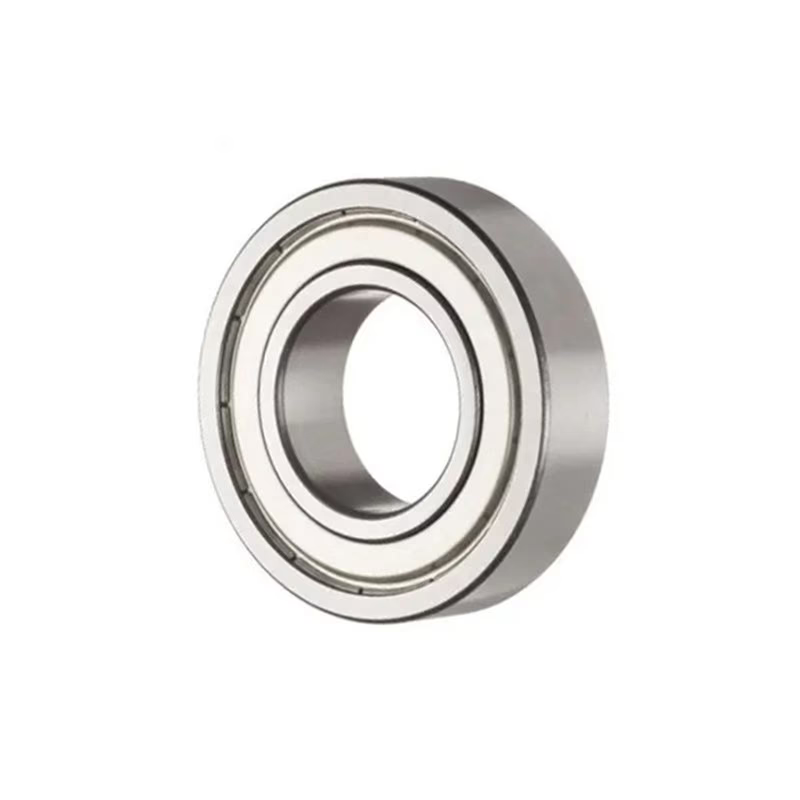
\includegraphics[width=.5\textwidth]{img/roller.png}
    \caption{The 6901ZZ roller ball bearing.}
    \label{fig:roller_bearing} 
\end{figure}
 
To support the rear axle, needle roller bearings are used. They are used as they have low friction and can withstand very high forces perpendicular to the axis of rotation, prefect for transferring the weight from the main body of the vehicle to the wheels. The "\textbf{BCWG-NK12/12}" bearing was used, sourced from JLCMC. It has an inner diameter of 12 mm, an outer diameter of 19.5 mm and is 12 mm deep. \\

\begin{figure}[H]
    \centering
    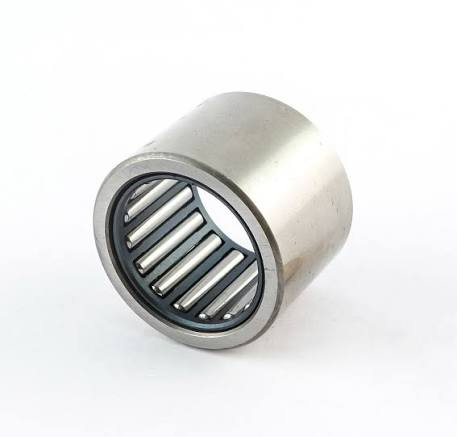
\includegraphics[width=.5\textwidth]{img/needle_roller.jpeg}
    \caption{The Needle Roller bearing.}
    \label{fig:needle_roller_bearing} 
\end{figure}

\subsubsection{Carbon Fiber Tubes}

Carbon fiber tubes were used at several places as axles, linkage connectors and structural connectors. This decision was made as carbon fiber has a very high tensile strength and is particularly very stiff perpendicular to it's length. \\

A combination of 2 diameters were used. The axle for the rear two wheels were made using \textbf{12 mm outer diameter} and 10 mm inner diameter carbon fiber tubes. Any aluminum or steel shaft could be used here, but a 3D printed shaft cannot be used as the layer lines of the print would be perpendicular to the layer lines, leading to very weak prints. Carbon fiber was used as it is light weight and relatively easy to source in \textbf{roll wrapped rods}. This tube consists of "twill" and not "toe". \\

\begin{figure}[H]
    \centering
    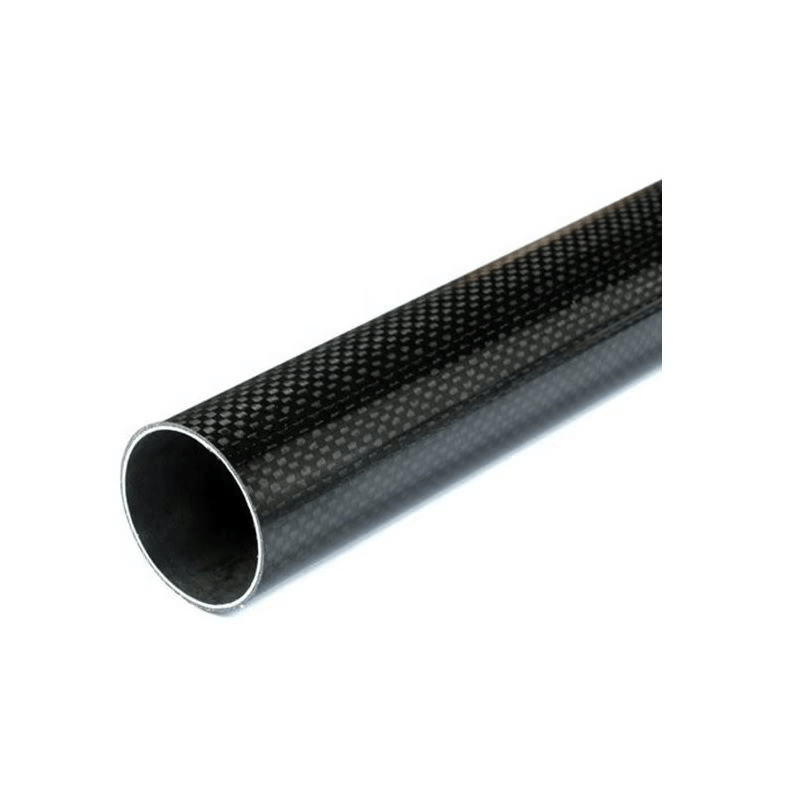
\includegraphics[width=.5\textwidth]{img/12cf.png}
    \caption{The 12 mm CF rod.}
    \label{fig:12mm_cf} 
\end{figure}

The other rod used was a \textbf{3 mm outer diameter solid pultruded} rod. It is used in the steering links as well as the structural spin that runs throughout the vehicle to provide stiffness to the frame and not let the printed parts sag. It is pultruded, meaning it does not consist of carbon fibers but of chopped carbon bits held by epoxy. It is comparatively less stiff but still very strong. It consists of "toe" and no "twill". \\

\begin{figure}[H]
    \centering
    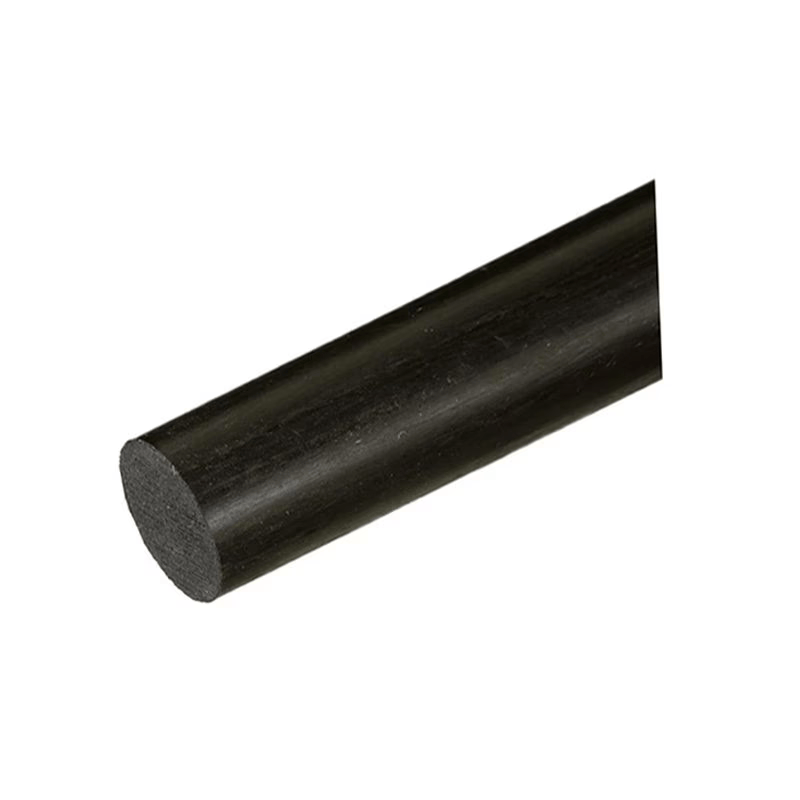
\includegraphics[width=.5\textwidth]{img/3cf.png}
    \caption{The 3 mm PultrudedCF rod.}
    \label{fig:3mm_cf} 
\end{figure}

\subsection{Wheels}

\subsubsection*{Design Constraints \& Diameter Selection}
The selection of the wheel diameter is one of the most critical foundational decisions in the vehicle's architecture, as it directly locks in ground clearance, overall vehicle height, wheelbase geometry, and internal volume distribution. \\

Two strict physical constraints dictated the wheel sizing. First, the maximum overall height of the vehicle had to remain strictly under $80\,\text{mm}$ to ensure the YD-LiDAR X4 Pro maintains an unobstructed $360^\circ$ laser line sweep at a height of $90\,\text{mm}$, which is well clear of the $100\,\text{mm}$ arena perimeter walls. Second, the ground clearance had to accommodate the Surpass Hobby 3674 rear drive motor, which has an outer diameter of $36\,\text{mm}$. To prevent the motor housing from dragging against flat ground without suspension, the wheel diameter had to comfortably exceed $36\,\text{mm}$. \\

In previous competition iterations, $65\,\text{mm}$ wheels were utilized. However, they proved excessively large, creating severe vertical congestion between the drive motor, chassis braces, and LiDAR platform. Consequently, a target wheel diameter of $\approx 50\,\text{mm}$ ($48$--$50\,\text{mm}$) was selected, offering adequate ground clearance for the $36\,\text{mm}$ motor while maintaining a compact vertical profile. \\

\subsubsection*{Commercial Evaluation \& Shore Hardness Selection}
Commercially available $2$-inch ($48\,\text{mm}$) FingerTech Combat Robot wheels were initially evaluated due to their high-traction tread and $40\text{A}$ durometer rating. \\

The durometer rating measures an elastomer's resistance to indentation on the Shore A scale, where lower values ($20\text{A}$--$30\text{A}$) indicate soft, gel-like compounds, and higher values ($70\text{A}$--$90\text{A}$) represent rigid plastics. A hardness of \textbf{40\text{A} Shore Hardness} represents the optimal balance for autonomous racing, providing exceptional surface traction and grip on the track mat without disintegrating or tearing under high motor acceleration torque. \\

Because $2$-inch $40\text{A}$ combat wheels were unavailable domestically in India and prohibitively expensive to import, a custom in-house casting process was developed instead. 

\subsubsection*{Manufacturing \& Polyurethane Casting Procedure}
To fabricate custom $48\,\text{mm}$ high-traction tires, a two-part casting process was established using SLA resin 3D-printed molds and PLA wheel hubs. The Polyurethane selected was a 2 part 10:4 ratio 40A mixture made by Aditya Silicone. Standard teflon based mold release spray was used. \textit{Please ensure proper PPE and safety when working with these materials.} \\

For the core wheel hub fabrication (\texttt{Wheel Hub.step}, see Figure \ref{fig:C_W_H}), the part is 3D printed in PLA with an $18\,\text{mm}$ width. To ensure a permanent mechanical bond between the printed hub and the cast tire, the outer cylindrical contact surface is printed with a "Fuzzy Skin" texture ($0.1\,\text{mm}$ thickness, $0.2\,\text{mm}$ density), creating microscopic interlocks for the curing compound. \\

For the precision mold fabrication (\texttt{Tools/Tire Mold.step}, see Figure \ref{fig:C_W_Mold}), a two-part split mold was 3D printed using Stereolithography (SLA) resin. SLA resin was selected over FDM because its smooth surface finish eliminates layer lines, allowing clean demolding without requiring draft angles. The mold halves clamp together using four $\text{M3} \times 30\,\text{mm}$ screws, washers, and $\text{M3}$ hex nuts. \\

During the polyurethane casting phase, a two-part liquid Polyurethane elastomer formulated to $40\text{A}$ Shore hardness is mixed, degassed to remove air bubbles, and poured through the mold's entry port until liquid emerges from the riser exit port. After a $24$-hour cure cycle, the mold is unbolted, producing a balanced, high-traction polyurethane tire bonded securely to the PLA wheel hub. \\

A file called \texttt{Castings.csv} contains all the details of each and every individual castings, including Part A and Part B ratios, weights and remarks. It can be found in the \texttt{Other} folder.

\pagebreak

\section{PCB Assembly}

The first question one should ask is why use a PCB at all? Why not just use jumper wires and other modules? \\

The answer is quite simple yet complex. A Printed Circuit Board (PCB) integrates all the power management components needed into a sleek and compact form factor without a lot of wiring. The Raspberry pi has a $20 \times 2$ pin interface, which isn't very neat in it self. One can connect the individual jumpers to the header pins but it becomes VERY cumbersome very fast. Hence a PCB is almost necessary for a vehicle that can be easily serviced and is well engineered. Another major driver for this, as you will learn, comes from issues learnt from Siddesh's participation in WRO the previous year. KiCAD was used as the eCAD tool to design the PCBs.\\

\subsection{Purpose}

When participating in WRO 2025, the SD Card we were using failed on us the day before the final competition. It was corrupted and the Raspberry Pi would not boot up at all. Turns out the issue was that that the Raspberry Pi was constantly undervolting under load. We had attempted to add a capacitor before the competition to resolve the issue, but the effort proved futile. Upon reviewing the logs, we confirmed that these undervoltage events were, in fact, what caused the SD card to fail. The buck converter was rated for $5$V at a nominal current of $3$A and a burst current of $5$A. Yet the Raspberry Pi wouldn't boot. \\

The Raspberry Pi needs a voltage higher that just $5$V. It needs a voltage of about $5.15$V to prevent the undervolting issue we had seen earlier. We searched the market for a buck converter capable of providing the $5.1$V and $3$A but I couldn't find a suitable option. Hence it was determined that a custom solution was needed. \\

Hence the following considerations for the PCB were formed $\rightarrow$

\begin{enumerate}
\item Deliver $5.15$V to the Raspberry Pi and have a continuous rating of atleast $3$-$5$A to power the LiDAR as well.
\item Deliver $8$V to the servo motor at $2$A.
\item Provide a better hardware interface than the $20 \times 2$ connector for the Servo and ESC.
\item Be compact and reliable.
\item Have additional expansion ports for Time Of Flight Sensors, and more Servos.
\item Integrate the power switch and start switch, along with indicator LEDs needed for the rules on to the board.
\item Look good!
\end{enumerate}

\subsection{Form Factor}

The first thing to decide after deciding the purpose is to decide the form factor of the PCB. This in turn, will decide where the PCB will live. \\

The best form factor is having the PCB as a hat above the Raspberry Pi itself. This is because of the following reasons $\rightarrow$

\begin{enumerate}
\item There is a relatively large space above the Raspberry Pi, somewhere about 65 mm $\times$ 56 mm.
\item A simple header pin board can be added to the PCB, meaning it will directly interface with the header pins on the Raspberry Pi. This would eliminate the need for adding wires between the Pi and the PCB, ensuring efficient and smooth power distribution and connections.
\item It would provide ease of maintenance to the PCB and uninterrupted access to the switches.
\end{enumerate}

\subsection{Selection of the ICs}

Due to the custom need for the $5.15$V and a lack of existing modules, a custom voltage converter module would have to be implemented on the PCB hat. Since we were already using SMD (Surface Mount Device) components for the $5.15$V PCB, we decided to integrate the $8$V part as well on the PCB itself rather than have a separate module. \\

We use buck converters, which are a form of switching regulators rather than using linear regulators. Although linear regulators provide the smoothest possible voltage, they dissipate the remaining energy as heat, and hence are very inefficient and only good for low power applications where the voltage difference between the input and output is very low. However, we need the exact opposite. We need to draw an insignificant current and our voltage difference between the input and output is substantial. Hence we use switching regulators. The only downside is that they do not have a clean voltage output as they use a MOSFET to switch at between $0$V and battery voltage at high frequencies. This can be compensated for using good design and with adding filtering capacitors at the output.

\subsubsection{The 5.1V Rail}

The LM61460 from Texas Instruments was chosen as the switching regulator due to its size and the fact that it has a continuous limit of $6$A. It is also ideal because it has symmetric switching nodes and in built MOSFETs, which reduce noise. \\

\begin{figure}[H]
    \centering
    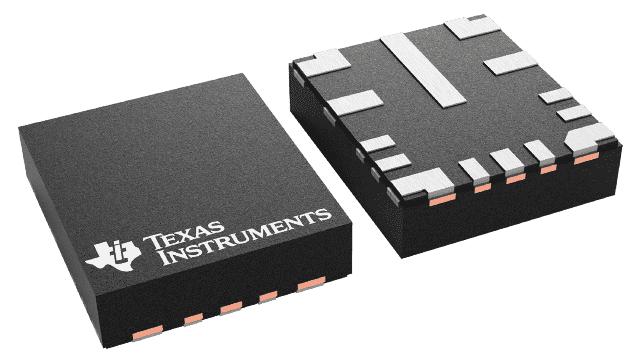
\includegraphics[width=.5\textwidth]{img/LM61460.png}
    \caption{The LM61460 in the VQFN-HR package.}
    \label{fig:LM61460} 
\end{figure}

The values for the schematic were obtained using the TI Workbench.

\subsubsection{The 8V Rail}

The TPS62932 from Texas Instruments was chosen as it is incredible small and has a current rating of $2$A. It also has an in built MOSFET in its incredible tiny package of just 2.1 mm $\times$ 1.6 mm.

\begin{figure}[H]
    \centering
    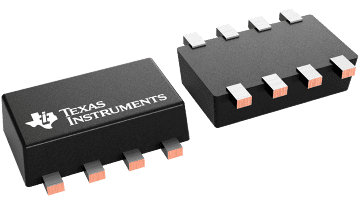
\includegraphics[width=.5\textwidth]{img/TPS62932.png}
    \caption{The TPS62932 in the SOT-583 package.}
    \label{fig:TPS62932} 
\end{figure}

The values for the schematic were obtained using the TI Workbench.

\subsection{The Schematic}

The first stage of the PCB development process is creating the schematic; the wiring diagram for all the connections. The first step is to add all the individual components that are used, the Raspberry Pi, the buck converter ICs, the motors, the LEDs, the switches, the power connectors and any other I/O that maybe needed. \\

The switching regulators need additional hardware, such as resistors and capacitors along with an inductor. The value of these components decide what voltage you get at the output. To find these values, the TI workbench tool was used. The TI workbench allows one to configure the parameters and then produces a schematic (Figure \ref{fig:TI_WB}). This is then used to set the value and the connections of the SMD components. \\

\begin{figure}[H]
    \centering
    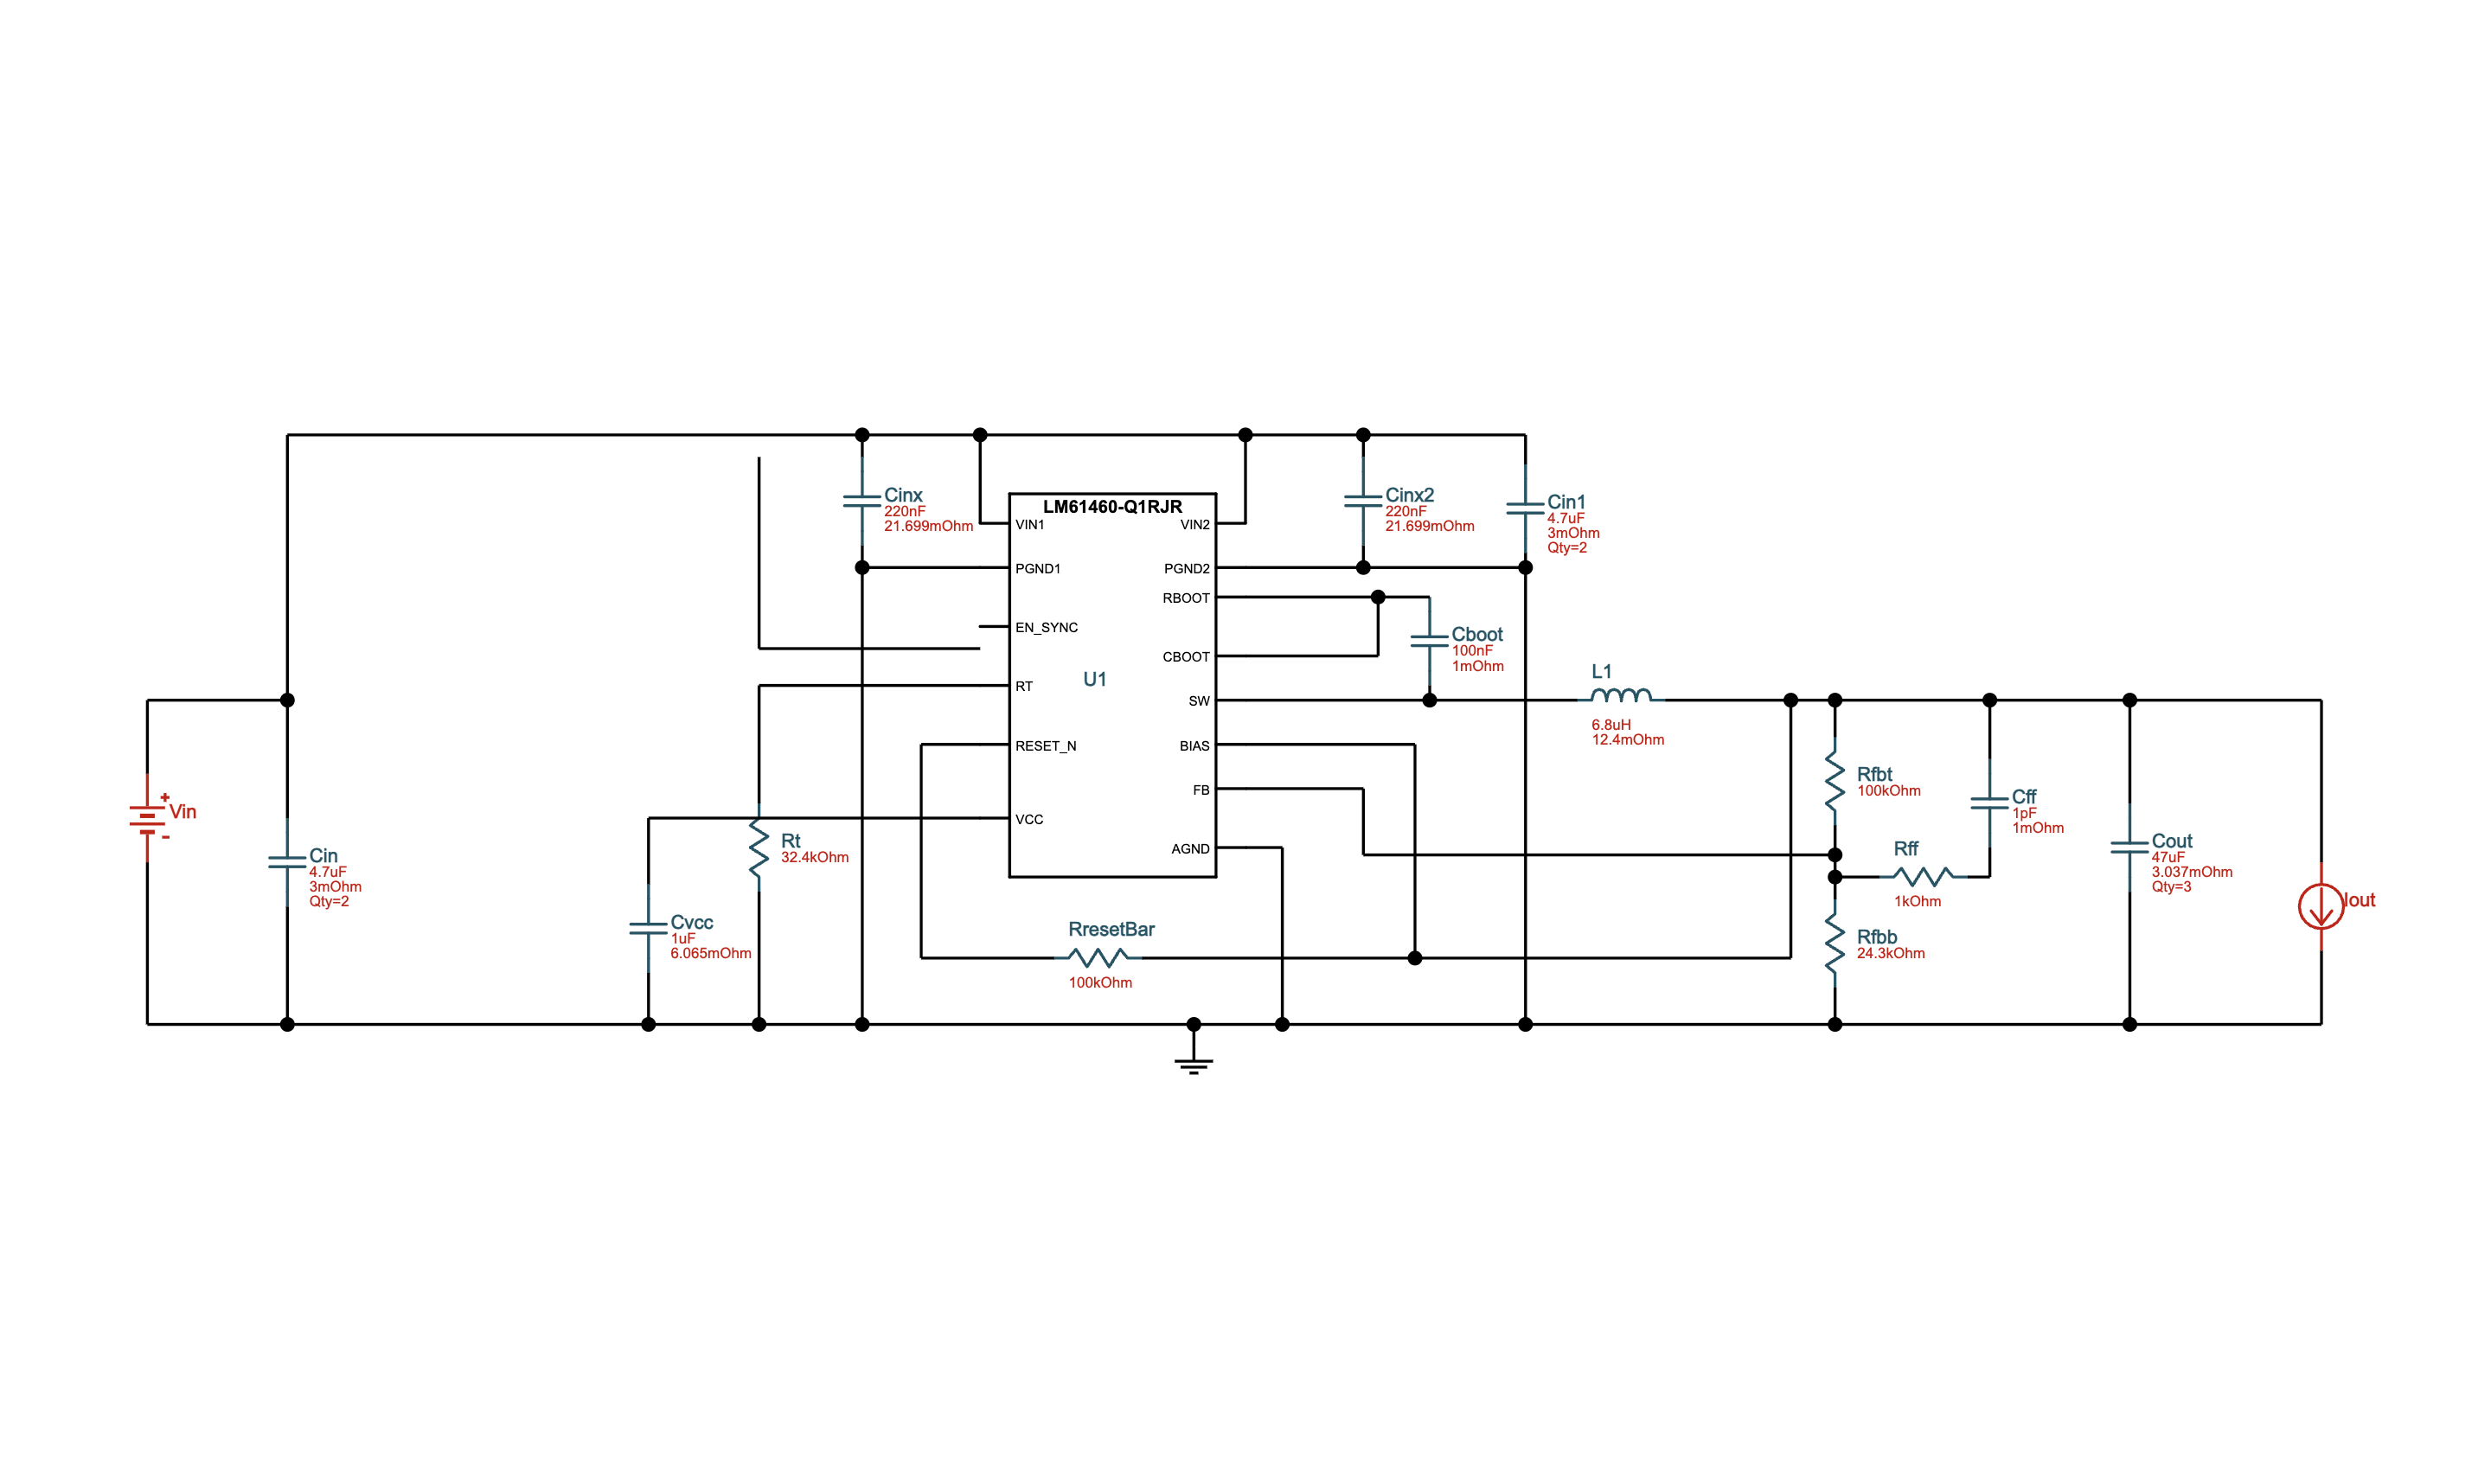
\includegraphics[width=1\textwidth]{img/TI_LM.png}
    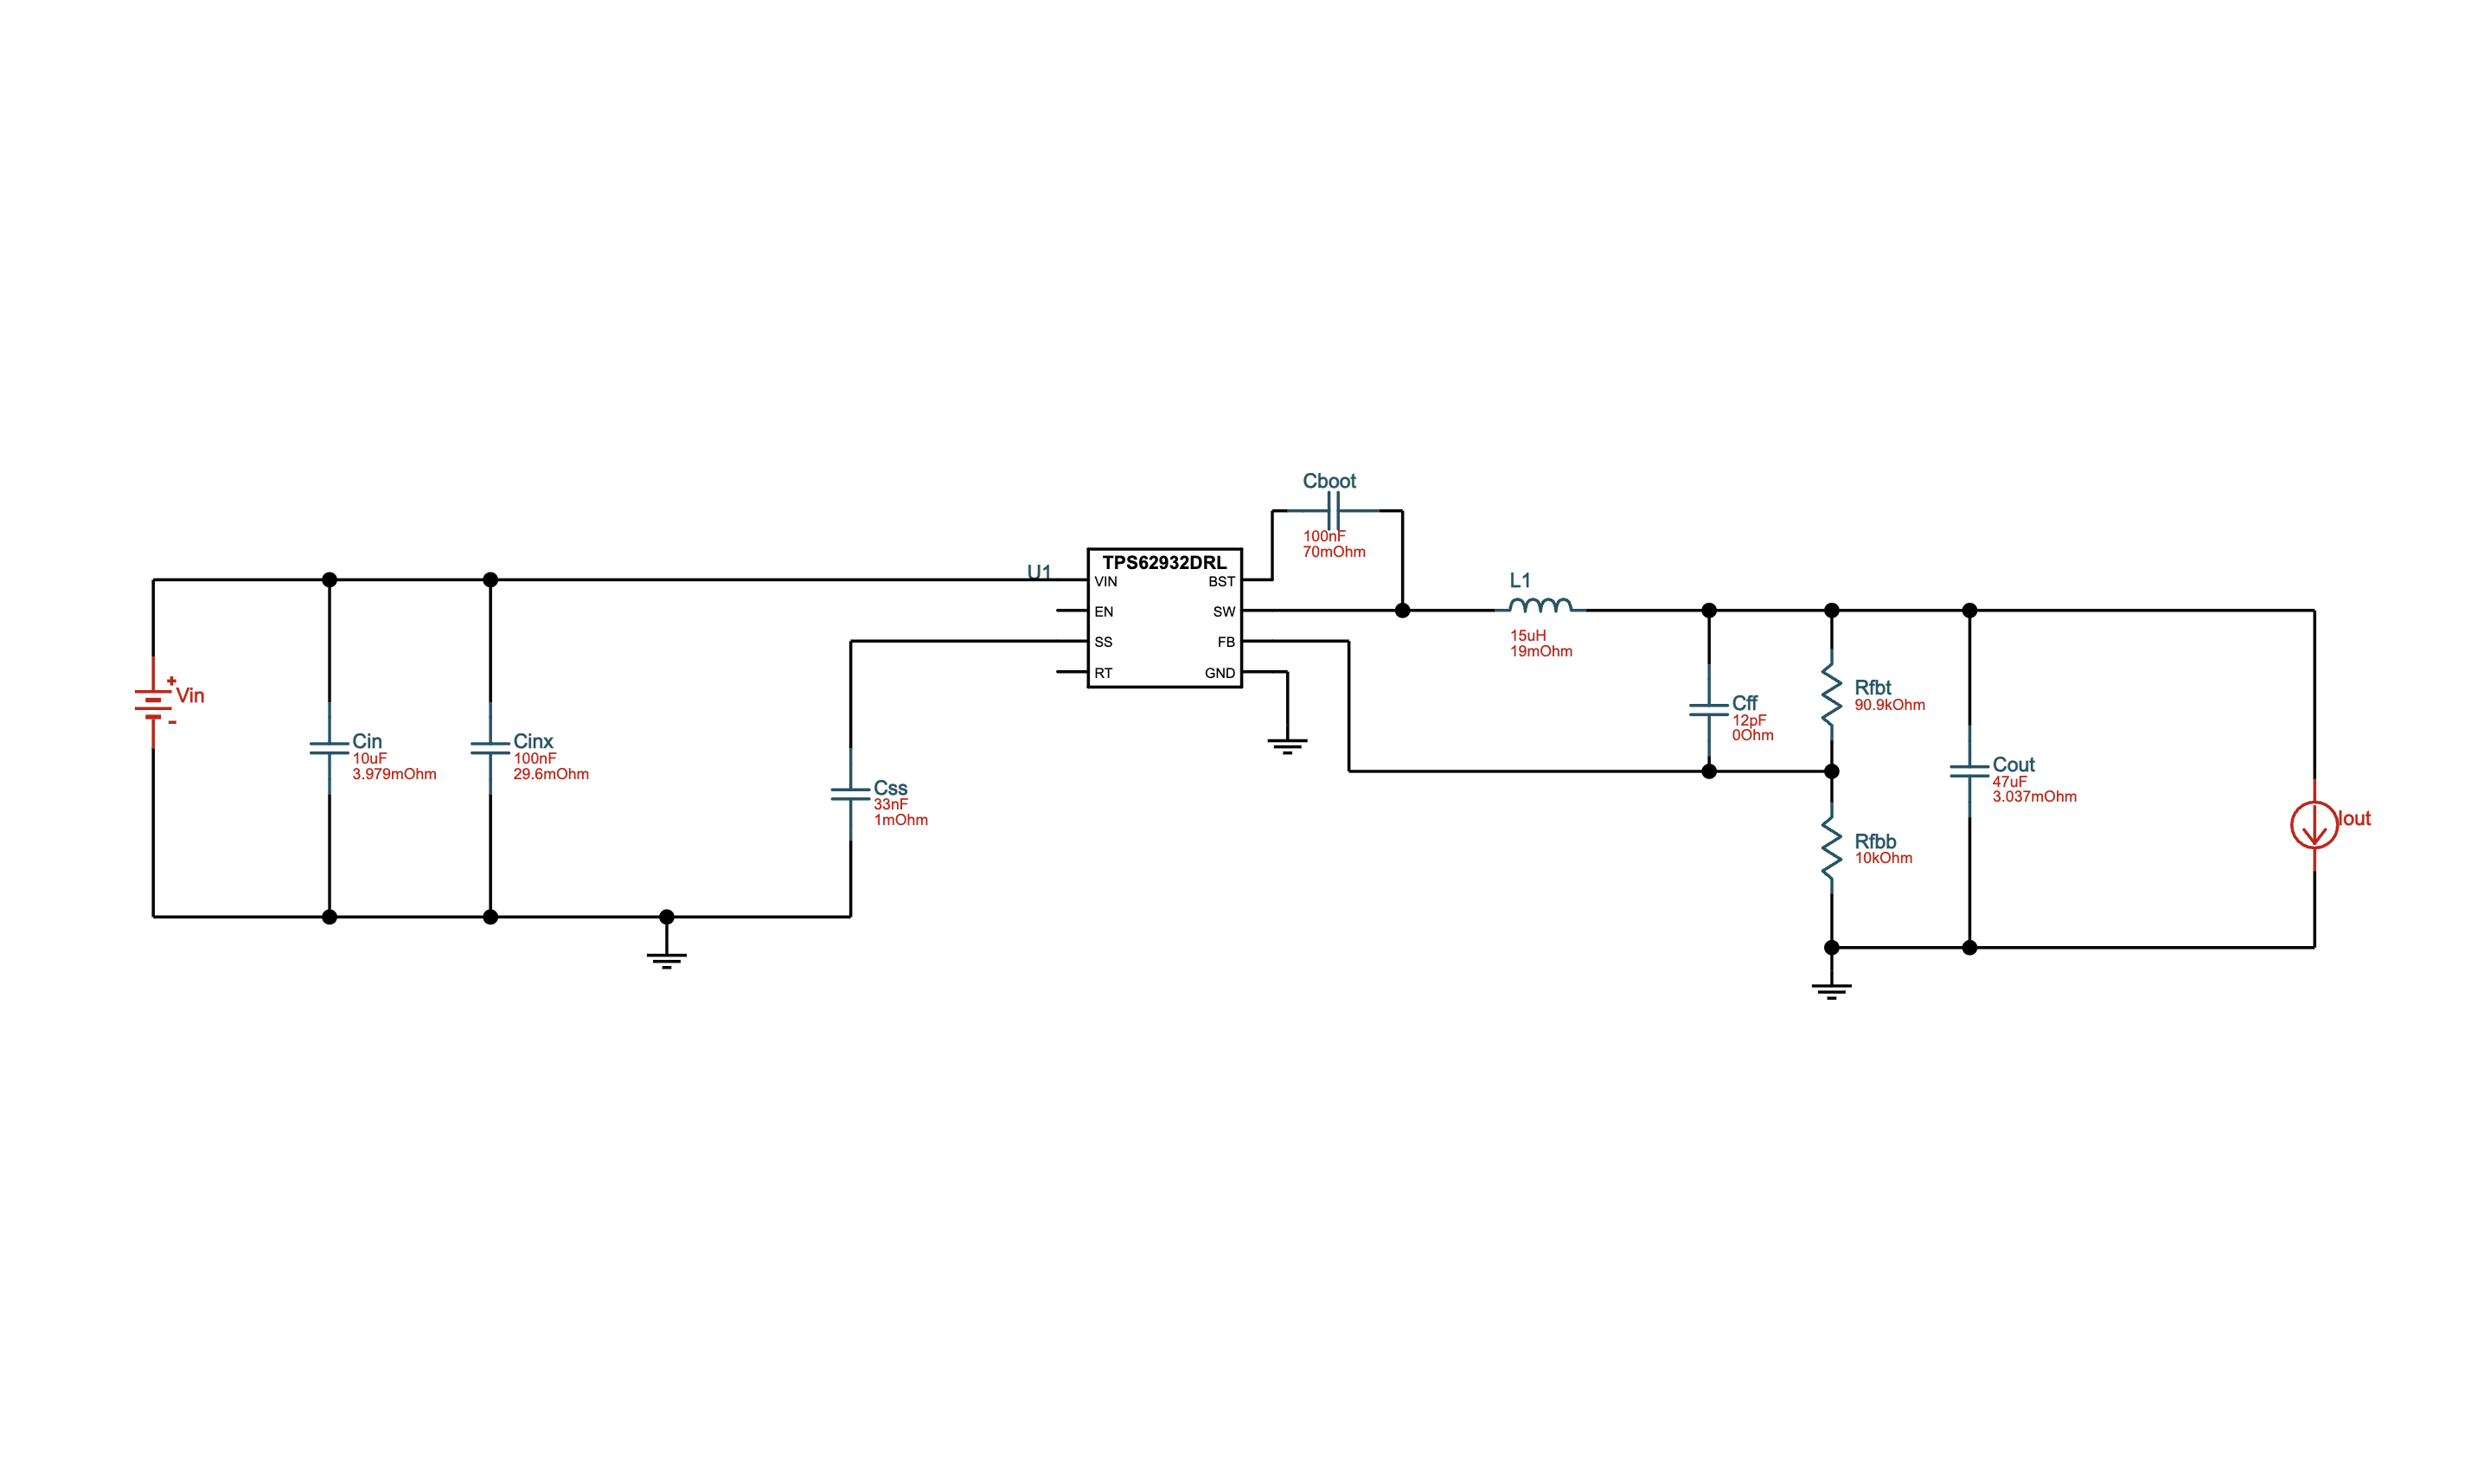
\includegraphics[width=1\textwidth]{img/TI_TPS.png}
    \caption{The files for the schematic given by TI Workbench.}
    \label{fig:TI_WB} 
\end{figure}

The schematic (Figure \ref{fig:Schematic}) created is in 3 pages. The main page has the XT30 power connector input and the power switch. The Raspberry Pi page consists of the Raspberry Pi, the sensors and I/O devices. The power page consists of all the power regulation circuitry. It also has 2 additional electrolytic capacitors, one $220 \mu \text{F}$ and the other $270 \mu \text{F}$. They both act as decoupling capacitors for the Raspberry Pi and the servo respectively. They ensure that when there are load spikes from either devices, the Raspberry Pi booting or the servo starting to move, the spike does not reach the ICs and is handled locally.

\begin{figure}[H]
    \centering
    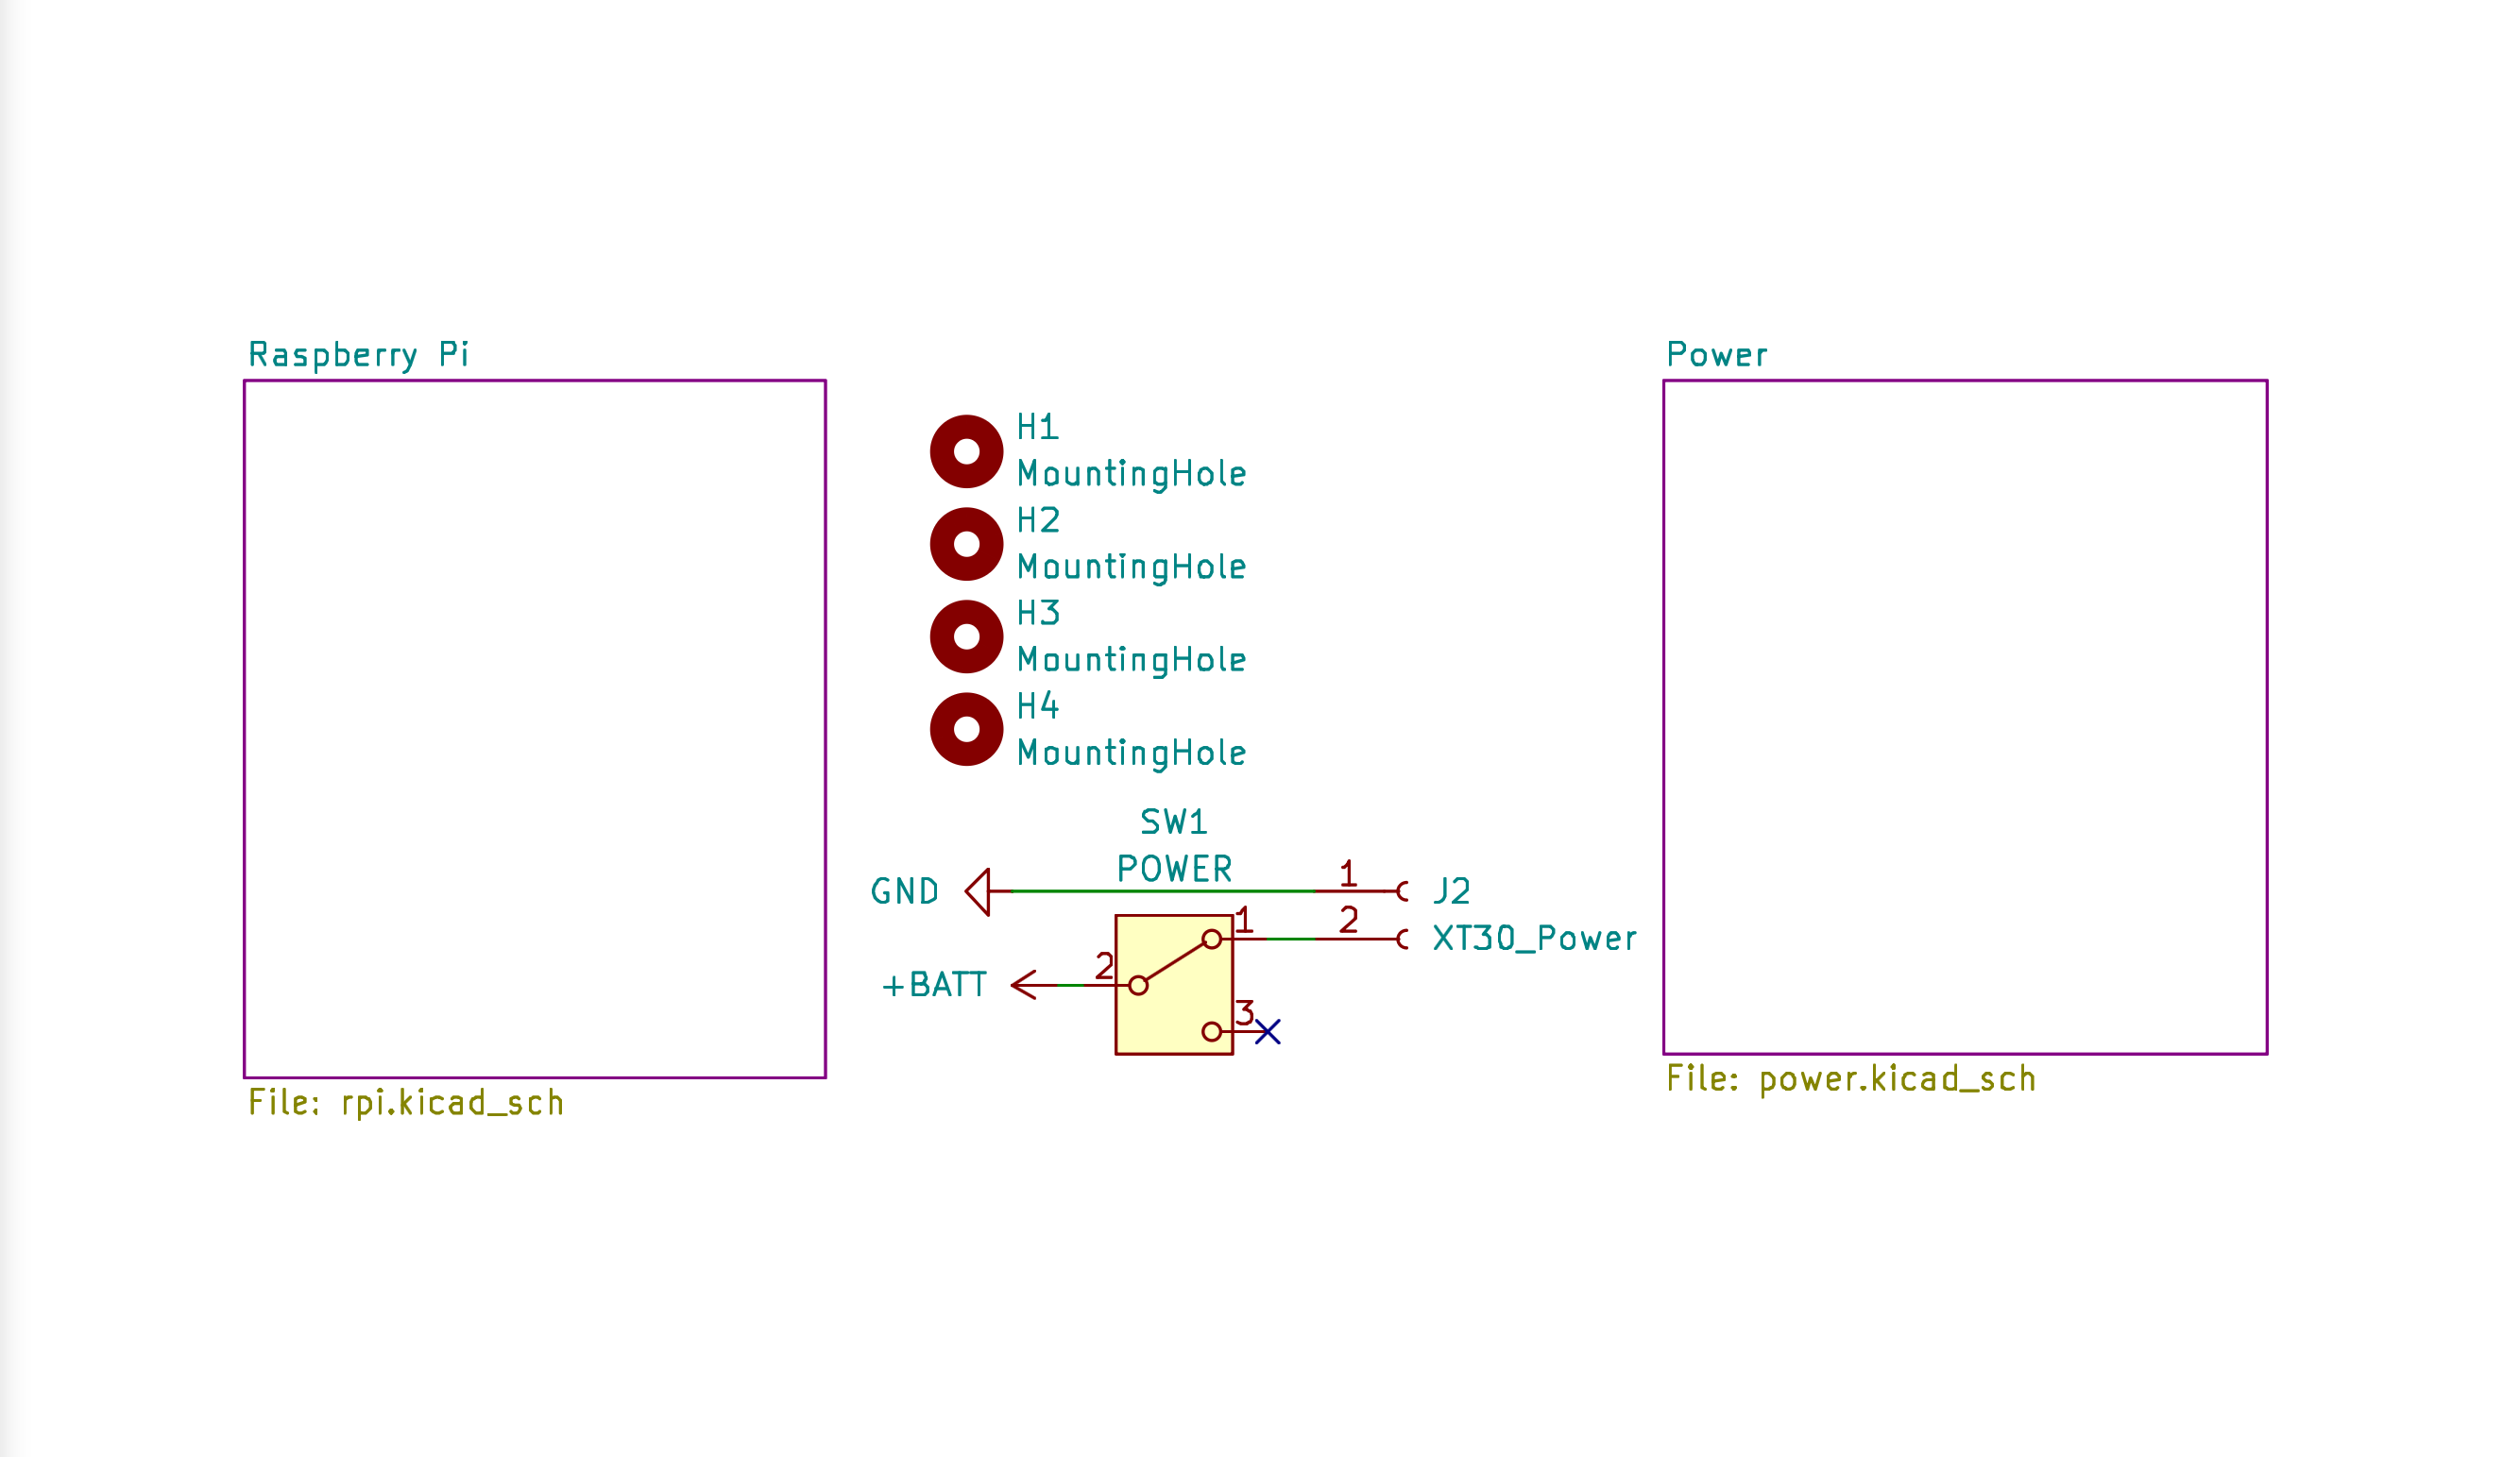
\includegraphics[width=.65\textwidth]{img/sch1.png}
    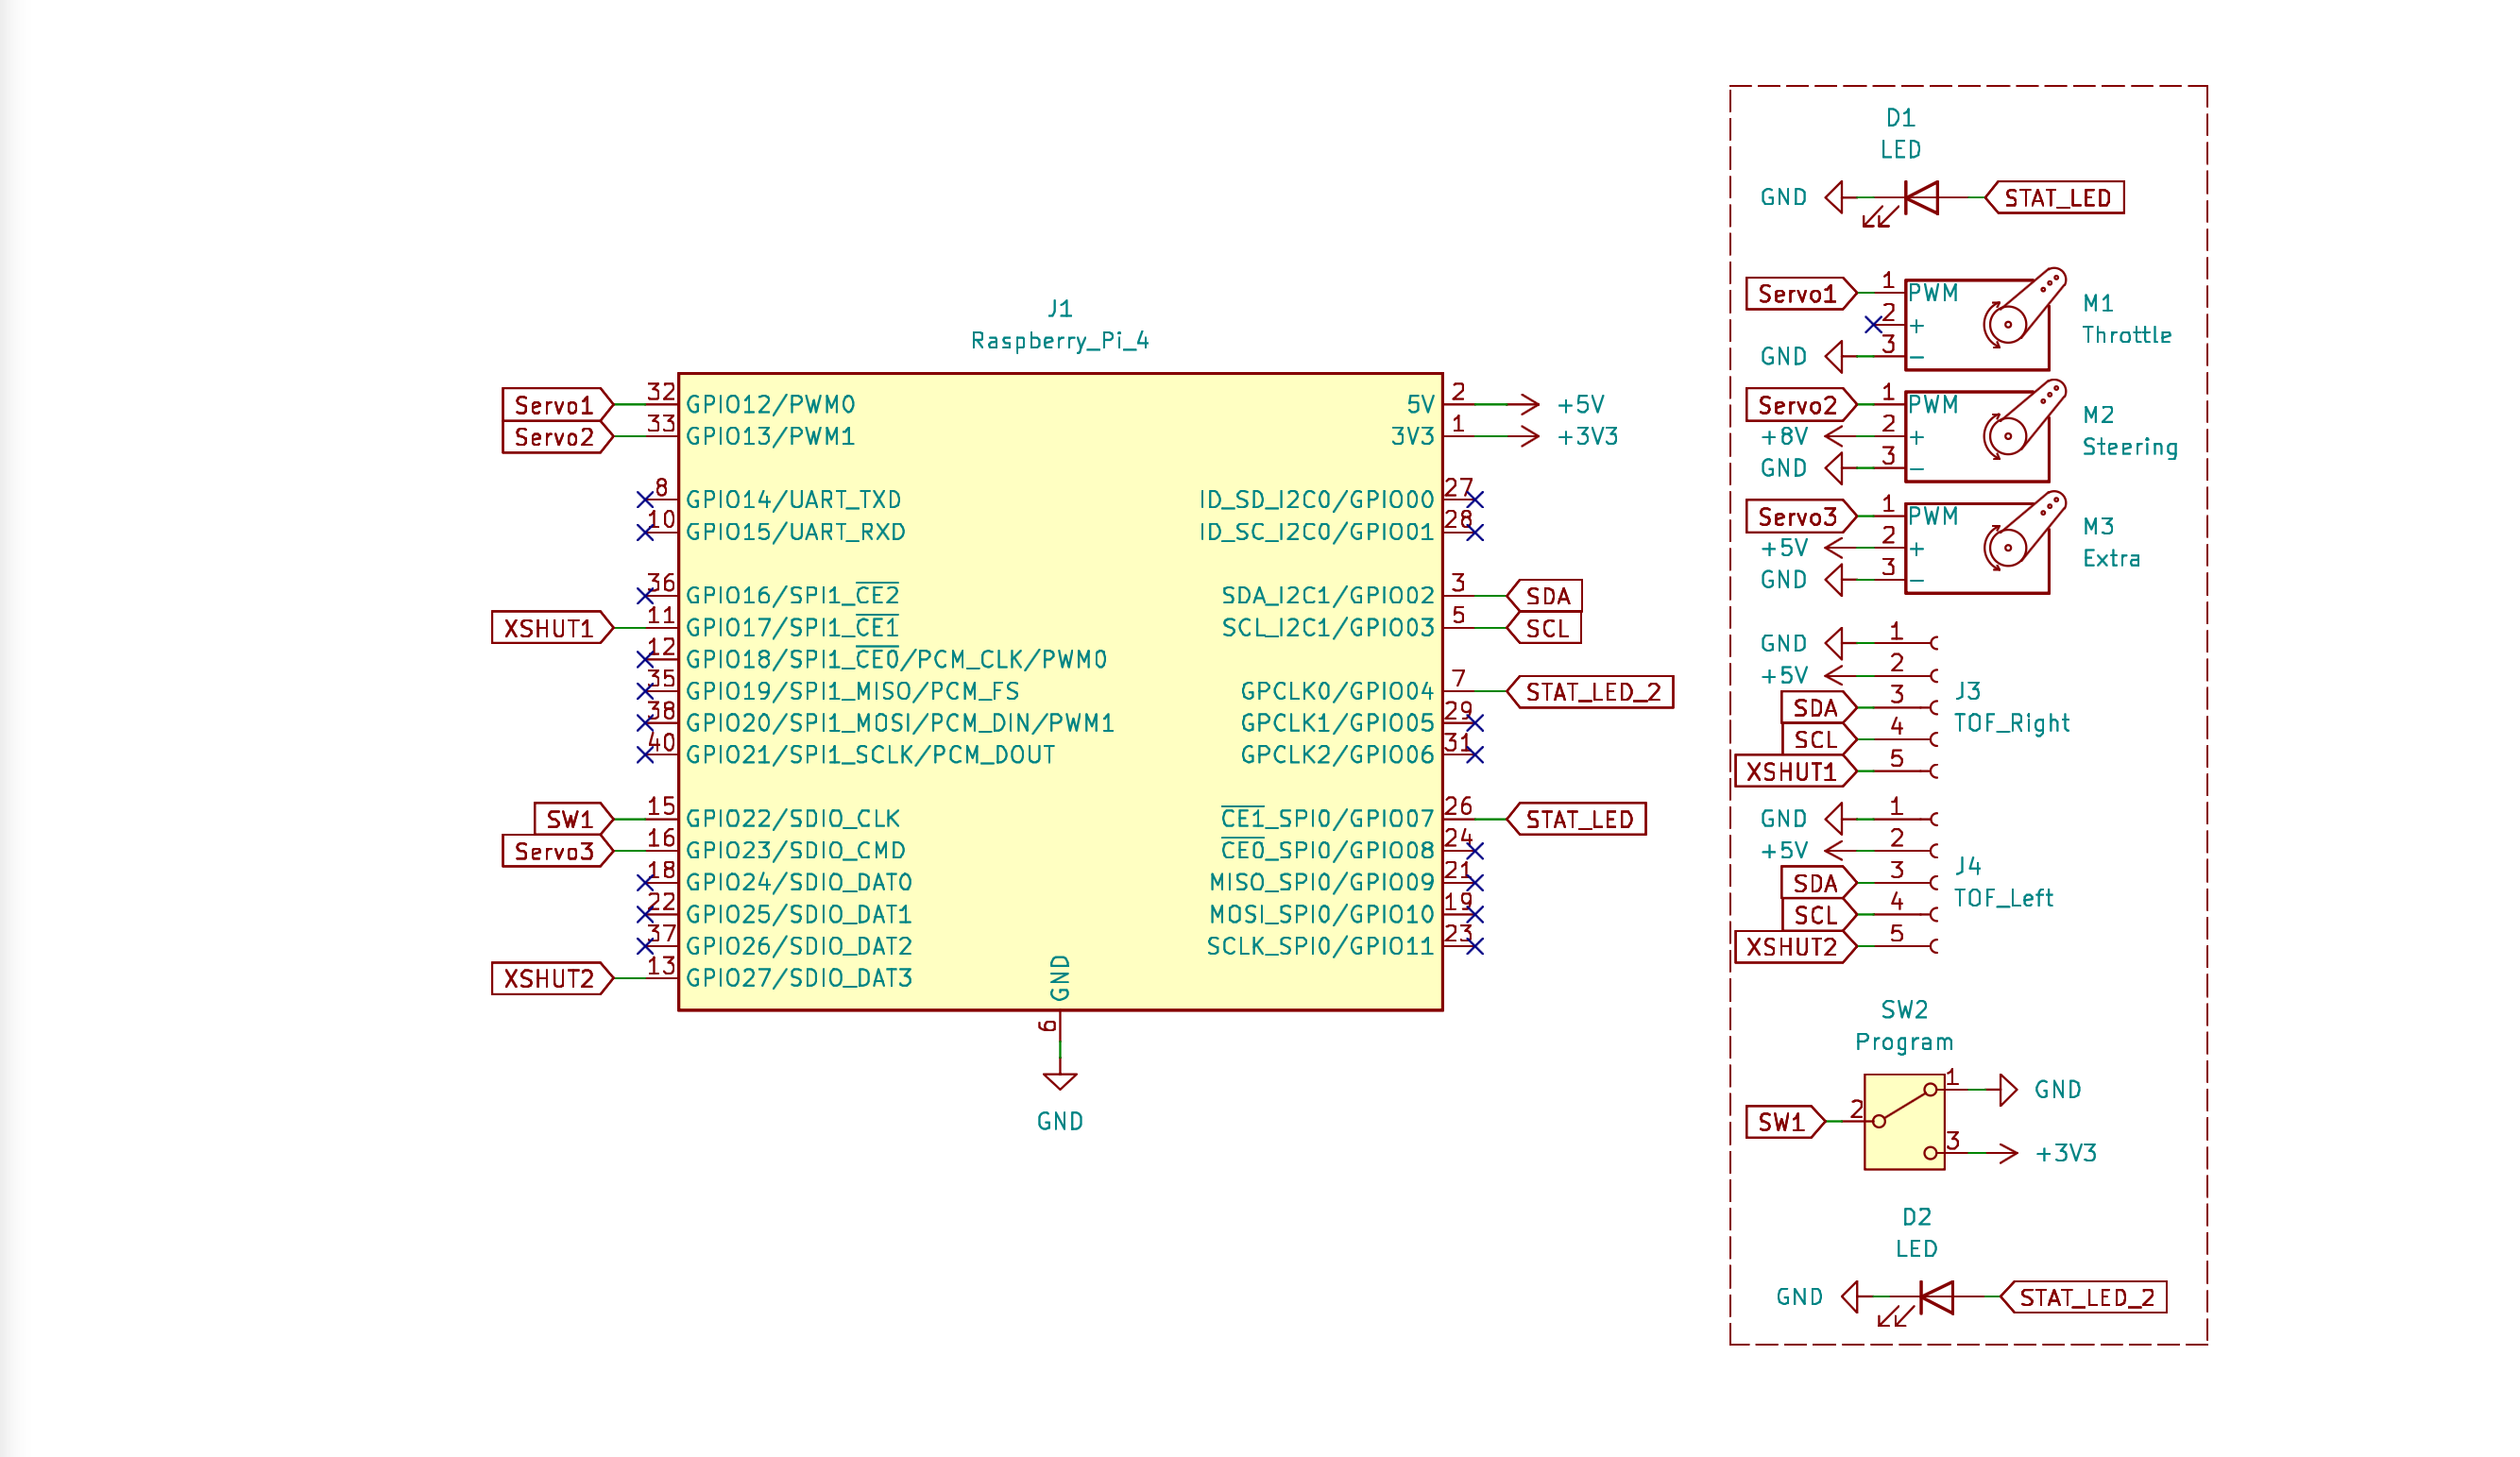
\includegraphics[width=.65\textwidth]{img/sch2.png}
    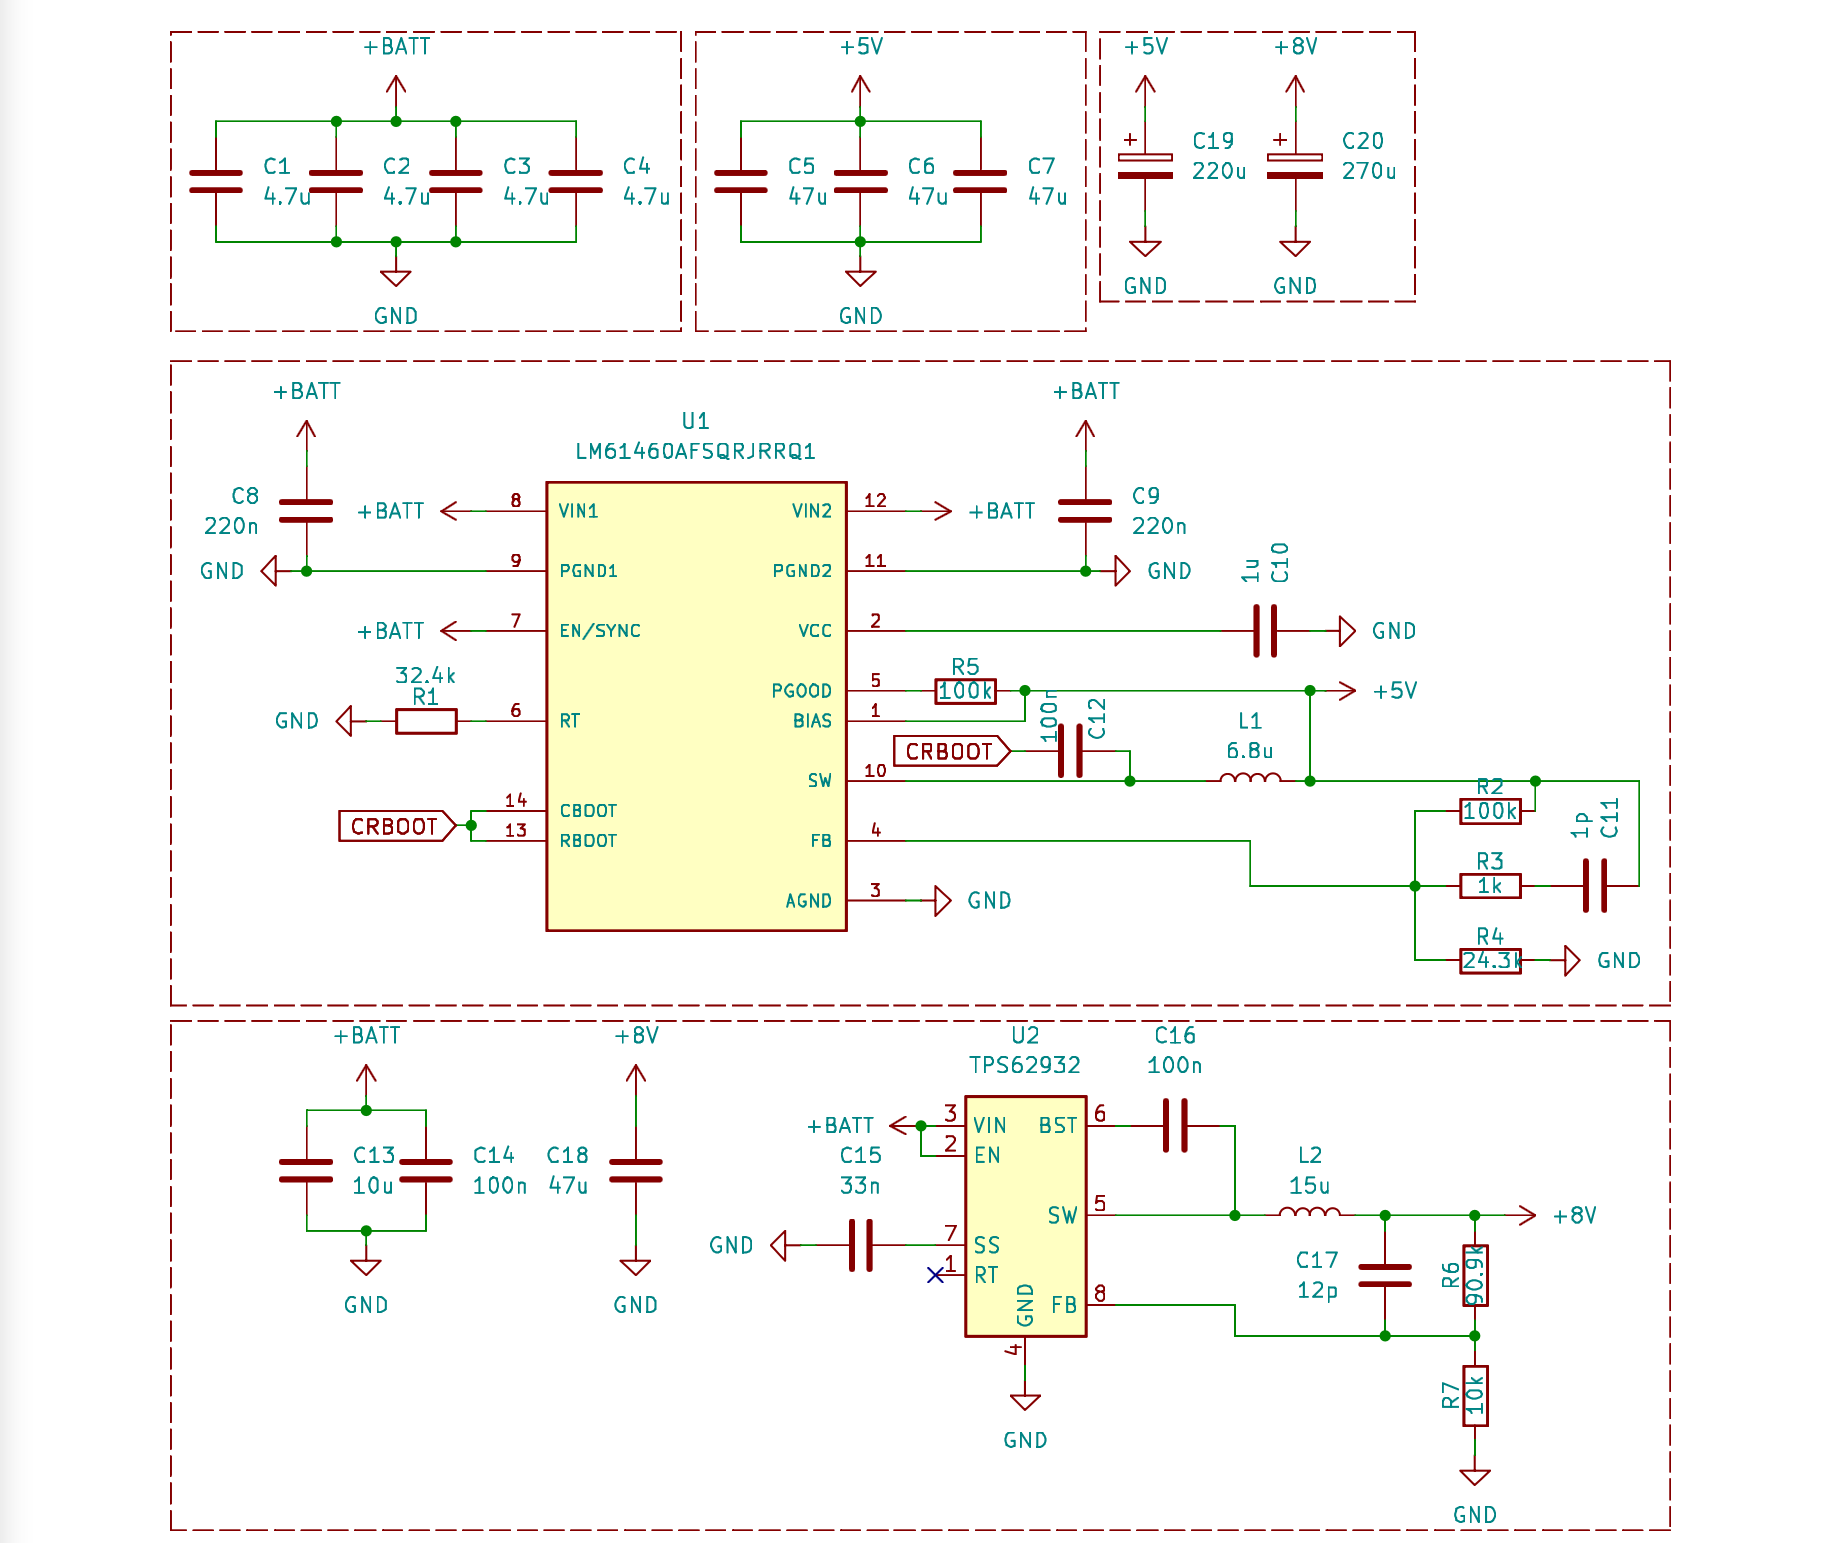
\includegraphics[width=.65\textwidth]{img/sch3.png}
    \caption{The 3 pages of the schematic.}
    \label{fig:Schematic} 
\end{figure}

The PDF for the Schematic can also be found in the PCBA folder. The BOM for all the parts is also available there, along with the manufacturer used.

\subsection{The Layout \& Routing}

This step is very crucial, it is responsible for how well the components interact with each-other and determines how clean your output voltage is. A \textbf{4 layer board} was chosen. This was done as it would make the routing easier across multiple layers and because a 4 layer stack up is recommended in the LM61460 data sheet. \\

All the SMD components would be place on one side of the board so that the board could be assembled on a hot plate. This would also aid with the ease of assembly. The following is the stack up $\rightarrow$

\begin{enumerate}
\item Layer 1: It carries much of the important \textbf{signals}, especially for the buck converters.
\item Layer 2: A solid \textbf{Ground} plane to reduce EMI and act as a fast return path of the top player.
\item Layer 3: The \textbf{Power} plane consisting of the input voltage, $5.15$V and $8$V.
\item Layer 4: A \textbf{Ground} plane that also carried some of the \textbf{signals} from the Raspberry Pi.
\end{enumerate}

The first thing to do is create the board outline. A rounded rectangle with length $65$mm, height $56$mm and a corner radius of $2$mm was chosen. A $6$mm notch was then removed from the bottom right of the board to allow the camera ribbon cable to pass through. Figure \ref{fig:Outline} shows the shape of the board.

\begin{figure}[H]
    \centering
    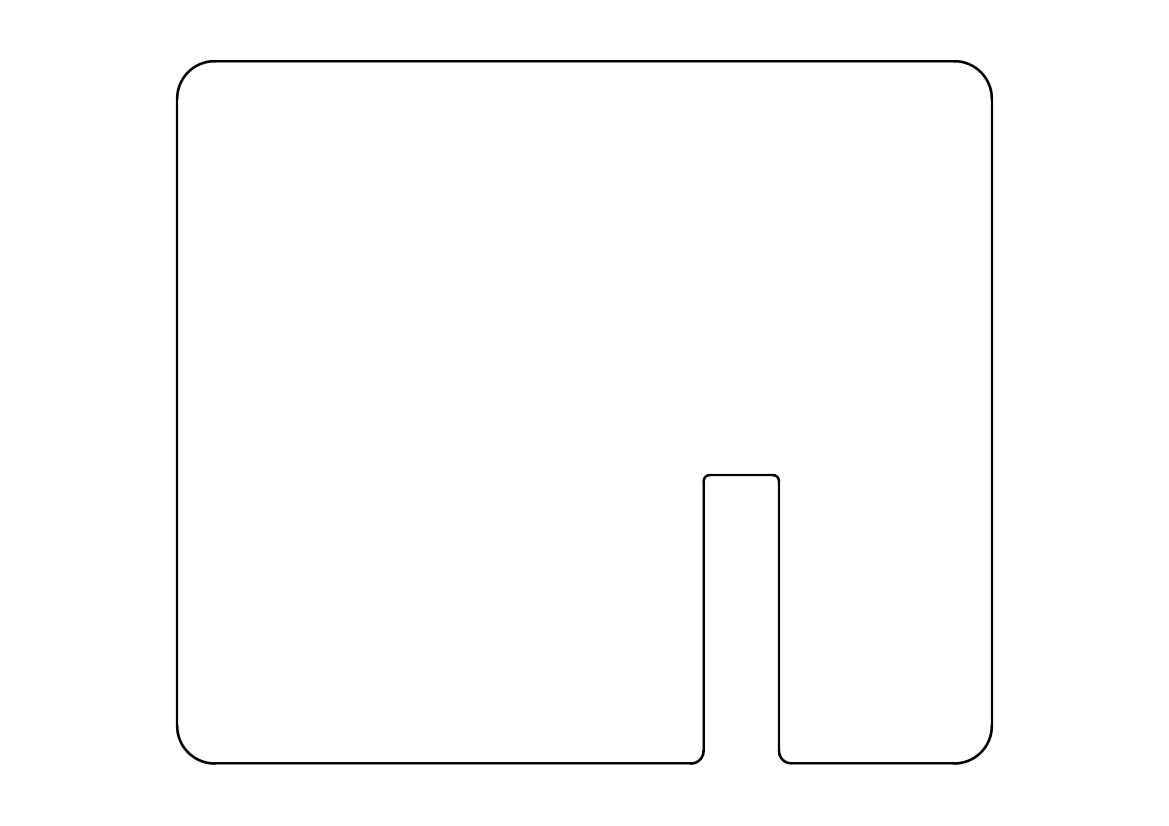
\includegraphics[width=.65\textwidth]{img/outline.png}
    \caption{The "edge cuts" layer.}
    \label{fig:Outline} 
\end{figure}

After this, the fixed components are place, such as the mounting holes for the board and the $20 \times 2$ female header pin that connects to the Raspberry Pi. These need to be incredibly precise as they are the locating hardware for the hat to connect on to the Raspberry Pi. M$2.5$ holes are used.

\begin{figure}[H]
    \centering
    \includegraphics[width=.65\textwidth]{img/fixed_items.png}
    \caption{The fixed items layer.}
    \label{fig:Fixed_Items_PCB} 
\end{figure}

The next part is the most cumbersome. All the physical parts need to be laid out in a manner that ensures the most ideal connections possible. The 3 main current loops; ON-State Current Loop, OFF-State Current Loop and The "Hot Loop"; of the buck converter need to be kept as short as possible. Since we are using a symmetric buck converter, it also needs to be made sure that the power lines to both sides are as similar as they can be. The path between the switching node and the inductor needs to be as short as possible. All the connectors need to accessible. \\

For this reason, the power connector (XT30) and the power switch were placed on the right side. The switching circuitry was spread around the middle. The second switch and the connectors for the motor and servo were kept on the left side. The electrolytic capacitors were placed as close to the outputs as possible. The LEDs were also placed in the middle. The extra components, such as the connectors for the 2 ToF sensors and an extra PWM connector were kept on the bottom and bottom right respectively. Figure \ref{fig:Layout} shows the layout of the final board. It is fairly crammed but a lot more items, such as more LEDs, Current and Voltage sensing and a CAN BUS port can also be added in the future.

\begin{figure}[H]
    \centering
    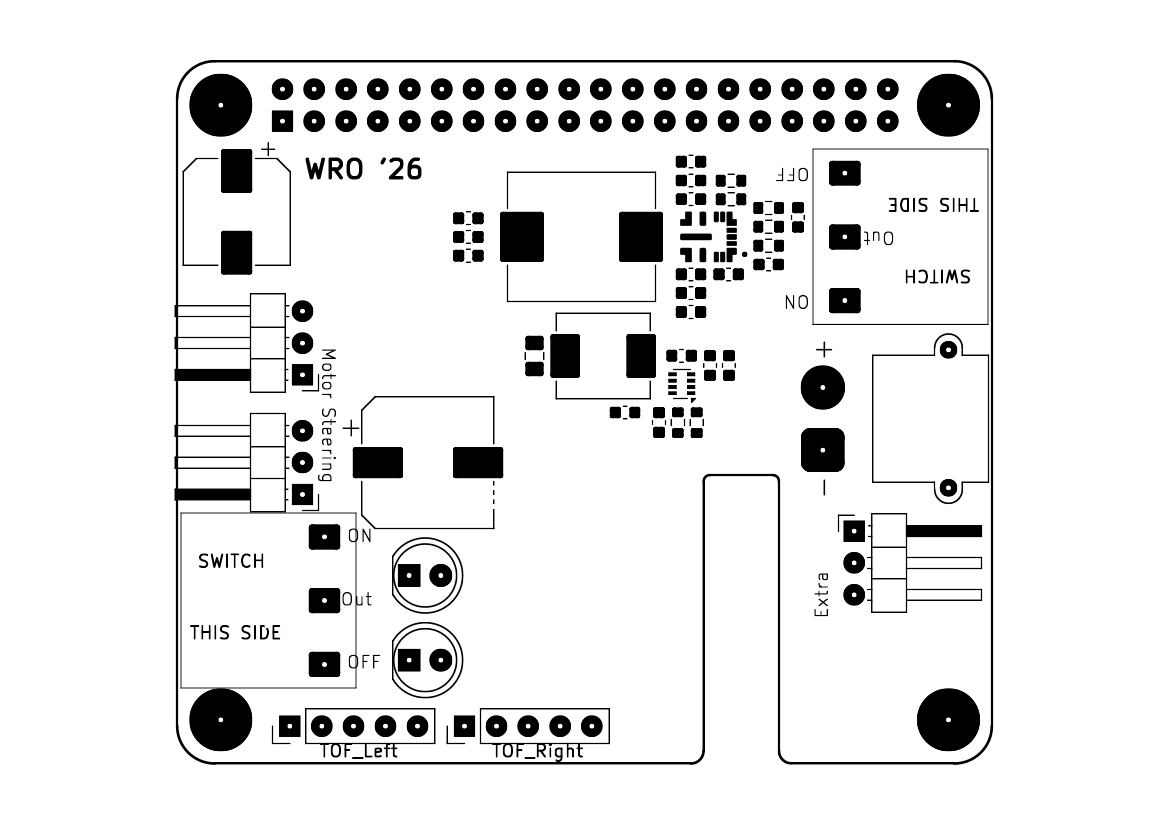
\includegraphics[width=.8\textwidth]{img/Layout.png}
    \caption{The final layout depicting the placement of all the components.}
    \label{fig:Layout} 
\end{figure}

Figure \ref{fig:Layers} shows the actual copper layers as they are. Copper pours are preferred whenever possible. They also help with thermal management. It was made sure that there were no wires beneath the two inductors to make sure all the signal traces are as clean as possible.

\begin{figure}[H]
    \centering
    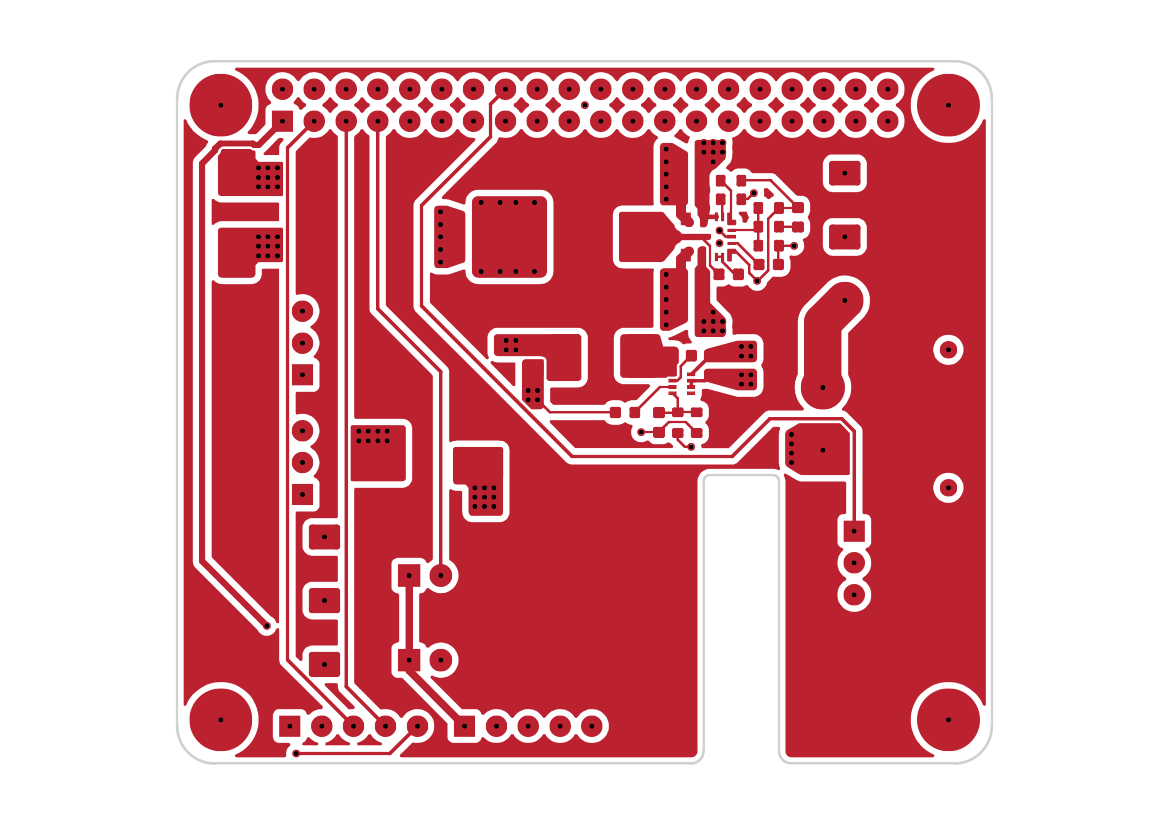
\includegraphics[width=.6\textwidth]{img/l1.png}
\end{figure}

\begin{figure}[H]
    \centering
    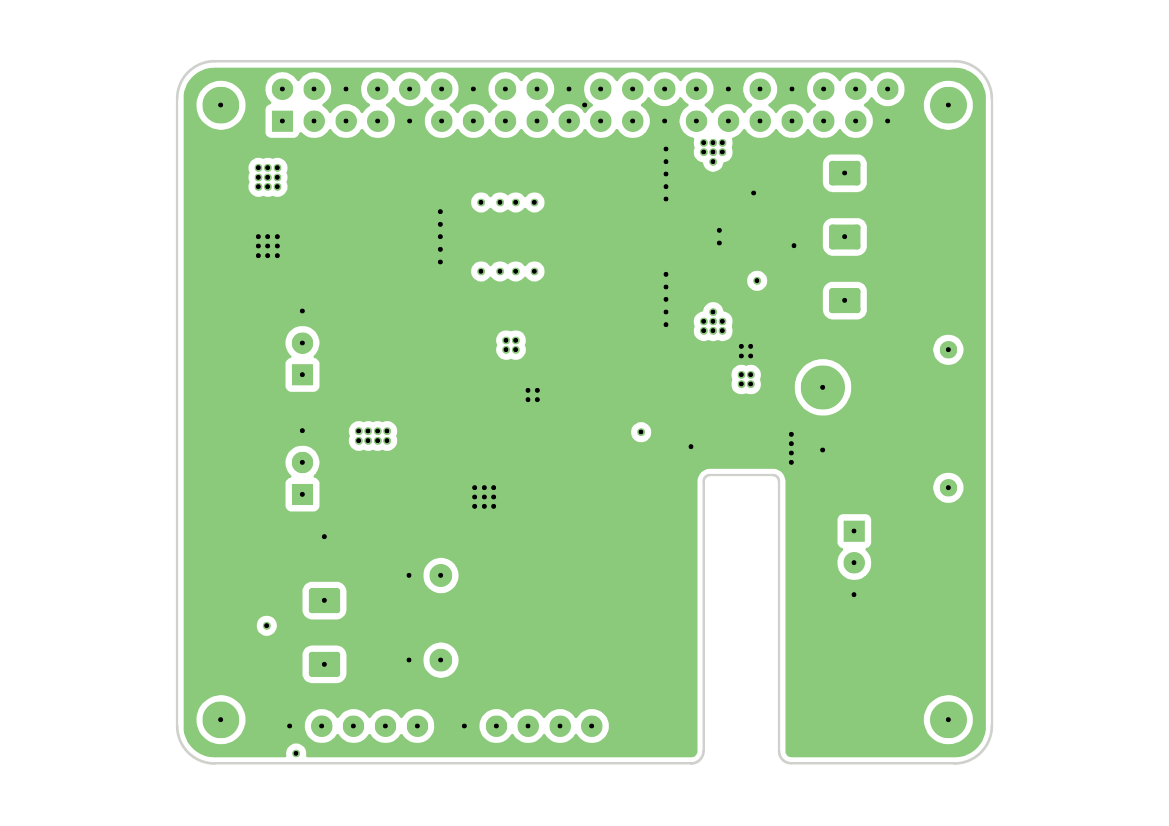
\includegraphics[width=.6\textwidth]{img/l2.png}
    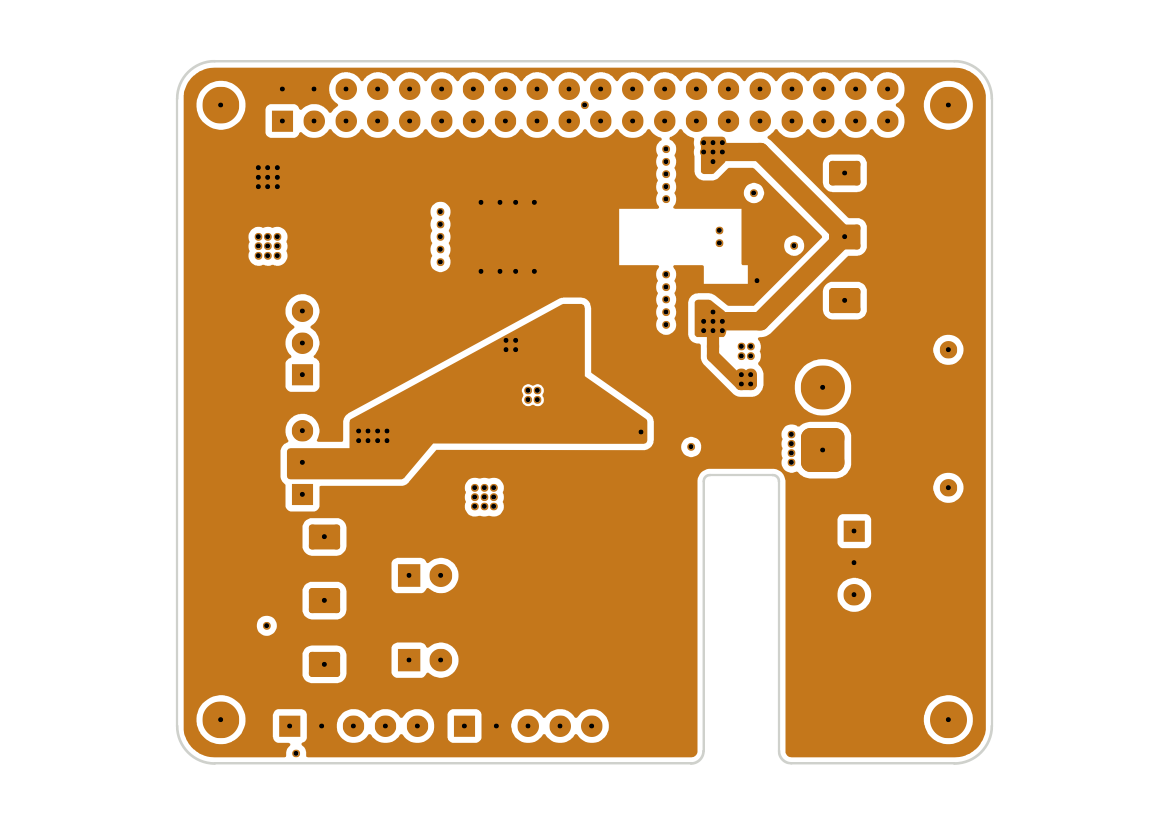
\includegraphics[width=.6\textwidth]{img/l3.png}
    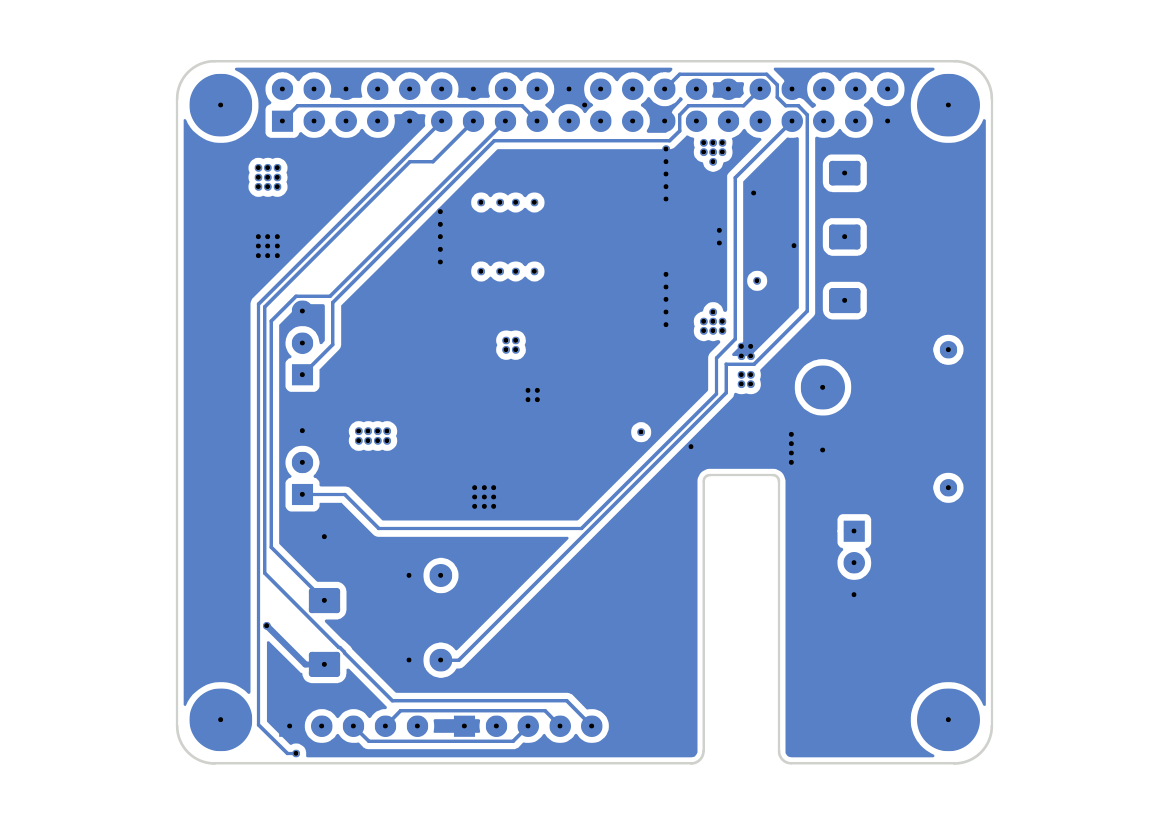
\includegraphics[width=.6\textwidth]{img/l4.png}
    \caption{The 4 copper layers. Layer$1$ $\rightarrow$ $4$.}
    \label{fig:Layers} 
\end{figure}

Some art work and quotes were added to the free space to ensure complete utilization and occupation of left over space. A black solder mask was chosen. Figure \ref{fig:KiCAD_Render} show the PCB rendered in the KiCAD 3D viewer. The contribution for the art work goes to M.C. Escher.

\begin{figure}[H]
    \centering
    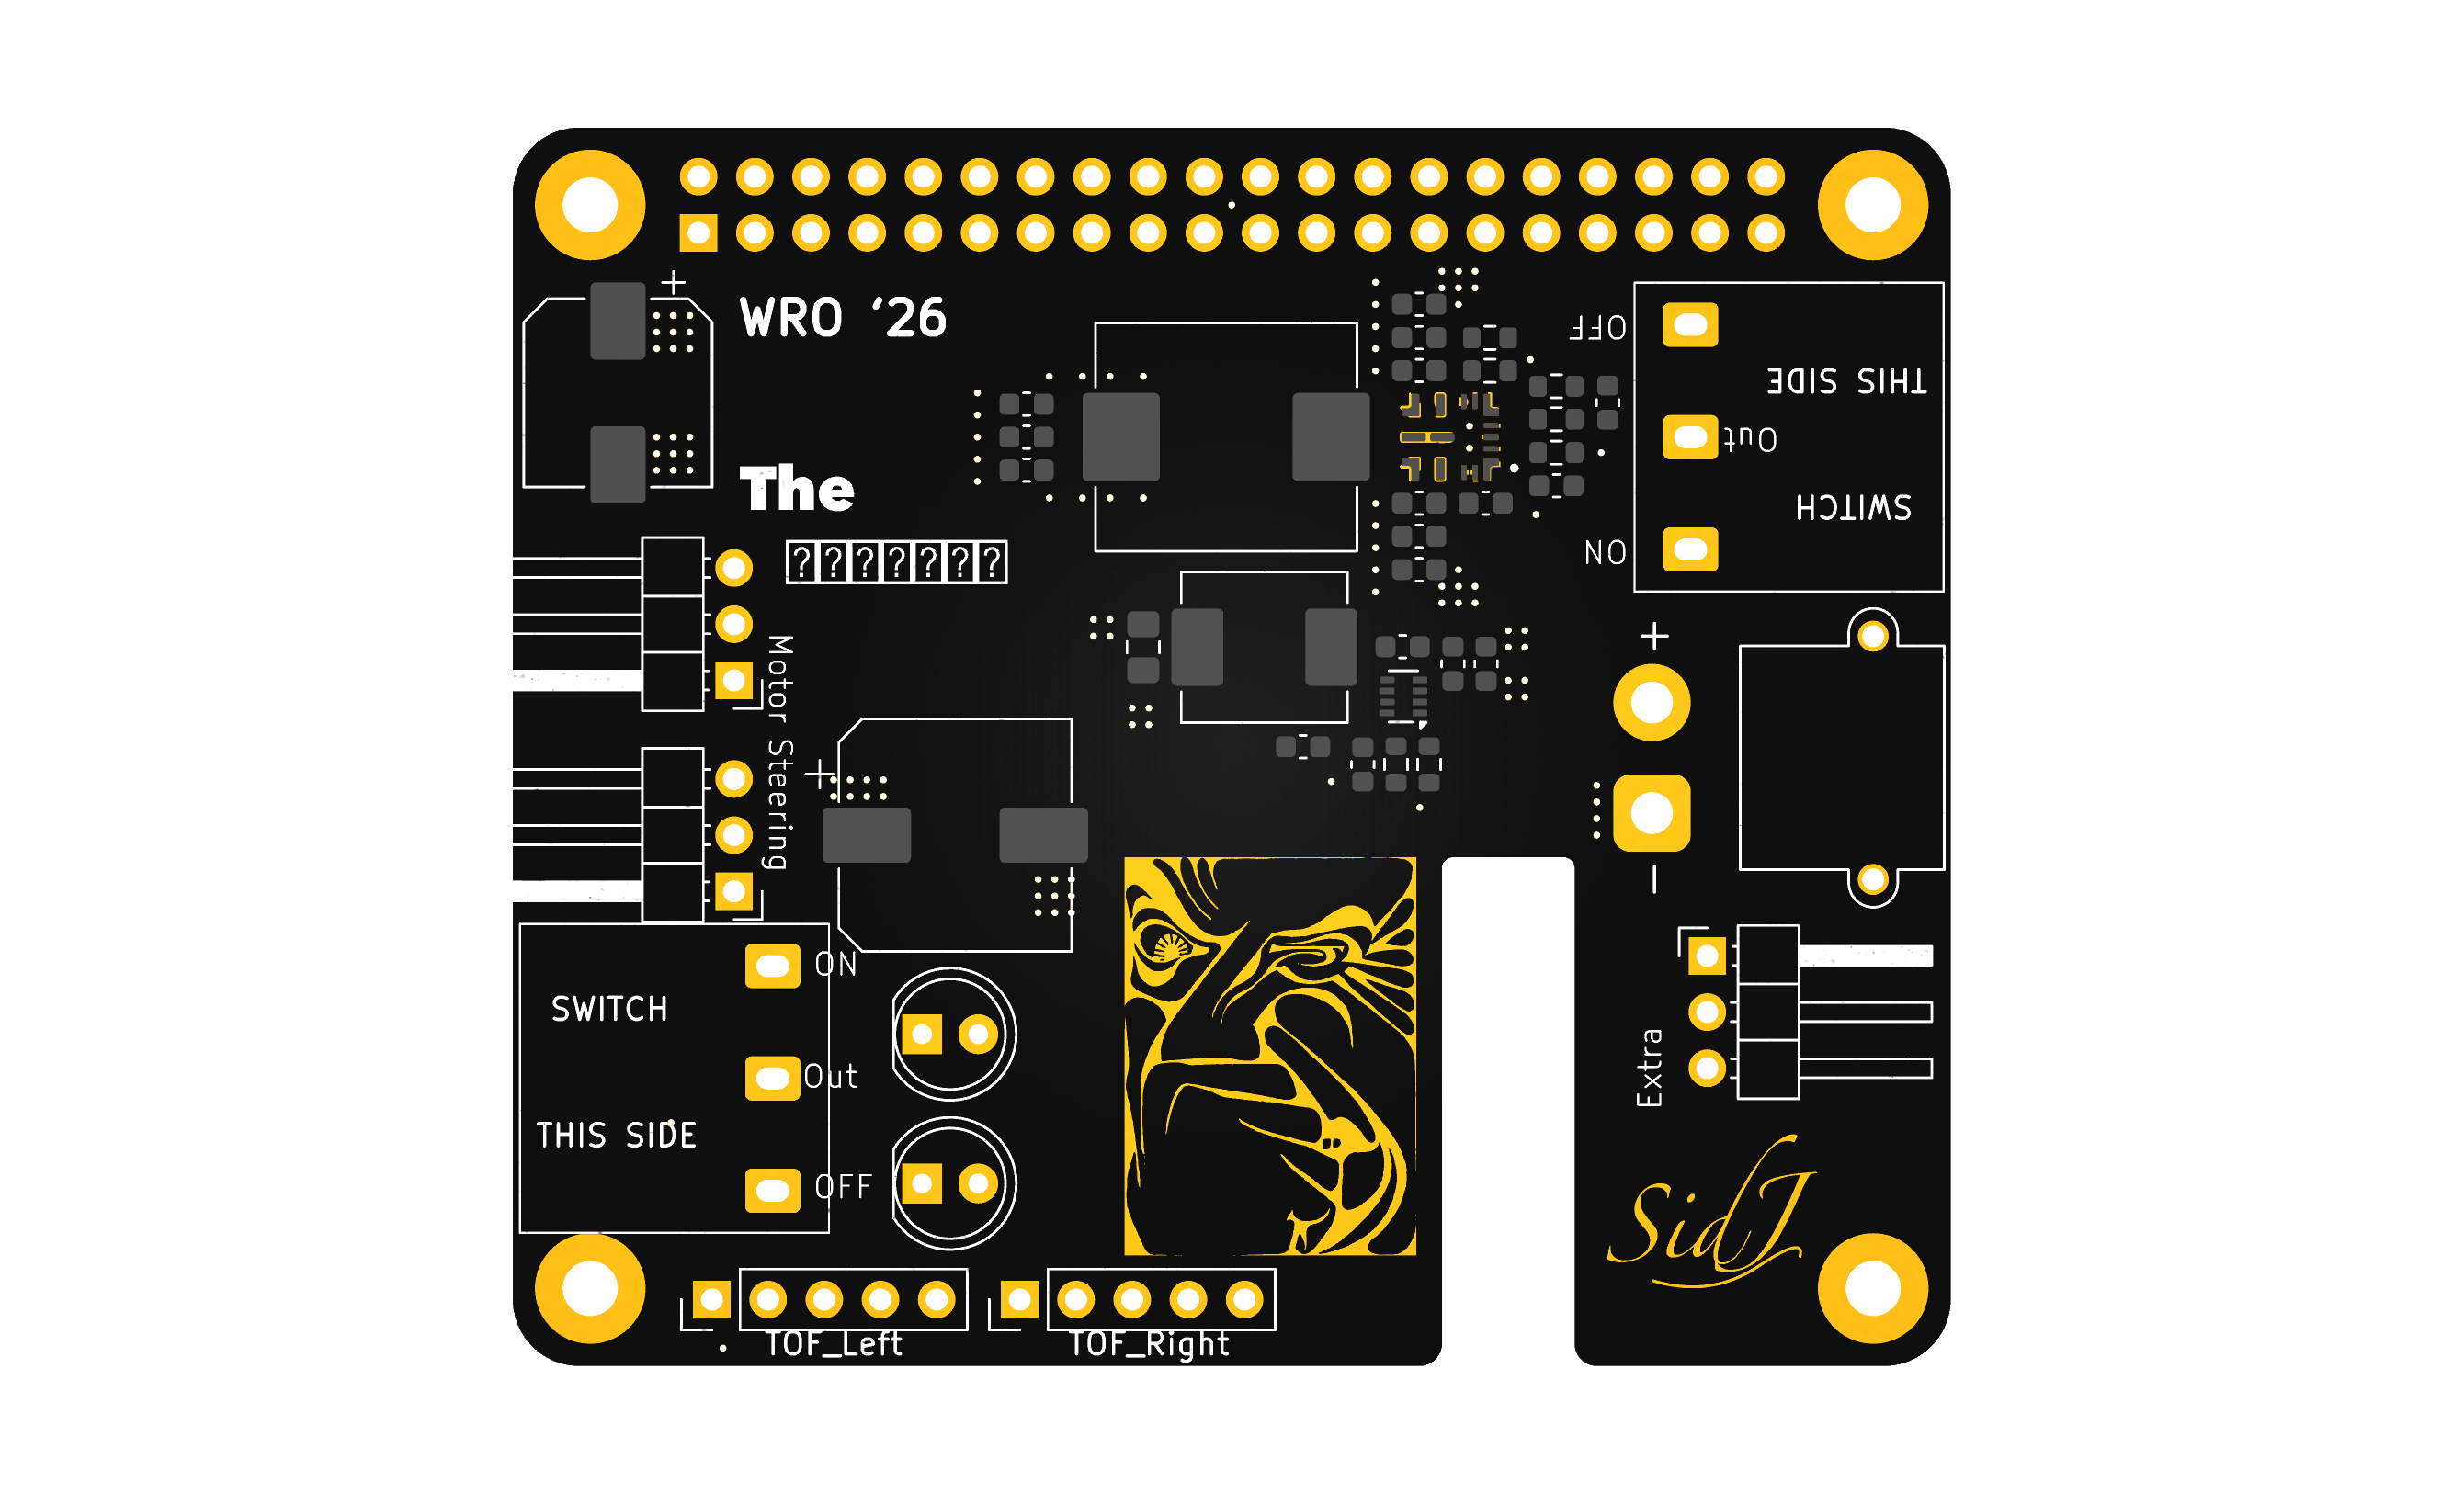
\includegraphics[width=1\textwidth]{img/top_render.png}
    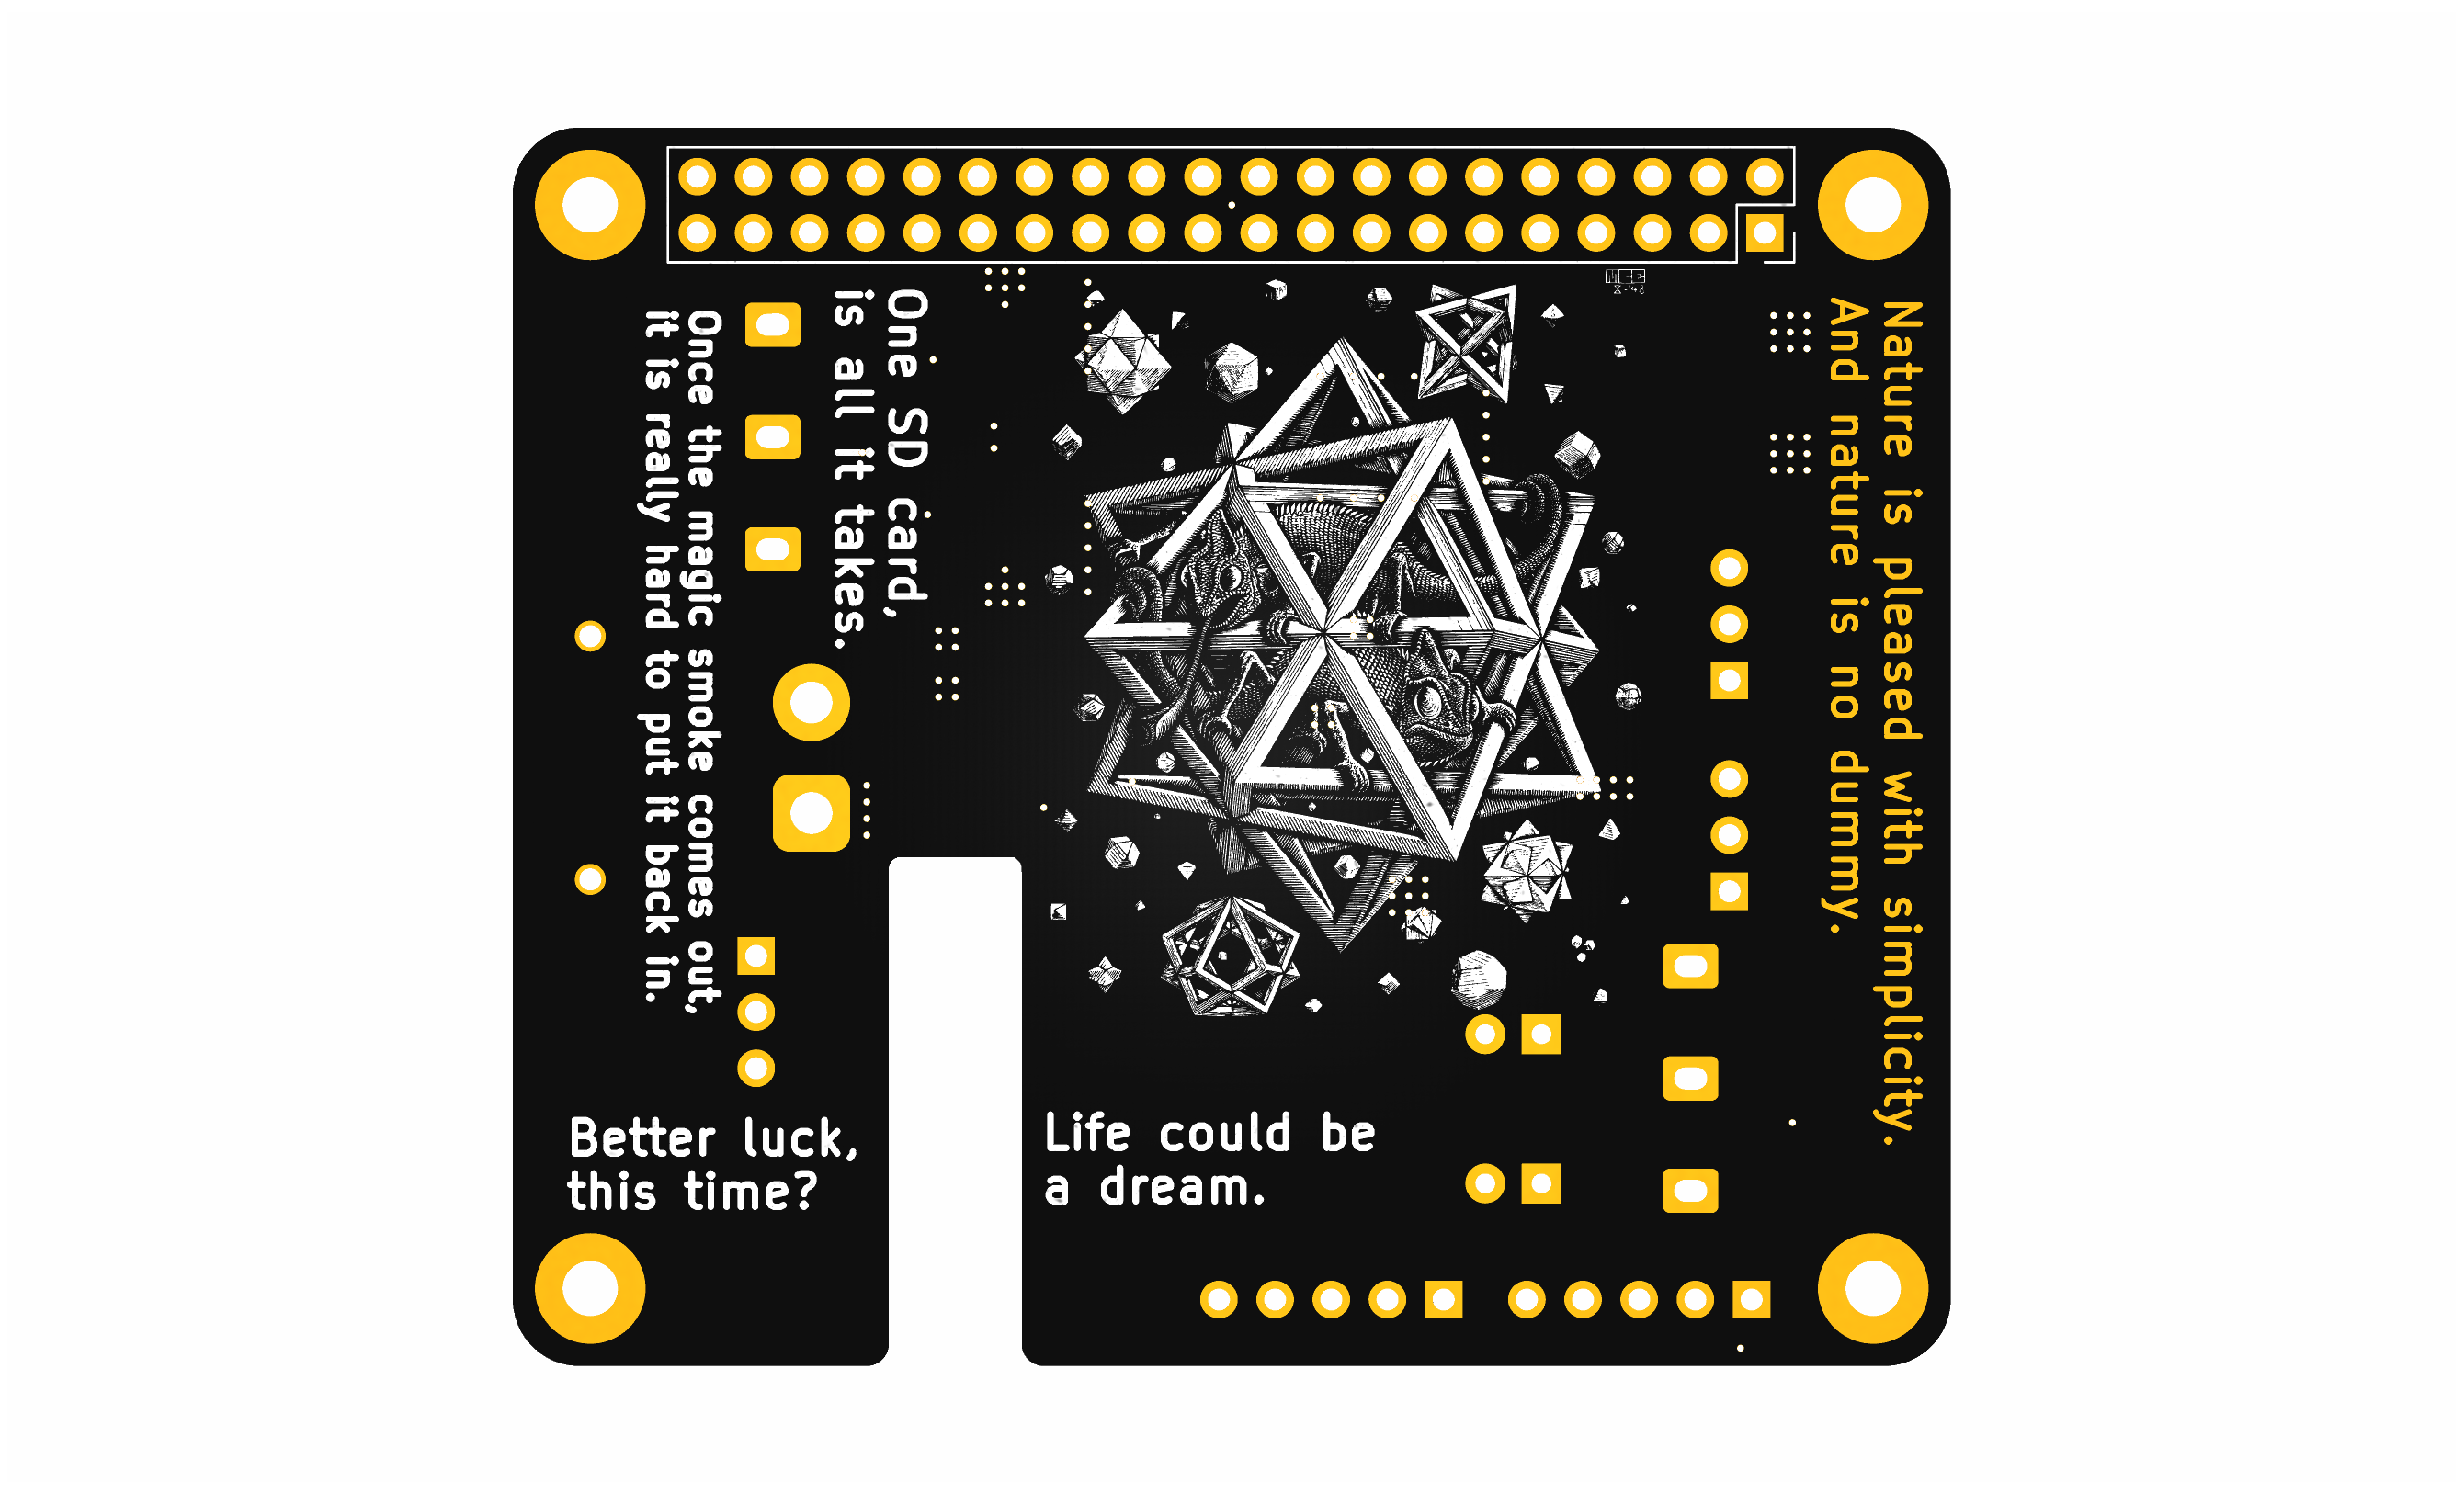
\includegraphics[width=1\textwidth]{img/bottom_render.png}
    \caption{The rendered PCB.}
    \label{fig:KiCAD_Render} 
\end{figure}

The PCB was manufactured by JLC. JLC was chosen due to their lower cost for black solder mask compared to Indian manufactures. The following are the basic parameters:

\begin{enumerate}
\item Base material: FR4
\item PCB Thickness: $1.6$mm
\item PCB Color: Black
\item Silkscreen: White
\item Material Type: FR4 TG135
\item Surface Finish: Lead Free HASL (Hot air solder leveling)
\end{enumerate}

\subsection{Assembly}

The assembly was done by hand. 0603 class components are not too hard to place by hand. Alternatively, assembly can be done by the manufacturer as well. \\

A stencil was used to apply the layer of $183^\circ$ C solder paste on to the board with the help of an old credit card. The "Interactive Html Bom" plugin (Figure \ref{fig:IHBT}) was used to aid with assembly. The plugin creates a interactive html file that can be used to figure out the placement of the components. Alternatively, the PCB and schematic editor can itself be used to figure the placement out but using the plugin is recommended do to its convenience. Once the components have been laid out, a final visual inspection can be carried out. \\

\begin{figure}[H]
    \centering
    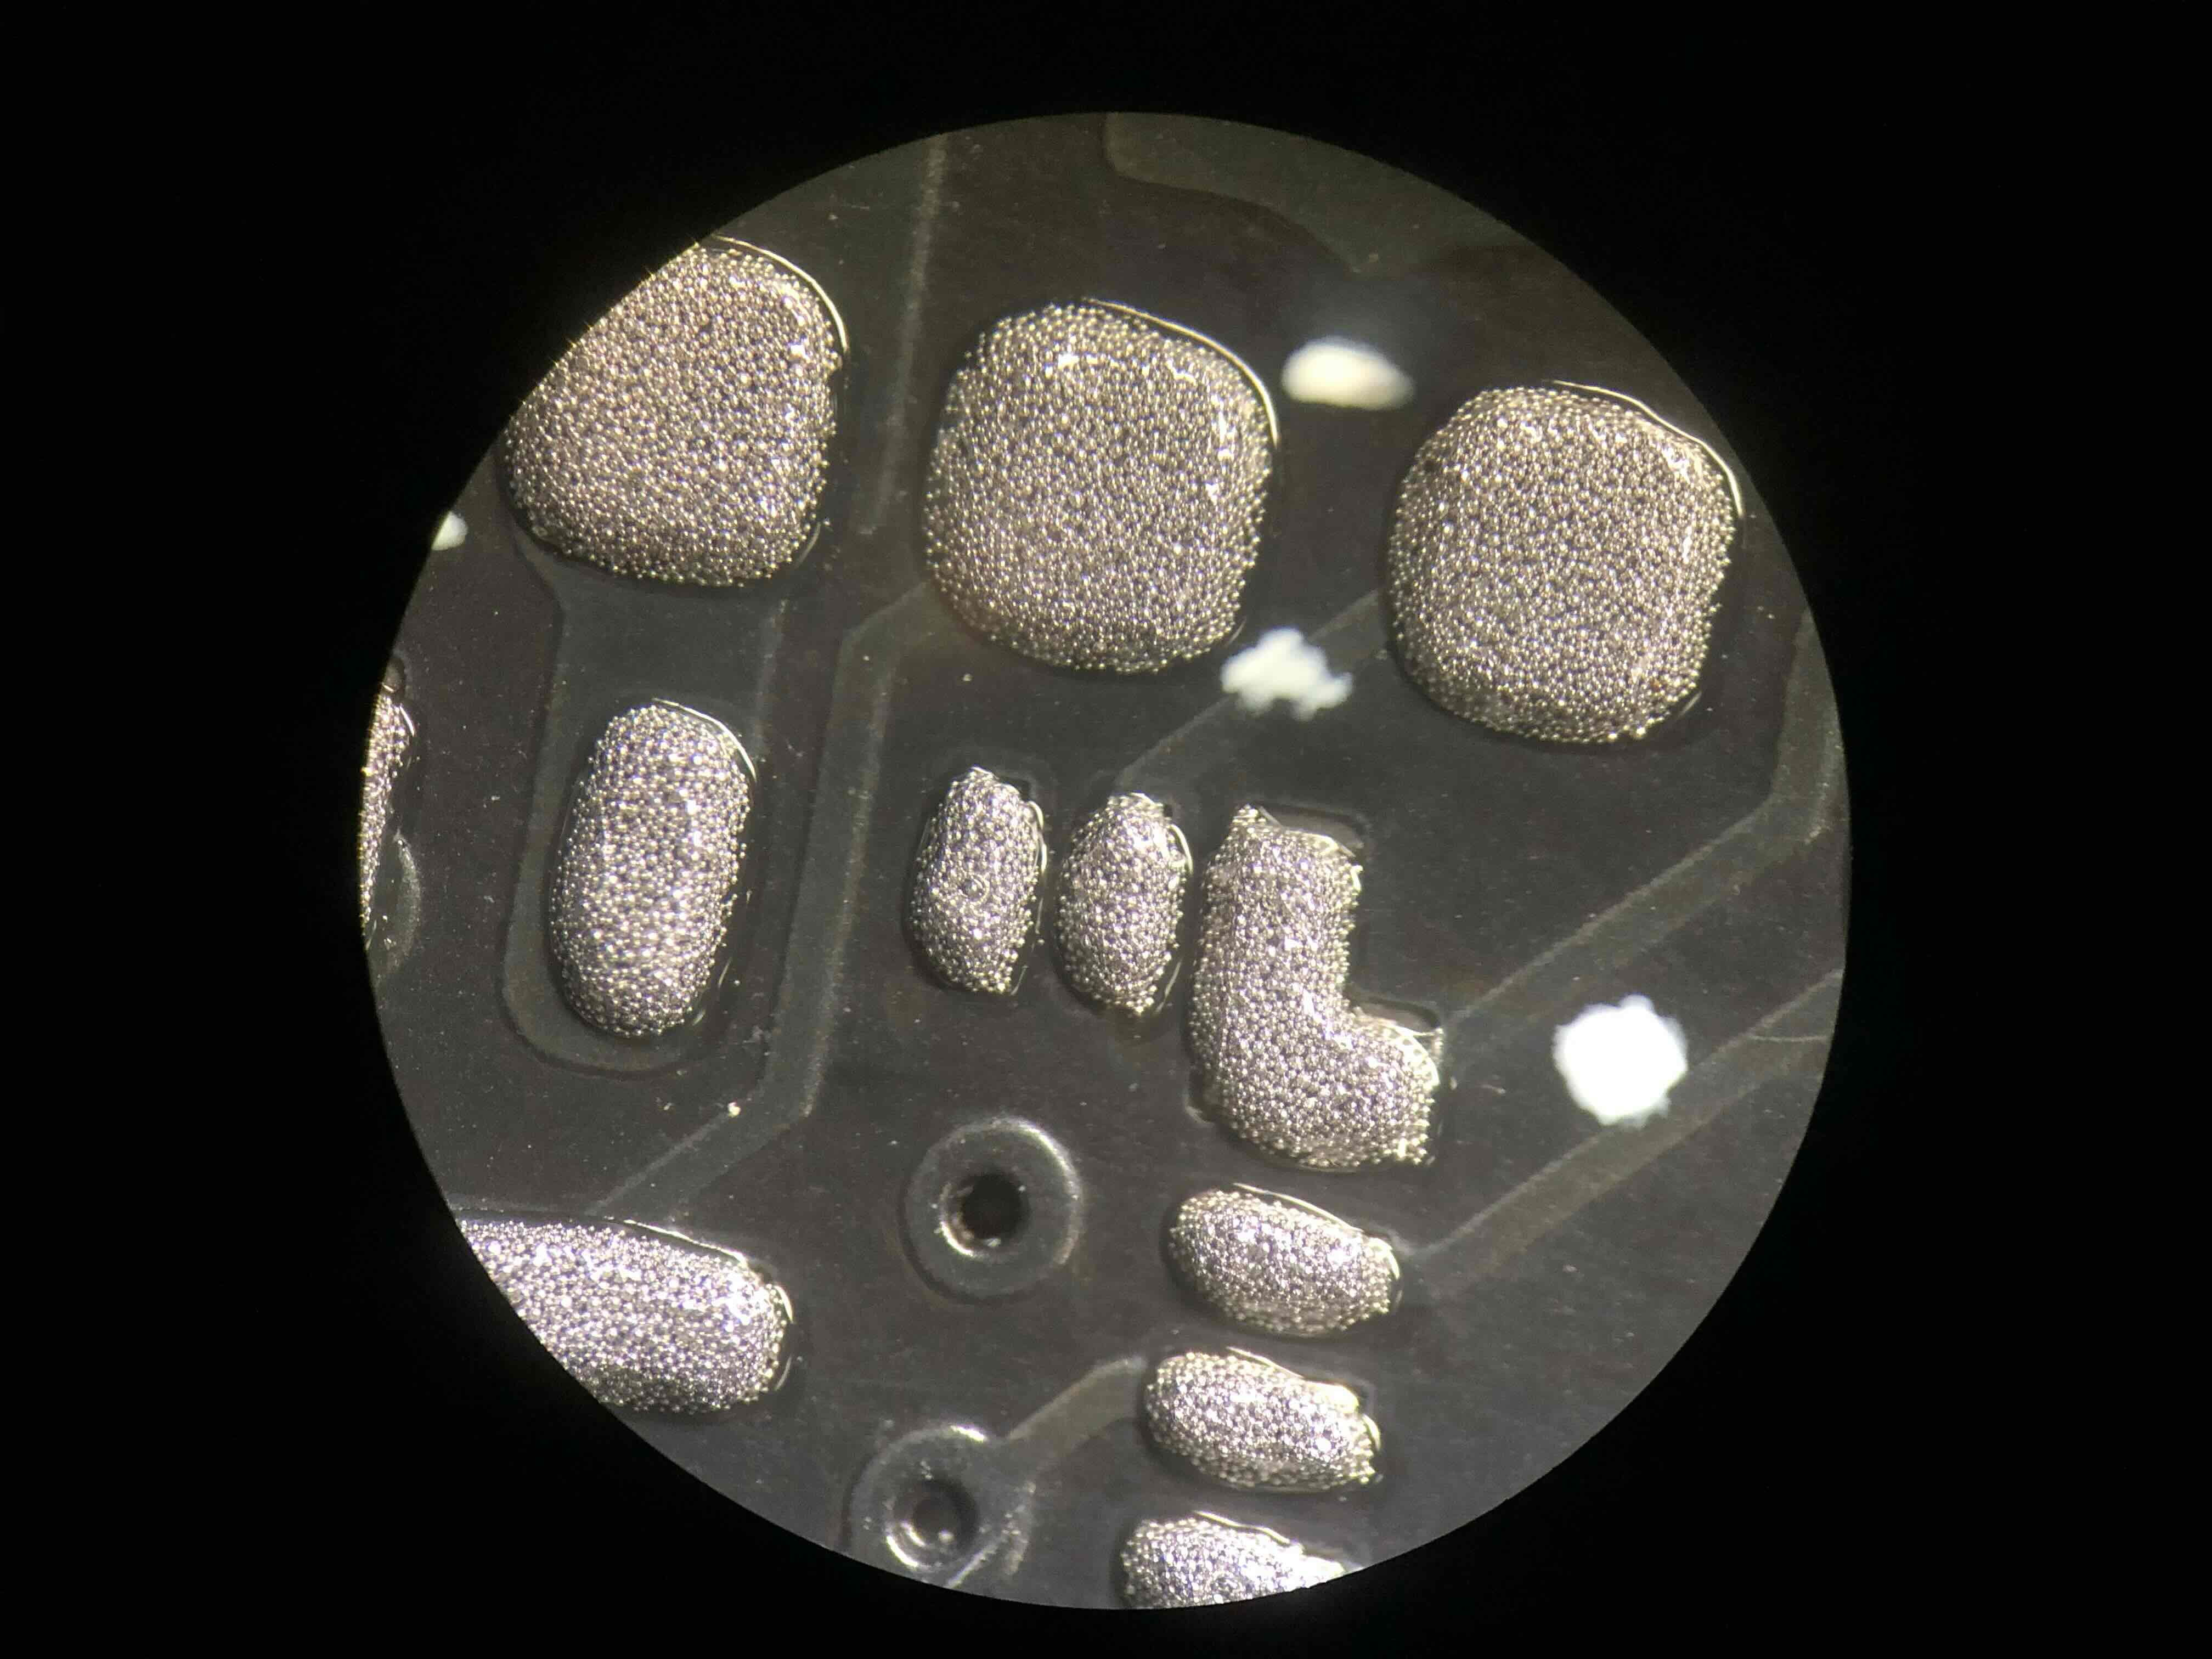
\includegraphics[width=.8\textwidth]{img/solder_paste.jpeg}
    \caption{The solder paste on the pads after being applied with a stencil.}
    \label{fig:solder_paste} 
\end{figure}

The boards can then be re-flowed on the hot plate. It is recommended to follow the heat curve of the solder paste being used. If the plate available does not have the ability to follow a curve, let the board heat soak at about $50$-$80^\circ$ C below the melting point of the solder paste for about 1-2 minutes to let the flux activate before increasing the temperature to its final point. \\

Our hot plate did not have the feature to follow the heat curve so we let our boards soak at $130^\circ$ C for 90 seconds after increasing the temperature to $195^\circ$ C till all of the paste re-flowed and waited 30 seconds more before taking the boards off the hot plate. 

\begin{figure}[H]
    \centering
    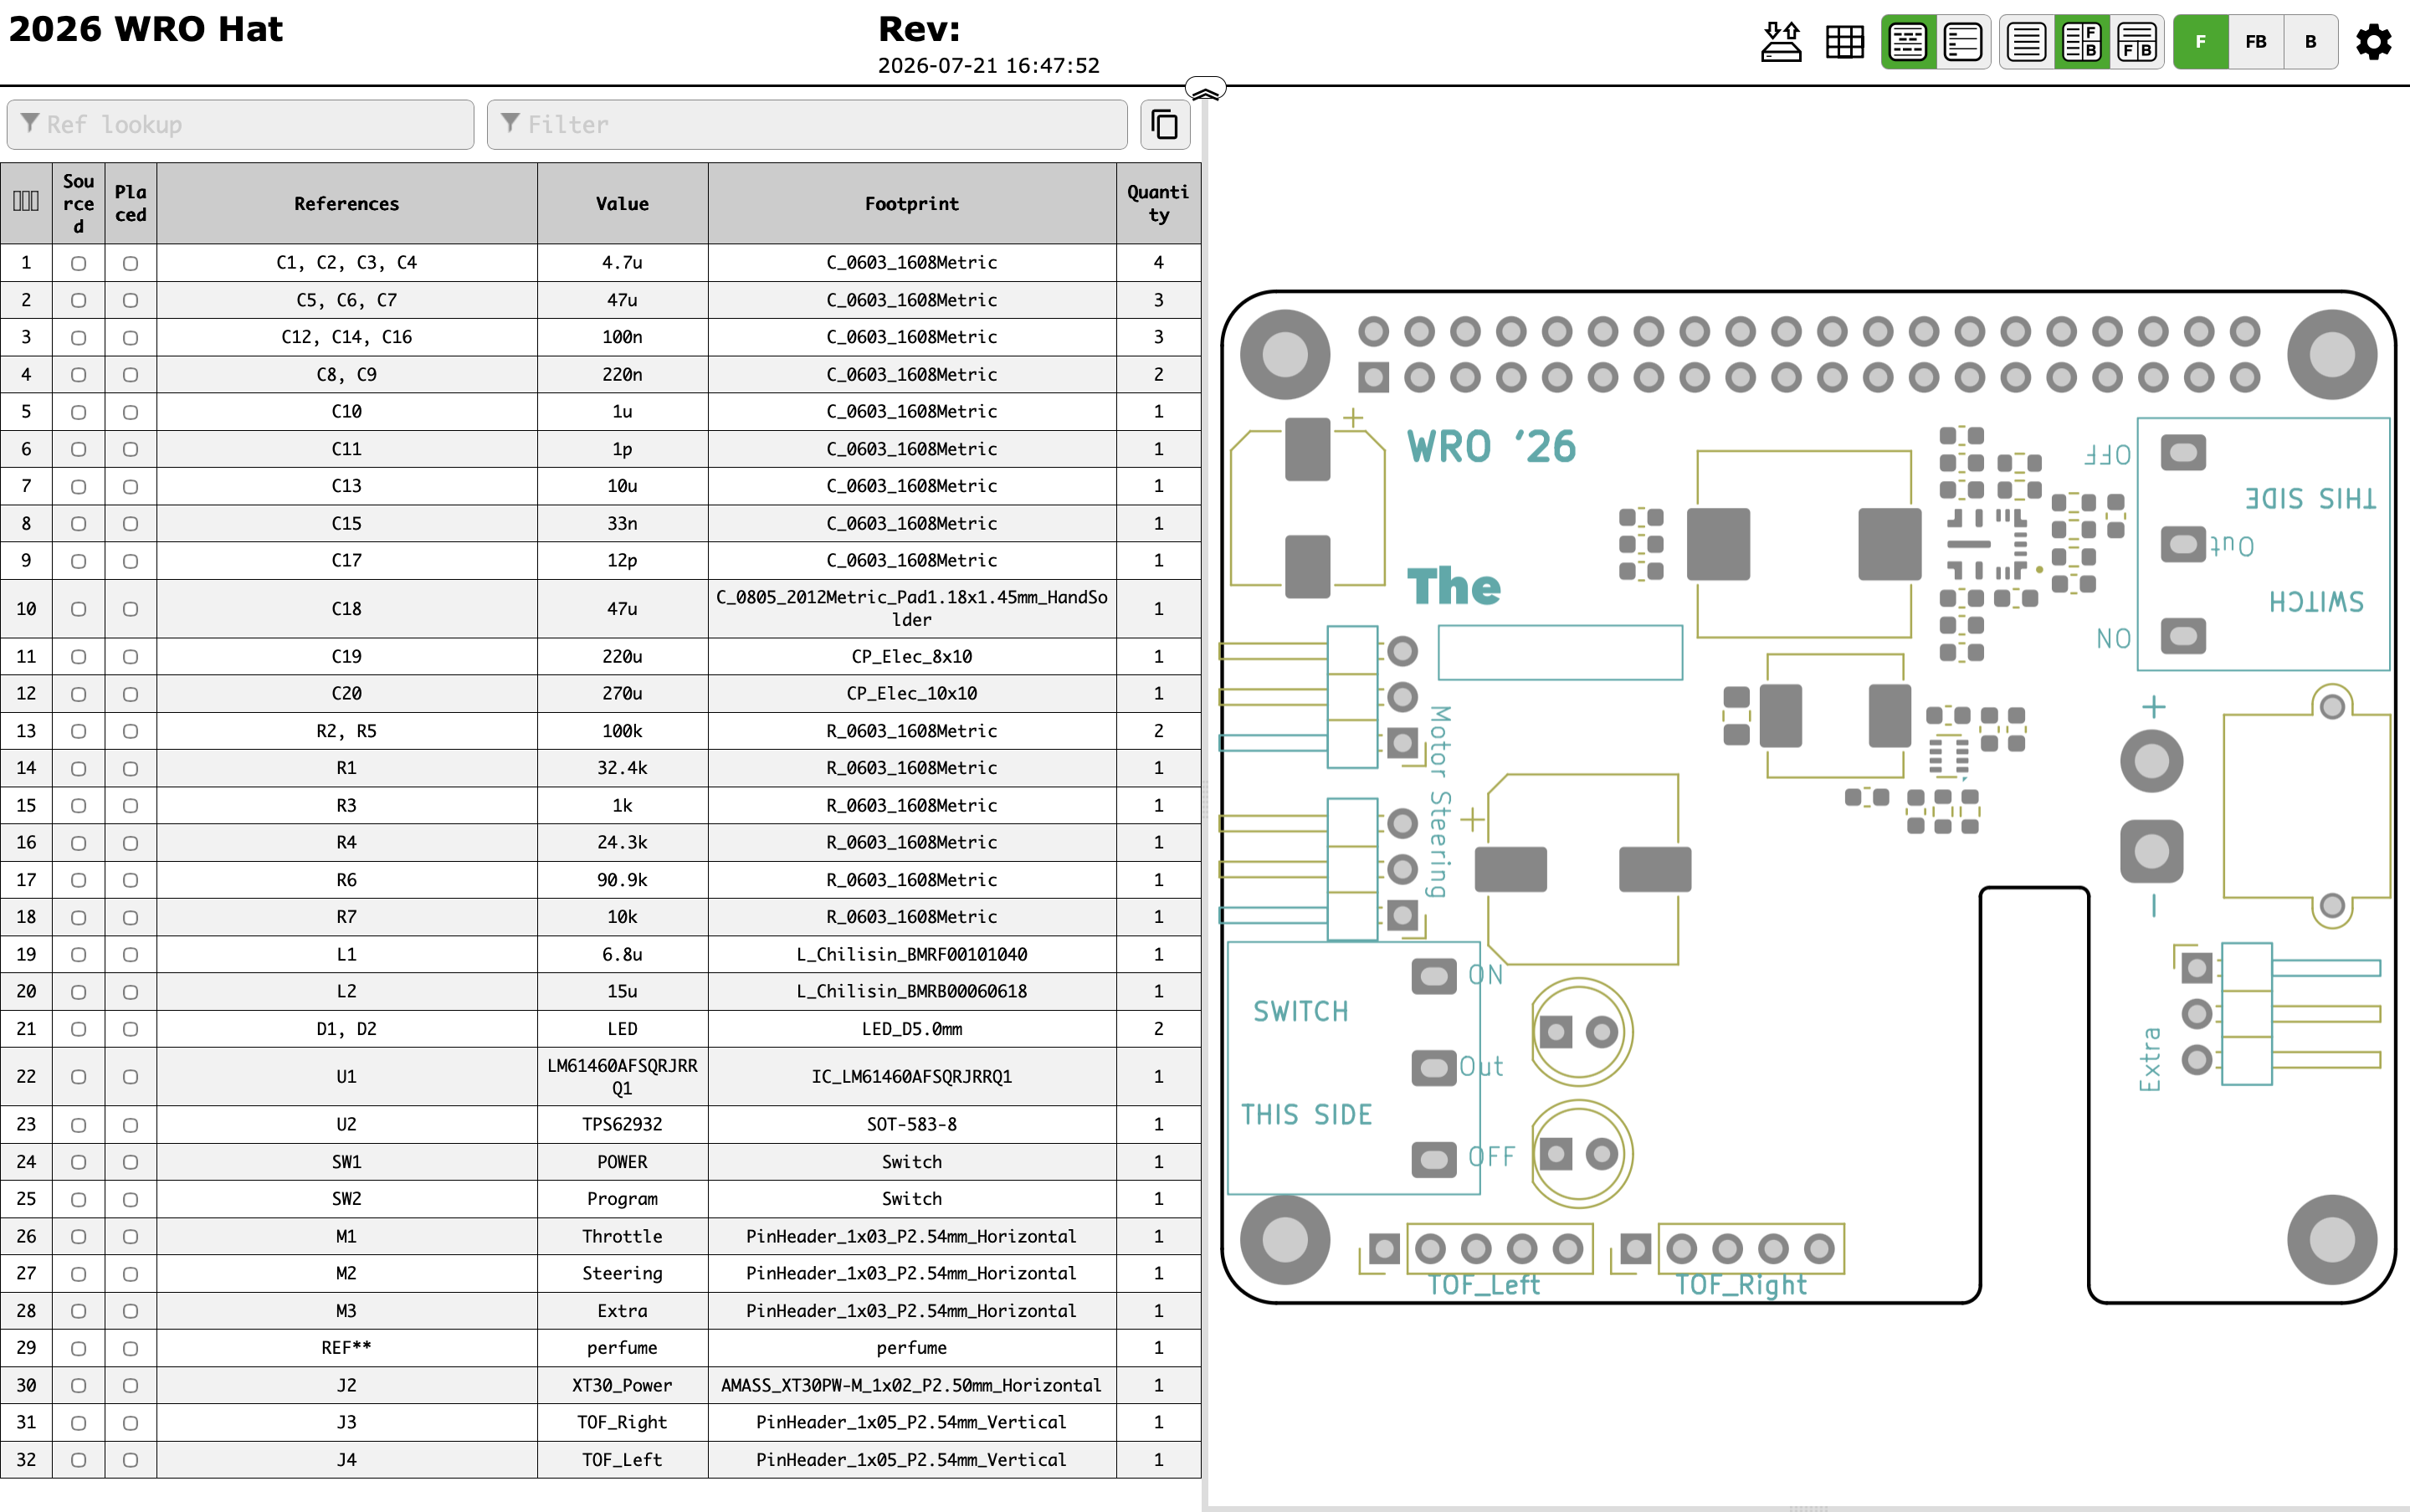
\includegraphics[width=.8\textwidth]{img/IHBT.png}
    \caption{The Interactive HTML BOM Tool.}
    \label{fig:IHBT} 
\end{figure}

The HTML file generated by the plugin can be found in the PCBA folder along with the BOM. \\

Once this is done, the through hole components; like the switches, the power connector and the $20 \times 2$ header connector; can be soldered on to get the final board.  \\

\textbf{Note:} Please refer to the next subsection, Mistakes \& Errors before powering on the board. There is a 1000 $\mu$F capacitor to be added between the output of the switch and GND.

\subsubsection{Advice}

The following is the recommended order for the placement of the components $\Rightarrow$

\begin{enumerate}
\item U1
\item U2 (be careful, some wiggling around is needed)
\item C8, C9
\item C1, C2, C3, C4
\item C5, C6, C7
\item C18
\item R1
\item R2, R5
\item R3
\item R4
\item C10
\item C11
\item C13
\item C12, C14, C16
\item C15
\item C17
\item R7
\item R6
\item L2
\item L1
\item C19
\item C20
\end{enumerate}

\subsection{Mistakes \& Errors}

The first iteration, \textbf{V1.0}, had a fatal flaw. During the schematic design, the enable pin of the LM61460 was connected to ground. The enable pin needs a voltage of greater than about $3$V. This mean that the chip would be in the "shutdown mode". This mean it would not work at all. \\

To attempt fix this issue, the trace from the GND via to the EN pin was cut off using a razor blade. A thin copper wire (32 AWG) was then added very carefully between the VIN and the EN pad. Typically, this is called a "\textbf{bodge}" (Figure \ref{fig:bodge}). This turned out to be very unsuccessful. This was because of the Package of the IC and the microscopic, but still substantial thickness of the wire. The VQFN package has flat pins at the bottom that interface with the surface directly (Figure \ref{fig:LM61460}). This meant that while the wire was fairly thin, its thickness meant that not all the pins of the IC made contact with the PCB. It was sort of like a see saw. Another attempt was made with a thinner strand of wire, about a third of the diameter but that was also unsuccessful. \\

Hence the decision was made to re order a new set with the fixed connections, \textbf{V1.1}. The original error was traced down to a mistake in copying the schematic from TI workbench to the KiCAD schematic editor. \\

\begin{figure}[H]
    \centering
    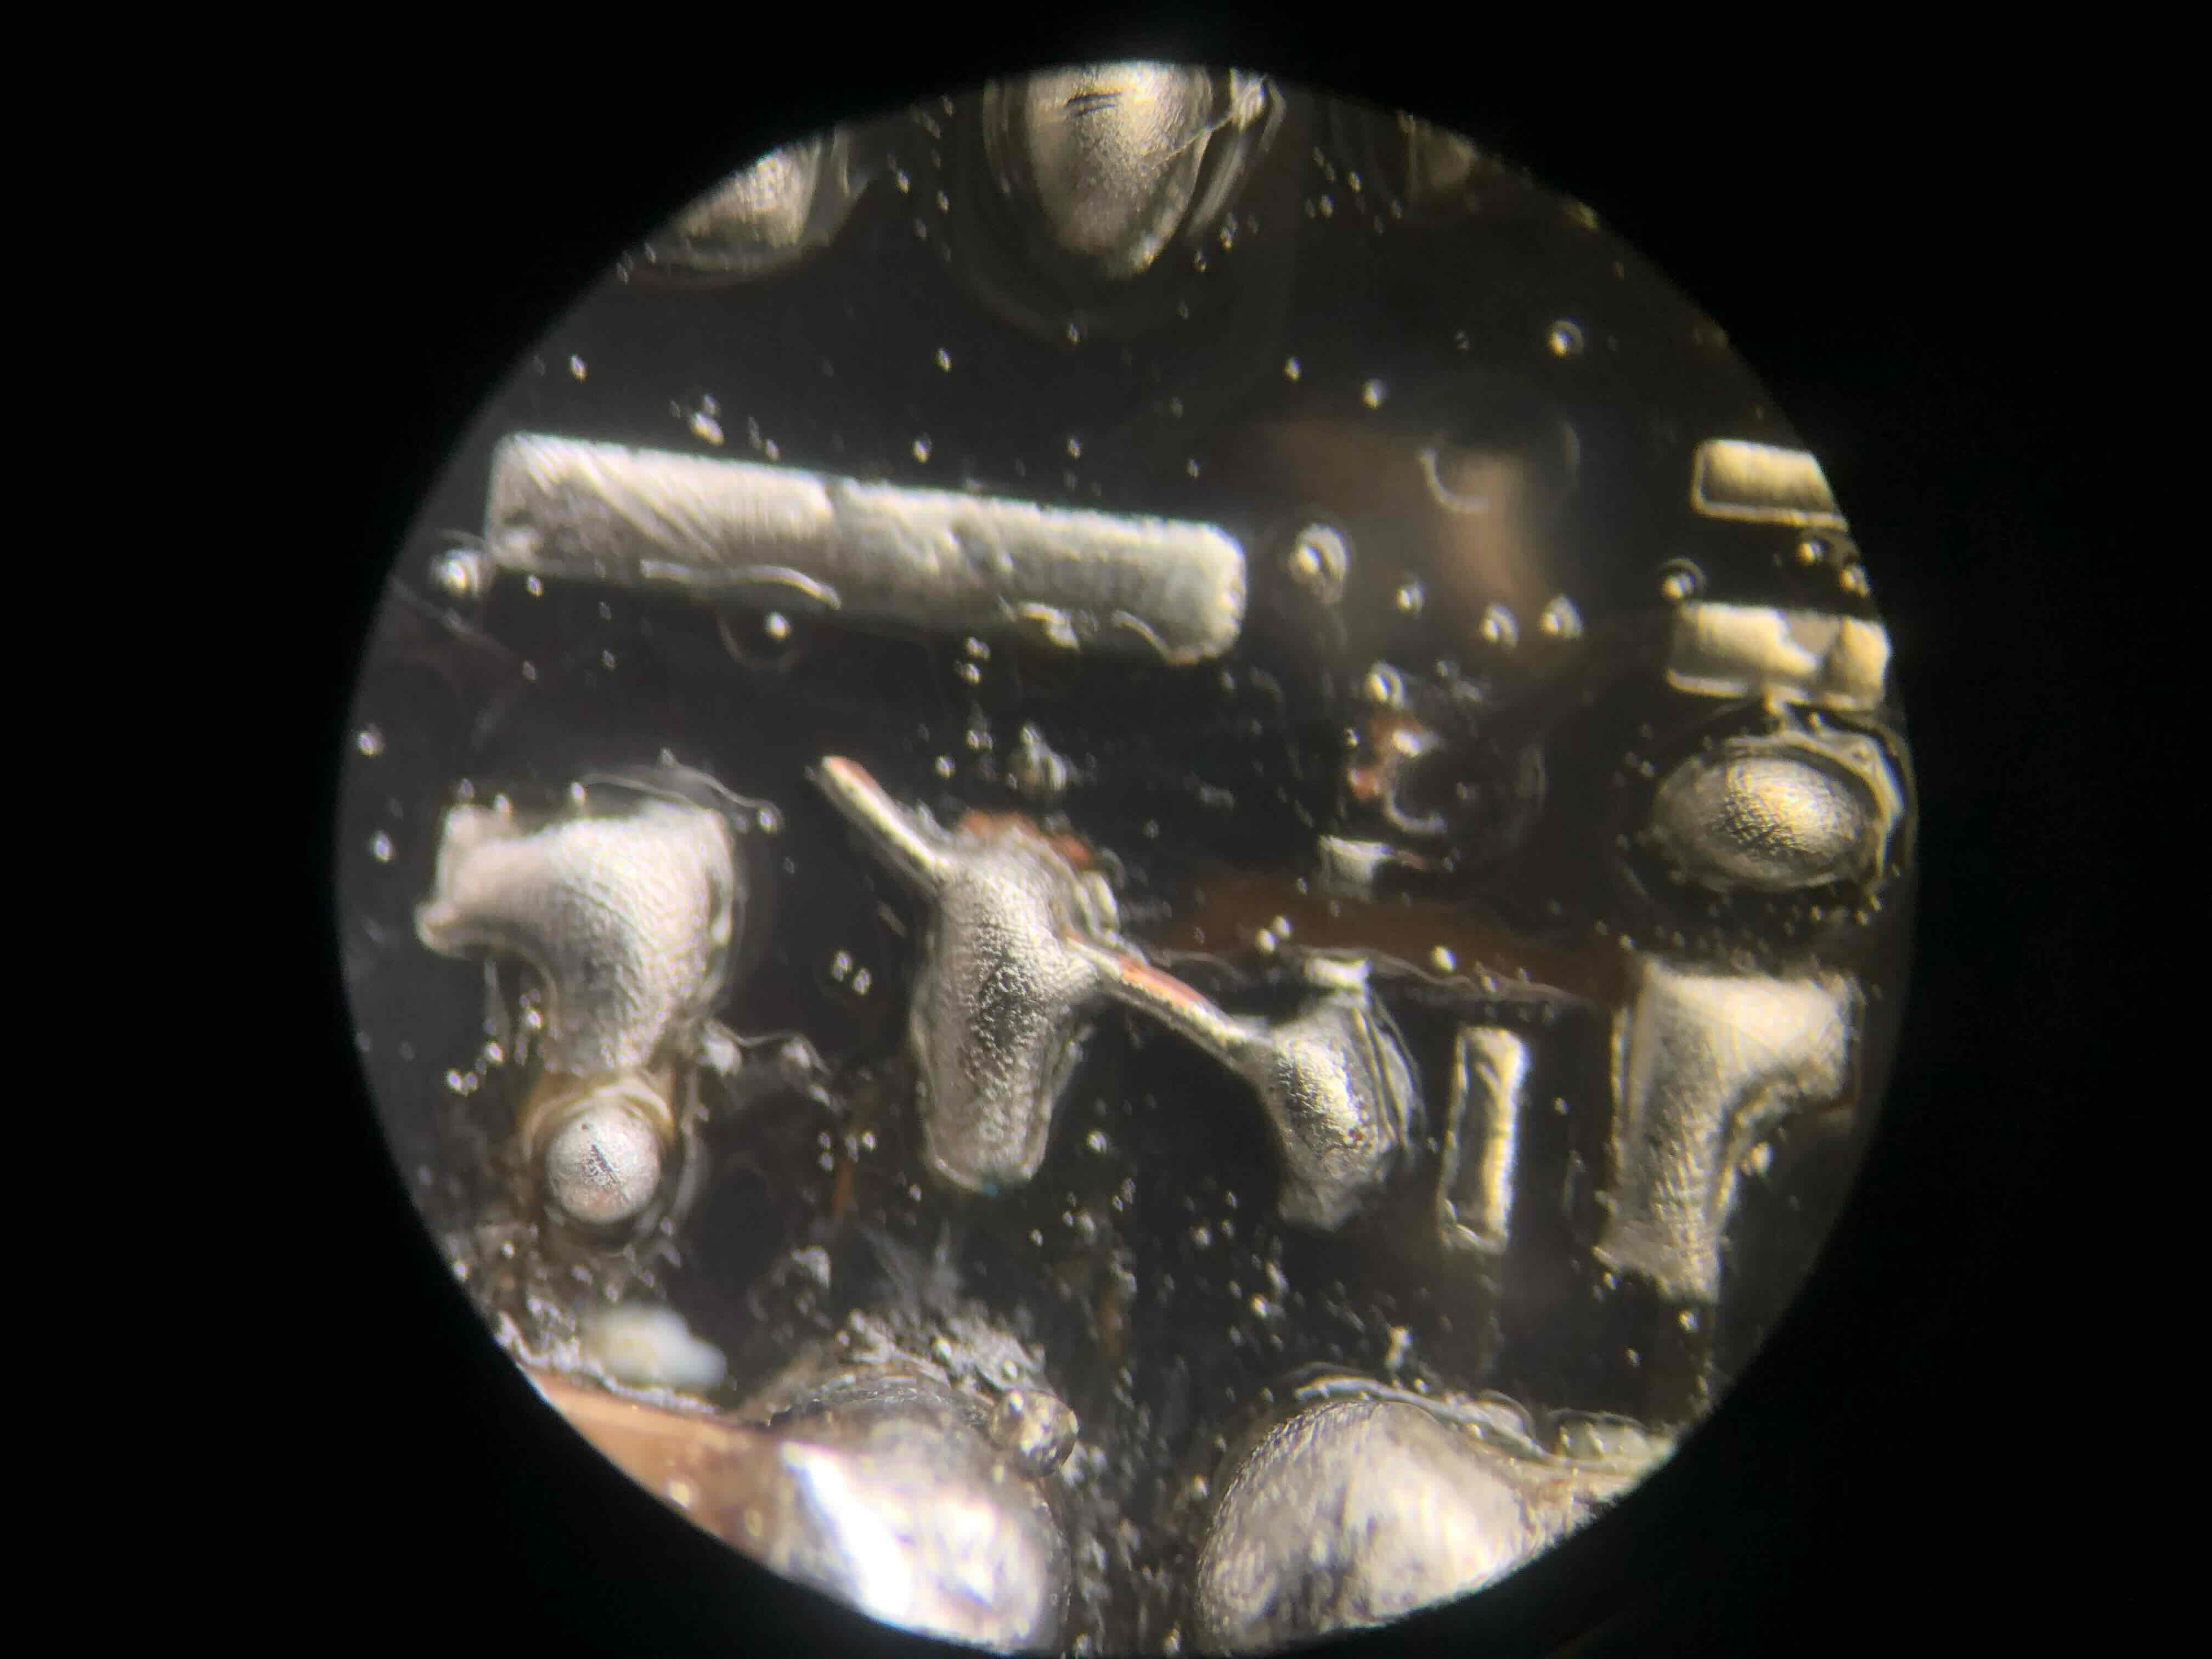
\includegraphics[width=.8\textwidth]{img/bodge.jpeg}
    \caption[The Bodge Wire.]{The brown area on the top right of the copper wire represents the cut out trace.}
    \label{fig:bodge} 
\end{figure}

The newer version, \textbf{V1.1} was assembled successfully and worked flawlessly, providing $5.15$V to the Raspberry Pi as intended. During hardware testing, when using the switch to power on and off the Raspberry Pi, the LM61460 chip, literally, burst into flames and released the magic smoke. This was right as the switch had been toggled to the on position, triggering a catastrophic hardware phenomenon known as an LC hot-plug transient spike. The wires from the battery inherently act as an inductor, and the ultra-low ESR (Equivalent Series Resistance) ceramic input capacitors on the board act as a capacitor, together forming an undamped LC resonant circuit. When the mechanical switch was flipped, its internal contacts bounced microscopically. This rapid connect-disconnect action, combined with the near-zero resistance of the ceramic capacitors, caused the sudden inrush current to ring like a bell. The voltage overshot significantly, effectively doubling the 16.8V battery input and easily punching through the 36V absolute maximum rating of the LM61460. \\

This destructive spike was further amplified by the DC bias derating of the ceramic capacitors, which temporarily lose capacitance under high voltage, forcing the transient spike even higher. The fix for this required introducing a "shock absorber" to dampen the resonant circuit. By adding a 1000 $\mu$F electrolytic capacitor directly between the output of the switch and ground, the naturally higher ESR of the electrolytic component safely dissipated the kinetic energy of the inrush current as microscopic heat. This completely arrested the pendulum swing of the LC ringing, clamping the voltage safely to the battery level and bulletproofing the circuit against future switch bouncing. \\

\textbf{NOTE:} The PCB design files do not include this fix, and it is to be implemented after.

\pagebreak

\section{3D Prints \& CAD}

The body of the vehicle is primarily made up of 3D printed parts. Onshape was the CAD package used. Extreme considerations were made when designing the vehicle. Ease of reputability, along with structural rigidity were the utmost priority when designing the parts. This was exasperate from the constraints already present when using FDM (Fused Deposition Modeling) 3D printing. \\

Tolerances for the parts were borrowed where ever possible as a foundational design principle to ensure predictable and consistent assembly. Because FDM printing is inherently prone to dimensional variations; caused by thermal shrinkage, layer lines, and extrusion inconsistencies; calculating unique clearances for every single joint is highly inefficient and risks assembly failure. \\

By standardizing and "borrowing" proven tolerance profiles (such as a baseline $0.2$mm gap for slip fits and $0.4$mm for clearance holes) across the entire CAD model, the design creates a modular, standardized system. This strategic allocation allows non-critical dimensions to absorb the printer's inherent inaccuracies. Ultimately, this prevents tolerance stack-up issues and guarantees that structural interfaces bolt or snap together seamlessly on the first print, eliminating the need for tedious manual post-processing, filing, or reprint iterations. \\

Pre-flight and Orca Slicer were the Slicers used for the conversion of the 3D files into G-Code. The utmost care was given to the parts in the design process. There are no large parts that need a massive printer to be printed. All the parts can fit on a minimum build volume of about $150 \times 150 \times 150$ mm. The whole assembly was created in Onshape to ensure parts fit together seamlessly. \\

\subsection{Layout \& Wheelbase}

To adhere to the strict volume limitations we set in the introduction, a slightly wider wheelbase was opted compared to what most competitors would probably use. This was done so that more horizontal volume could be allotted to the components without shifting them vertically. A strict horizontal width limit was put at $180$mm to ensure the $200$mm limit was not breached. The wheels where placed as far out as possible to maximize component volume and have better stability. \\

A wheelbase of $184.3$mm was chosen. A longer wheelbase would mean that the vehicle would have trouble parallel parking. The number $184.3$, may seem odd but it was derived from scaling the Aston Martin Valkyrie down to the size of the wheels being used. \\

The layout, as mentioned earlier, a Rear Wheel drive mechanism with front wheel steering was chosen. This made the layout slightly easier but it was crammed nevertheless. Figure \ref{fig:Top_main_view} shows the CAD assembly, moving top down. \\

\begin{figure}[H]
    \centering
    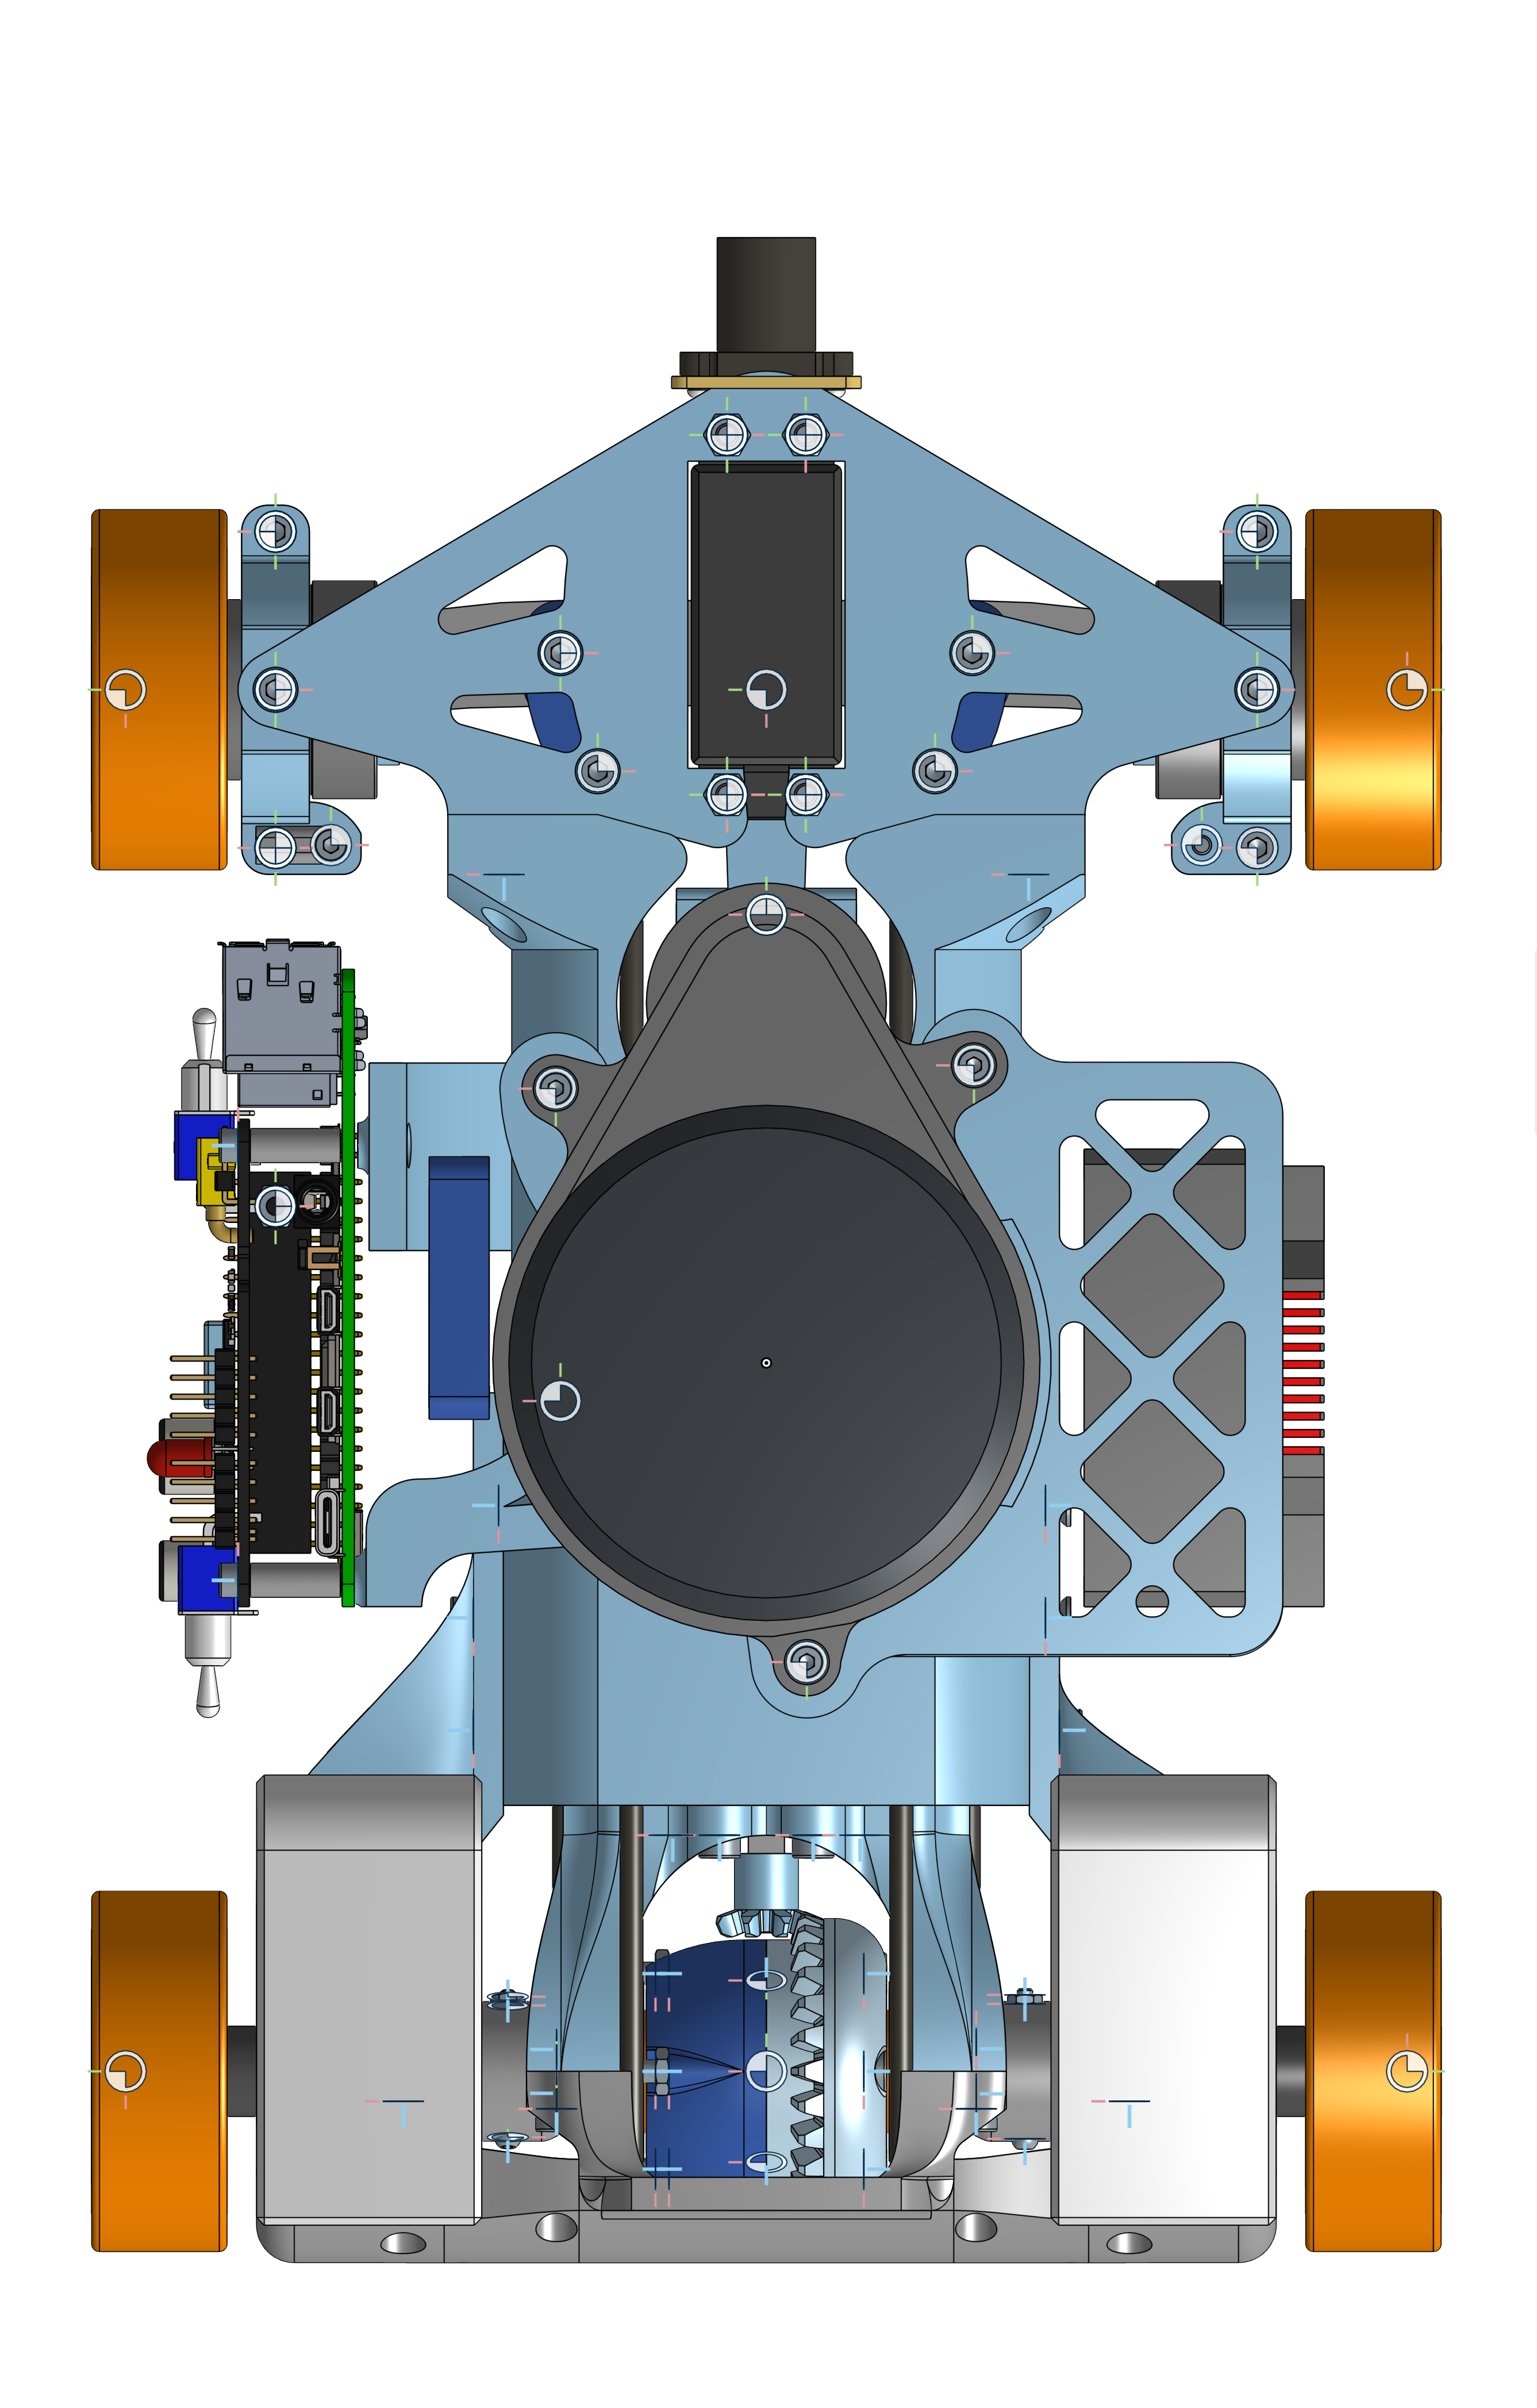
\includegraphics[width=.8\textwidth]{img/top_full.png}
    \caption{The Onshape assembly.}
    \label{fig:Top_main_view} 
\end{figure}

Starting at the front, we have the camera as the front most element. This is driven by the fact that the camera has a very high FOV and the best view would be unobstructed. Just behind it is the front axle. It houses the steering system and the bearings. In the center there sits the LiDAR, directly positioned on top of all the components. Below the LiDAR, with a healthy amount of spacing to prevent EMI is the motor. To the right of the motor, the ESC is mounted vertically. The Raspberry Pi is mounted on the left side of the motor. Moving further back, we reach the differential and the rear axle. The batteries sit atop the rear axle baring mounts. \\

It was critical for every single part to be accounted for. All the models were self designed. There are a few critical assemblies that need to be discussed in order. \\

\subsection{The Steering Assembly}

\subsubsection*{Front Wheel Adapter}

The steering assembly originates from two points in space, the contact points for the needle roller thrust bearings (Figure \ref{fig:needle_roller_thrust_bearing}). The bearings connect to the wheels via a rod that is capped at on end. The rod as a nominal diameter of $12$mm and a length of $38$mm. The cap at the end has a diameter of $20$mm and a width of $3$mm. The rod also has a $\diameter 2$mm hole at the end, spaced $4.5$mm from the edge of the non capped end to interface with the wheel (Figure: \ref{fig:wheel_CAD}) via a M2 screw.

\begin{figure}[H]
    \centering
    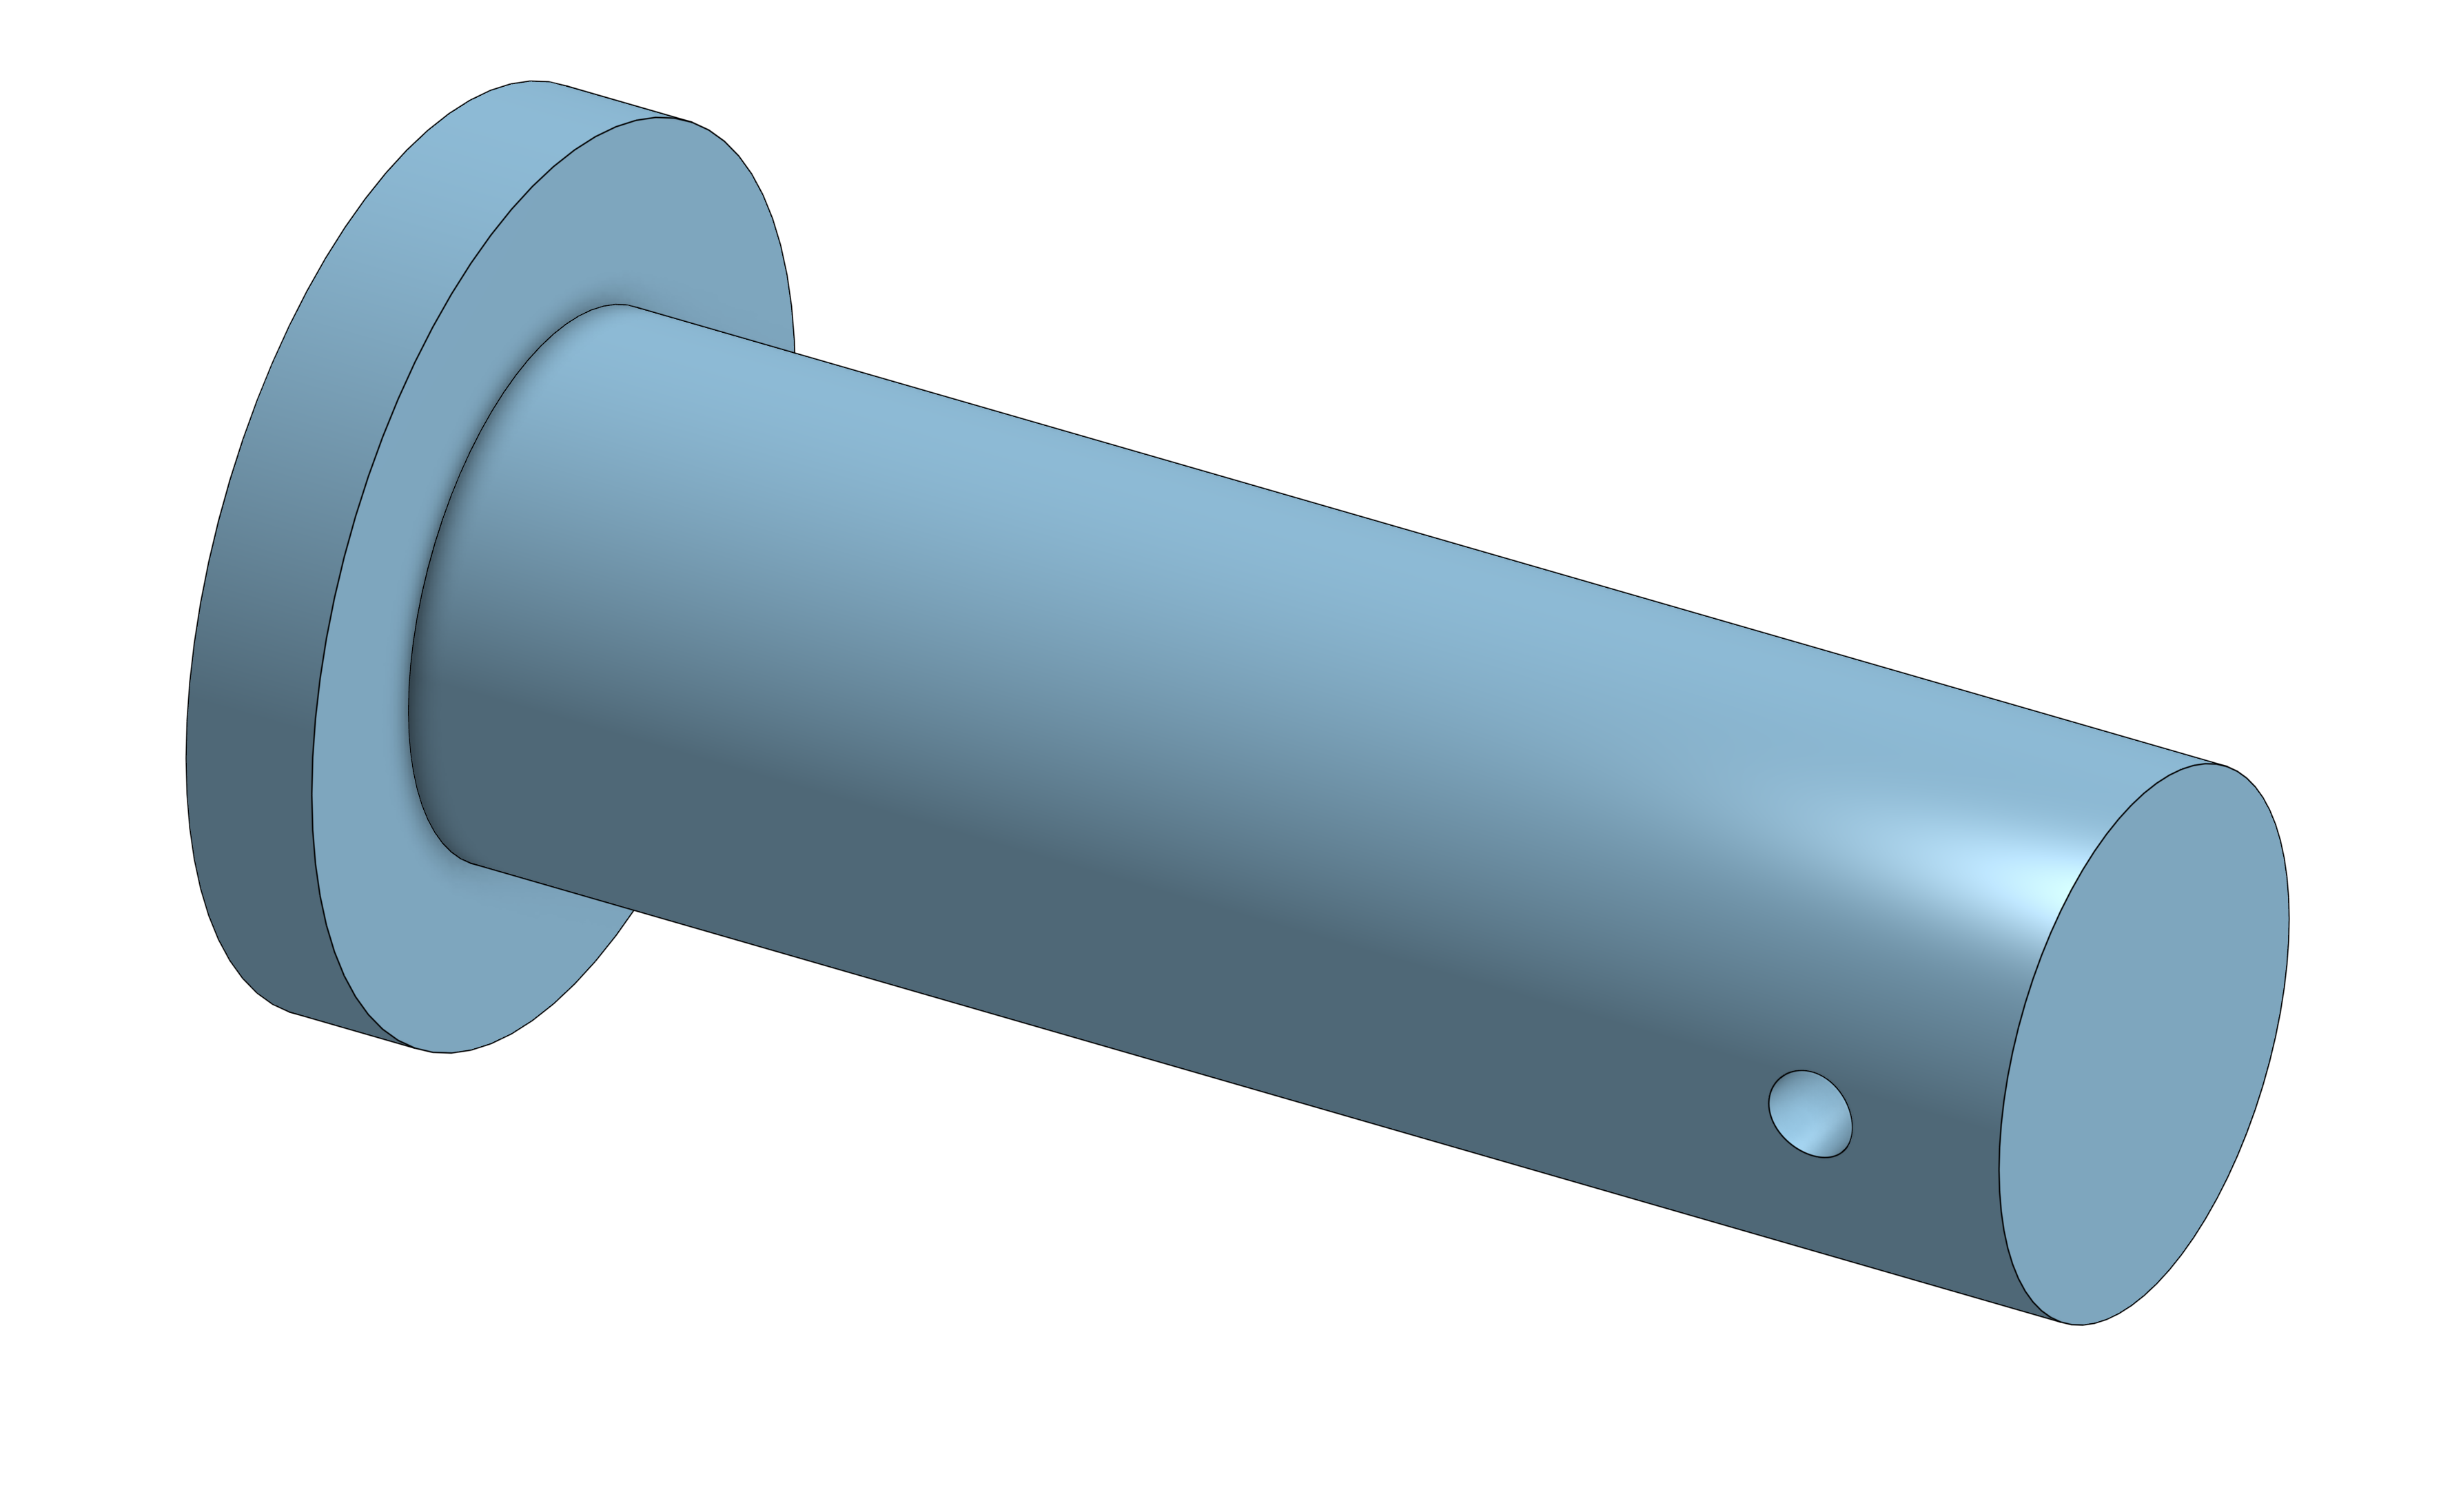
\includegraphics[width=.4\textwidth]{img/front_wheel_adapter.png}
    \caption{The Front Wheel Adapter Pin.}
    \label{fig:C_FWA_pin} 
\end{figure}

The pin is printed vertically, with the cap end facing down. This does spread the load across the layer lines, the load on the front wheels isn't drastic enough for one to be concerned. The part is printed with a layer height of $0.2$mm, has $3$ perimeters and a $25\%$ infill.

\subsubsection*{Steering Knuckles}

We next interface with the stationary parts of the bearing. To do this, we make a clamp style part that relies on the pressure and friction to keep the bearing constrained. We replicate the grove in the bearing as a positive feature to constrain the bearing axially.\\

\begin{figure}[H]
    \centering
    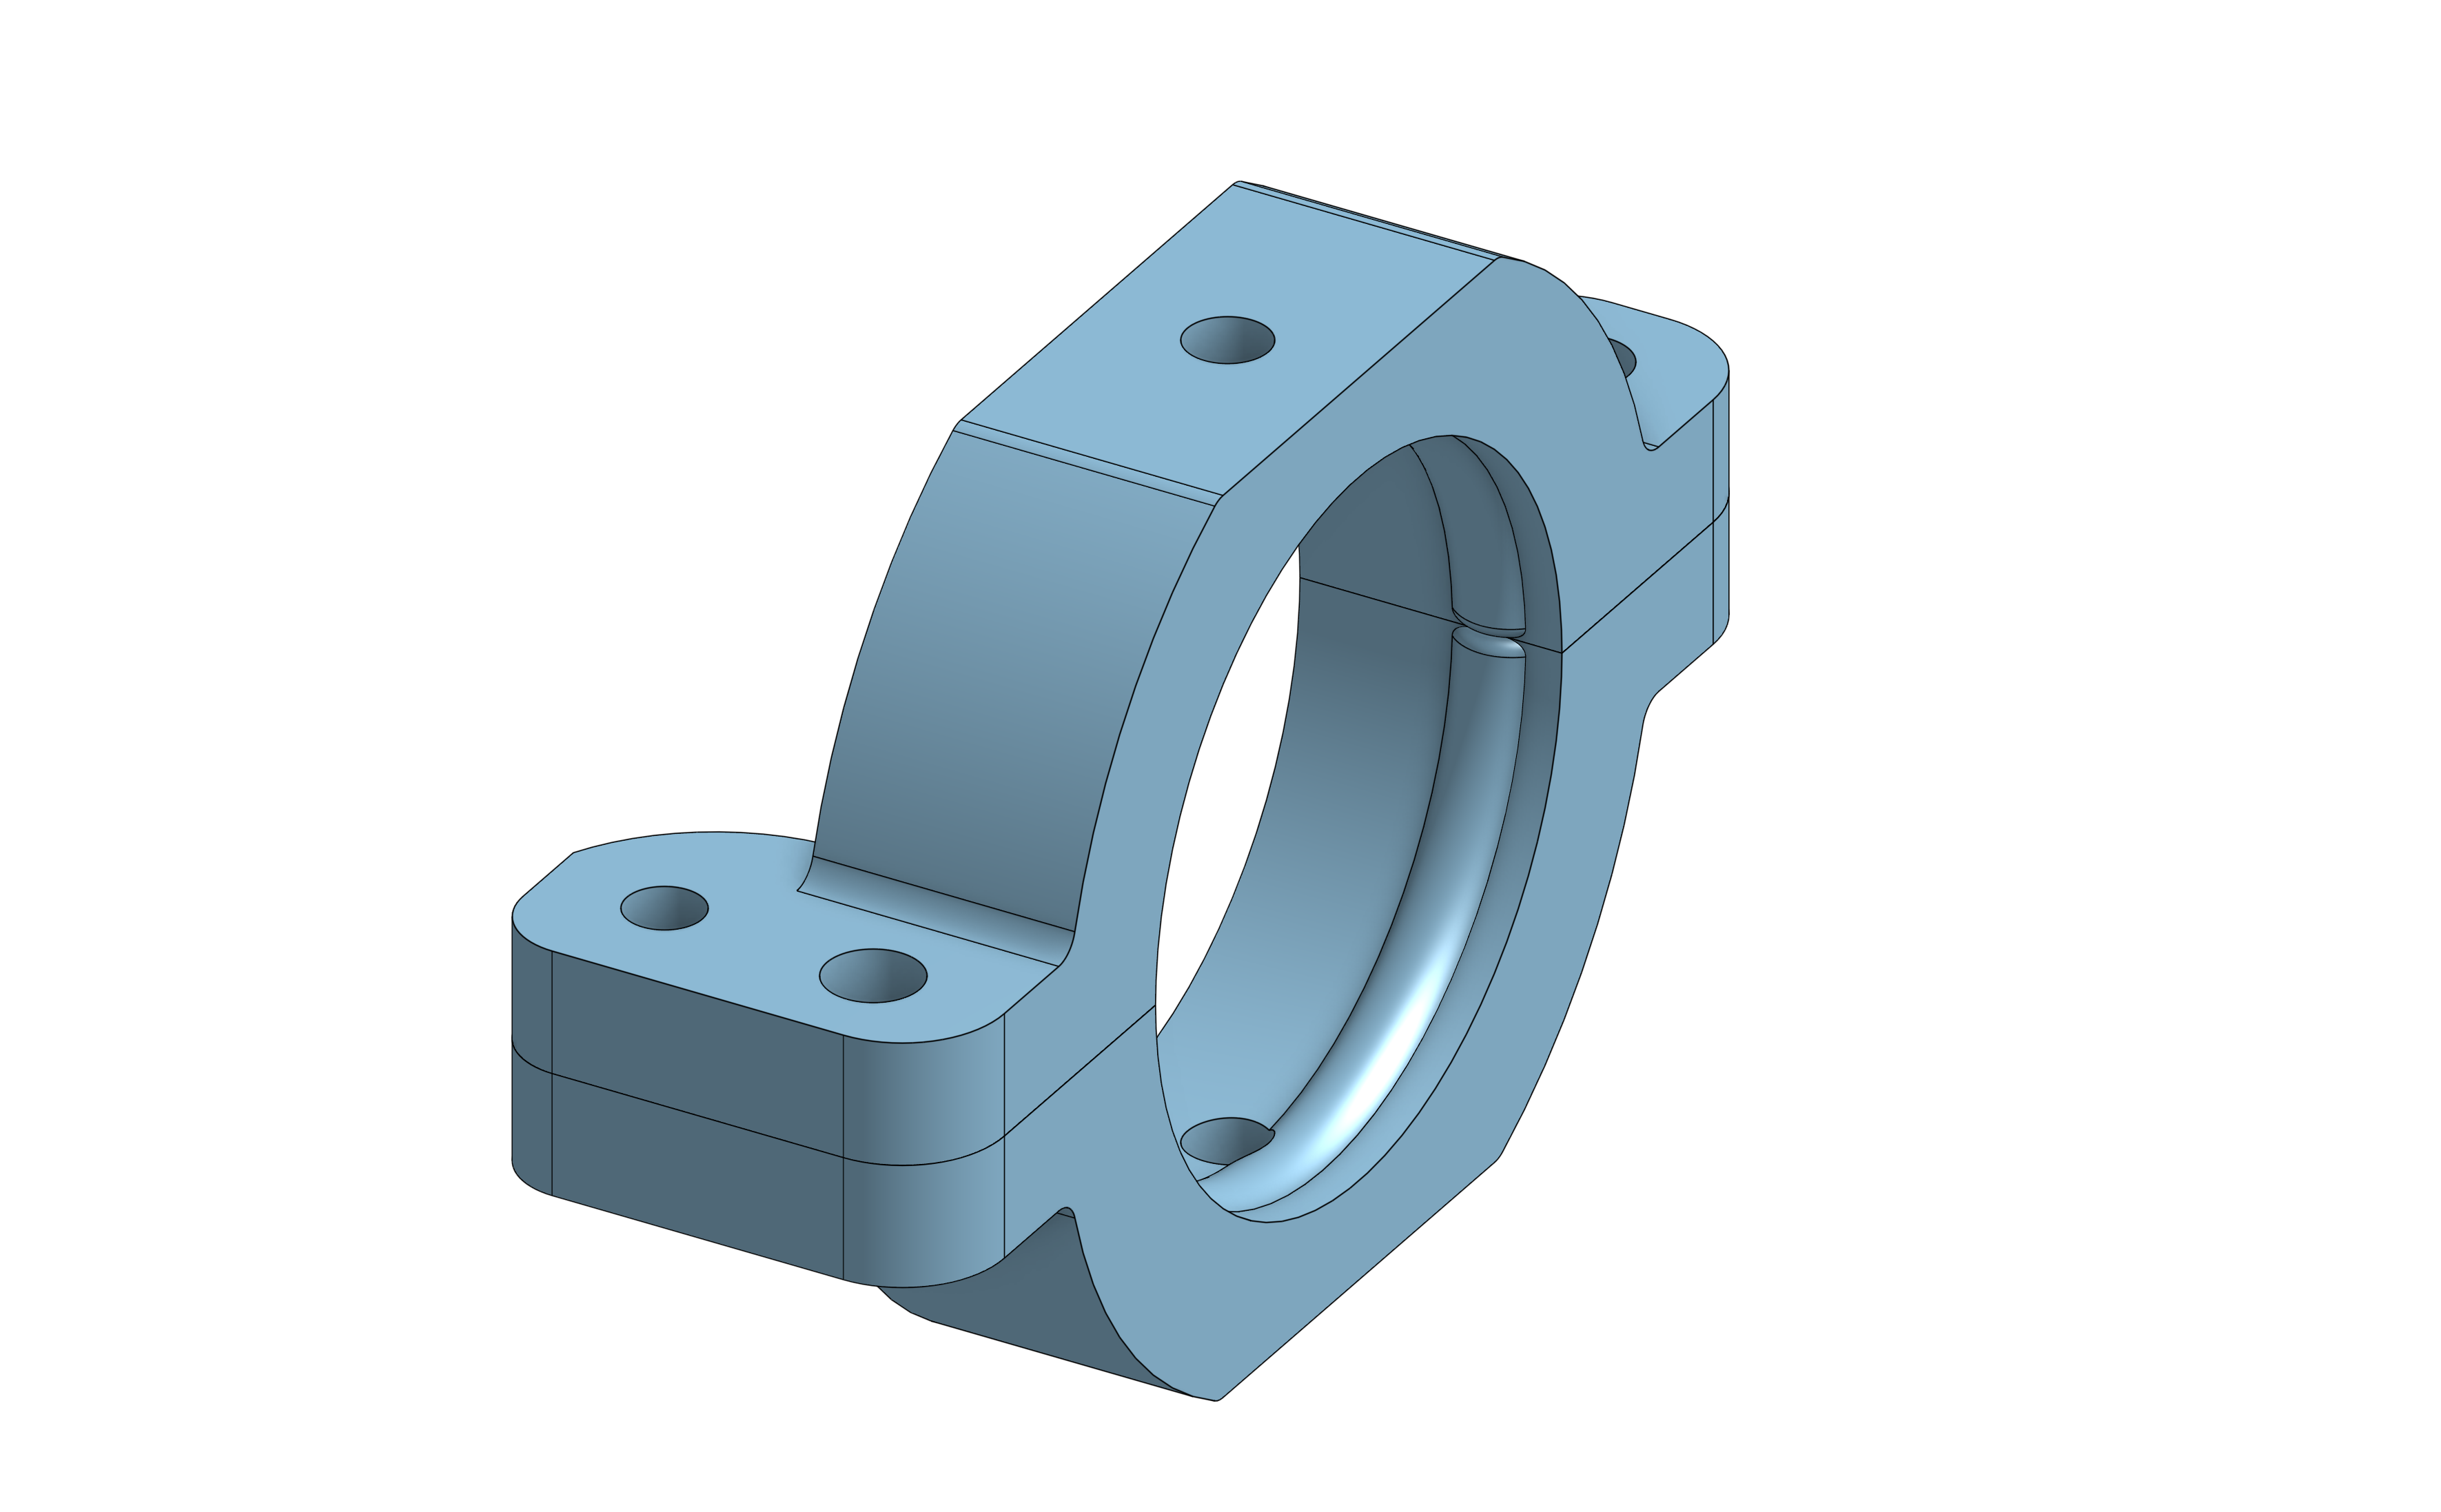
\includegraphics[width=.4\textwidth]{img/steering_knuckle.png}
    \caption{The Steering Knuckle.}
    \label{fig:C_SK} 
\end{figure}

To interface the two part clamp, we use two M$3 \times 12$ screws and M$3$ nuts. We flatten out the sphere at $\diameter 31$mm so that the clamps can interface with the other steering parts and rotate in the vertical axis. To do this, we add a $\diameter 2.8$mm hole on the top for a M$3$ screw. We keep the hole smaller than the screw diameter so that the screw can create the threads in the plastic part as it enters. This is done as using a heat set inset would take too much space. Also it is justified by the lower loads. We also add a $\diameter 2.5$mm hole so that a screw can be added for the steering rod interface. These would be like Steering Knuckles in a traditional car. It is mirrored to fit on the left side. \\

The part is printed with the face closest to the bearing (and image in Figure \ref{fig:C_SK}) facing down. This not only transfers the loads along the layers but also ensure a good interference fit with the bearing. The part is printed with a layer height of $0.2$mm, has $3$ perimeters and a $25\%$ infill. 

\subsubsection*{Steering Column}

The steering column consists of 4 parts (See Figure \ref{fig:C_SC}), the top brace (light blue), the bottom brace (grey) and 2 side braces (dark blue). It mounts the servo on the center of the front axle and provides interface points with the rest of the vehicle. \\

\begin{figure}[H]
    \centering
    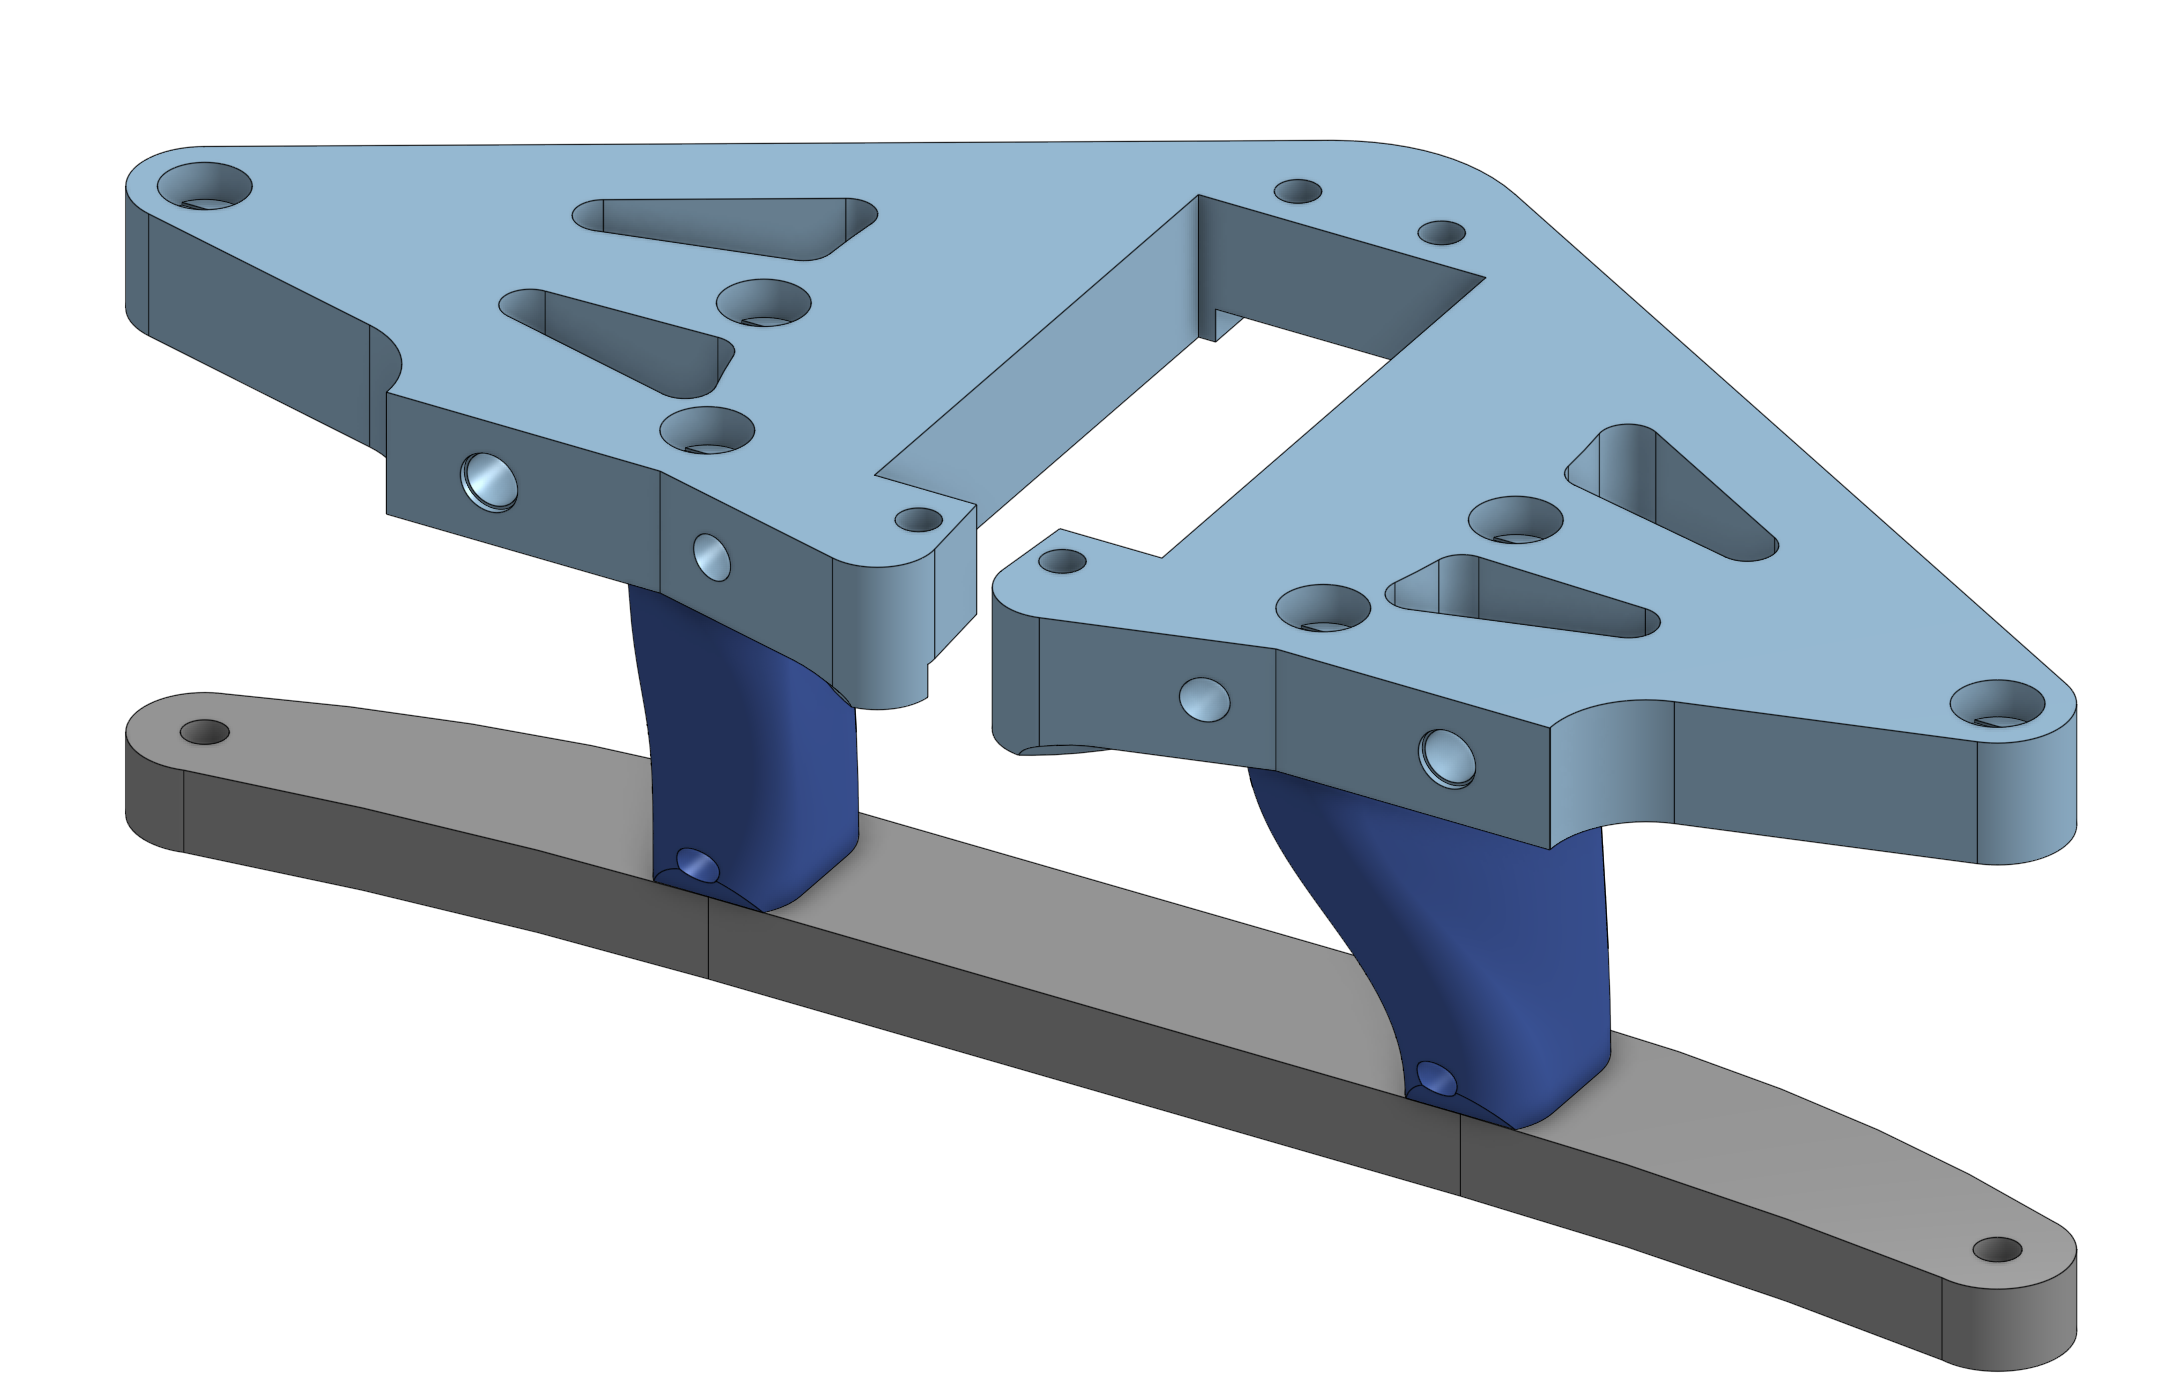
\includegraphics[width=.6\textwidth]{img/steering_col_parts.png}
    \caption{The Steering Column.}
    \label{fig:C_SC} 
\end{figure}

The top brace is the largest part in the steering column. It mounts the servo and the camera. The servo mounts via 4 M$3 \times 20$ screws and has a mounting pattern of $10.5 \times 48$mm. The top brace has an hole at each extreme so that it can interface with the steering knuckle. It does so by using M$3 \times 8$ screws. The holes are space $131$mm apart. The top brace has 4 additional counter bore holes that connect it with the 2 side braces. On the rear face of the mount, there are two locating holes for the carbon fiber rods that are spread apart by $36$mm. There also exists a flat face with space for 2 $M3 \times 6$ heat set inserts so that the part can interface with the rest of the body and is constrained.

\begin{figure}[H]
    \centering
    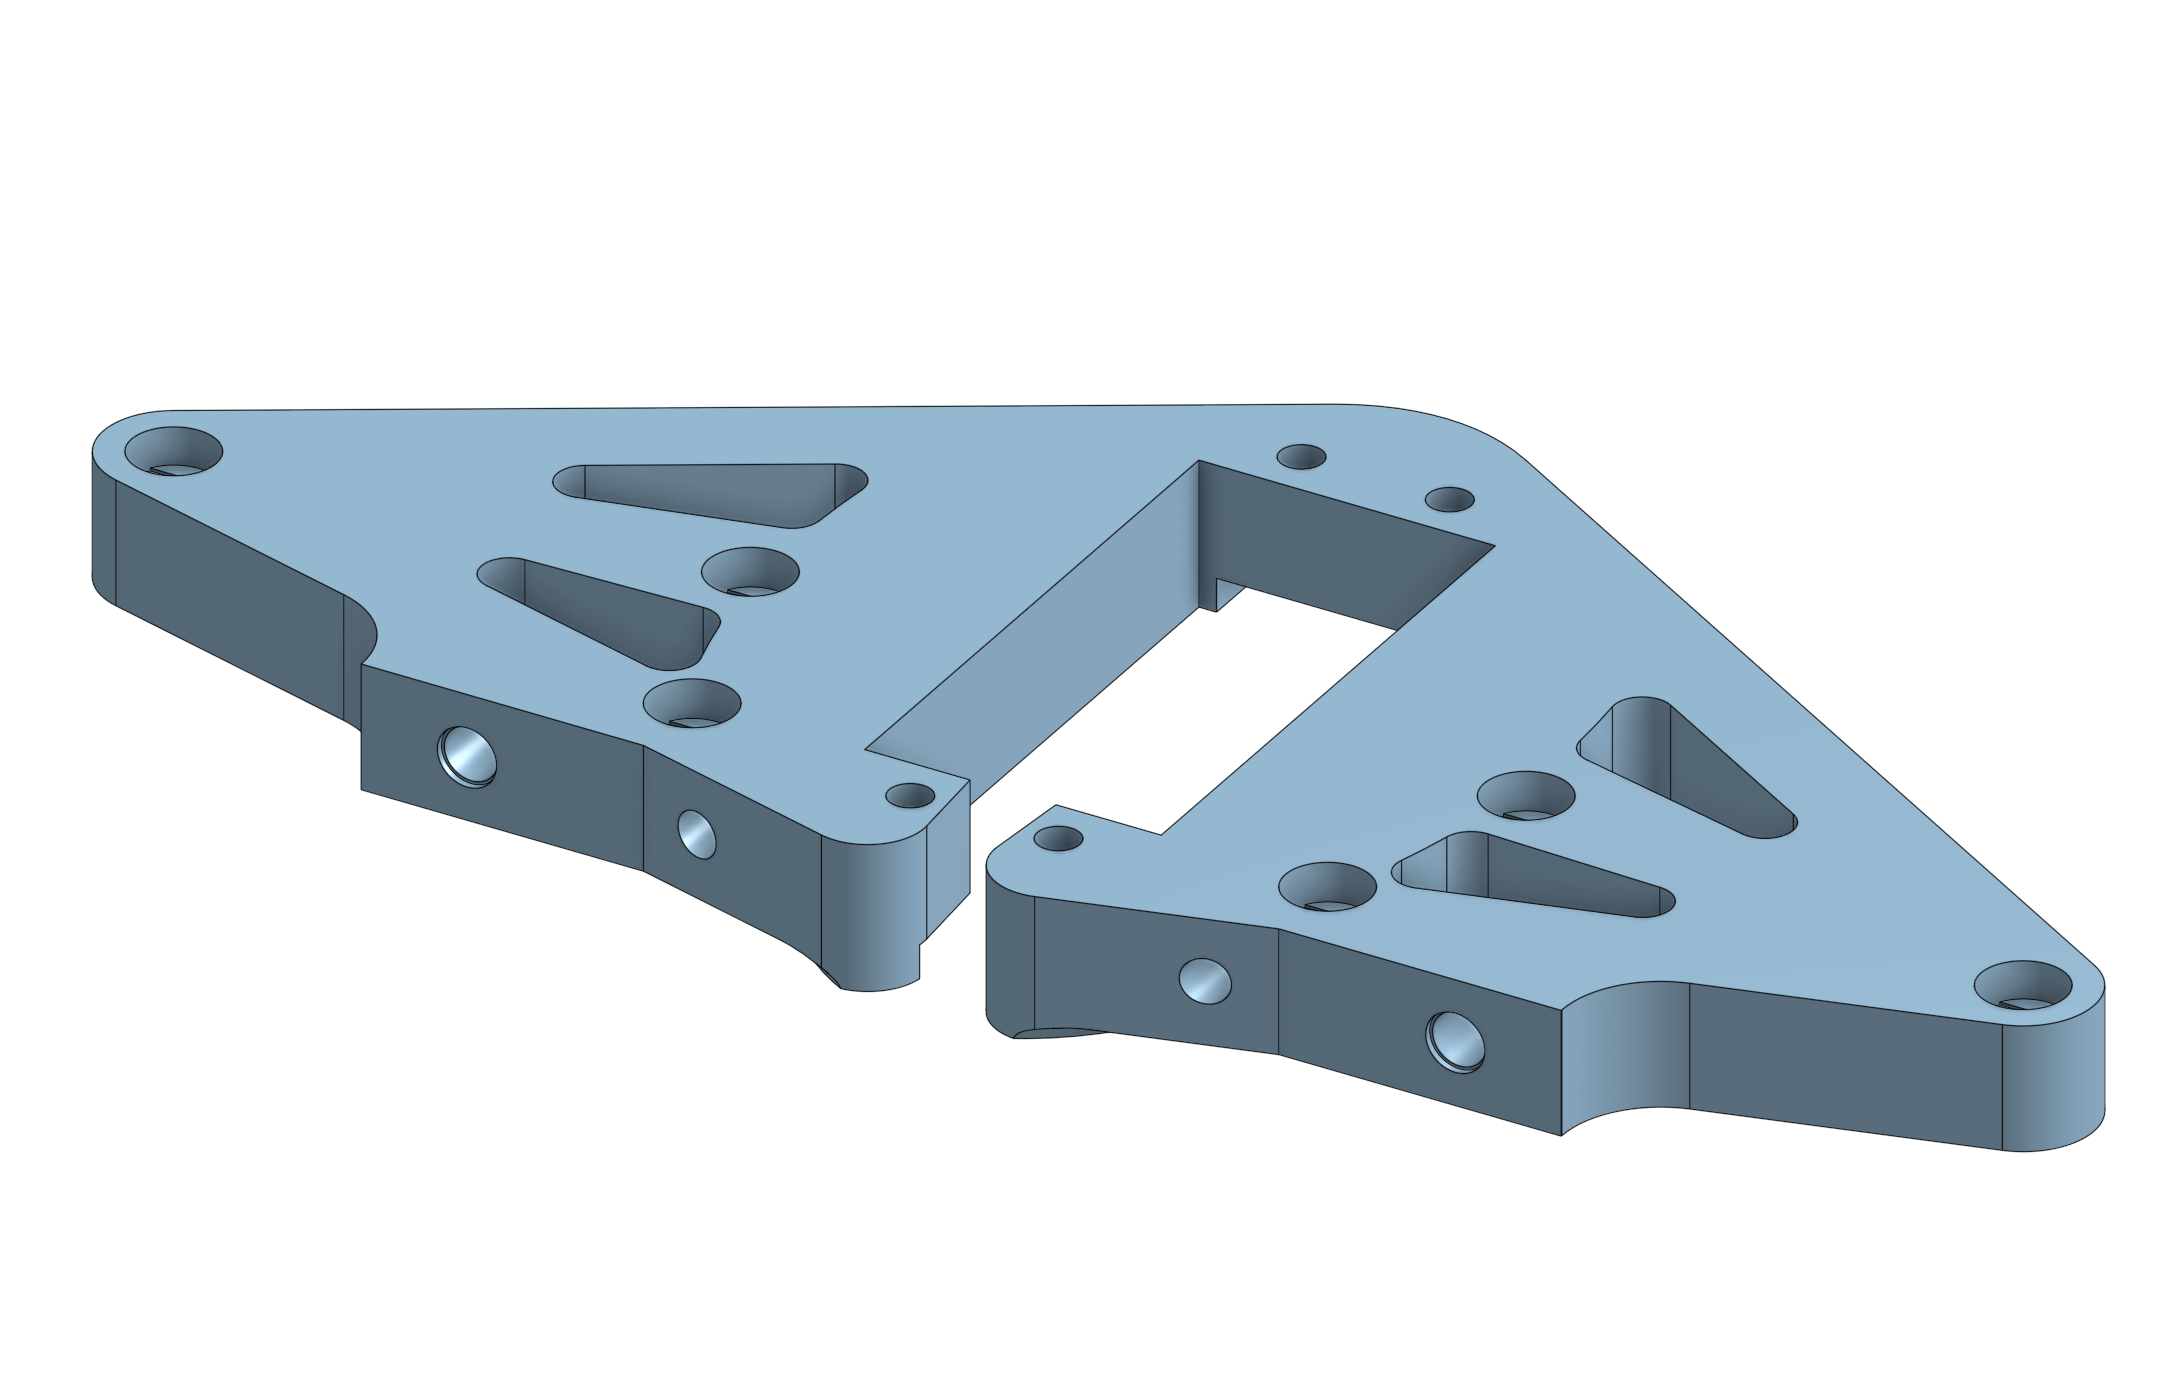
\includegraphics[width=.4\textwidth]{img/top_brace.png}
    \caption{The Top Brace.}
    \label{fig:C_SC_TB} 
\end{figure}

The part is printed with the top face (See Figure \ref{fig:C_SC_TB}) facing down, at a layer height of $0.2$mm, has $3$ perimeters and a $25\%$ infill. The part nominally includes features to aid with counter bore bridging but PreFlight can also be used to aid with this. \\

The bottom brace is the simplest part. It is a slightly curved piece that spans the breadth of the wheelbase. It has $4$ countersunk holes, $2$ to interface with the steering knuckles, and $2$ to interface with the side braces, using M$3 \times 8$mm countersunk and M$3 \times 10$mm countersunk screws respectively. The part is printed with the bottom face (See Figure \ref{fig:C_SC_BB}) facing up, so that the sunk bores are not printed as overhangs. It is printed at a layer height of $0.2$mm, has $3$ perimeters and a $25\%$ infill.

\begin{figure}[H]
    \centering
    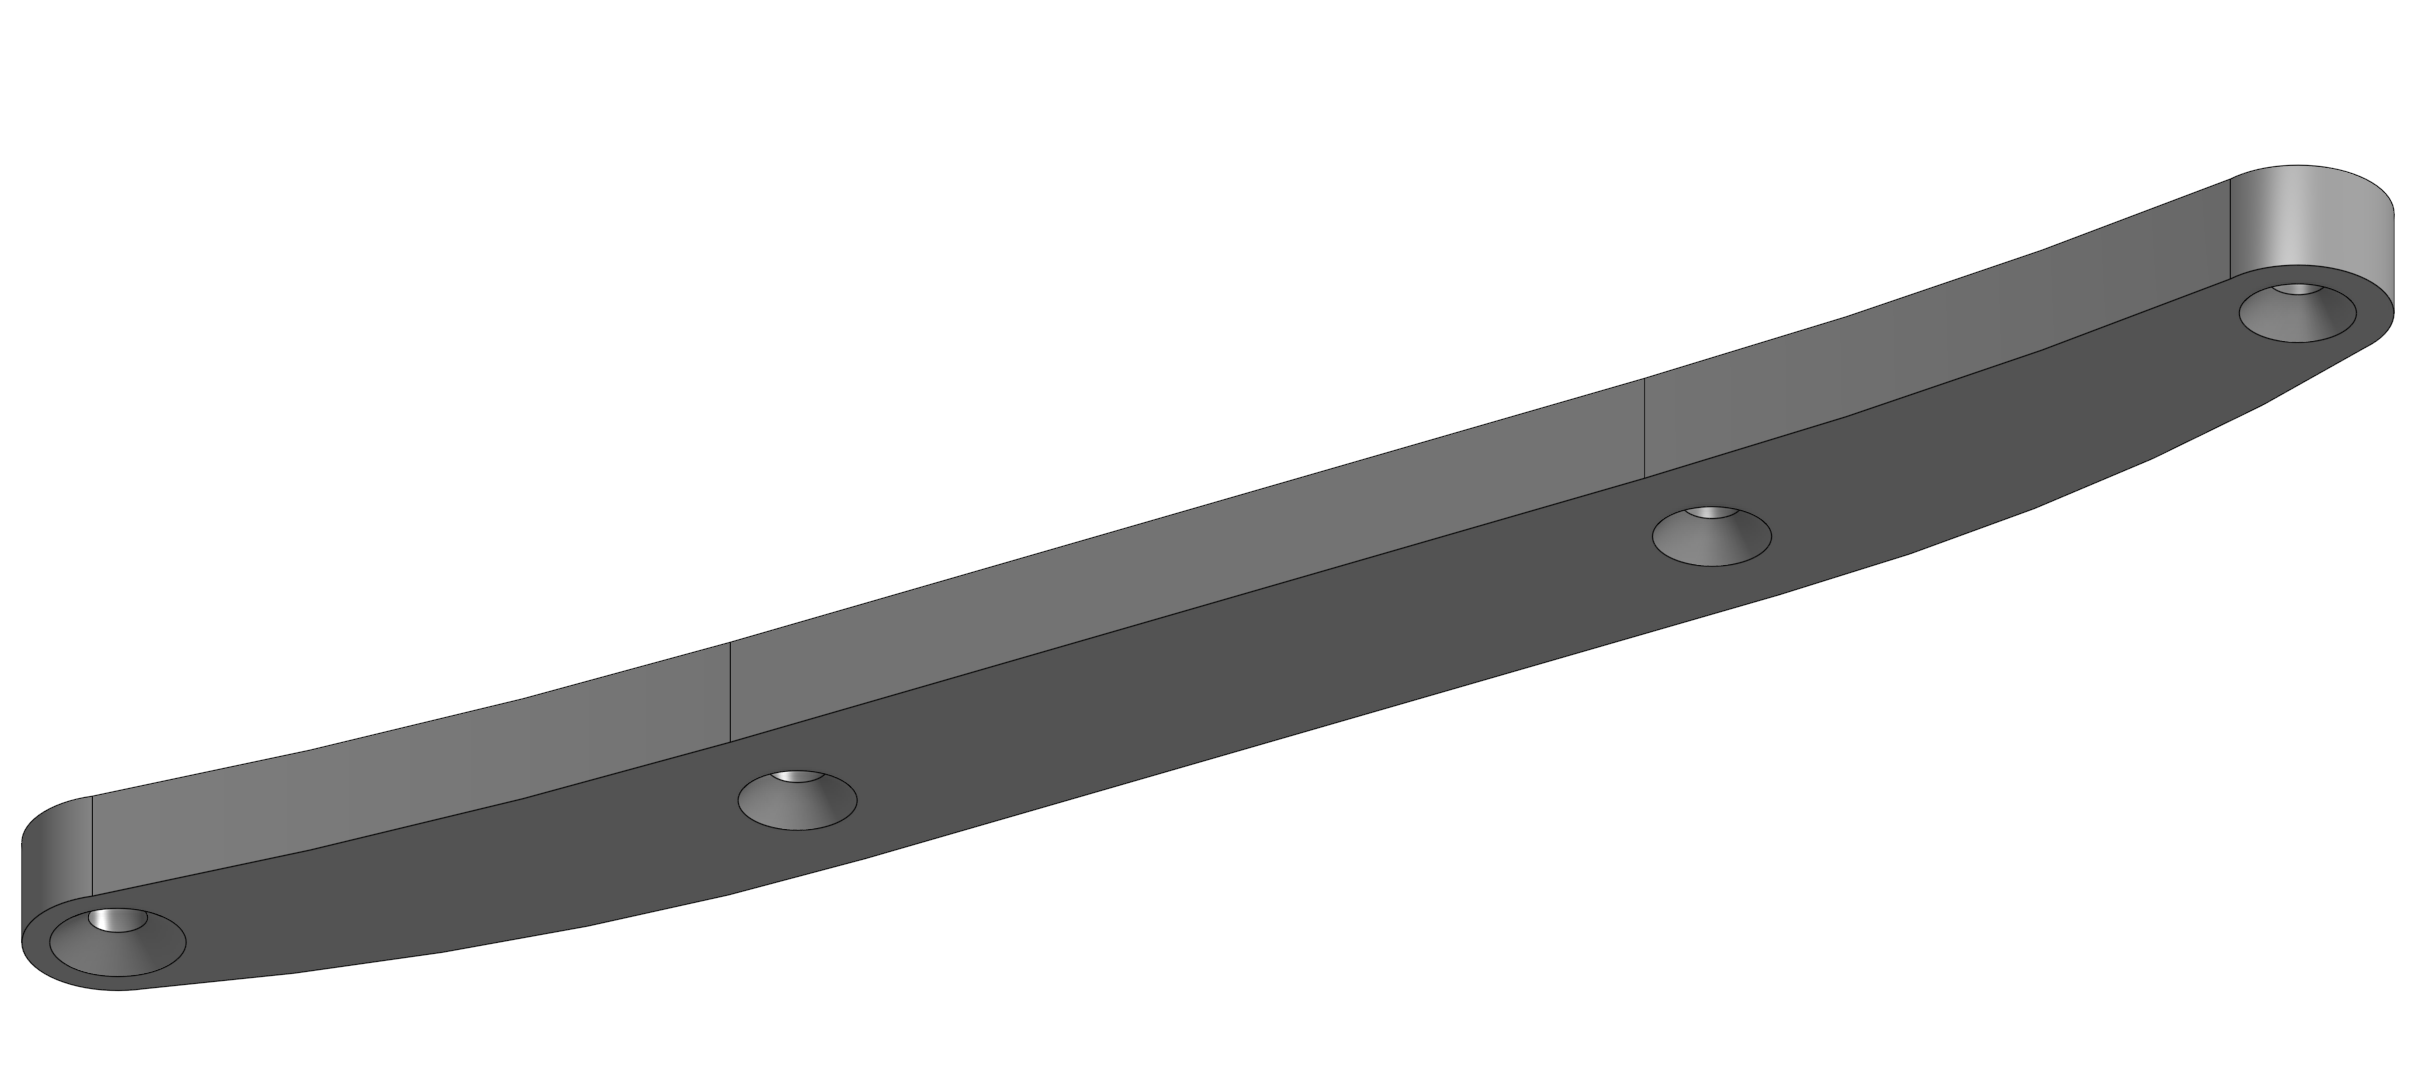
\includegraphics[width=.4\textwidth]{img/bottom_brace.png}
    \caption{The Bottom Brace.}
    \label{fig:C_SC_BB} 
\end{figure}

The side braces are slightly more complex in geometry as they are a product of lofts. The side braces have spaces for $2$ M$3 \times 6$mm brass heat set inserts on the top, and $1$ M$3 \times 6$mm brass heat set inset on the bottom to interface with the top and bottom braces receptively. The side brace also has a feature to interface with the bottom set of $\diameter 3$mm Carbon Fiber Rods. The part is designed for the left and is mirrored to fit for the right side. The part is printed with the top surface facing down, at a layer height of $0.2$mm, has $3$ perimeters and a $25\%$ infill.

\begin{figure}[H]
    \centering
    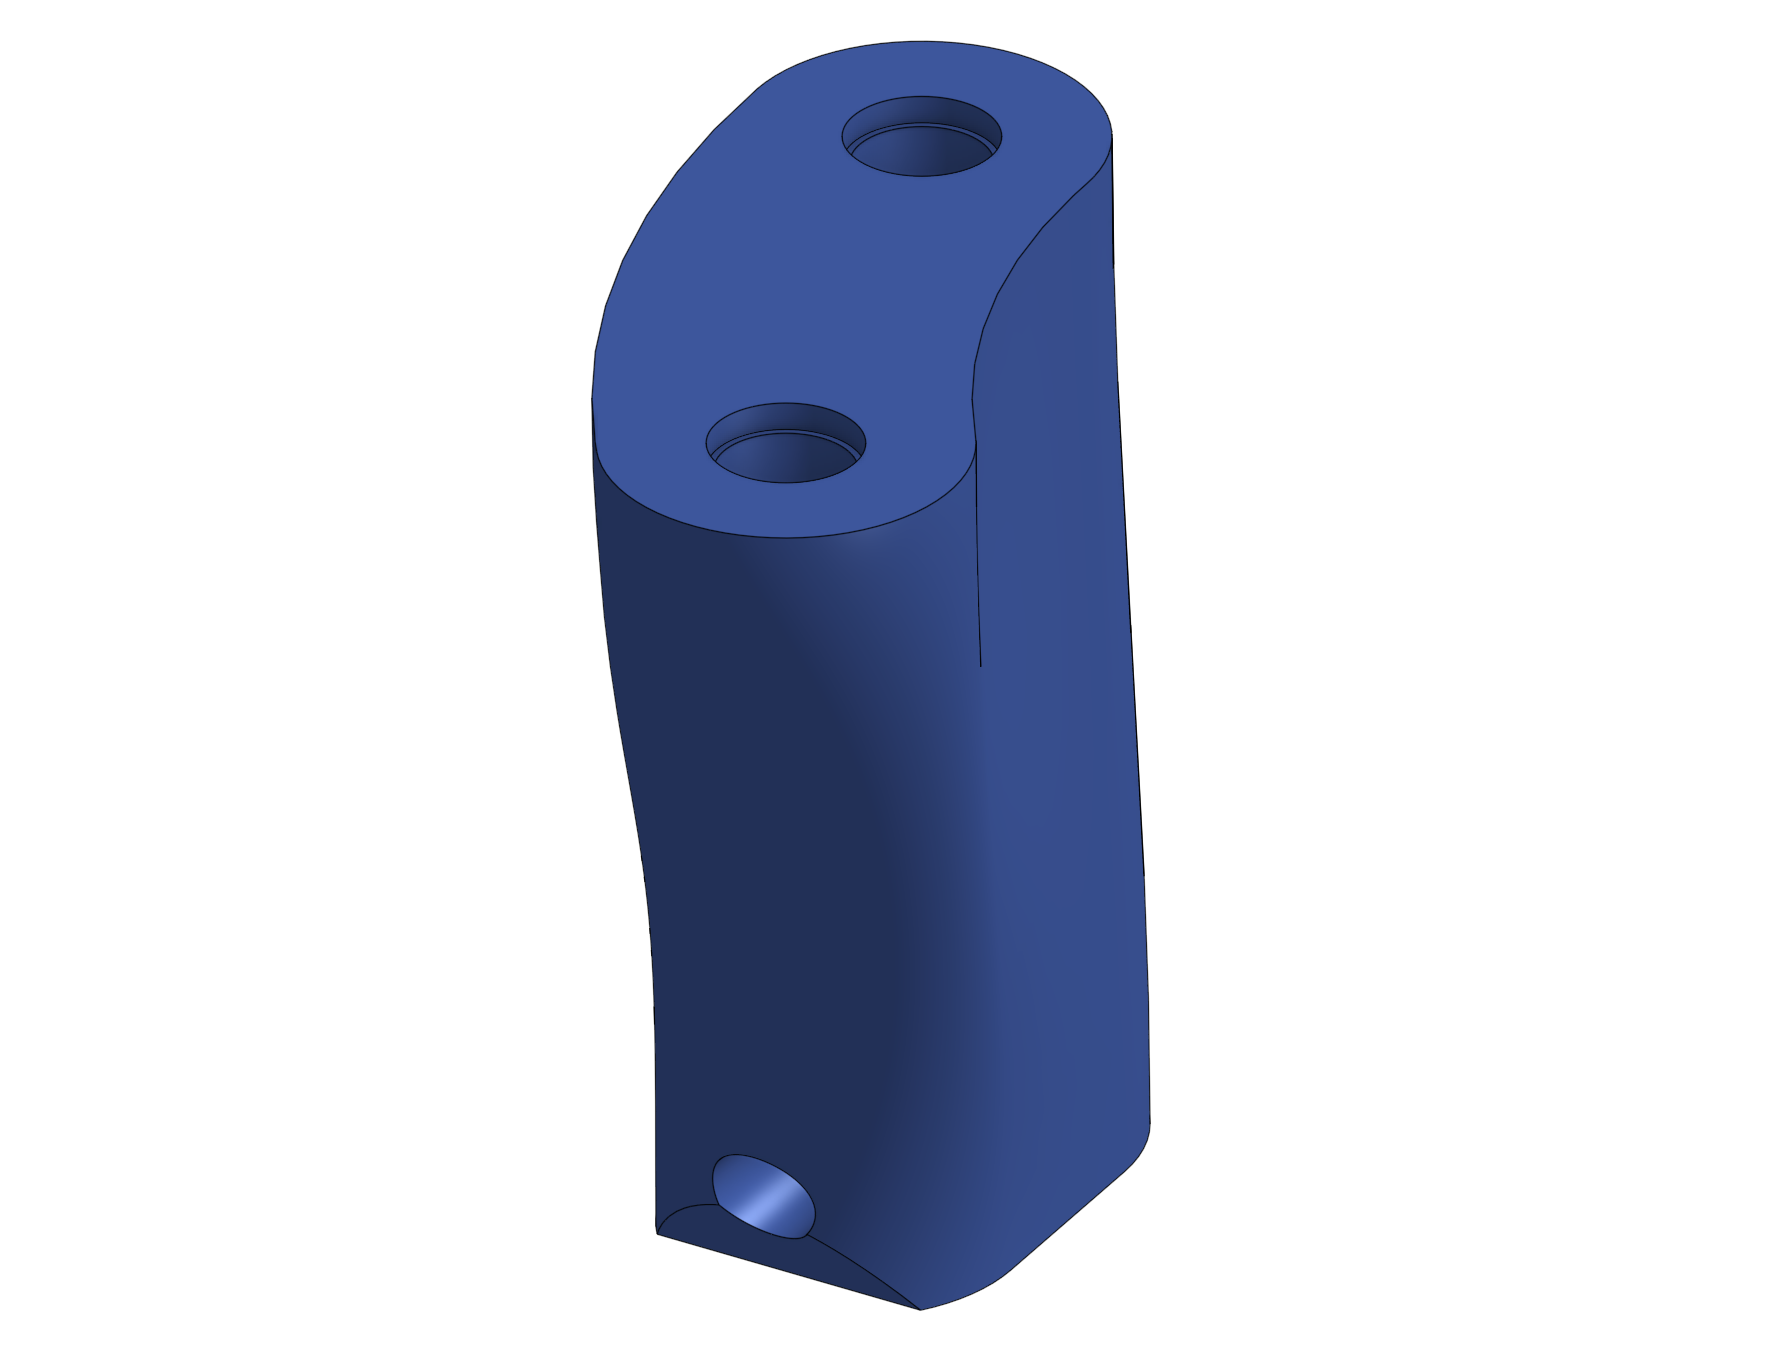
\includegraphics[width=.4\textwidth]{img/side_brace.png}
    \caption{The Side Brace.}
    \label{fig:C_SC_SB} 
\end{figure}

They all combine to form the steering column.

\subsubsection*{Servo Horn}

The servo horn is the part that clamps on the the shaft of thew servo and interfaces with the steering linkage rods. It is a fairly simple part. It houses a $\diameter 6$mm  hole at one end and the space for a M$3 \times 6$ spacer (See Figure \ref{fig:C_SH}, grey) that is press fit into it. The distance between the two is $30$mm. The height of the part is also $6$mm. The part is printed at a layer height of $0.2$mm, has $3$ perimeters and a $25\%$ infill. To maximize the frictional force, the inside surface of the hole is printed with Fuzzy Skin, with a thickness of $0.1$mm and $0.2$mm.

\begin{figure}[H]
    \centering
    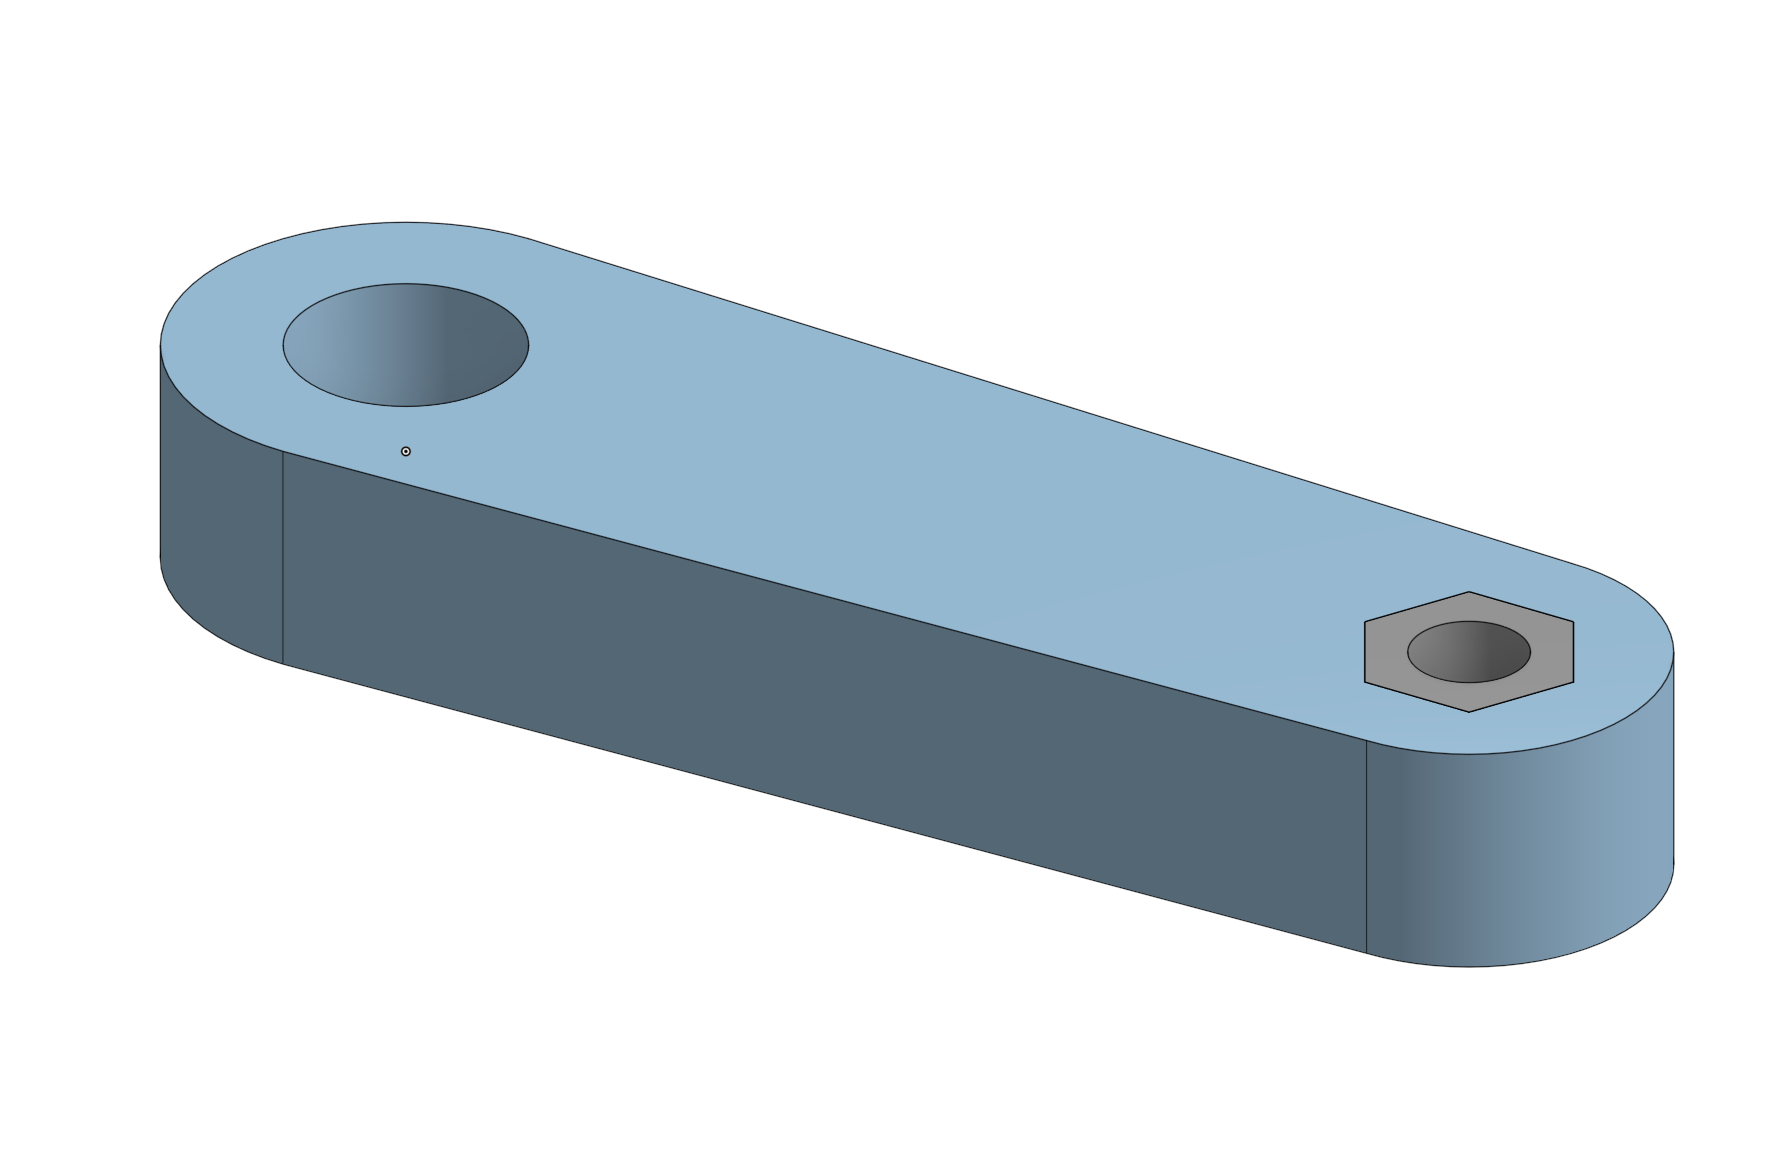
\includegraphics[width=.6\textwidth]{img/servo_horn.png}
    \caption{The Servo Horn.}
    \label{fig:C_SH} 
\end{figure}

\subsubsection*{Steering Links}

The steering links, along with a $\diameter 3$mm Carbon Fiber rod make up the steering rod. The links have $2$ parts (See Figure \ref{fig:C_SL}), one that connects to the servo, the servo link (Figure \ref{fig:C_SL_Servo}) and the other other that connects to the knuckle (Figure \ref{fig:C_SL_Wheel}), the wheel link. The servo link has a height of $7.1$mm with a $\diameter 3$mm hole running through the center for a M$3 \times 10$mm screw. It also has a space for the carbon fiber rod perpendicular to the screw. The wheel link is similar with a height of $5$mm and a hole for a M$2 \times 20$mm screw that connects it to the steering knuckles. The two links rely on the screw as a "pin" to rotate freely. A bearing is not used for this revolute joint as the size is too small to accommodate any and the force are low. The part is printed at a layer height of $0.12$mm, has $3$ perimeters and a solid infill. $2$ sets of these are needed to form the $2$ steering rods. One is mounted at the top and the other at the bottom (Figure \ref{fig:C_SL_Context}).

\begin{figure}[H]
    \centering
    % --- Left Column (Stacked Images) ---
    \begin{subfigure}[b]{0.45\textwidth}
        \centering
        \begin{subfigure}[b]{\textwidth}
            \centering
            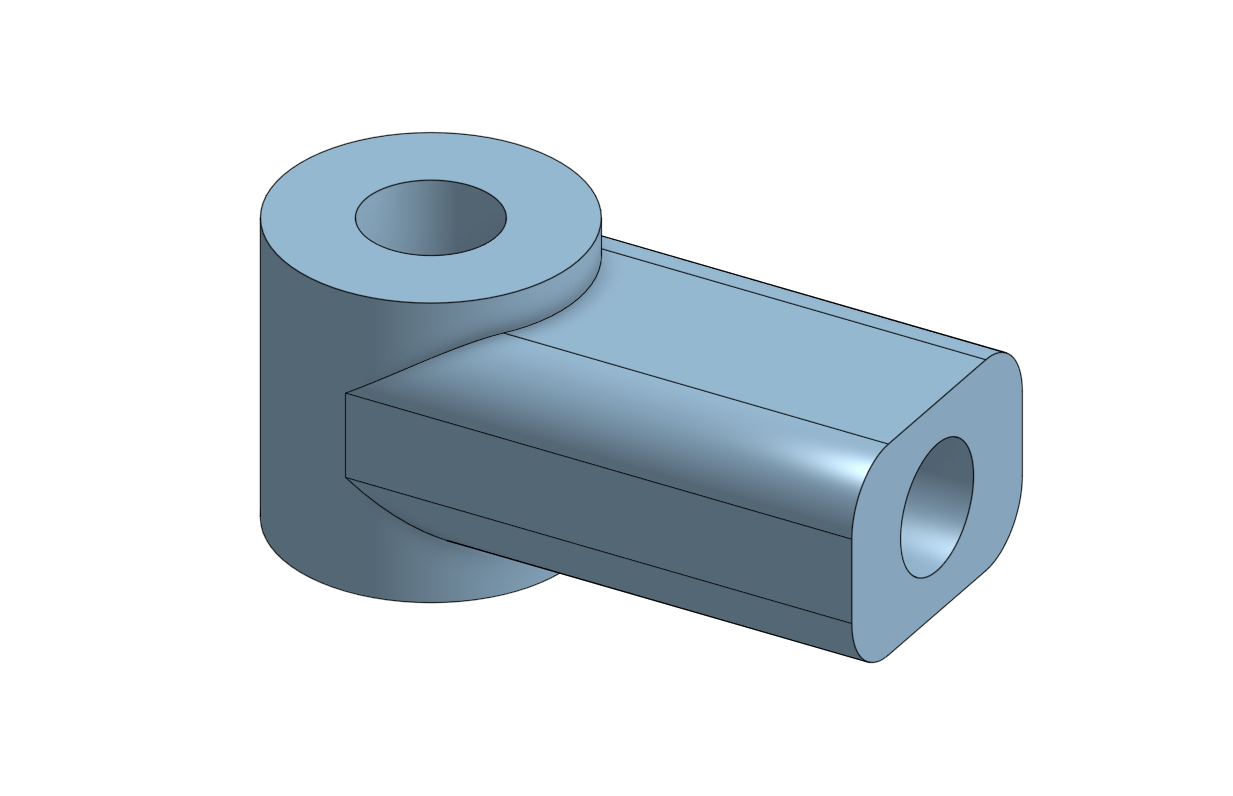
\includegraphics[width=0.85\linewidth]{img/steering_link_1.png}
            \caption{Servo Link}
            \label{fig:C_SL_Servo}
        \end{subfigure}
        
        \vspace{1.5em} % Balanced spacing between the two stacked images
        
        \begin{subfigure}[b]{\textwidth}
            \centering
            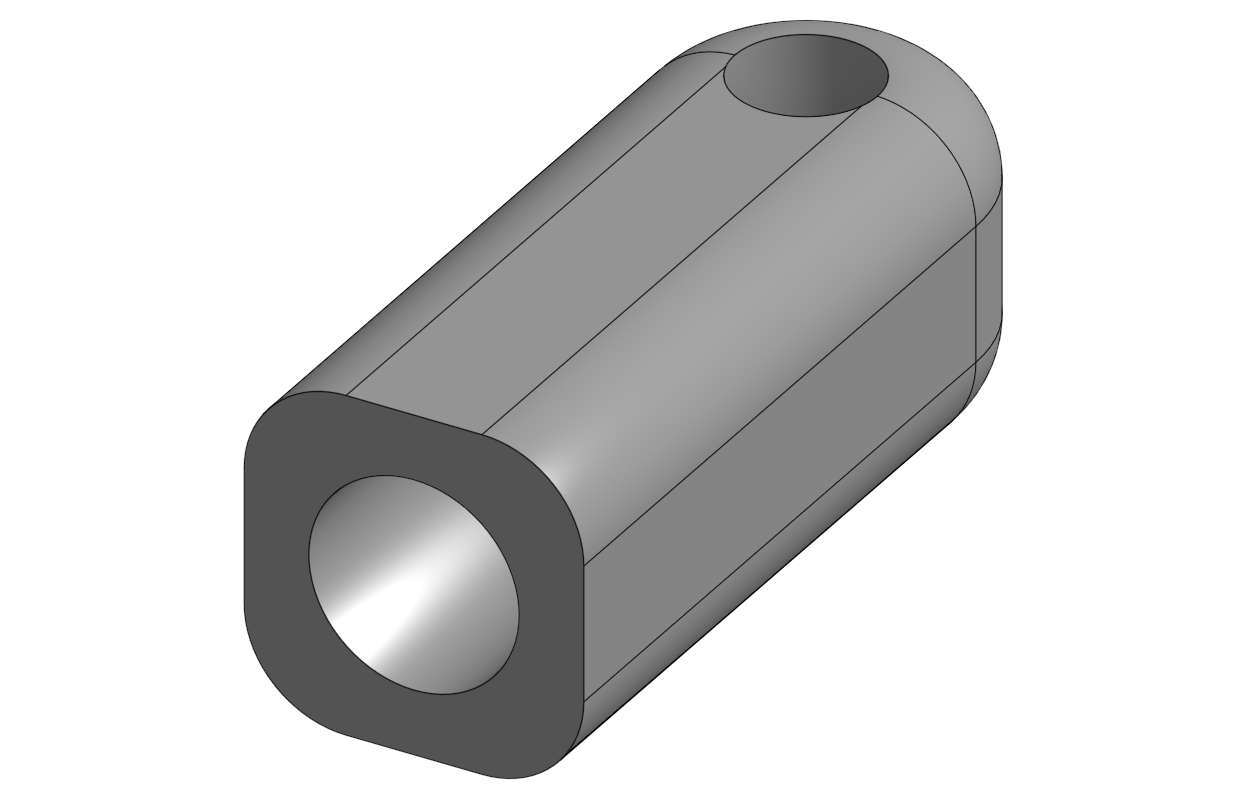
\includegraphics[width=0.85\linewidth]{img/steering_link_2.png}
            \caption{Wheel Link}
            \label{fig:C_SL_Wheel}
        \end{subfigure}
    \end{subfigure}
    \hfill
    % --- Right Column (Vertical Image Aligned to Center) ---
    \begin{subfigure}[b]{0.48\textwidth}
        \centering
        % Using \linewidth ensures it fits cleanly within its column boundary
        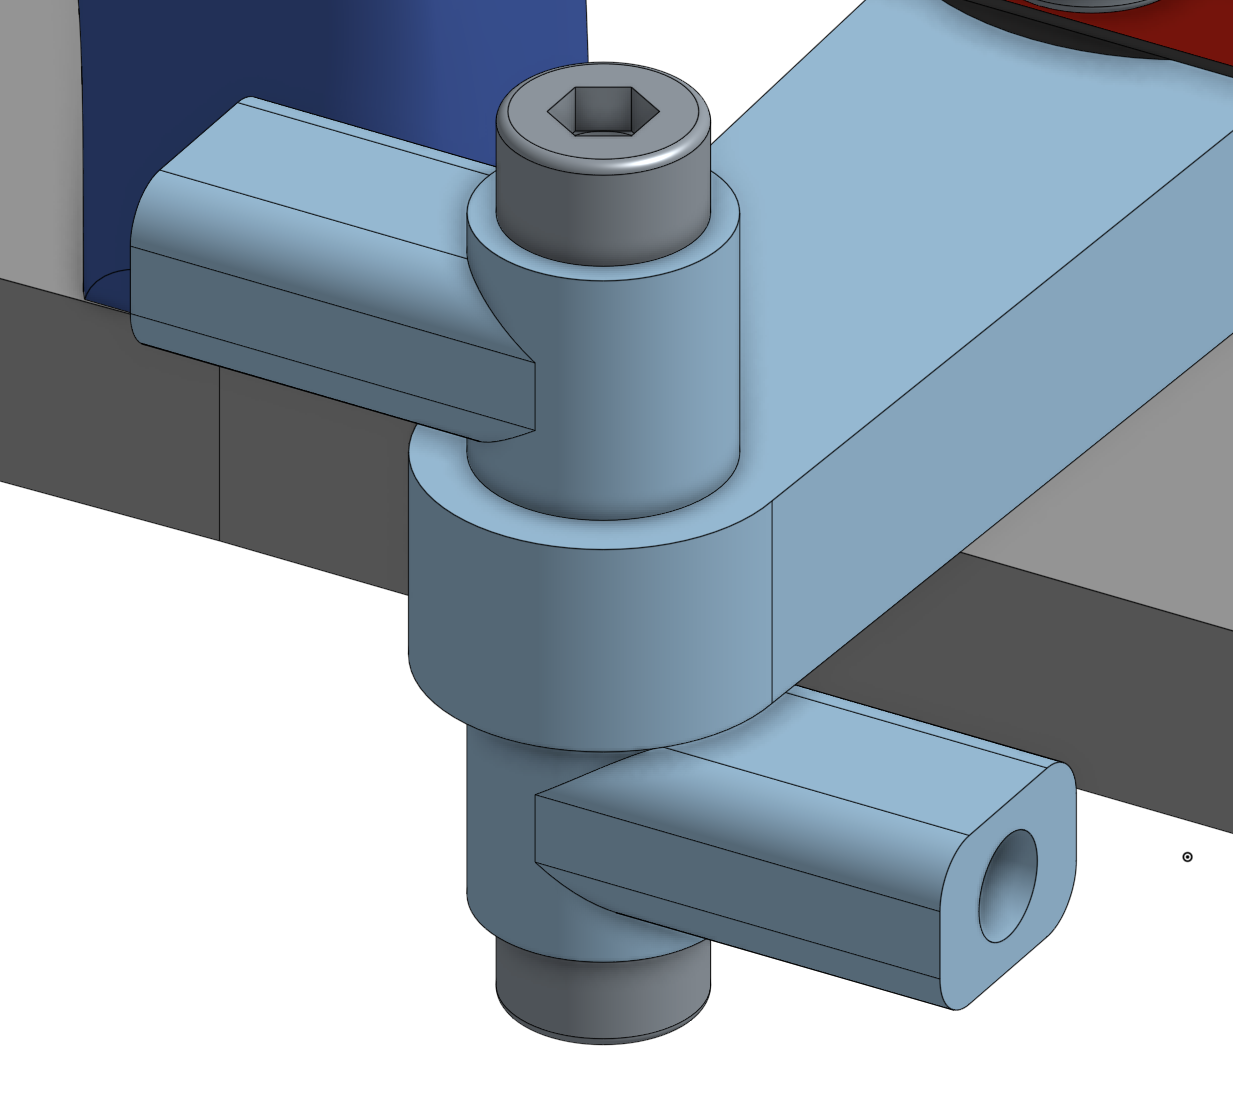
\includegraphics[width=\linewidth, keepaspectratio]{img/steering_link_3.png}
        \caption{Installation Context}
        \label{fig:C_SL_Context}
    \end{subfigure}

    \caption{The Steering Links}
    \label{fig:C_SL}
\end{figure}

\subsubsection*{TPU Spacer/Shim}

A Outer $\diameter 16$mm and inner $\diameter 12.80$mm spacer, with a height of $6$mm is needed. This sits between the bearing and the wheel and provides pre-load to the whole stack up. This is used as the roller thrust bearing is only constrained in one direction by the end cap. The other end is hence constrained by the TPU spacer and the pre-load it provides. The pre-load also ensures there is as little play between the axle and the bearing as possible. Figure \ref{fig:C_TPUS} (red) shows the placement of the spacer in section view. Since it is made out of a flexible material with a shore hardness of $95$A, the height of the spacer determines the pre-load force. The part is printed at a layer height of $0.2$mm, has $3$ perimeters and a solid infill. It is utilized on both sides.

\begin{figure}[H]
    \centering
    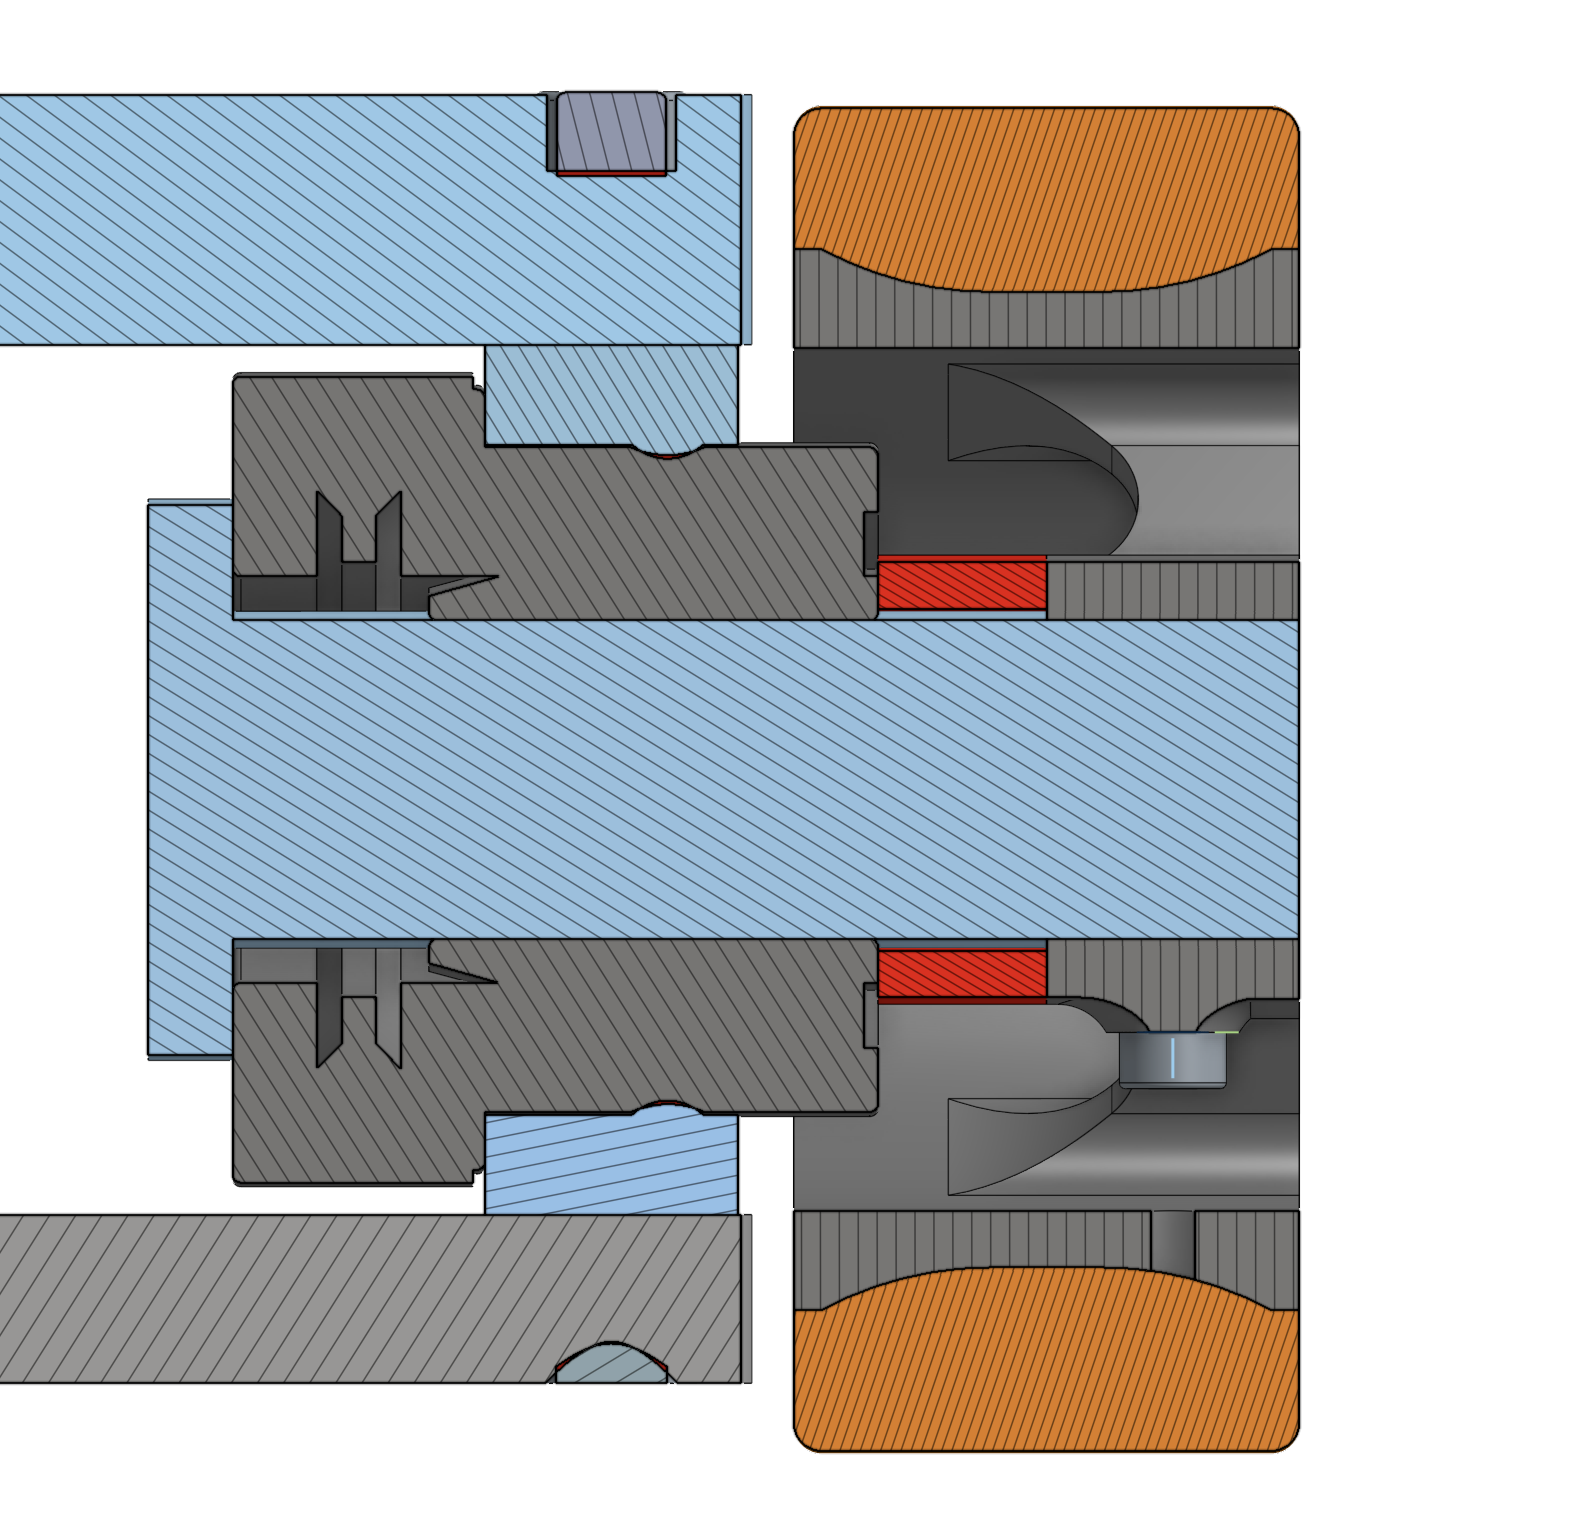
\includegraphics[width=.6\textwidth]{img/tpu_spacer.png}
    \caption{The TPU Spacer.}
    \label{fig:C_TPUS} 
\end{figure}

This concludes the assembly of the front axle. The length of the $\diameter 3$mm carbon fiber rod used in the steering links is $\approx 48$mm. It is glued to the steering links. 

\subsection{The Differential}

\begin{figure}[H]
    \centering
    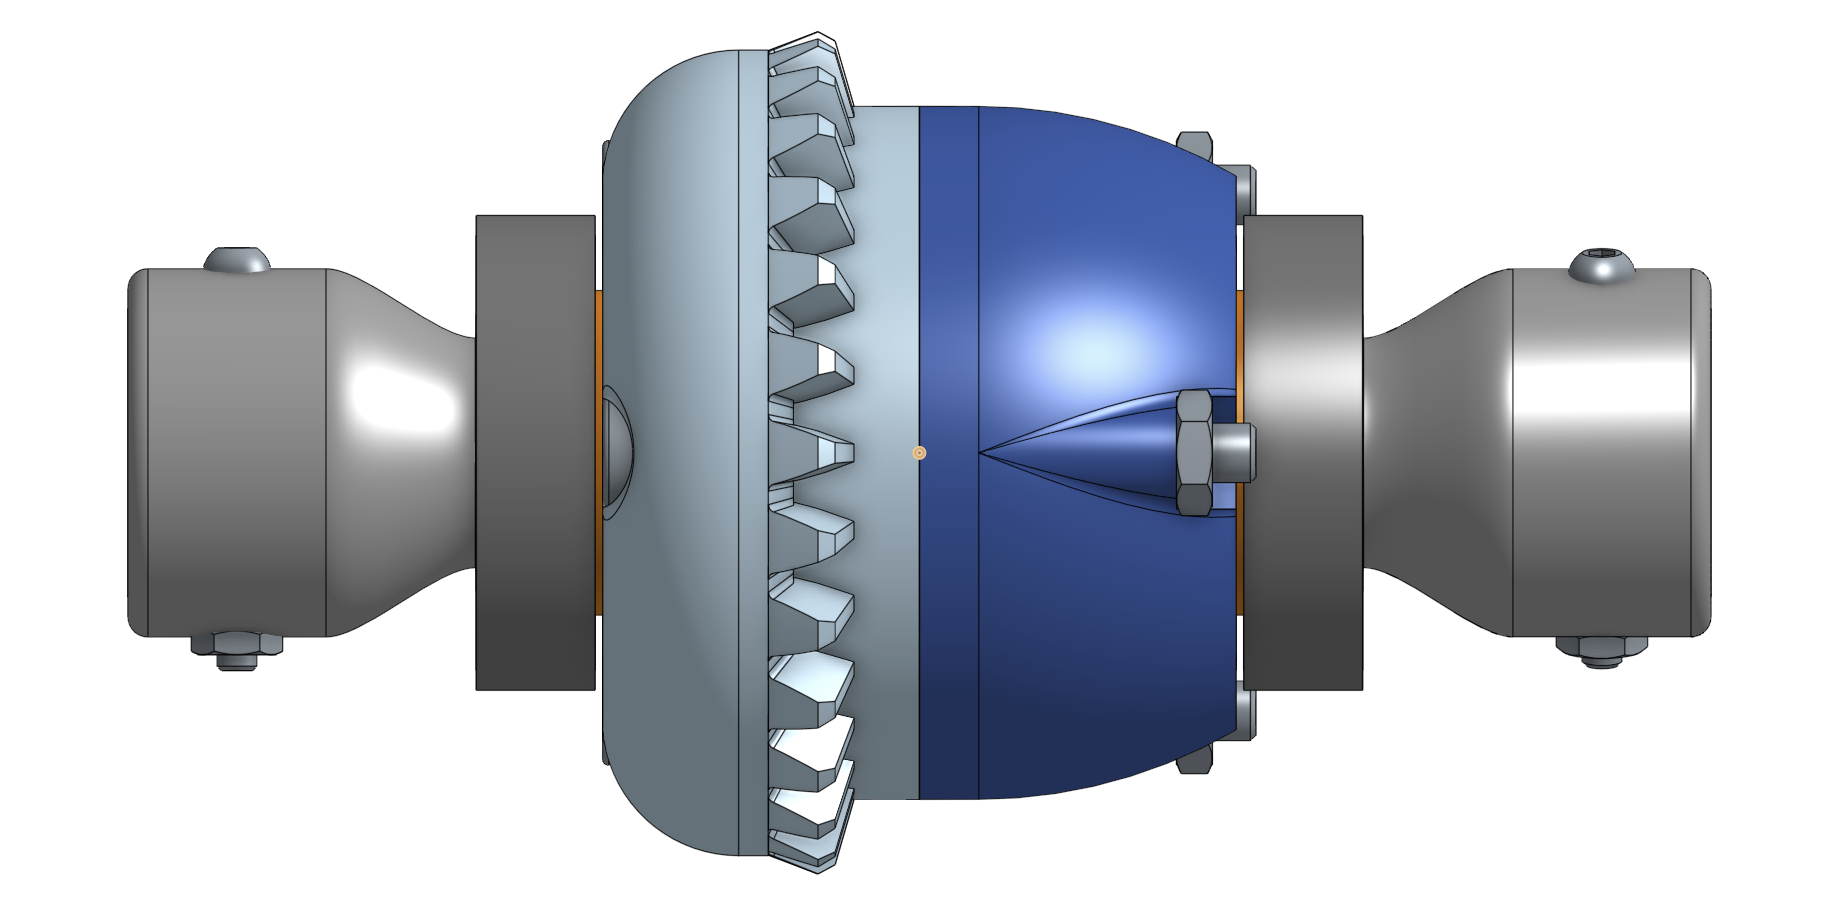
\includegraphics[width=.9\textwidth]{img/diff_gearbox.png}
    \caption{The Differential Gearbox.}
    \label{fig:C_DG_Assem} 
\end{figure}

As mentioned earlier, a differential gear box is used. The center of the gearbox is formed by the "spider" gears and the carrier along with the main gearbox. In a differential gearbox, the housing containing the spider and main gears also rotates and is mounted to a stationary mount. The housing contains the main gear reduction for the differential. The spider gears assist with the difference in speeds of the two main gears (and hence wheels). All of the parts of the gearbox are 3D printed. The net reduction produced is $8:28 = 2:7$.

\subsubsection*{The Gears}

The differential consists of $3$ spider gears and $2$ main gears All the gears present are bevel gears created using the OnShape bevel gear scripts. \\

The spider gears have $9$ teeth, a module of $1.5$mm, a pressure angle of $20^{\circ}$ and a bevel angle of $30.96^{\circ}$. The spider gears have a $\diameter 3$mm hole through the center to interface with the axle. The top has be flattened to aid with printing. They are set $120^{\circ}$ apart. See Figure \ref{fig:C_DG_SG}. \\

The main gears have $15$ teeth, a module of $1.5$mm, a pressure angle of $20^{\circ}$ and a bevel angle of $59.04^{\circ}$. Notice that the bevel angles of the 2 types add up to $90^{\circ}$. The main gear transfer all the load to the wheels. Hence, using a single screw in the center would cause it to loosen due to the torque caused. Hence, $2$ screws are use that are placed $3$mm apart from the center to connect the gears to the part that interfaces with the rear axles. Behind the gear sits a $\diameter 12$mm $\times 11$mm cylinder that interfaces with the bearings. The top has be flattened to aid with printing. See Figure \ref{fig:C_DG_MG}.

\begin{figure}[H]
    \centering
    % --- Left Column (Stacked Images) ---
    \begin{subfigure}[b]{0.45\textwidth}
        \centering
        \begin{subfigure}[b]{\textwidth}
            \centering
            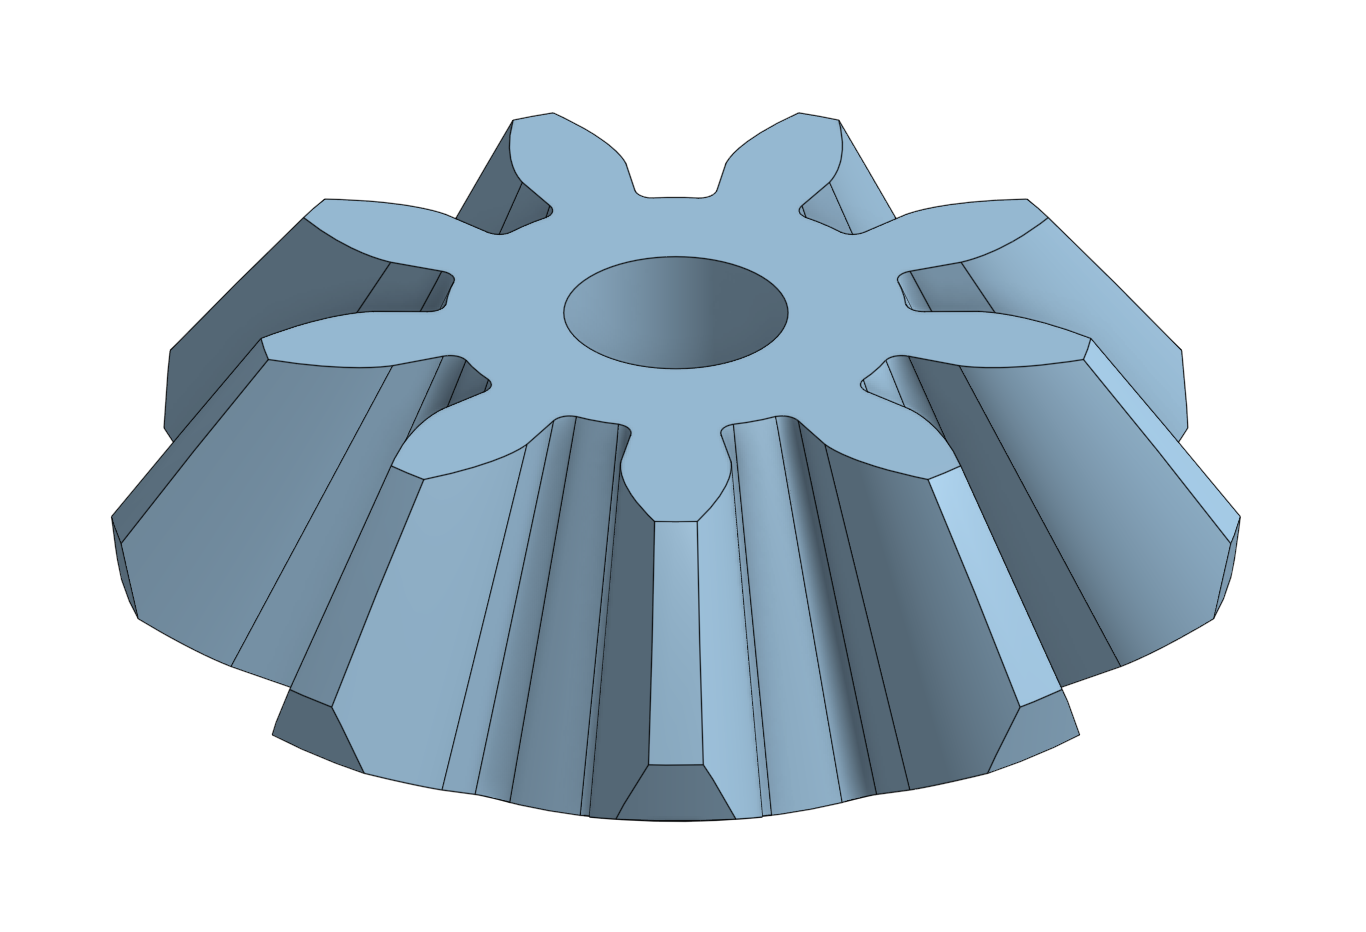
\includegraphics[width=0.85\linewidth]{img/diff_gear_1.png}
            \caption{The Spider Gear}
            \label{fig:C_DG_SG}
        \end{subfigure}
        
        \vspace{1.5em} % Balanced spacing between the two stacked images
        
        \begin{subfigure}[b]{\textwidth}
            \centering
            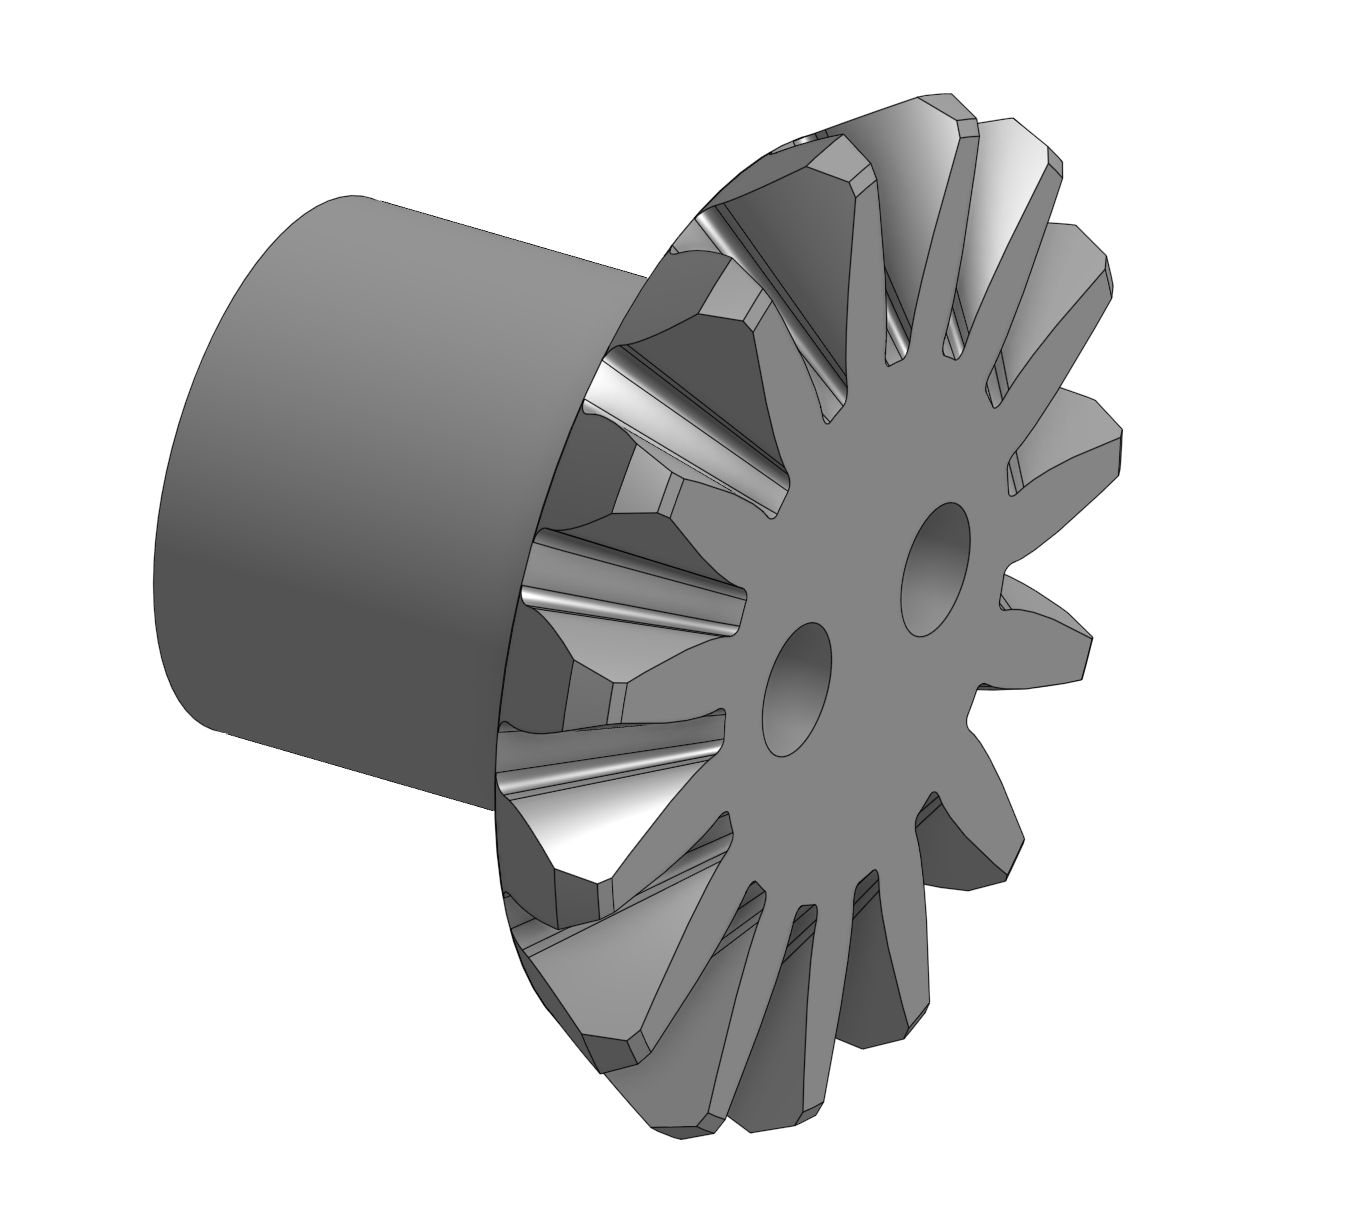
\includegraphics[width=0.85\linewidth]{img/diff_gear_2.png}
            \caption{The Main Gear}
            \label{fig:C_DG_MG}
        \end{subfigure}
    \end{subfigure}
    \hfill
    % --- Right Column (Vertical Image Aligned to Center) ---
    \begin{subfigure}[b]{0.48\textwidth}
        \centering
        % Using \linewidth ensures it fits cleanly within its column boundary
        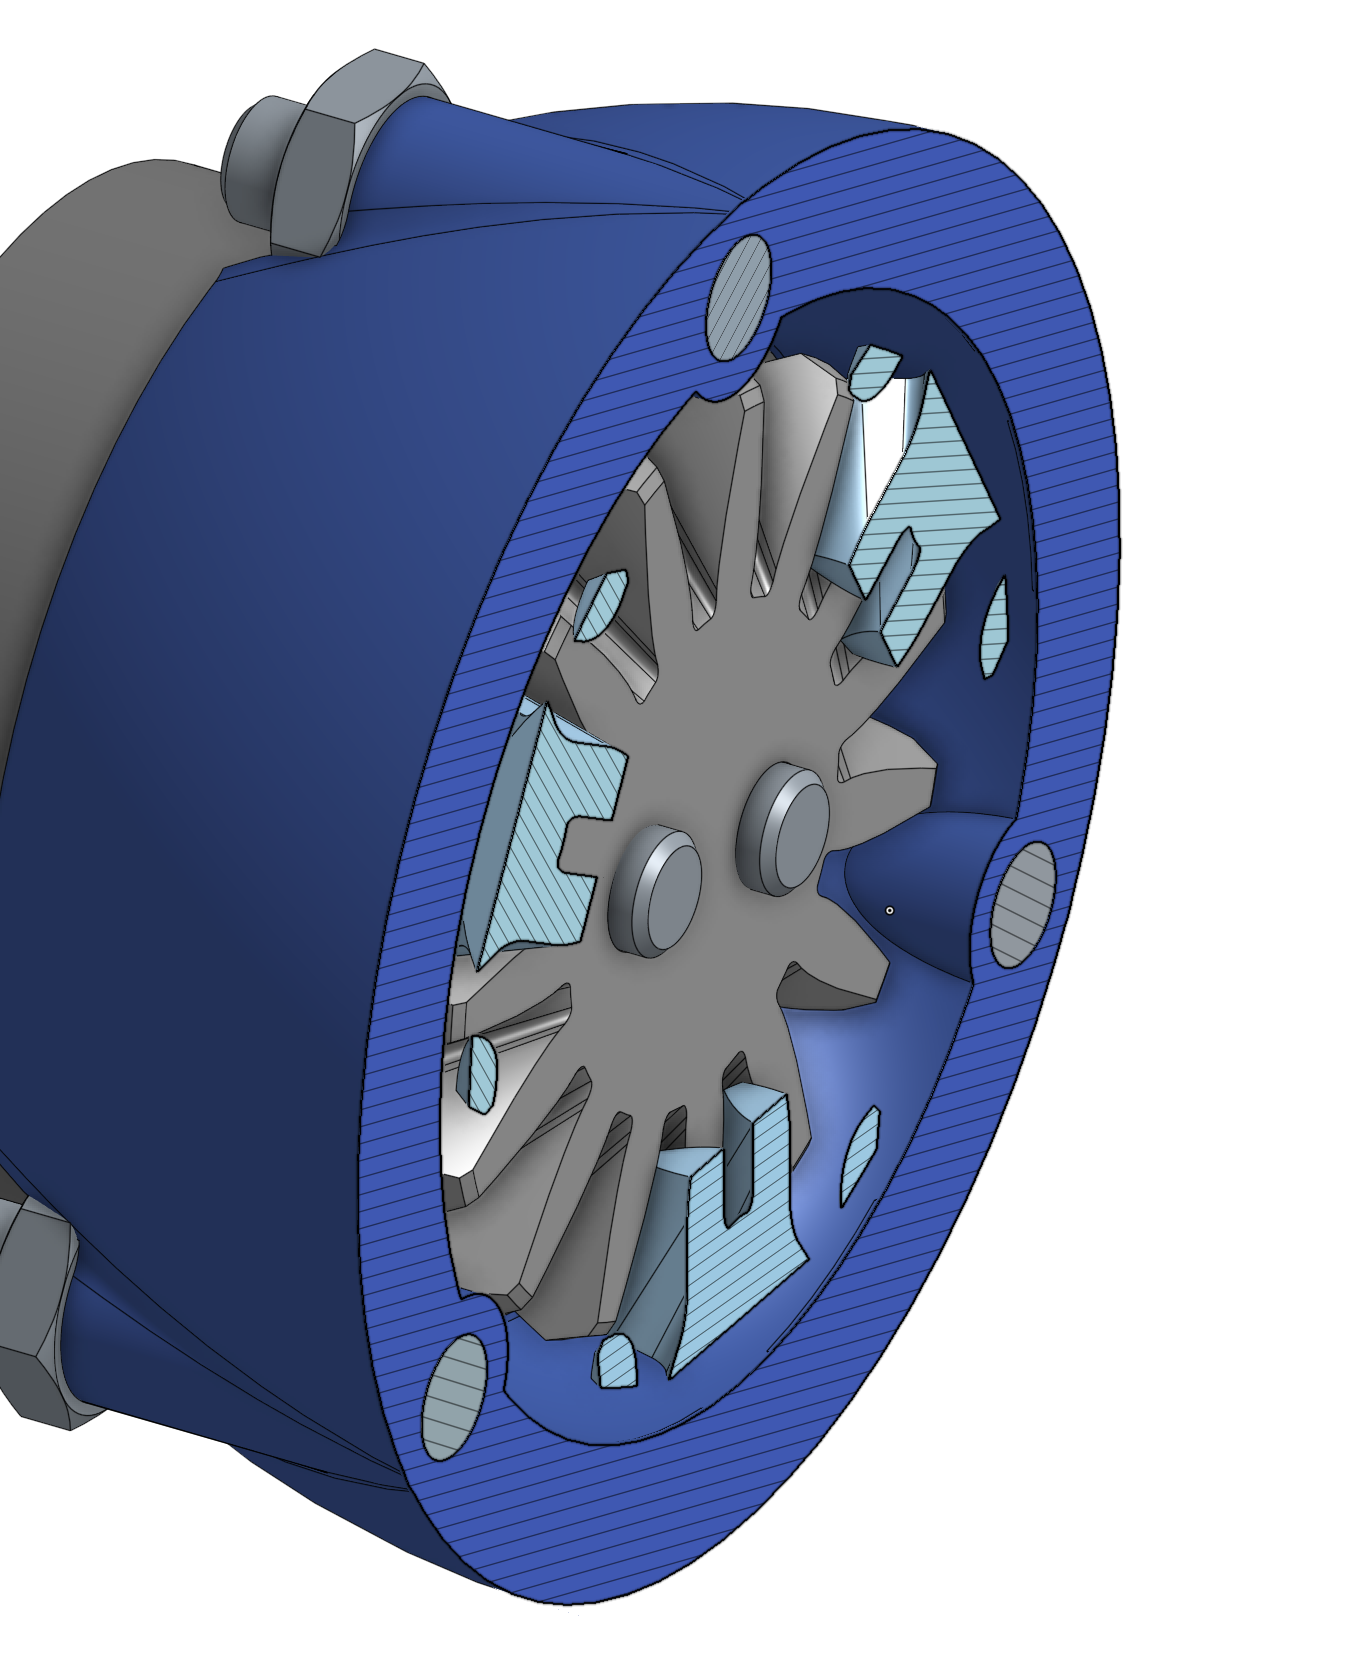
\includegraphics[width=\linewidth, keepaspectratio]{img/diff_gear_3.png}
        \caption{Installation Context}
        \label{fig:C_DG_Context}
    \end{subfigure}
    \caption{The Differential Gears}
    \label{fig:C_DG}
\end{figure}

All 5 of the parts are printed at a layer height of $0.12$mm, has $3$ perimeters and a solid infill. A brim is used to aid with bed adhesion. The spider gears and the main gears are printed with the gear face facing down. This means that the forces of the gears runs along the layer. However, this means that the rotational force of the main gear to the wheels runs across the layer lines, which would mean that the are where the gear ends and the cylinder starts is the weakest area. To counter this, the M$3 \times 20$ button head screws that are used to connect the main gear and the axles run all the way to the end of the gear, meaning they transfer most of the rotational loads and strengthen the part's function across the layer lines. See figure \ref{fig:C_DG_Context}.

\subsubsection*{The Carrier/Spider Center}

The Spider Center is the part that holds all the spider hears in the center and aligns them. In the housing, it is suspended by the M$3 \times 10$mm Button Head screws. See Figure \ref{fig:C_DG_SC}. \\

It's a filleted triangle with 3 $\diameter 3$mm holes on each side. It has a height of $6$mm. It is printed at a layer height of $0.12$mm, has $3$ perimeters and a solid infill. A brim is used to aid with bed adhesion. The part can be printed on either of the larger, flat surfaces.

\begin{figure}[H]
    \centering
    \begin{subfigure}[b]{0.48\textwidth}
        \centering
        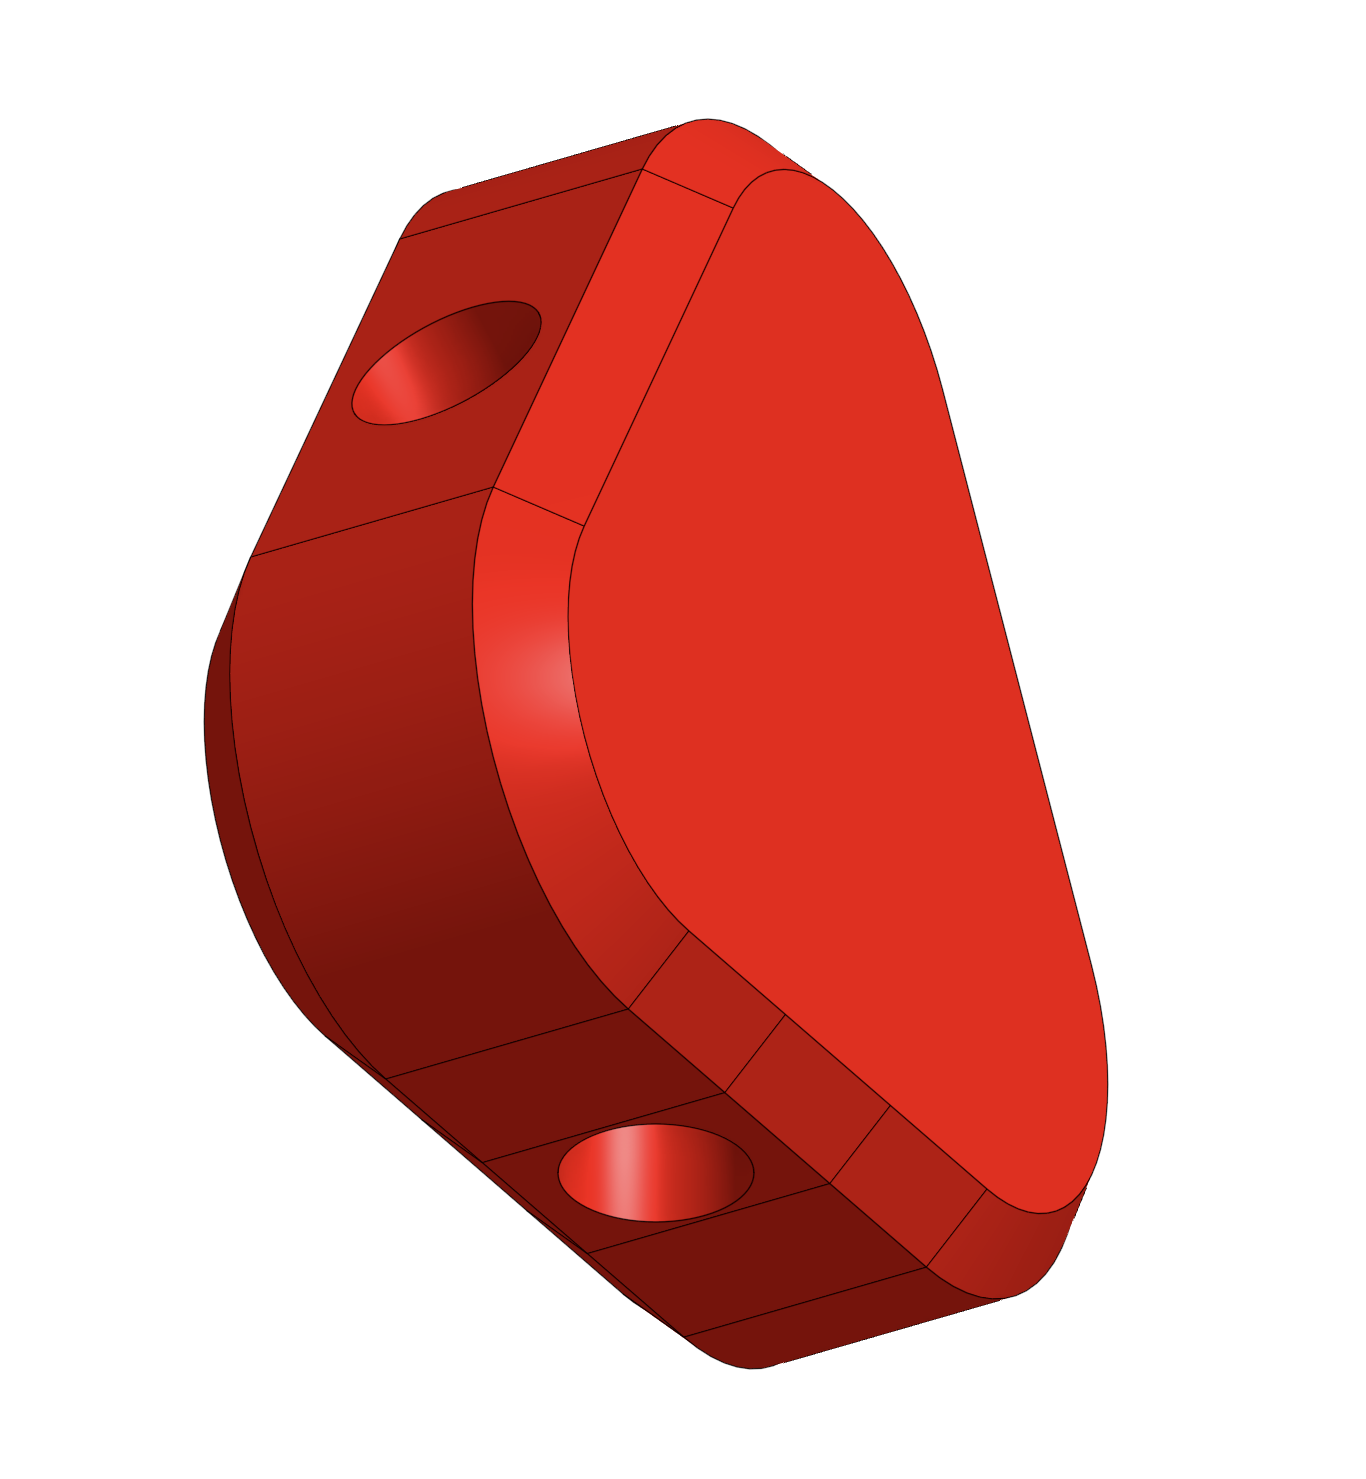
\includegraphics[width=\linewidth, height=0.4\textheight, keepaspectratio]{img/diff_sc_1.png}
        \caption{The Part.}
        \label{fig:diff_sc_1}
    \end{subfigure}
    \hfill
    \begin{subfigure}[b]{0.48\textwidth}
        \centering
        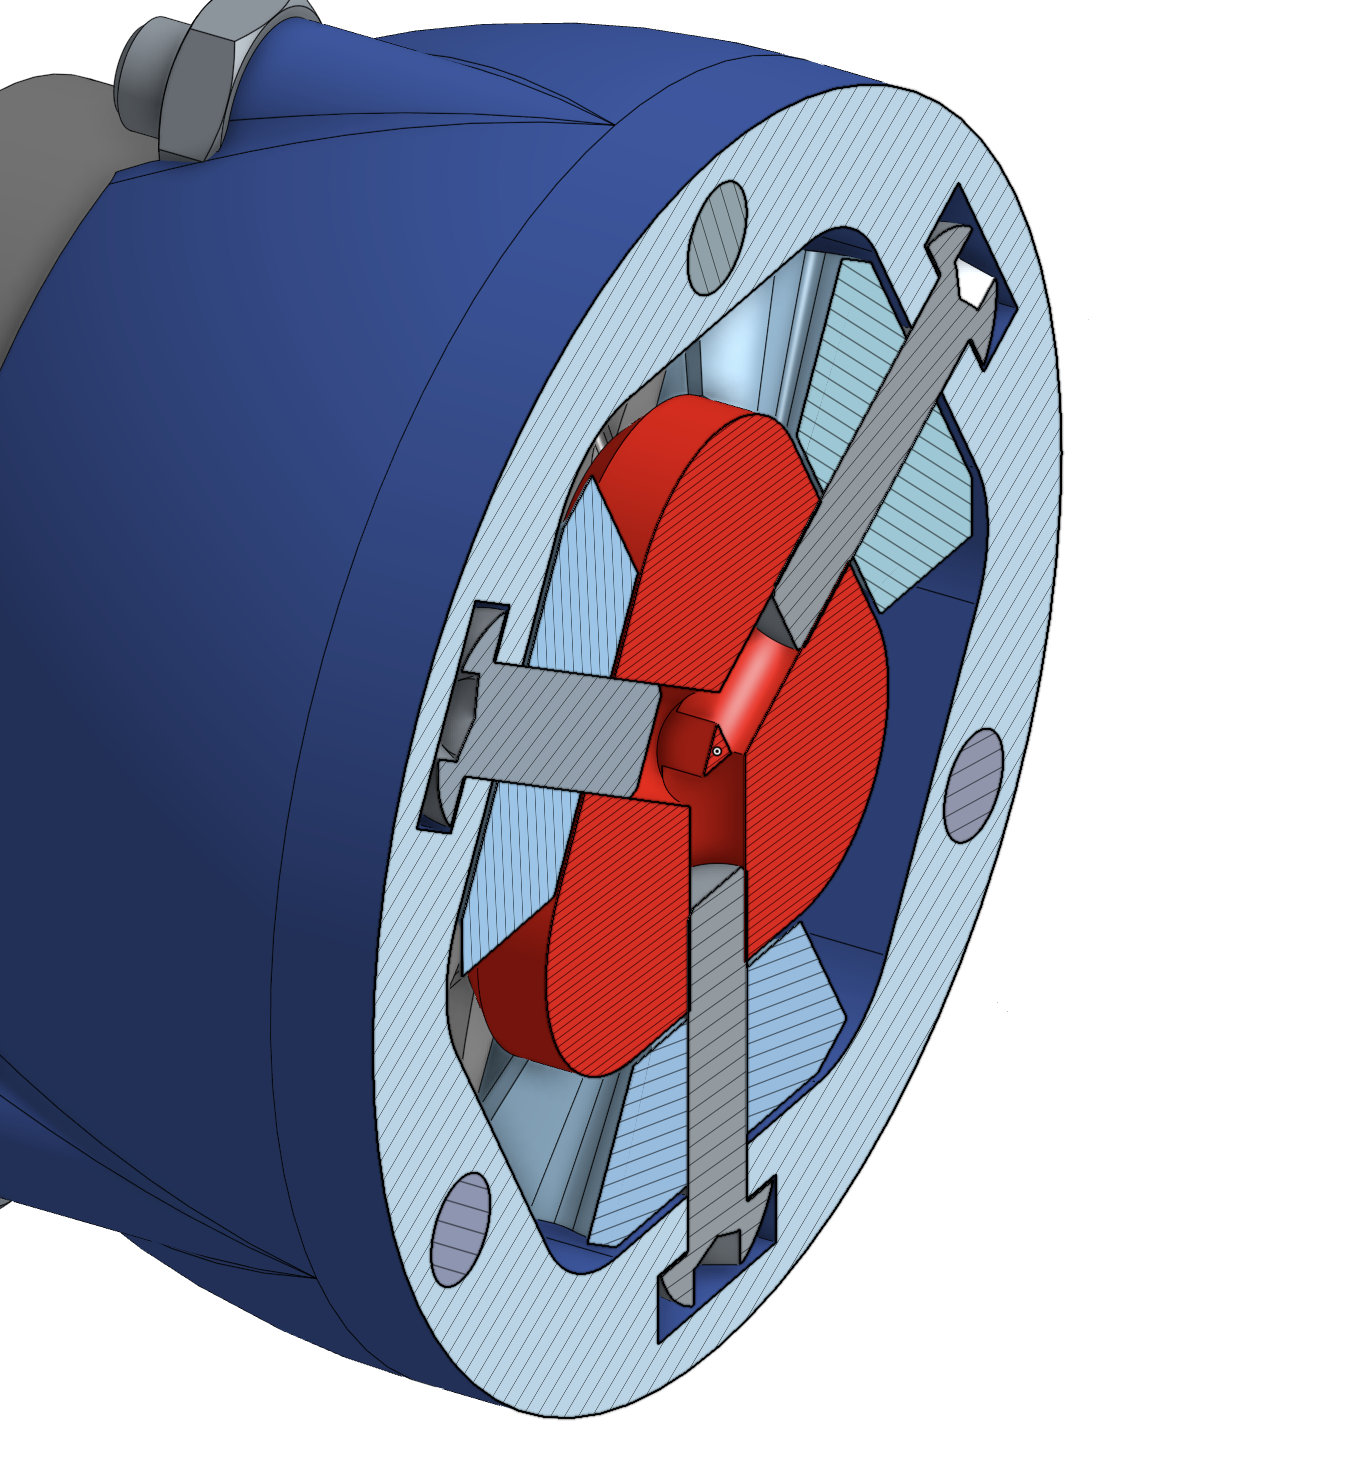
\includegraphics[width=\linewidth, height=0.4\textheight, keepaspectratio]{img/diff_sc_2.png}
        \caption{The Spider Center in Action.}
        \label{fig:diff_sc_2}
    \end{subfigure}
    
    \caption{The Spider Center.}
    \label{fig:C_DG_SC}
\end{figure}

\subsubsection*{Housing}

The housing for the differential gears consists of $2$ halves, the left half and the right half. The two halves are connected by $3$ M$3 \times 30$mm screws and M$3$ nuts (See Figure \ref{fig:C_DG_Assem}). \\

The housing not only houses the gears but also $2 \times$ 6901ZZ bearings (Figure \ref{fig:roller_bearing}). This is to decouple the rotation of the main gears with the rotation of the housing when the two axles are spinning at different speeds. The left housing and the right housing are nearly identical. The left housing houses the bevel gear ring needed to rotate the differential housing using the motor. That gear has $28$ teeth, a module of $1.5$mm and a bevel angle of $70^{\circ}$. In Figure \ref{fig:C_DG_H}, the left housing is the one in light blue and the right housing is in dark blue. The bearings sit inside the housing. \\

The part is printed with the center surface of each of the half facing down. Looking carefully, a chamfer is  present on the end where the bearings sit. This allows for the overhangs to be managed better. It is printed at a layer height of $0.12$mm, has $3$ perimeters and a $25\%$ infill. A brim is used to aid with bed adhesion. 

\begin{figure}[H]
    \centering
    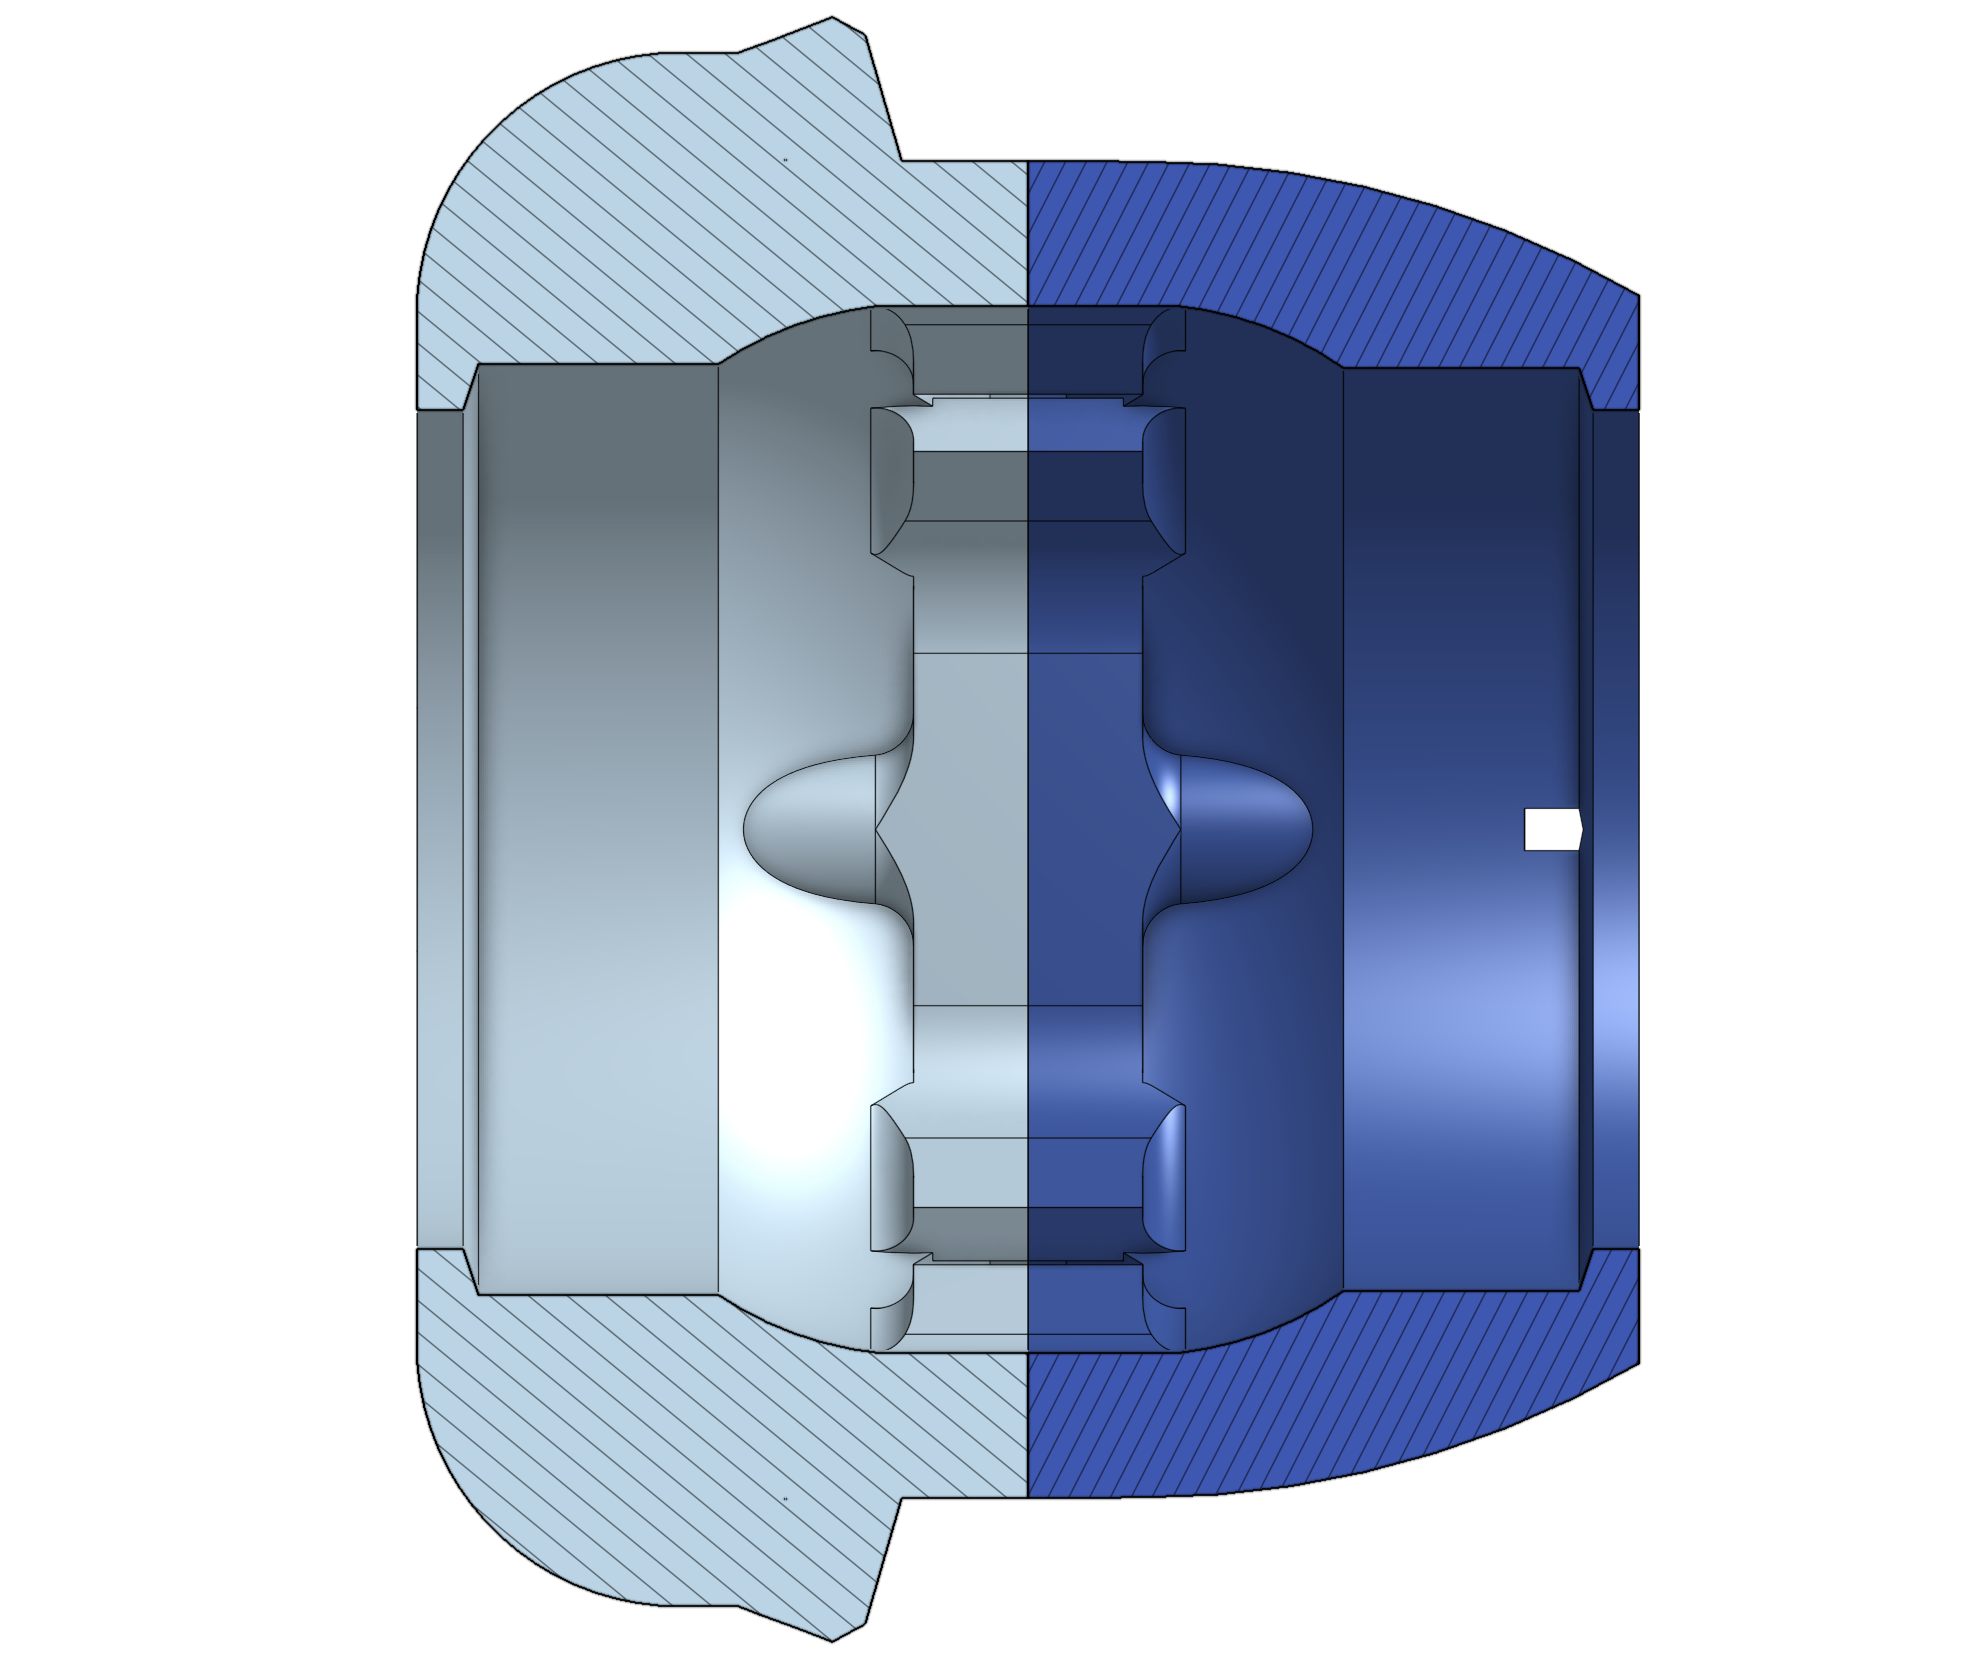
\includegraphics[width=.6\textwidth]{img/diff_housing.png}
    \caption{The Housing for the Gearbox.}
    \label{fig:C_DG_H} 
\end{figure}

\subsubsection*{The Attaching Cups}

The Cup is the part that interfaces with main gear and the $\diameter 12$mm carbon fiber tube that serves as the rear axle. It has the same mounting patter as the Main gear ($6$mm spacing between the 2 M$3$ screws). The Cup extends the $12$mm cylinder outward to house the $12$mm rod. It also has $2 \times \diameter 2$mm holes at each end to interface with the axle and transfer the load. \\

For printing, the cup is split into 2 parts axially (see Figure \ref{fig:C_DG_C}) and then printed flat to ensure the force moves along the layers and ensure ease of printability. It is printed at a layer height of $0.12$mm, has $3$ perimeters and a $25\%$ infill. A brim is used to aid with bed adhesion. 

\begin{figure}[H]
    \centering
    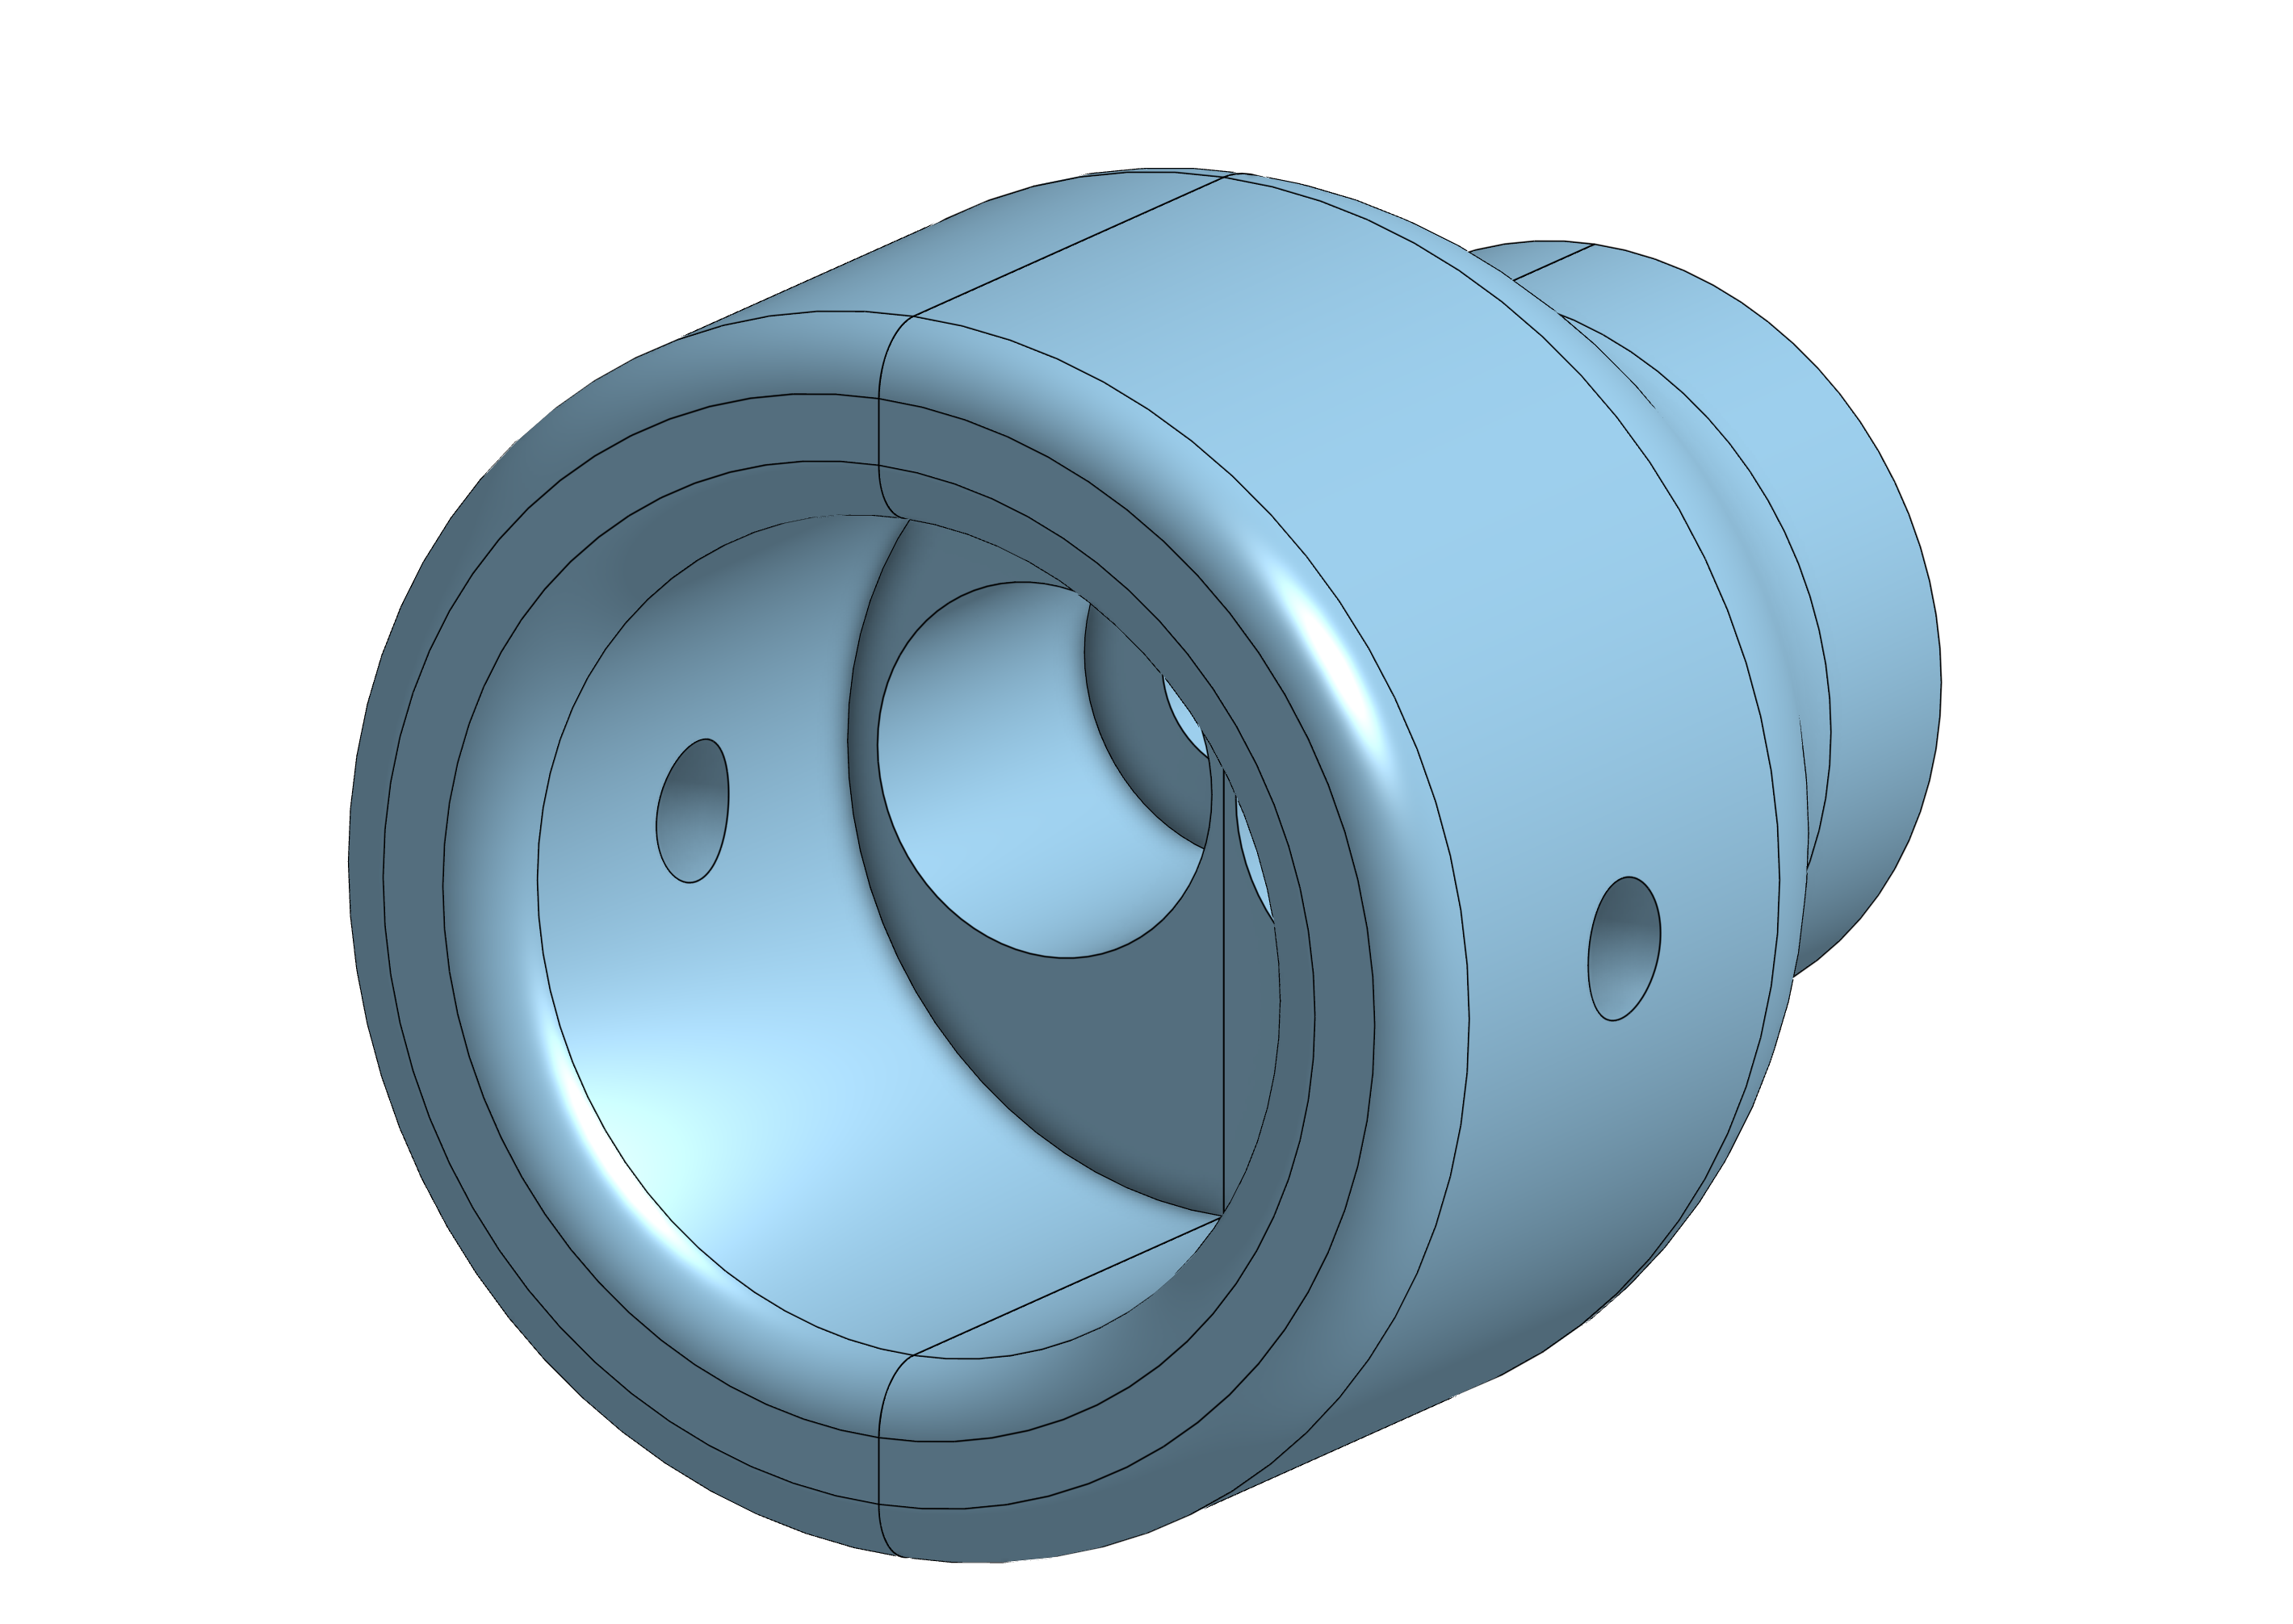
\includegraphics[width=.6\textwidth]{img/cup.png}
    \caption{The Attaching Cup.}
    \label{fig:C_DG_C} 
\end{figure}

\subsubsection*{The Spacer}

When looking at Figure \ref{fig:C_DG_Assem}, one can see that there are bearings on the outside as well, excluding the ones inside the housing. These are also 6901ZZ bearings and are responsible for the rotation of the housing itself. They are clamped from either end (discussed later). To ensure that there is $\rightarrow$
\begin{enumerate}
\item No play in the mounting of the differential gearbox
\item Adequate separation between the bearing ends and the housing of the wall
\item Ease of motion
\end{enumerate}
A spacer disk is mounted in between the two bearings. This disk also provides the pre-load needed in the gearbox stackup. It also ensures that the main gears in the differential mesh properly with the spider gears. Unlike the TPU spacer (Figure \ref{fig:C_TPUS}), this is made out of PLA. \\

It is printed at a layer height of $0.12$mm, has $3$ perimeters and a $25\%$ infill. A brim is used to aid with bed adhesion. The height of the disk, nominally $2.00$mm can be adjusted to adjust the pre-load. The grove of the roller bearing (Figure \ref{fig:roller_bearing}). The disk has an outer diameter of $16.40$mm and an inner diameter of $12.4$mm. You can see the orange disk in Figure \ref{fig:C_DG_Spacer} doing its job.

\begin{figure}[H]
    \centering
    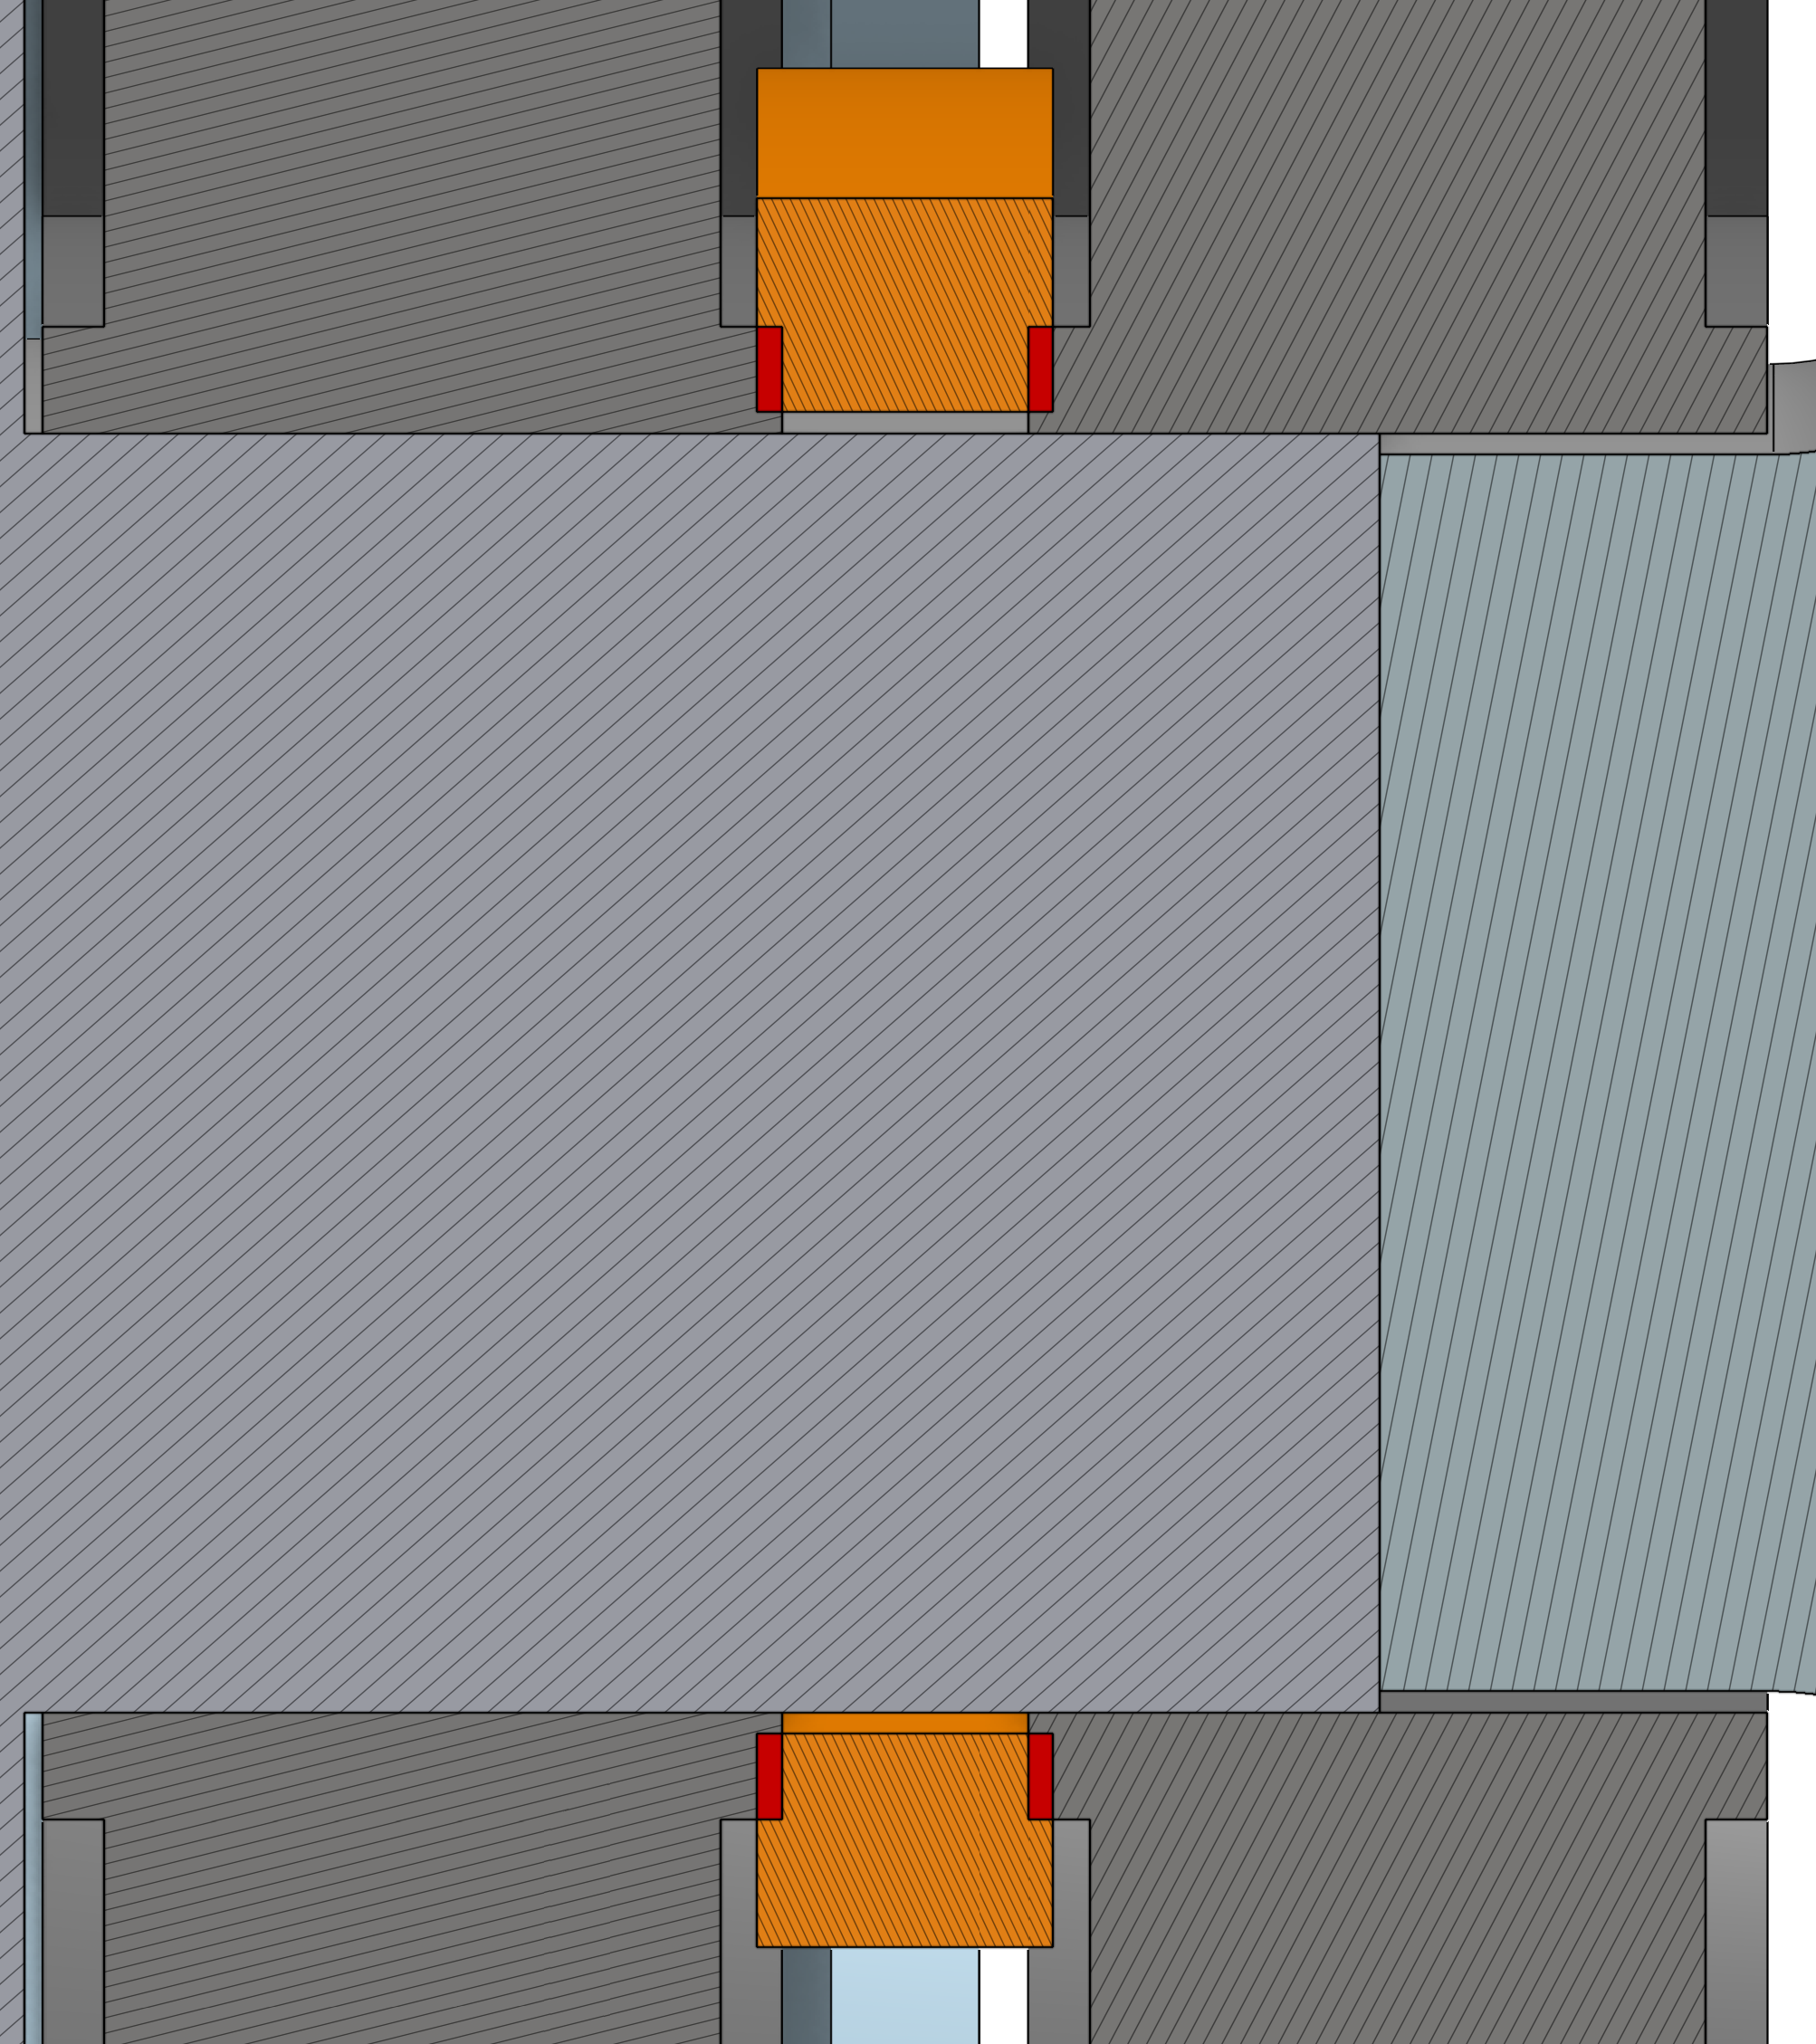
\includegraphics[width=.6\textwidth]{img/diff_spacer.png}
    \caption{The Spacer Disk.}
    \label{fig:C_DG_Spacer} 
\end{figure}

\subsection{The Rear Axle}

The rear axle is what really brings everything together. The mounts for the rear axle hold the motor, the batteries, the needle roller bearings and the differential. They are also the end point of the 4 carbon fiber rods used to strengthen the vehicle. The parts for the rear axle are also among the largest parts. \\

The rear axle houses the 2 BCWN-T-d12-IR bearings (Figure \ref{fig:needle_roller_bearing}). We start our journey with the Rear Axle Mount. It encompasses the whole rear axle and only consists of 2 parts that work in tandem.

\begin{figure}[H]
    \centering
    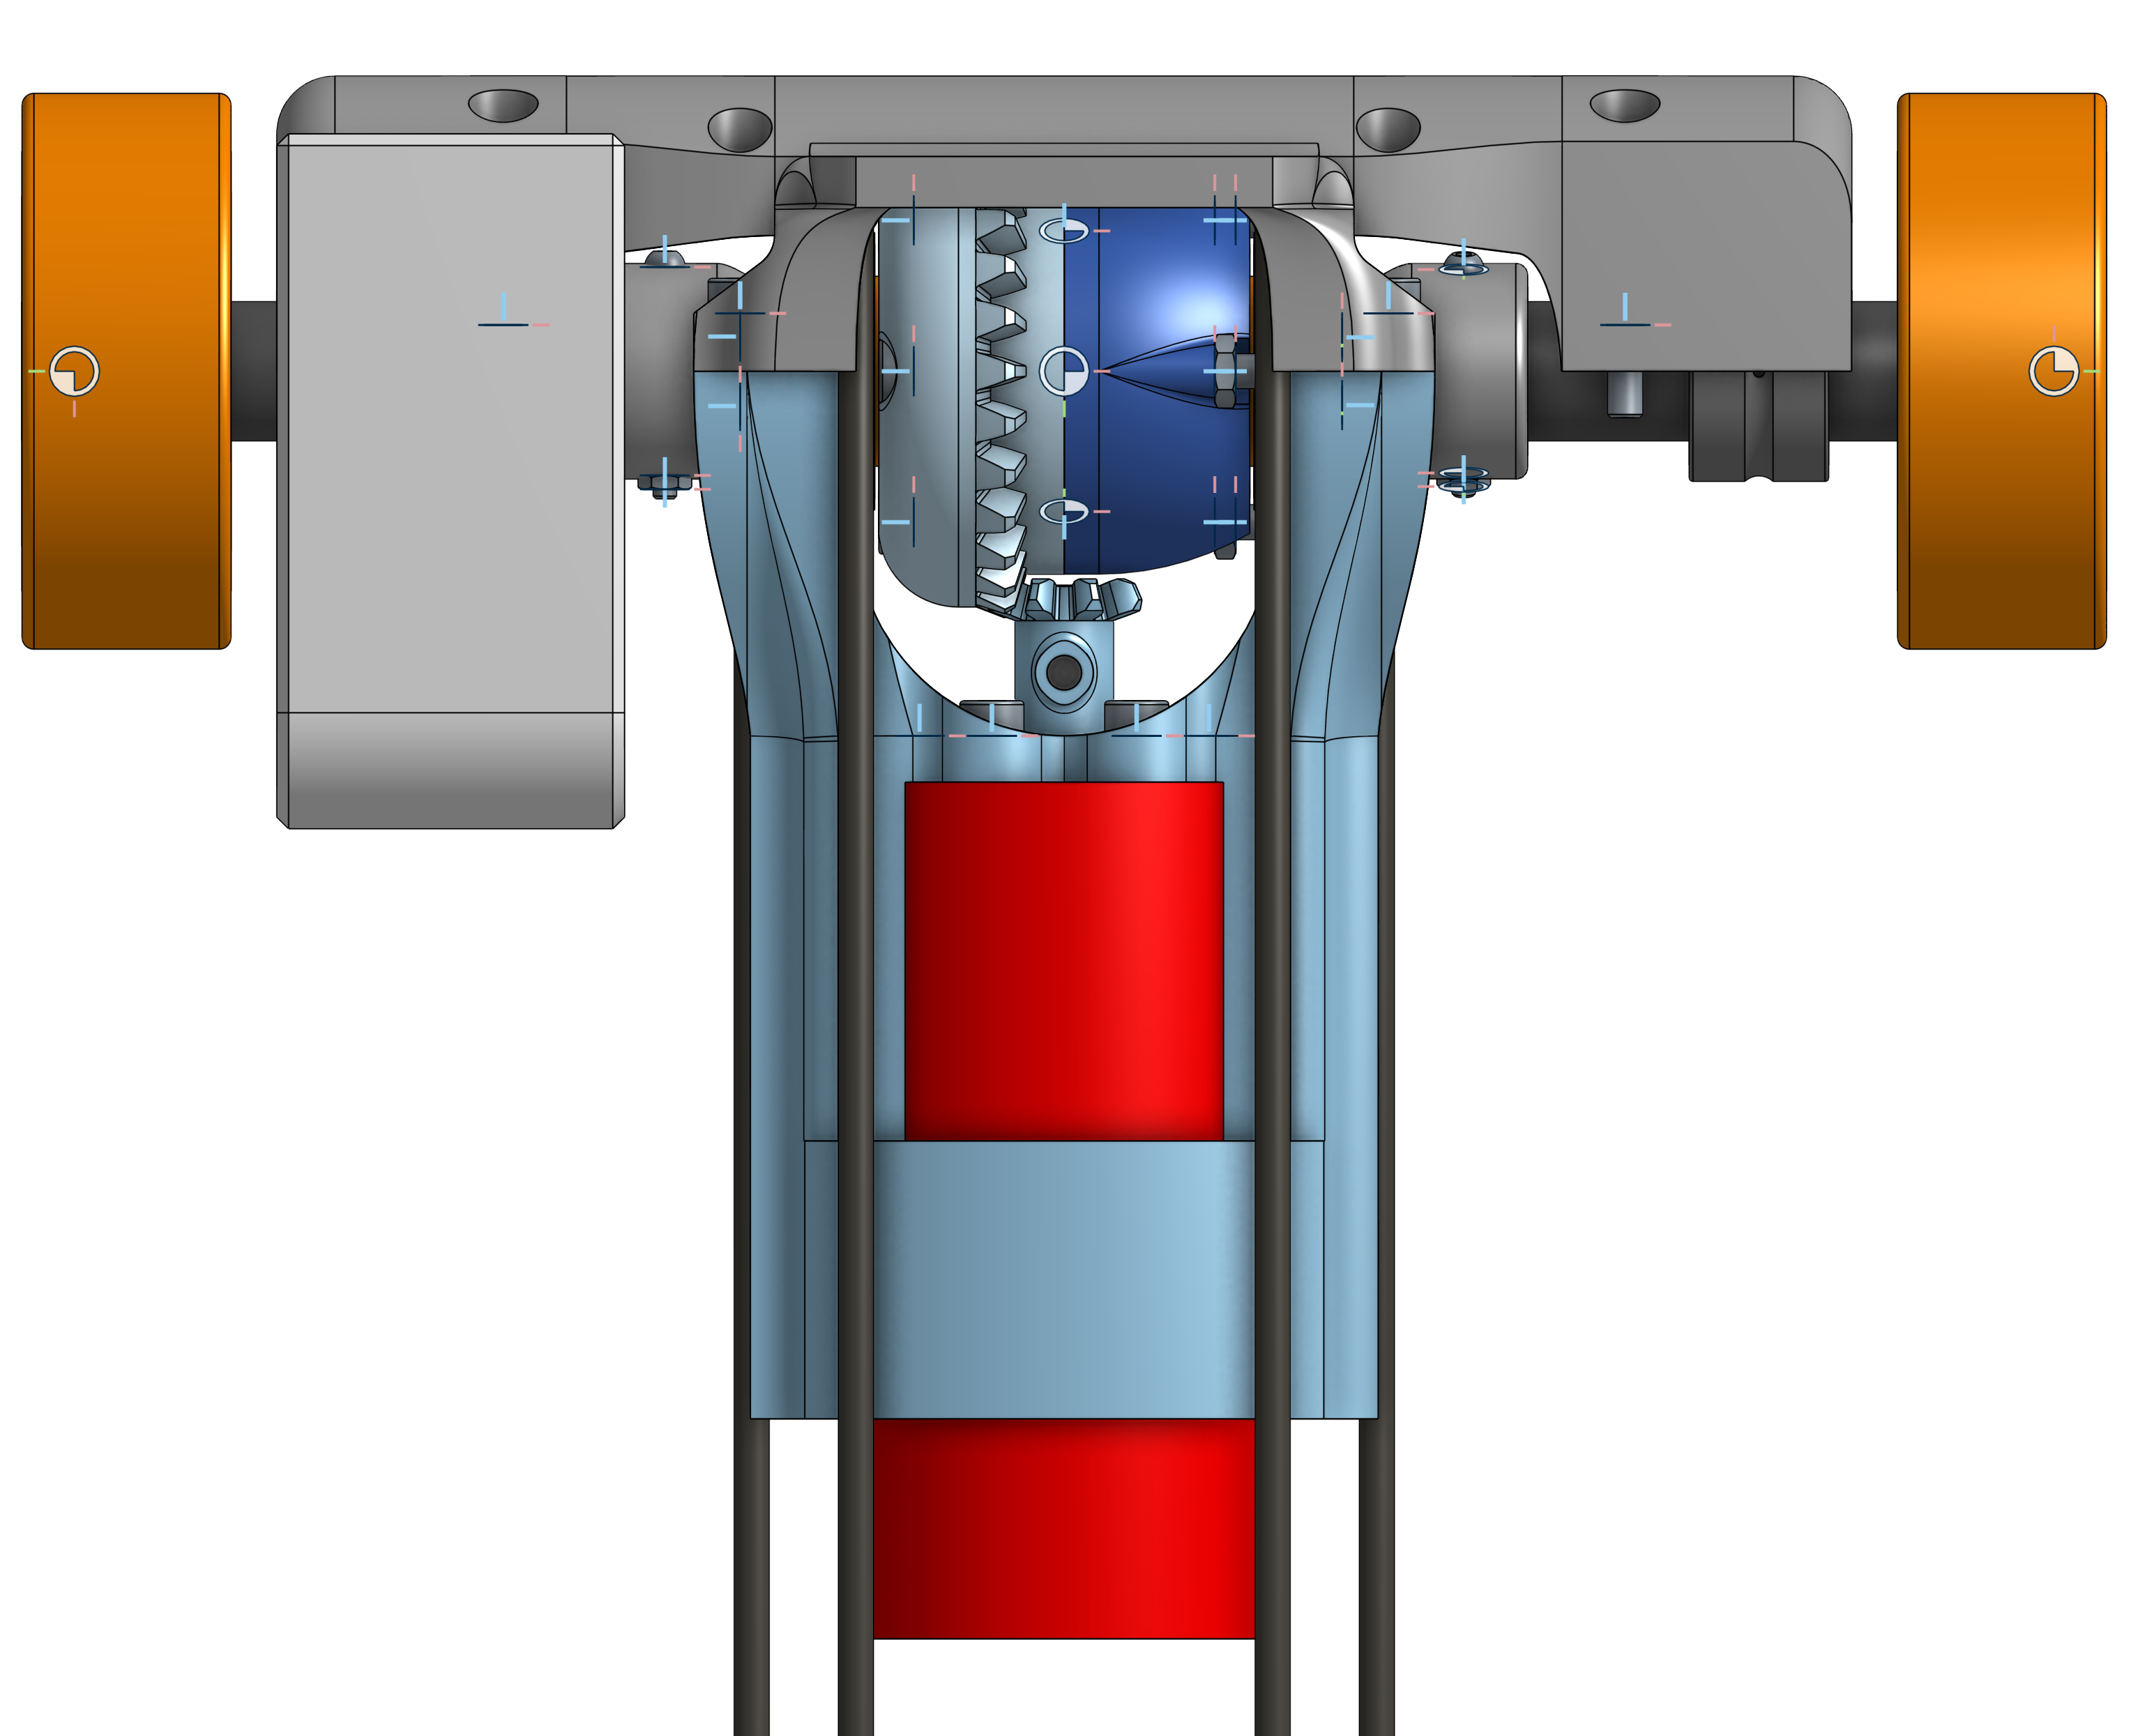
\includegraphics[width=.8\textwidth]{img/rear_assem.png}
    \caption{The Rear Axle Assembly.}
    \label{fig:C_R_Assem} 
\end{figure}

\subsubsection*{Rear Axle Mount Front}

The front mount is the light blue colored part in Figure \ref{fig:C_R_Assem}. It houses the motor and serves as one half of the gearbox mount. It is one of the most complex parts. \\

It houses holes for $6$ M$3 \times 8$mm screws that connect the motor to the mount. It also has space for $4$ M$3 \times 4$mm heat set inserts at the very end to interface with the back mount and space for $6$ M$3 \times 6$mm heat set inserts, $3$ on each side (see Figure \ref{fig:C_R_FM}) that allow it to interface with the parts that connect the front and the rear axle. The front mount also serves as the end point of the bottom set of $\diameter 3$mm rods. \\

The part is printed with the forward facing face in Figure \ref{fig:C_R_Assem} pointing down, as shown in Figure \ref{fig:C_R_FM_P}. The part does need supports at the area where the motor mounts. It is printed at a layer height of $0.20$mm, has $3$ perimeters and a $25\%$ infill. A brim is used to aid with bed adhesion.

\begin{figure}[H]
    \centering
    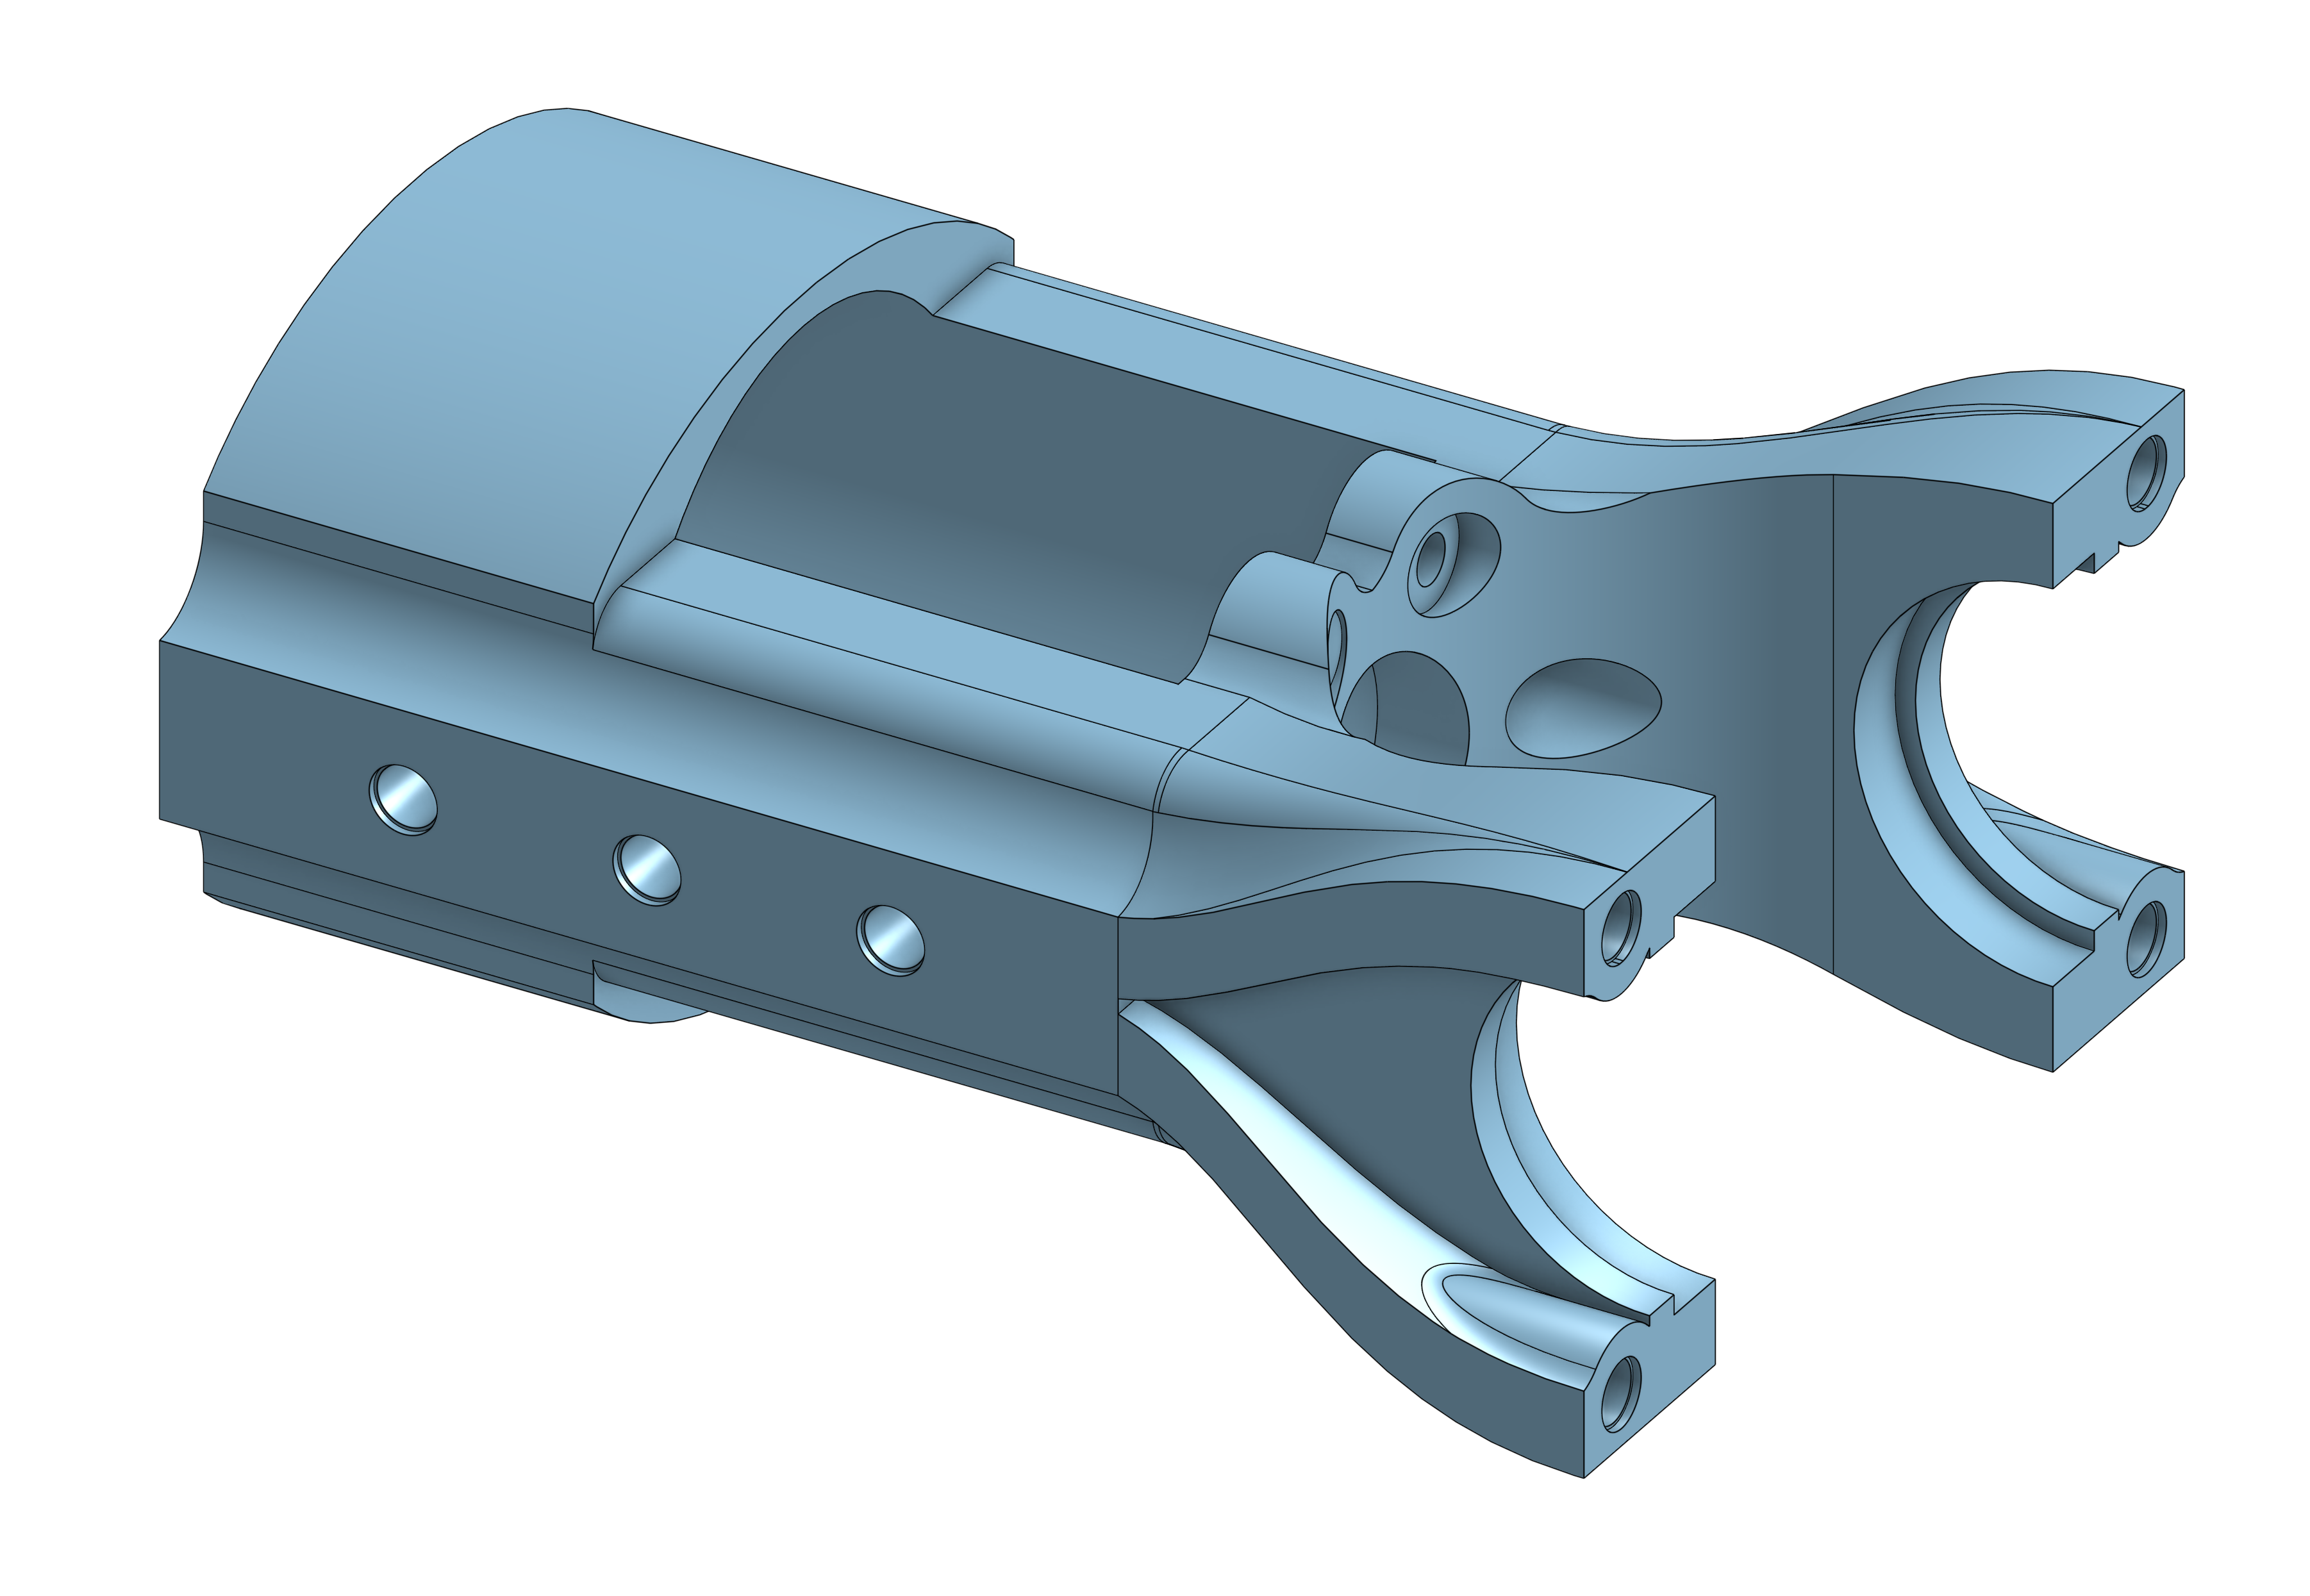
\includegraphics[width=.8\textwidth]{img/rear_fmount.png}
    \caption{The Front Mount.}
    \label{fig:C_R_FM} 
\end{figure}

\begin{figure}[H]
    \centering
    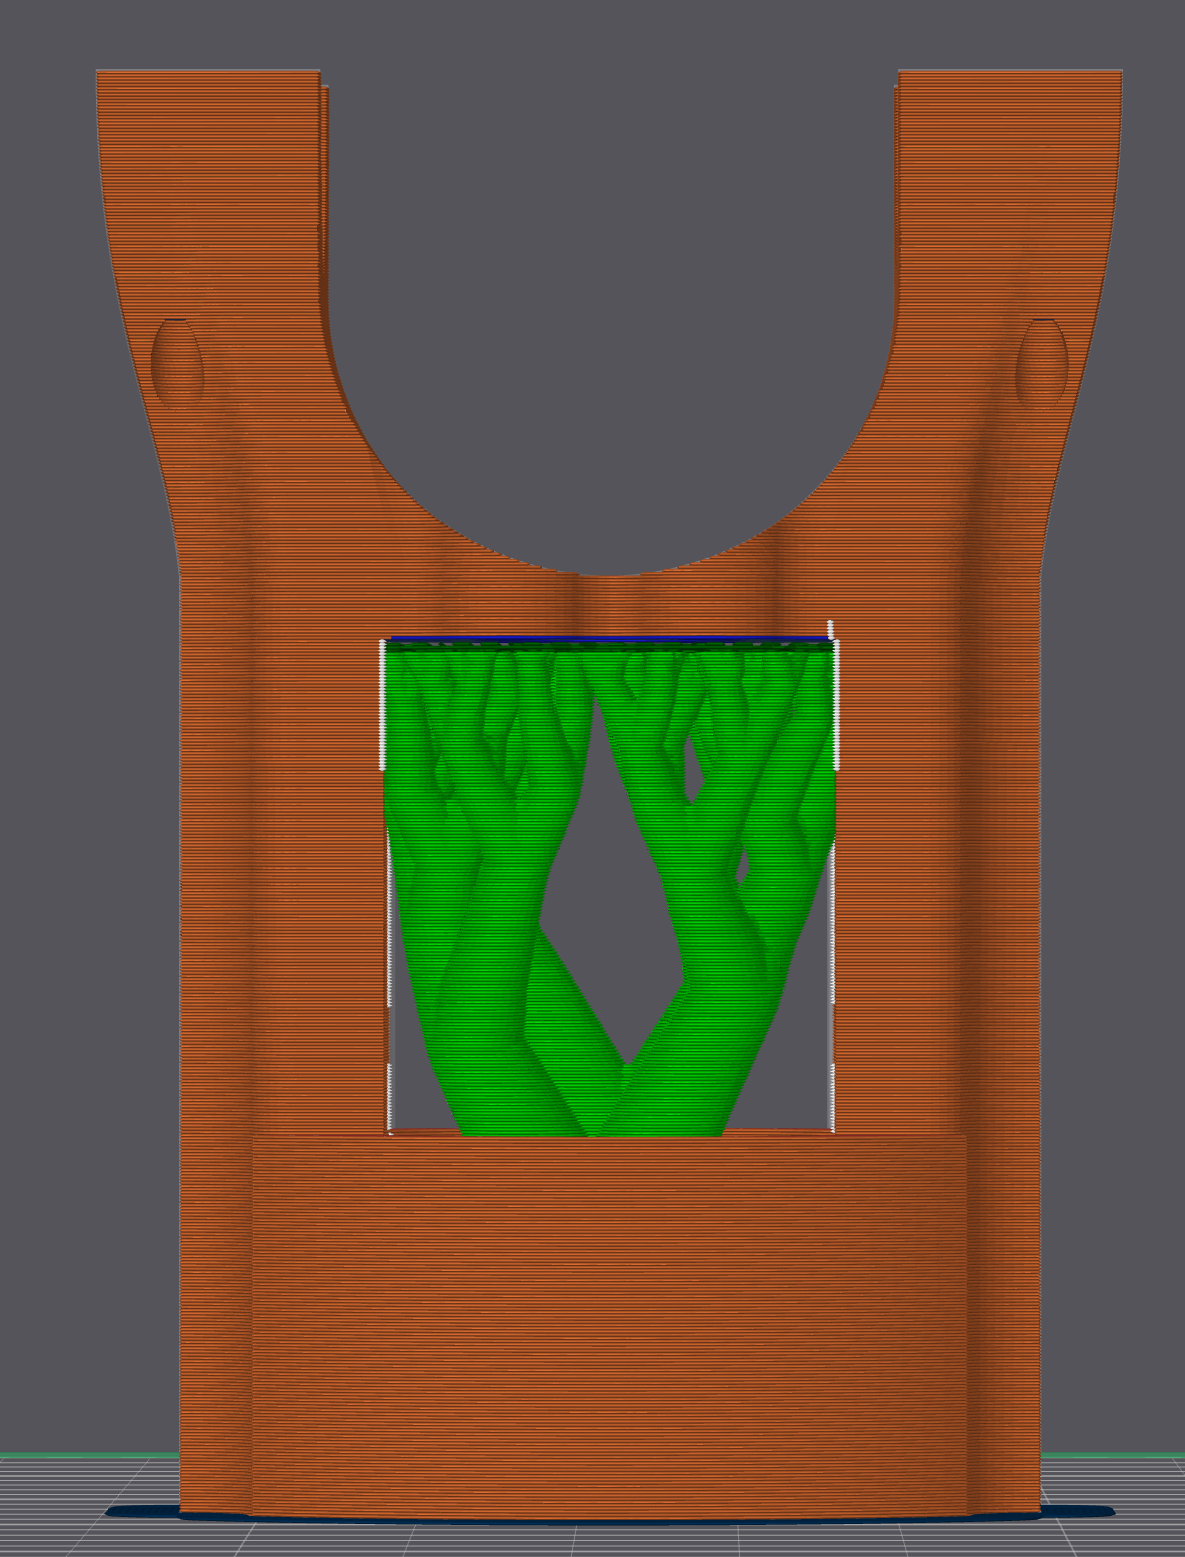
\includegraphics[width=.5\textwidth]{img/rear_fmount_print.png}
    \caption{The Front Mount in the Slicer.}
    \label{fig:C_R_FM_P} 
\end{figure}

\subsubsection*{Rear Axle Mount Rear}

The rear mount serves as a half to mount the BCWN-T-d12-IR as well as the 6901ZZ bearings. It's a fairly chunky piece. It uses 8 M$3 \times 8$mm screws that interface with the rest of the vehicle. This part serves as the end mount of the top $\diameter 3$mm carbon fiber rods. \\

The part prints with the front face facing downward. It is printed at a layer height of $0.20$mm, has $3$ perimeters and a $25\%$ infill. A brim is used to aid with bed adhesion and prevent warping. Supports are not needed but appreciated. \\

\begin{figure}[H]
    \centering
    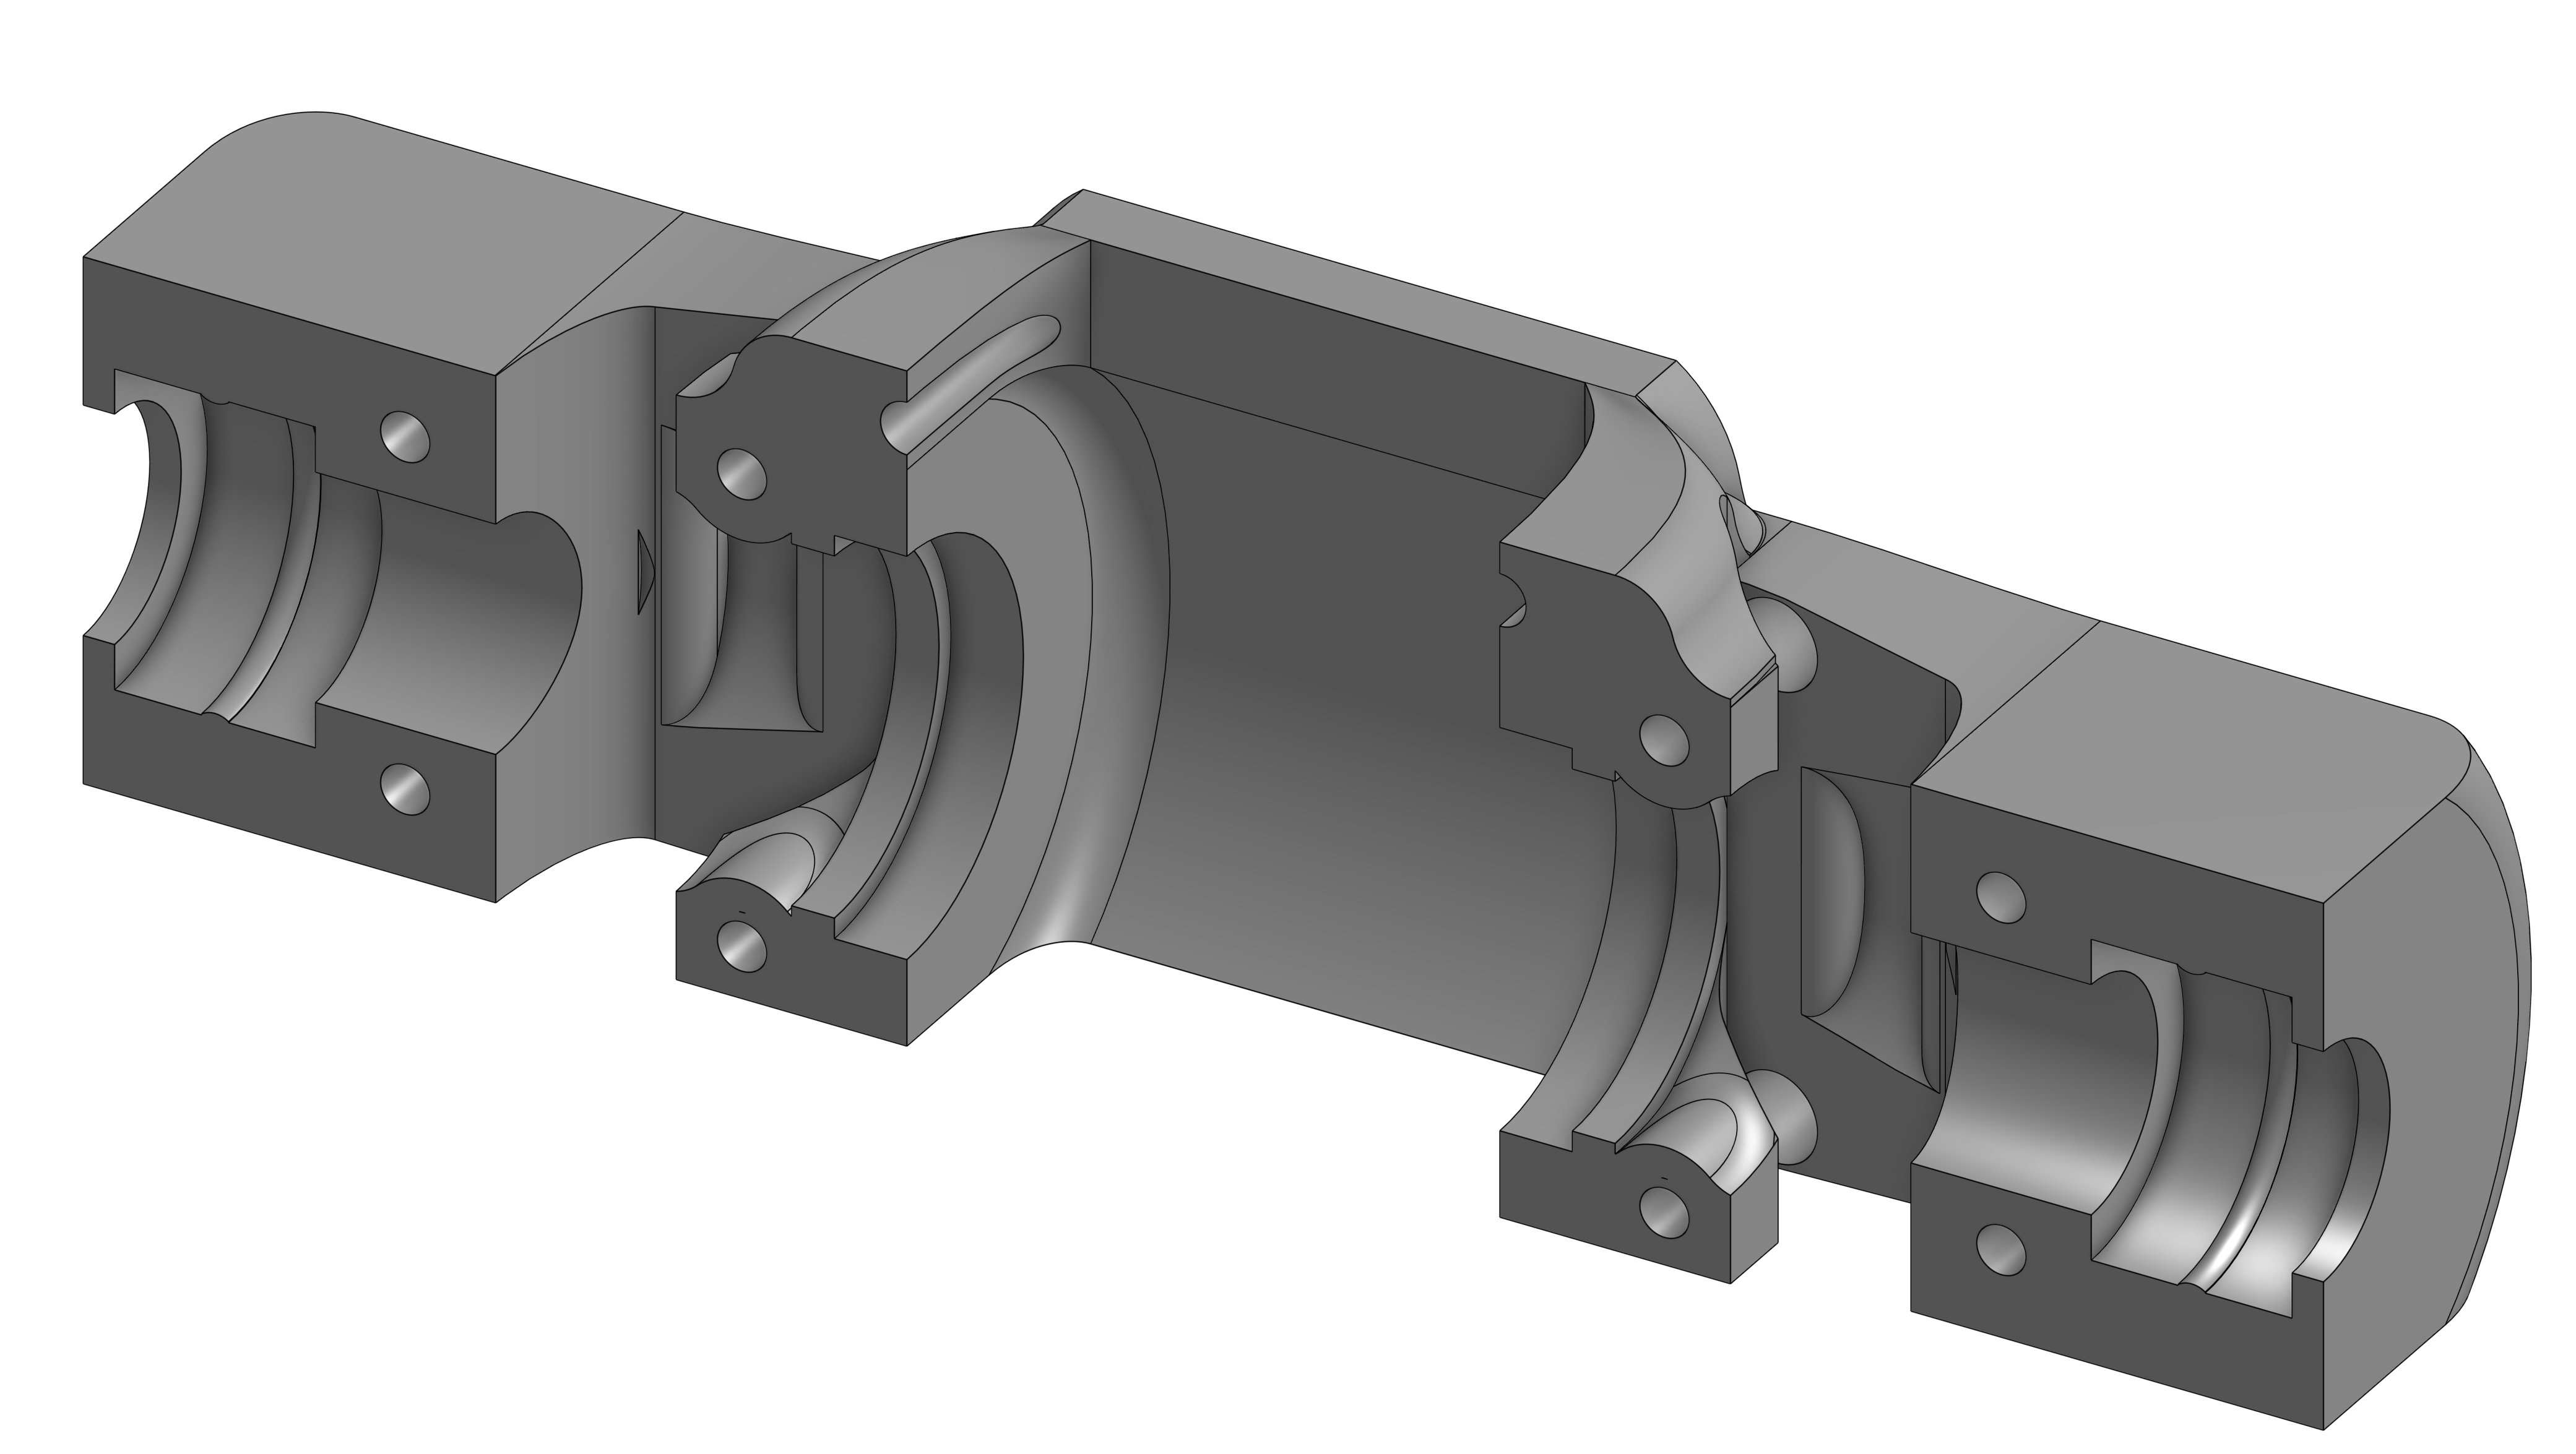
\includegraphics[width=.8\textwidth]{img/rear_bmount.png}
    \caption{The Back Mount.}
    \label{fig:C_R_BM} 
\end{figure}

The batteries mount above the rear axle and are shown in the next section.

\subsection{The Center}

This part ties the the two axles together. It houses the LiDAR, the Raspberry Pi, the ESC and the batteries. 

\begin{figure}[H]
    \centering
    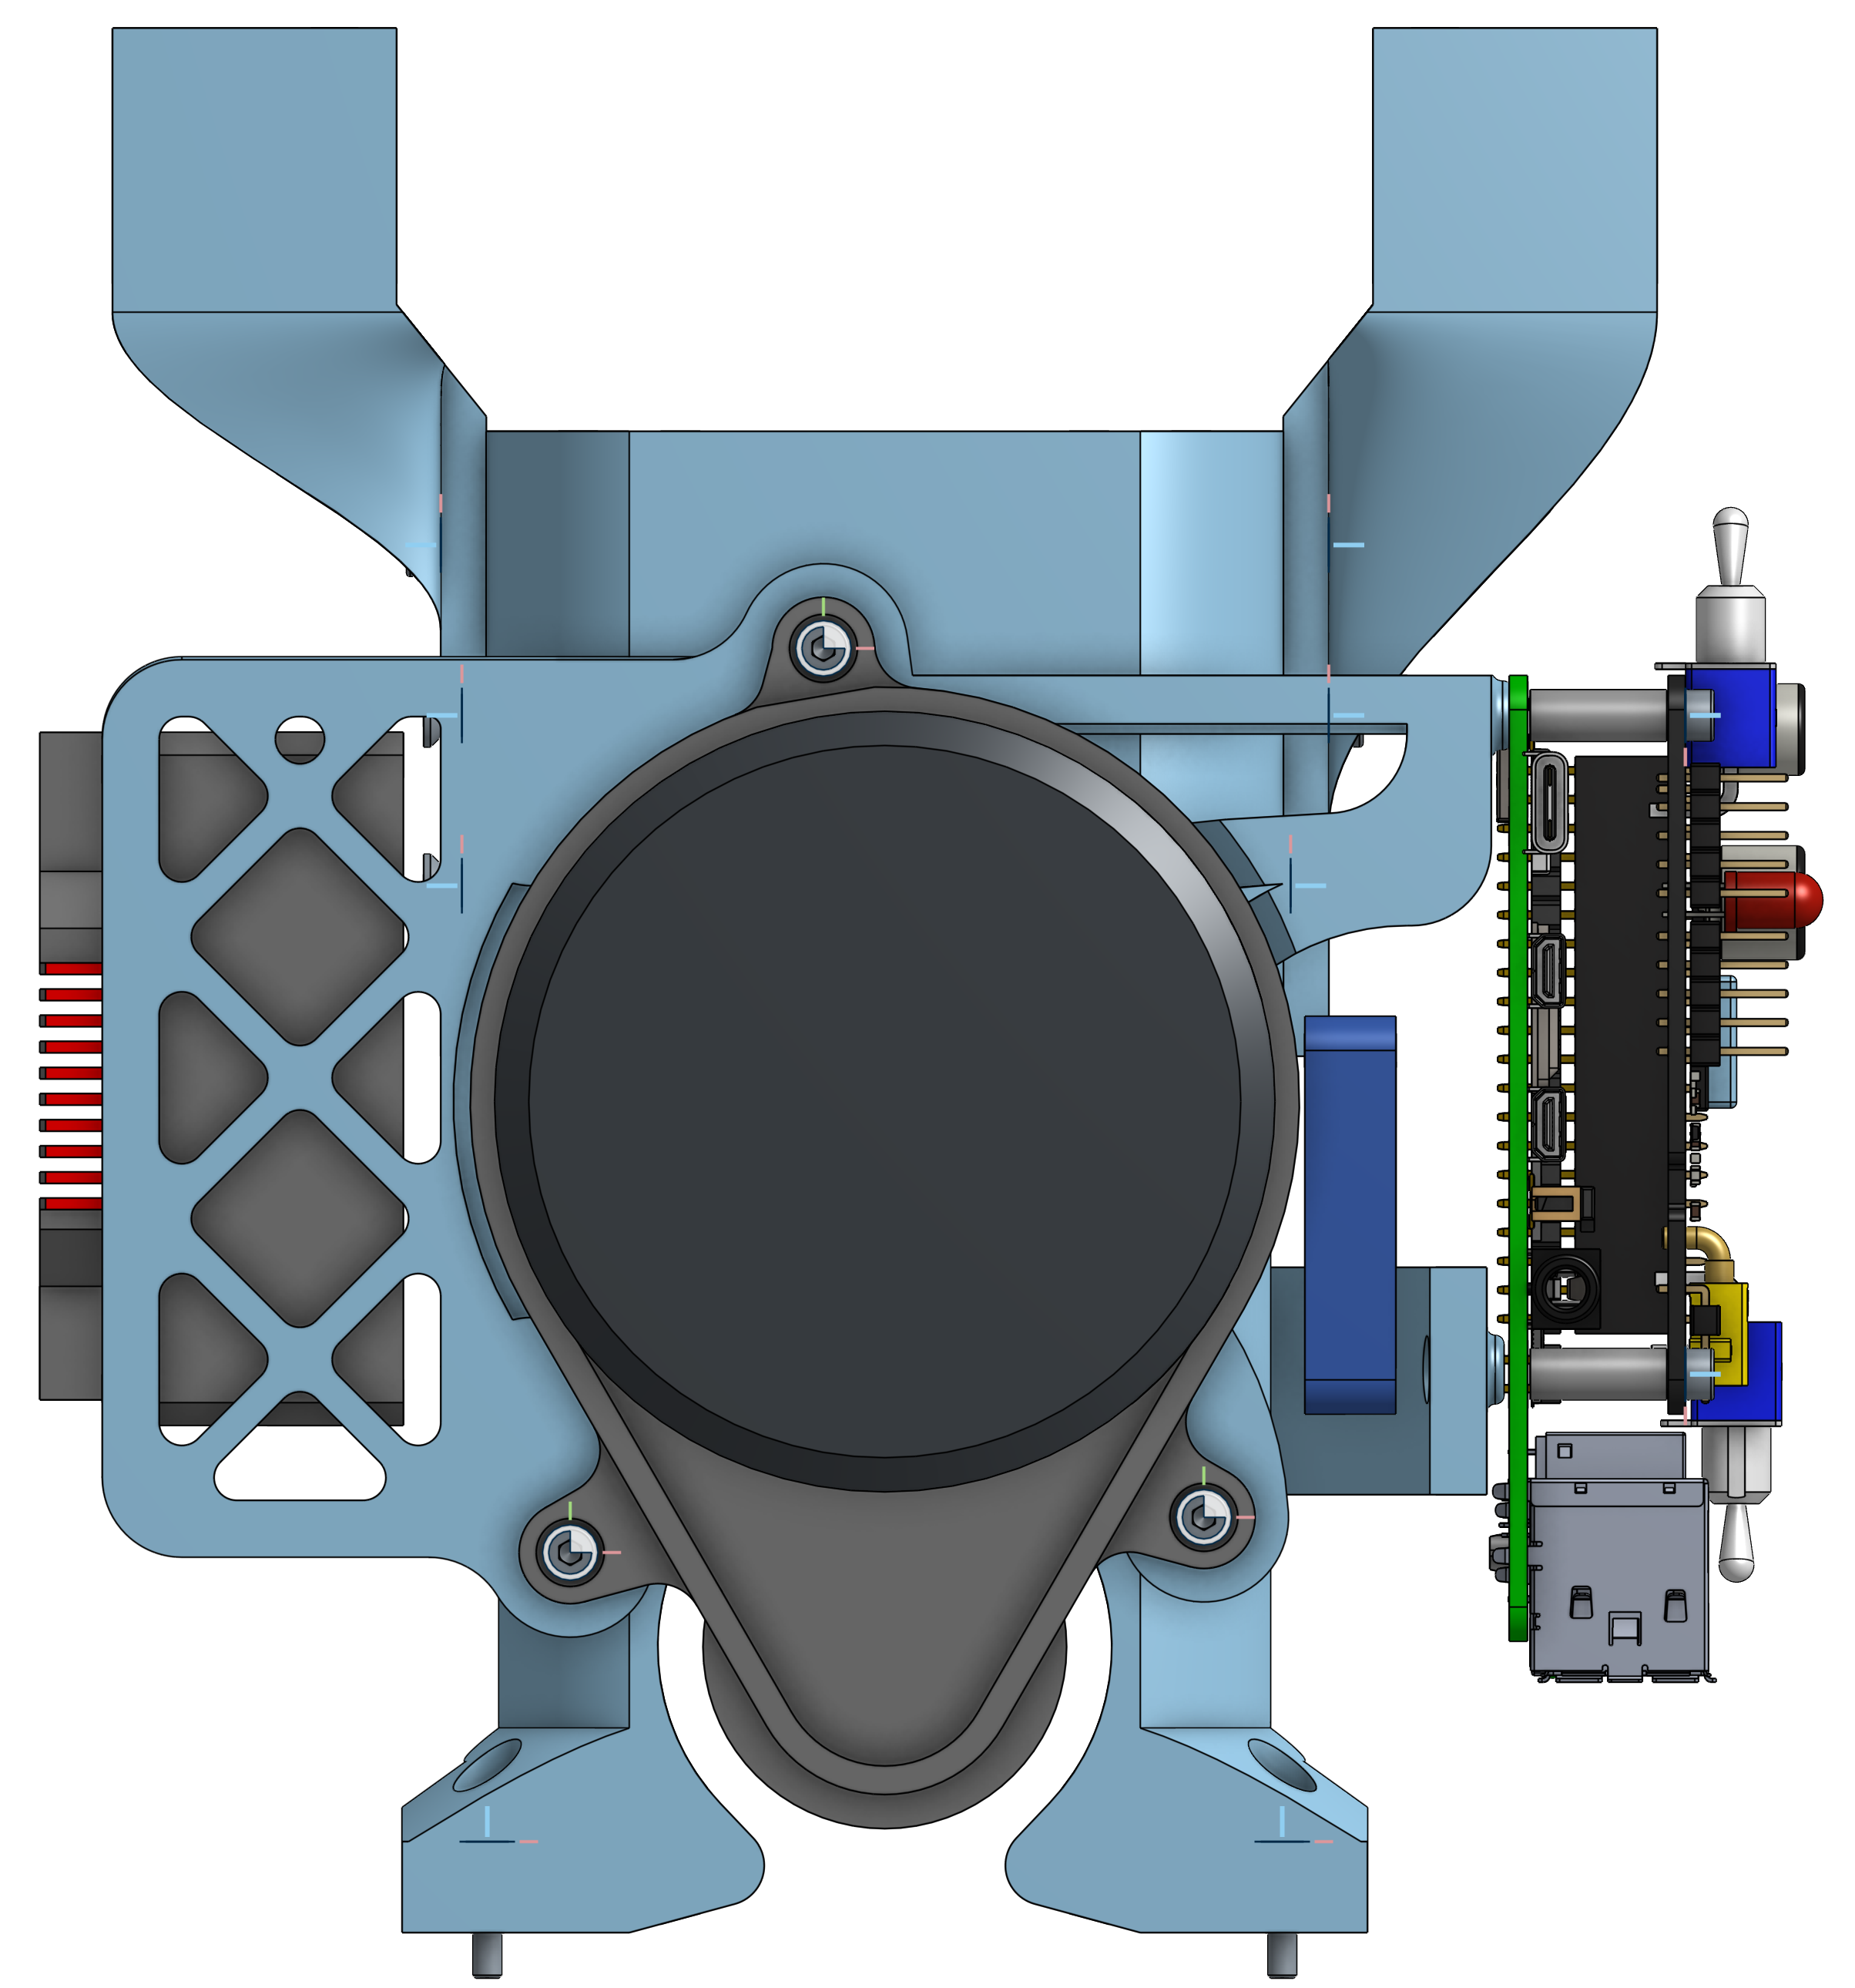
\includegraphics[width=.8\textwidth]{img/center_assem.png}
    \caption{The Center Assembly.}
    \label{fig:C_C_Assem} 
\end{figure}

\subsubsection*{Top Brace}

The top brace is the main part that connects the motor mount to the steering column. The top supporting rods run directly, all the way through this. It is one of the two biggest parts of the entire vehicle. \\

It connects to the motor mount (Rear axle mount front) with $6$ M$3 \time 16$mm screws and connects with the steering mount with $2$ M$3 \times 12$mm screws. It takes $2$ M$3 \times 6$m heat set inserts on the top surface for the LiDAR \& ESC mount. \\

The part is printed with the rear facing surface pointing downward (the part is upright) and does not require any supports. The holes at the front in Figure \ref{fig:C_C_Top} are counter bore, but features are provided to help with printing. PreFlight can also be used to aid with counter bore bridging.

\begin{figure}[H]
    \centering
    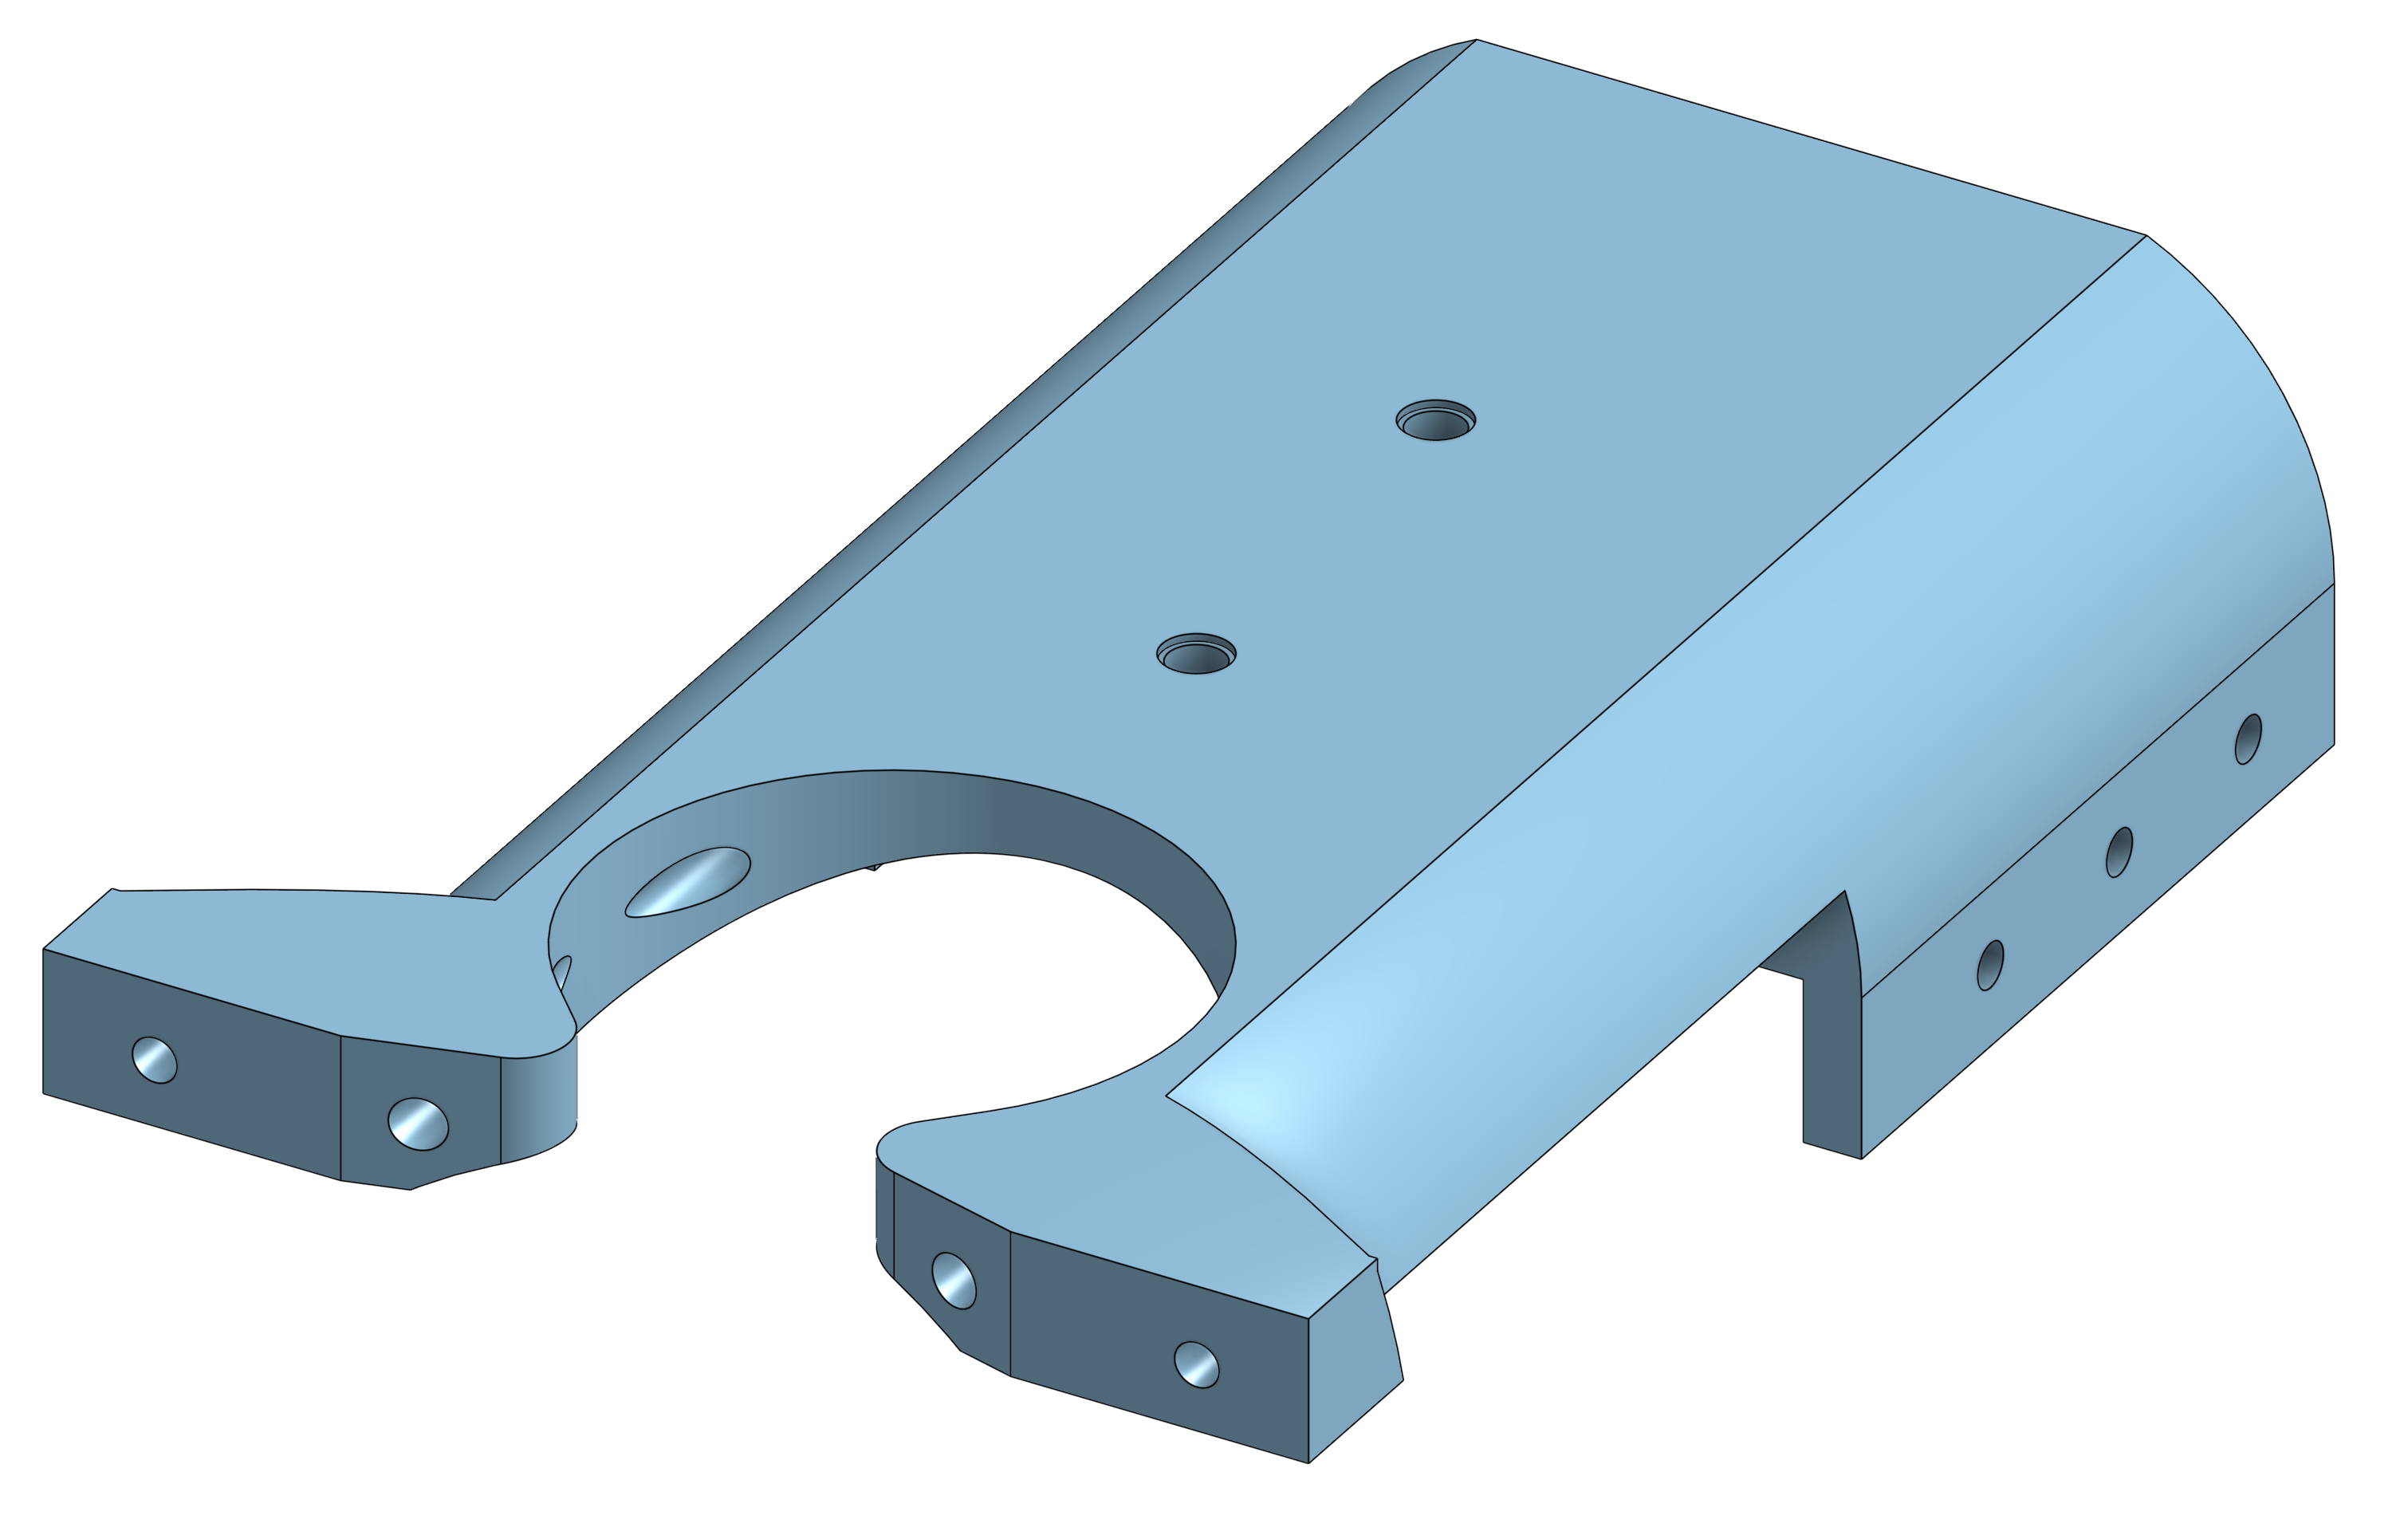
\includegraphics[width=.8\textwidth]{img/top_br.png}
    \caption{The Top Brace.}
    \label{fig:C_C_Top} 
\end{figure}

The part is printed at a layer height of $0.20$mm, has $3$ perimeters and a $25\%$ infill. A brim is used to aid with bed adhesion and prevent the part from peeling off when printing.

\subsubsection*{Bottom Left \& Bottom Right Brace}

The bottom left and bottom right braces are just mirrored parts. They are tiny in comparison to the top brace. They help with connecting the top brace to the bottom pair of carbon fiber rods. They also interface with the motor mount (Rear axle mount front) on the same $6$ points as the top brace. They are wedged between the motor mount and the top brace. \\

They are printed with either of the end, flat, sides pointing down. They do not need supports and are printed at a layer height of $0.20$mm, has $3$ perimeters and a $25\%$ infill. A brim is used to aid with bed adhesion and prevent the part from peeling off when printing.

\begin{figure}[H]
    \centering
    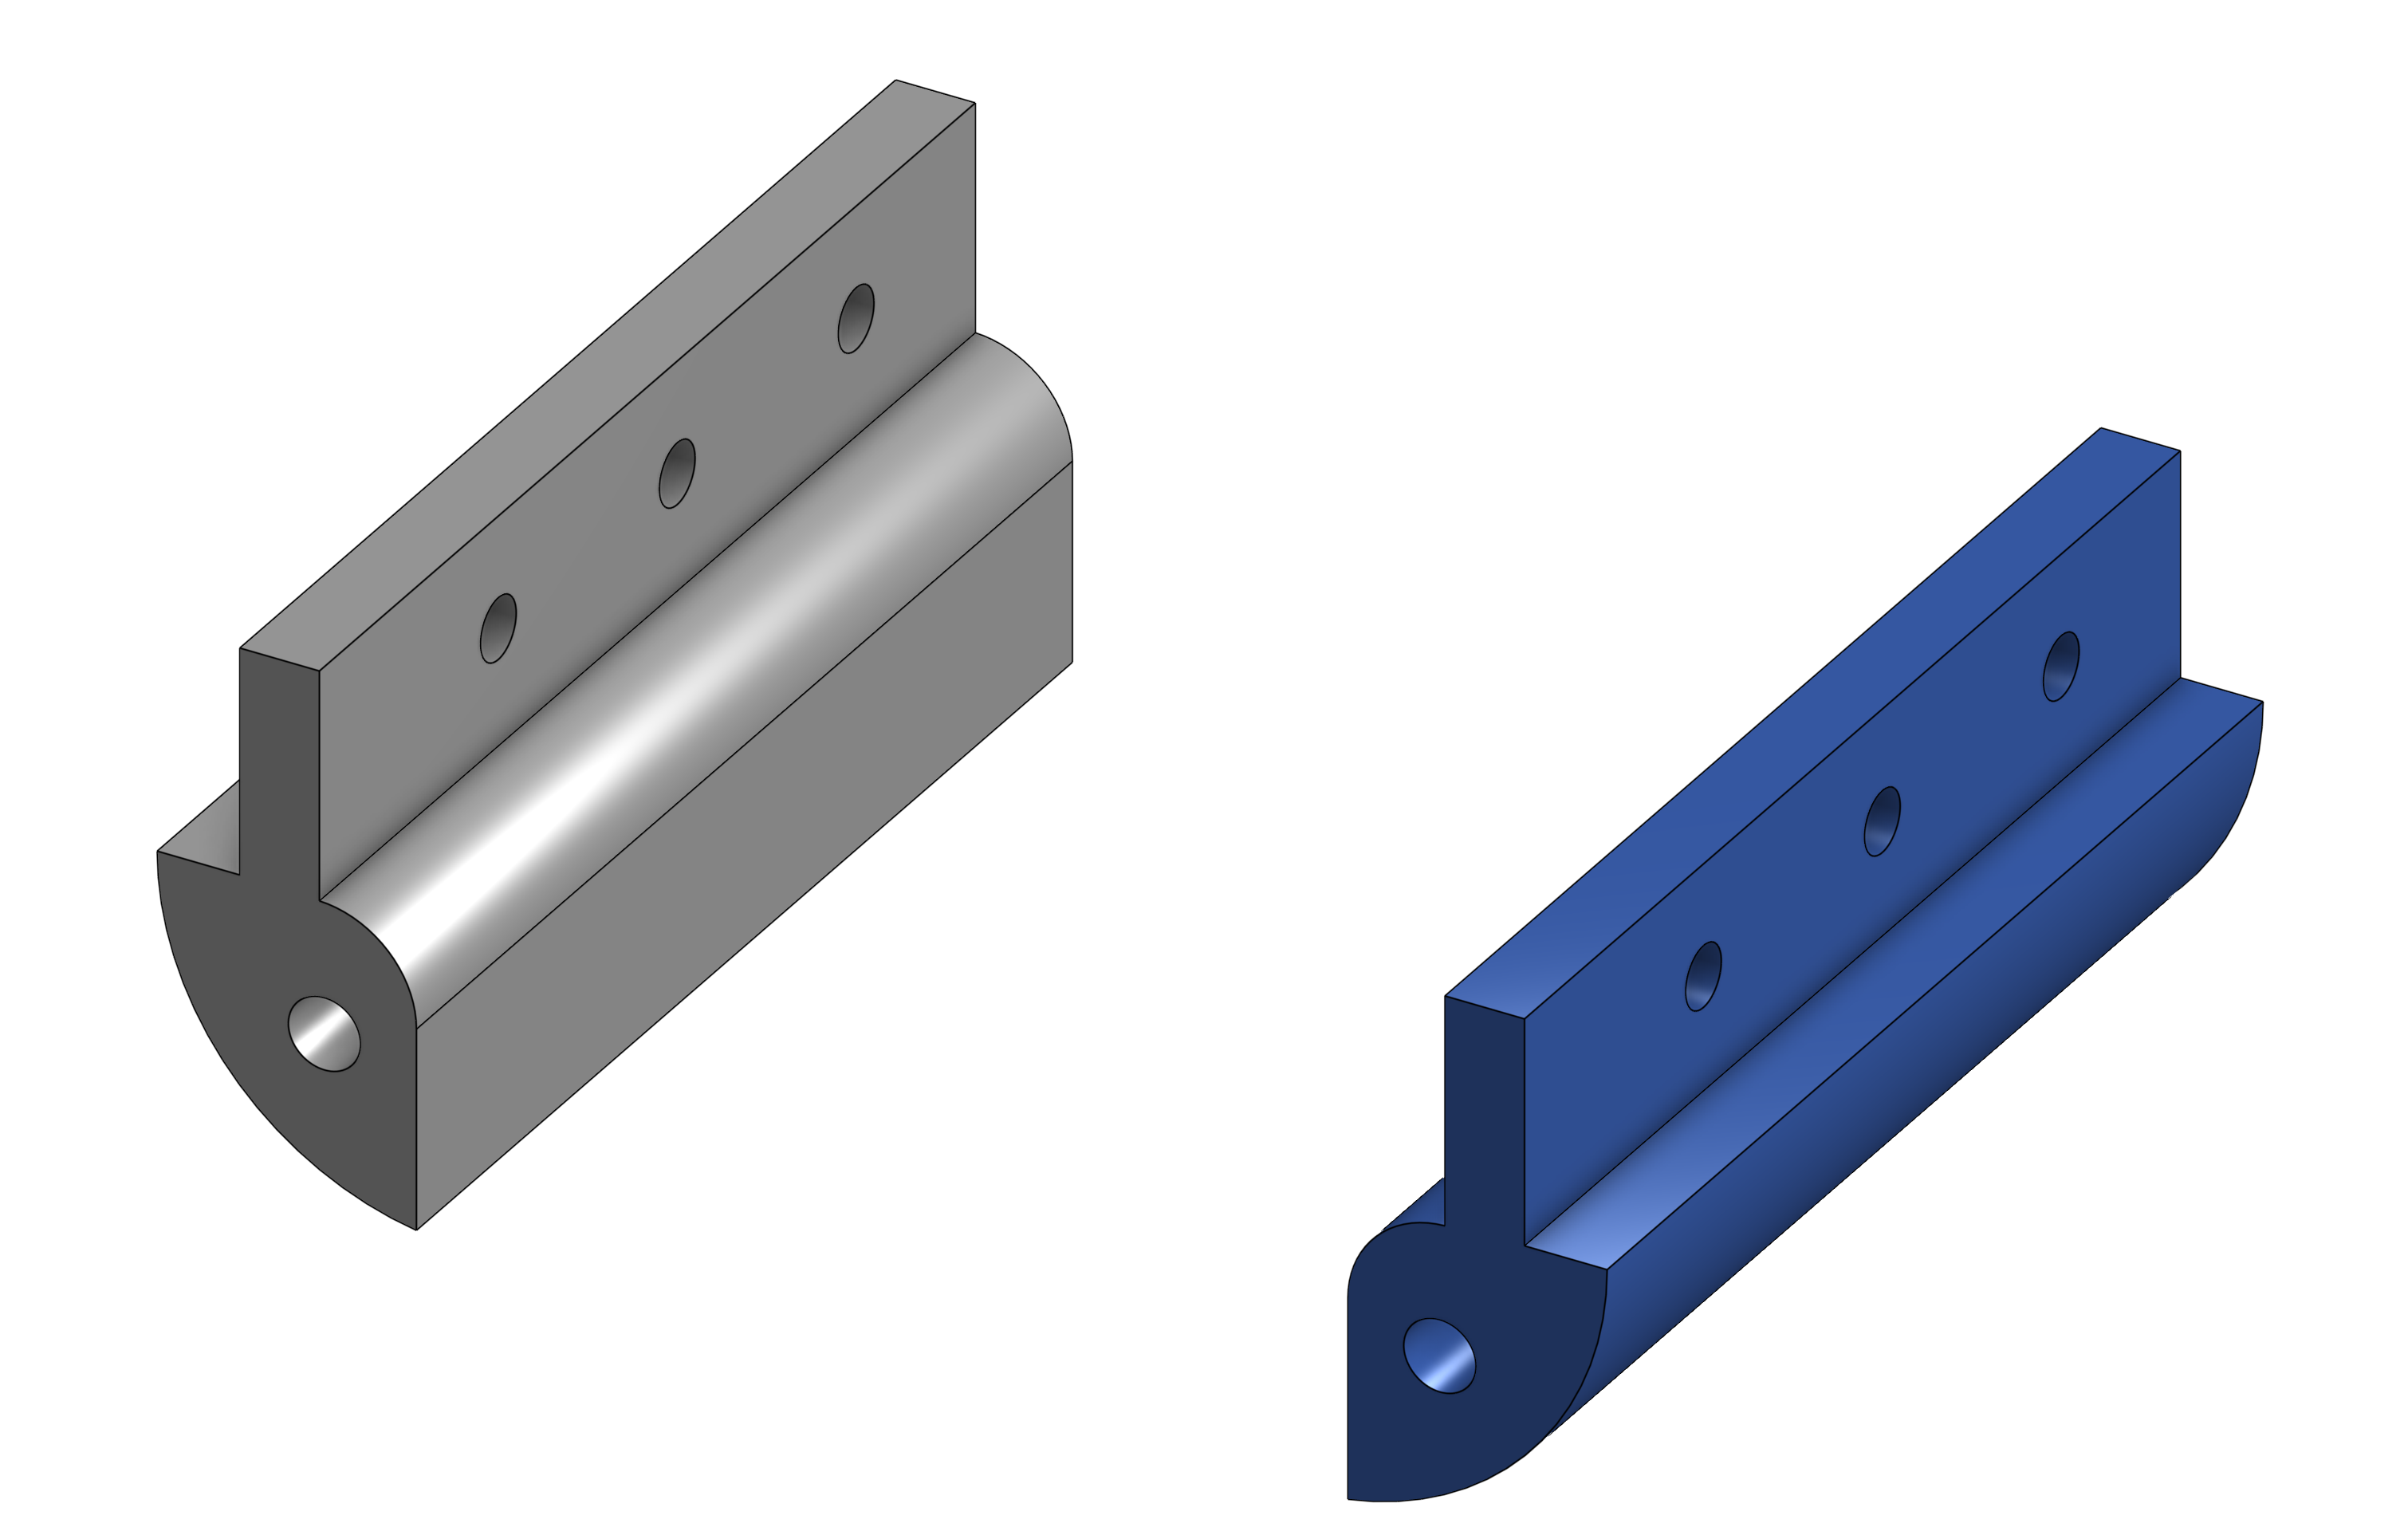
\includegraphics[width=.8\textwidth]{img/bl_br_br.png}
    \caption{The Bottom Left and Right Brace.}
    \label{fig:C_C_Bot} 
\end{figure}

\subsubsection*{Rear Bearing Mounts}

\begin{figure}[H]
    \centering
    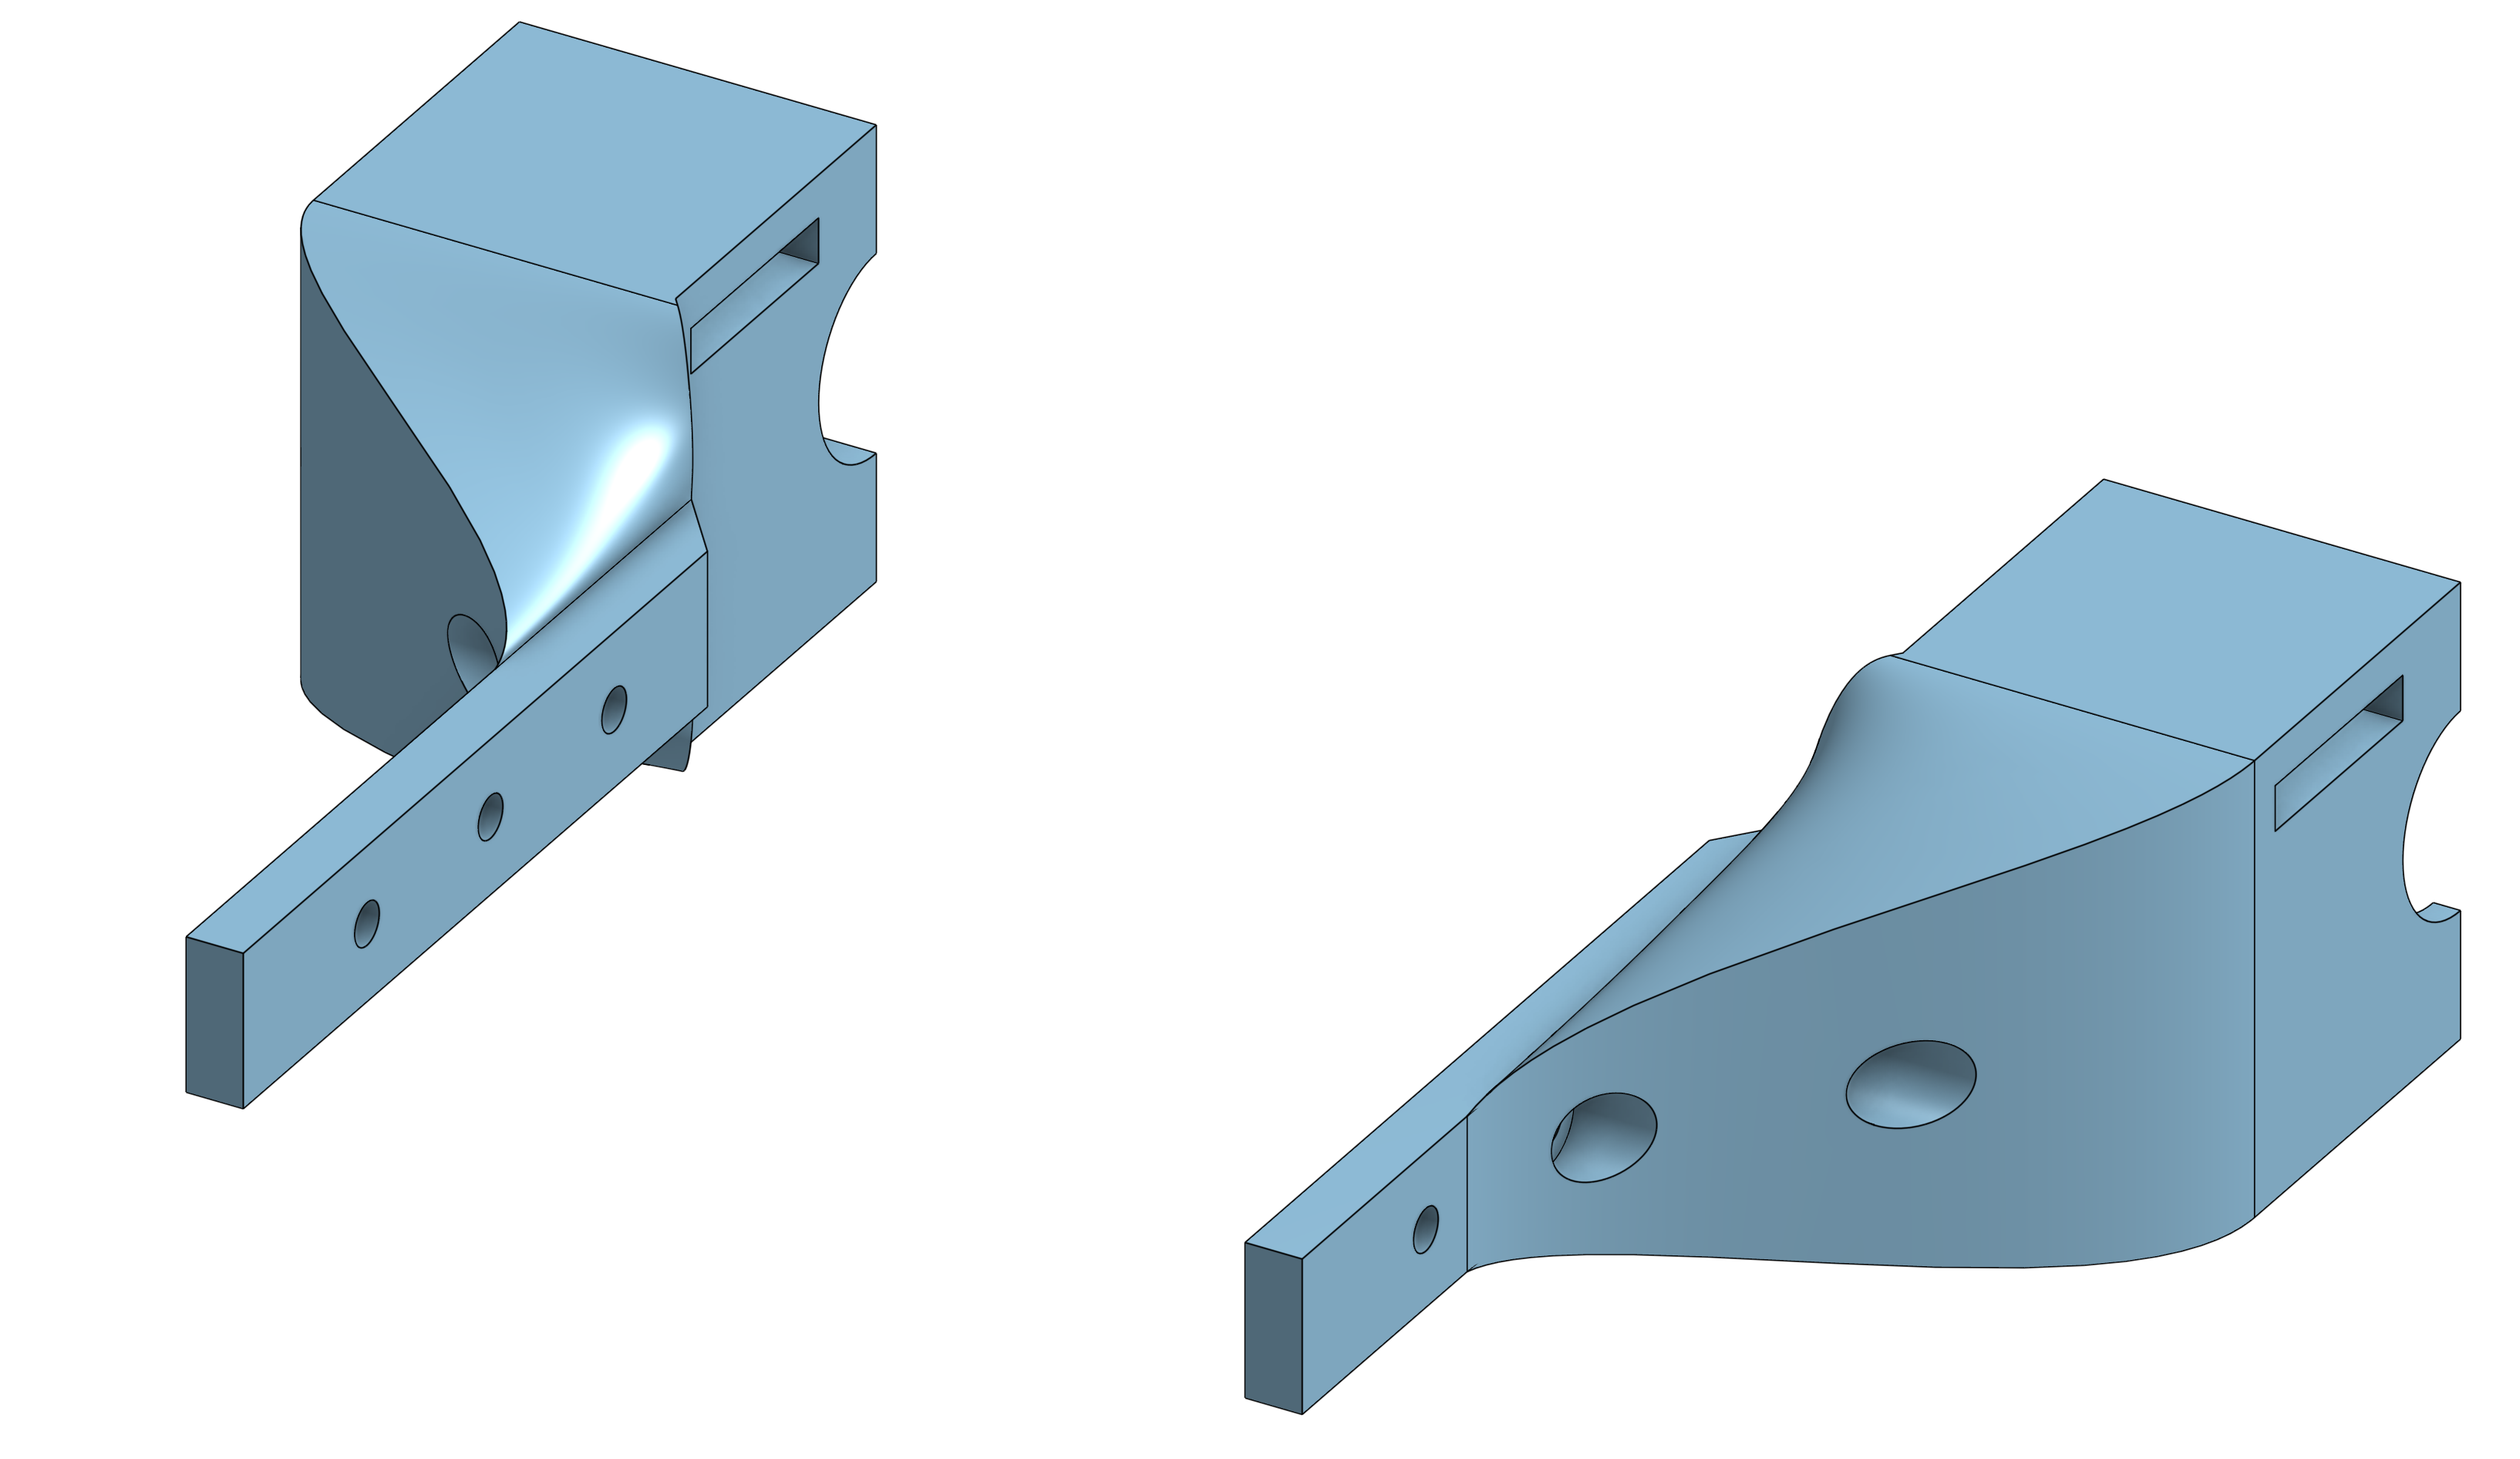
\includegraphics[width=.8\textwidth]{img/rear_bearing_mount.png}
    \caption{The Left and Right Bearing mounts.}
    \label{fig:C_C_Back} 
\end{figure}

These parts go on the outside of the motor mount and top brace sandwich. They serve 2 purposes, one of them is holding the BCWN-T-d12-IR bearing and the other is holding the batteries. The battery straps go though this part. Each one of them is more or less a mirror but the right one has a larger loft for no apparent reason. \\

They are printed with the bottom side facing down. They do not need supports and are printed at a layer height of $0.20$mm, has $3$ perimeters and a $25\%$ infill. A brim is used to aid with bed adhesion and prevent the part from peeling off when printing.

\subsubsection*{LiDAR \& ESC mount}

The LiDAR and ESC mount is one of the two largest parts on the entire vehicle. They mount spans almost the entire breadth of the vehicle. It mouns the ESC on one side, screws into the top brace, mounts the LiDAR and connects to one of the bottom screw holes of the Raspberry Pi. \\

The part has holes to reduce its weight and a recess in on the top to accommodate for the LiDAR's electronics. The ESC has its fan removed and the screws from the shroud are used to mount. There are $3$ M$3 \times 6$mm heat set inserts to mount the LiDAR. The LiDAR uses $3$ M$3 \times 10$ countersunk screws. The mount prints on the face where the ESC mounts from. The part doesn't not need supports, but they are appreciated. It is printed at a layer height of $0.20$mm, has $3$ perimeters and a $25\%$ infill. A brim is used to aid with bed adhesion and prevent the part from peeling off when printing.

\begin{figure}[H]
   \centering
   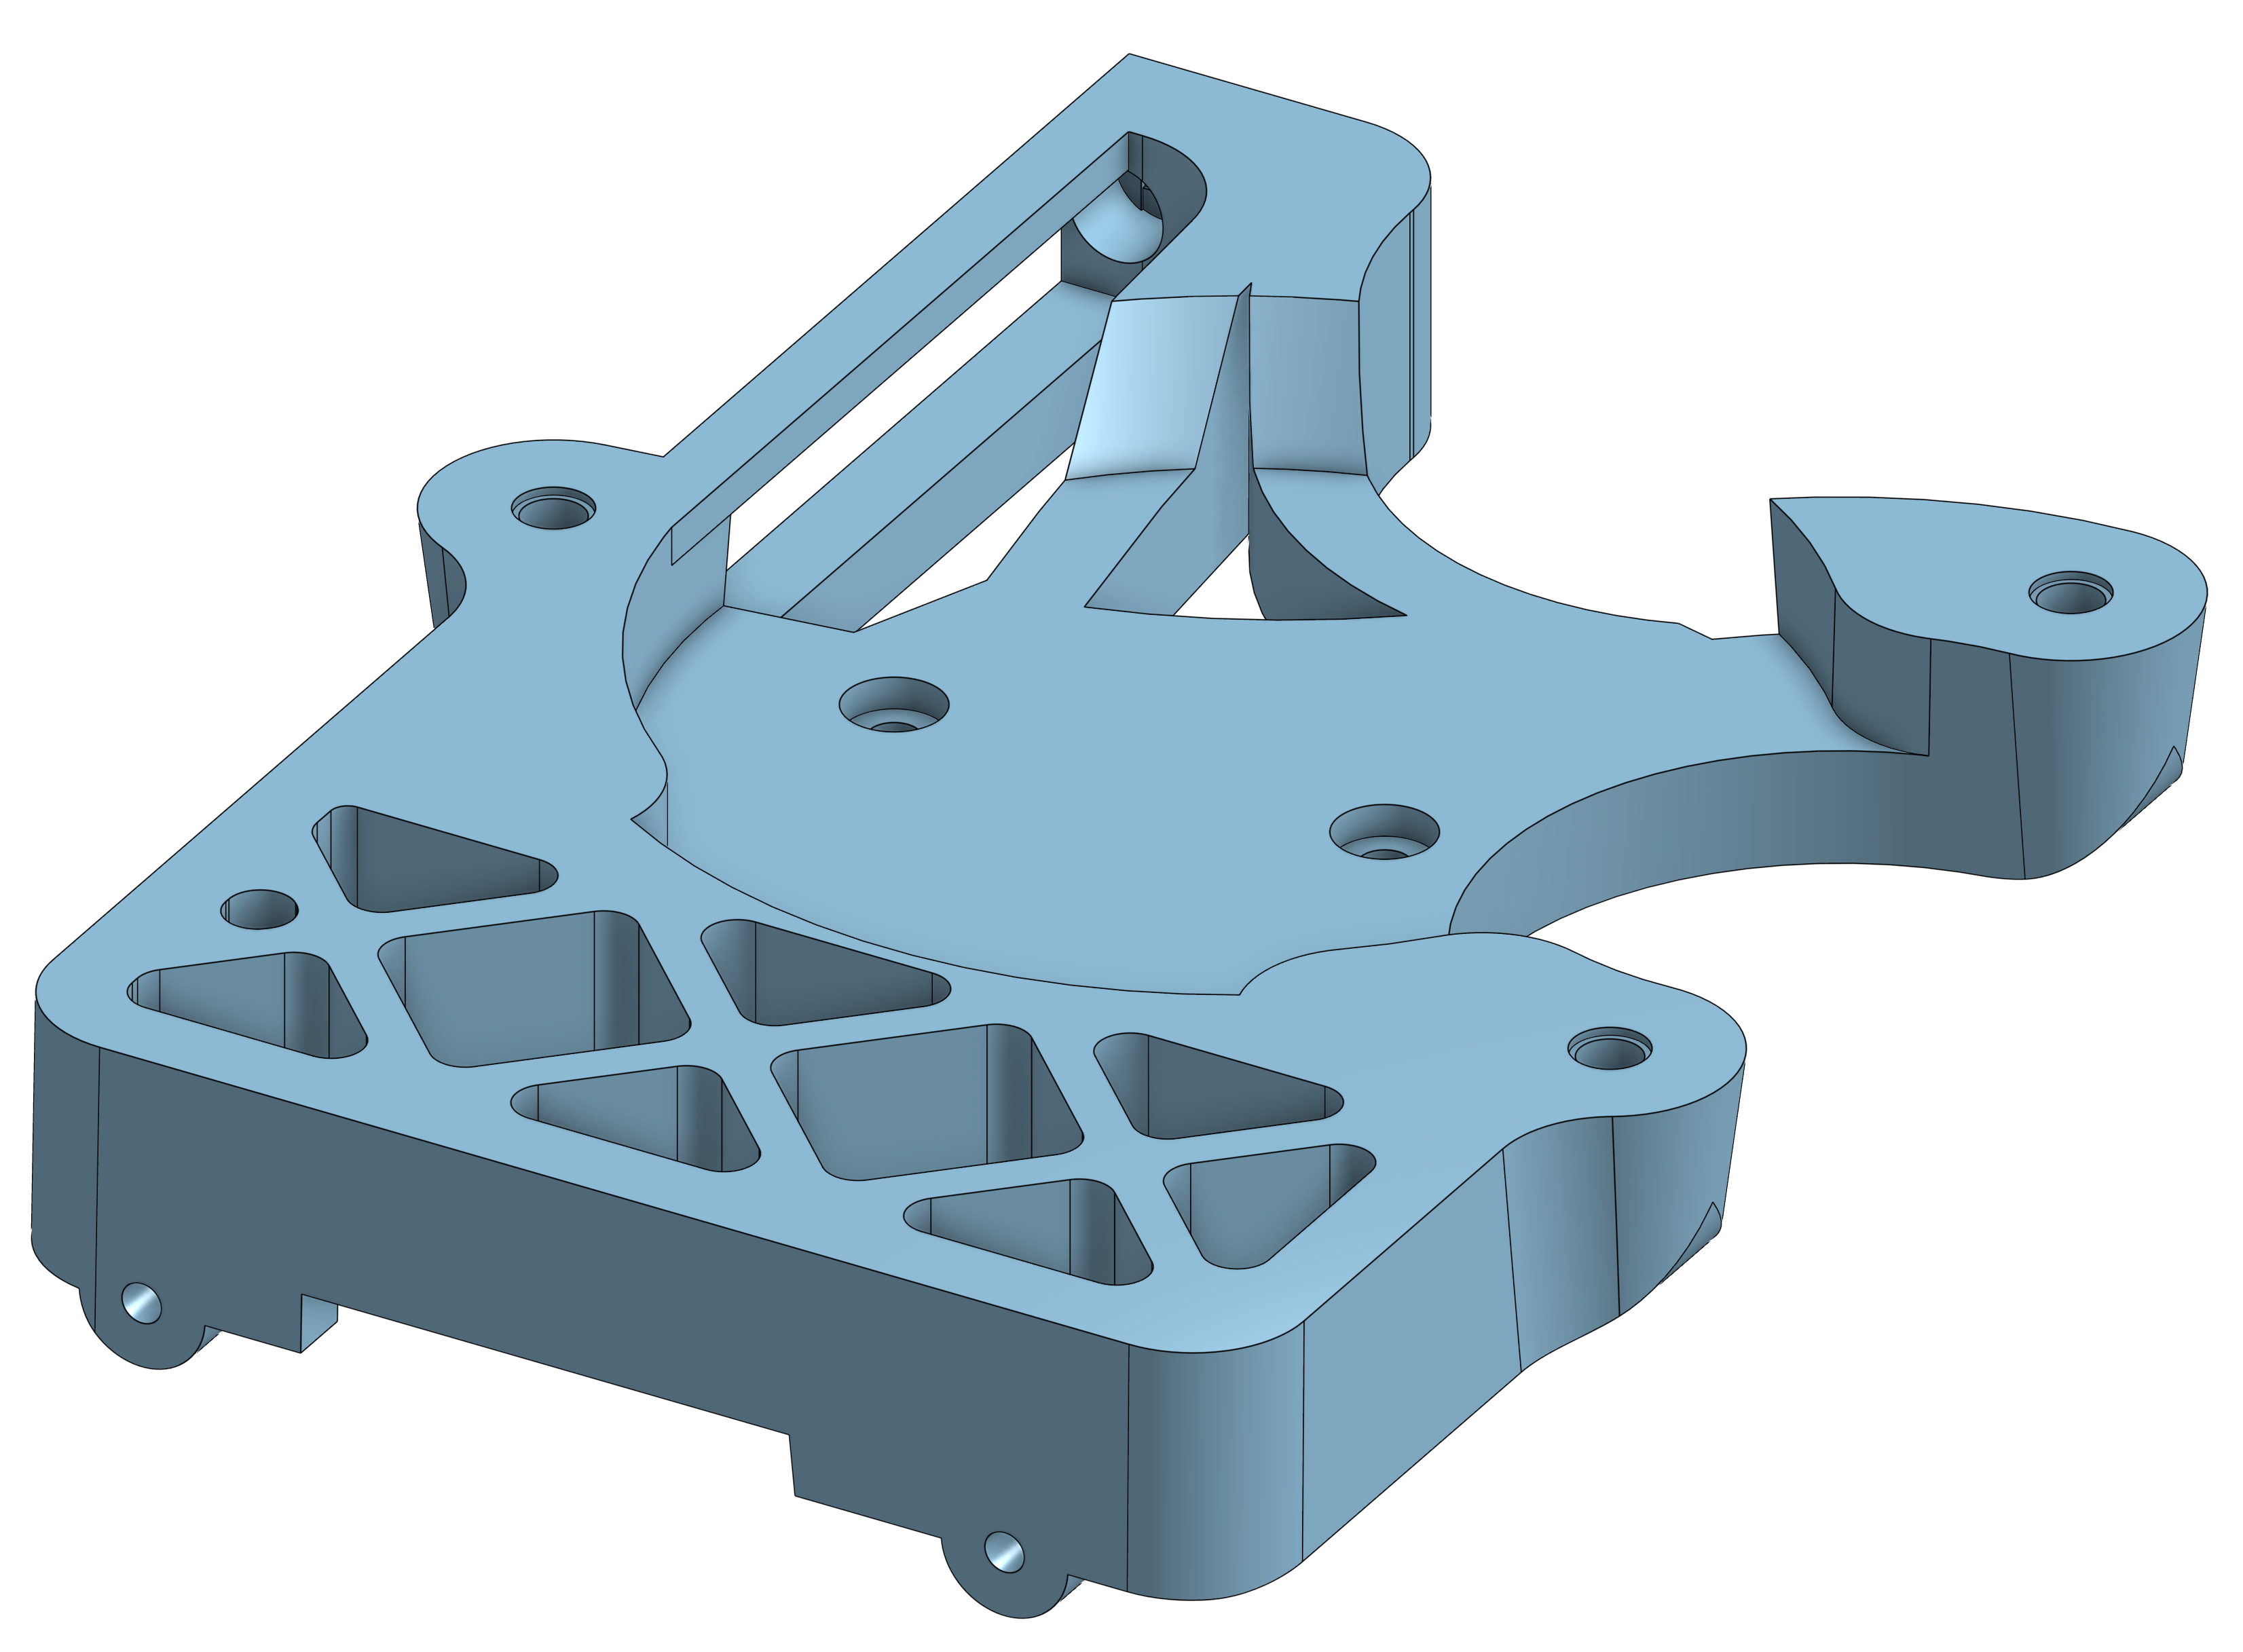
\includegraphics[width=.8\textwidth]{img/lidar_mount.png}
   \caption{The Lidar \& ESC mount.}
   \label{fig:C_C_LM} 
\end{figure}

\subsection{Accessories}

There are several parts that don't fall into a single category but are essential or quality of life improvements.

\subsubsection*{Wheel Hub}
\label{Wheel Hub}
The wheel hub is the part that goes around the custom silicone casting as discussed earlier. It has to grip the cast tire and attach to the axles securely. To do this, it uses a single M$2 \times 12$mm screw. The wheel hub is  a tight interference fit with both the wheel and the axle. It is $18$mm wide, same as the cast tire. \\

The wheel hub is printed at a layer height of $0.20$mm has $3$ perimeters and a $25\%$ infill. A brim is used to aid with bed adhesion and prevent the part from peeling off when printing. The outer surface (where the wheel hub and tire touch), see Figure \ref{fig:C_W_H}, has a fuzzy skin, with a thickness of $0.1$mm and $0.2$mm. \\

\begin{figure}[H]
   \centering
   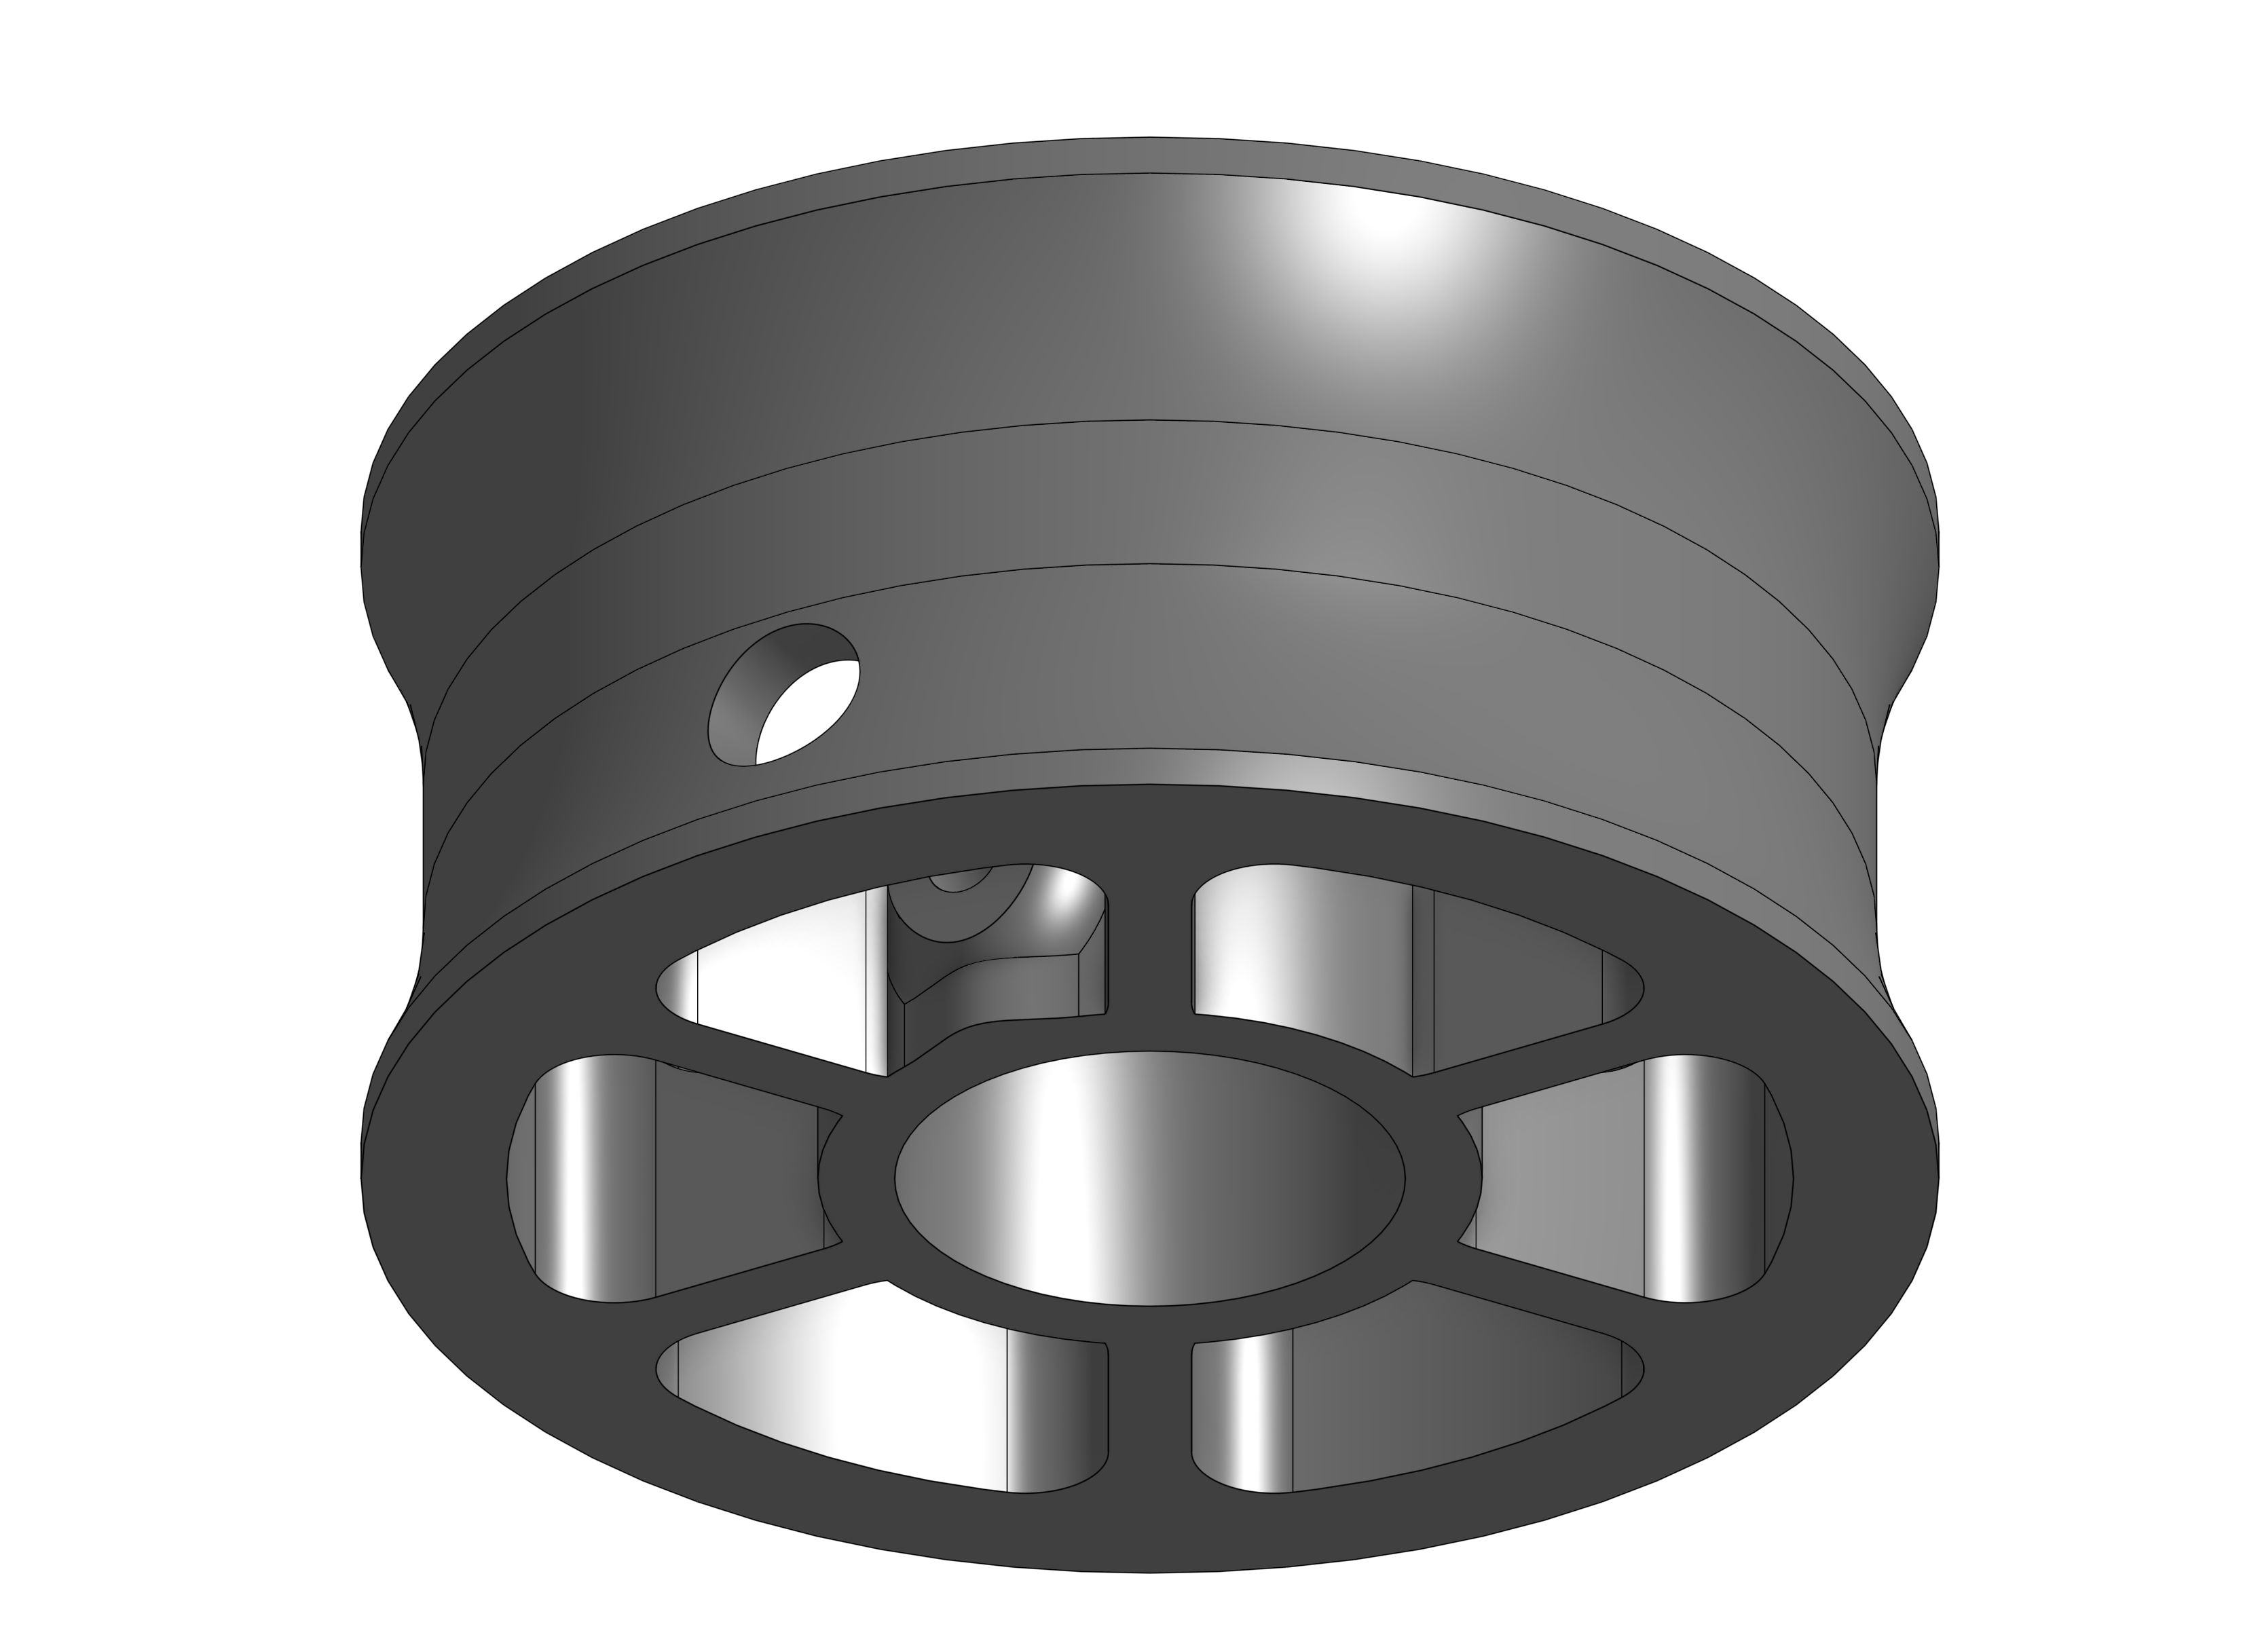
\includegraphics[width=.8\textwidth]{img/wheel_hub.png}
   \caption{The Wheel Hub.}
   \label{fig:C_W_H} 
\end{figure}

\subsubsection*{Raspberry Pi Mount}

This part holds the raspberry pi by the forward $2$ mounting holes and constrains it via attaching it to the bottom $2$ carbon fiber brace rods. The part is fairly simple. It interfaces with the $\diameter 3$mm rods via holes and interfaces with the pi with $2$ M$2.5 \times 8$mm screws. \\

The part is printed with any of the large, flat faces (see Figure \ref{fig:C_A_RPM}) facing down and does not need supports. It is printed at a layer height of $0.20$mm, has $3$ perimeters and a $25\%$ infill. \\

\begin{figure}[H]
   \centering
   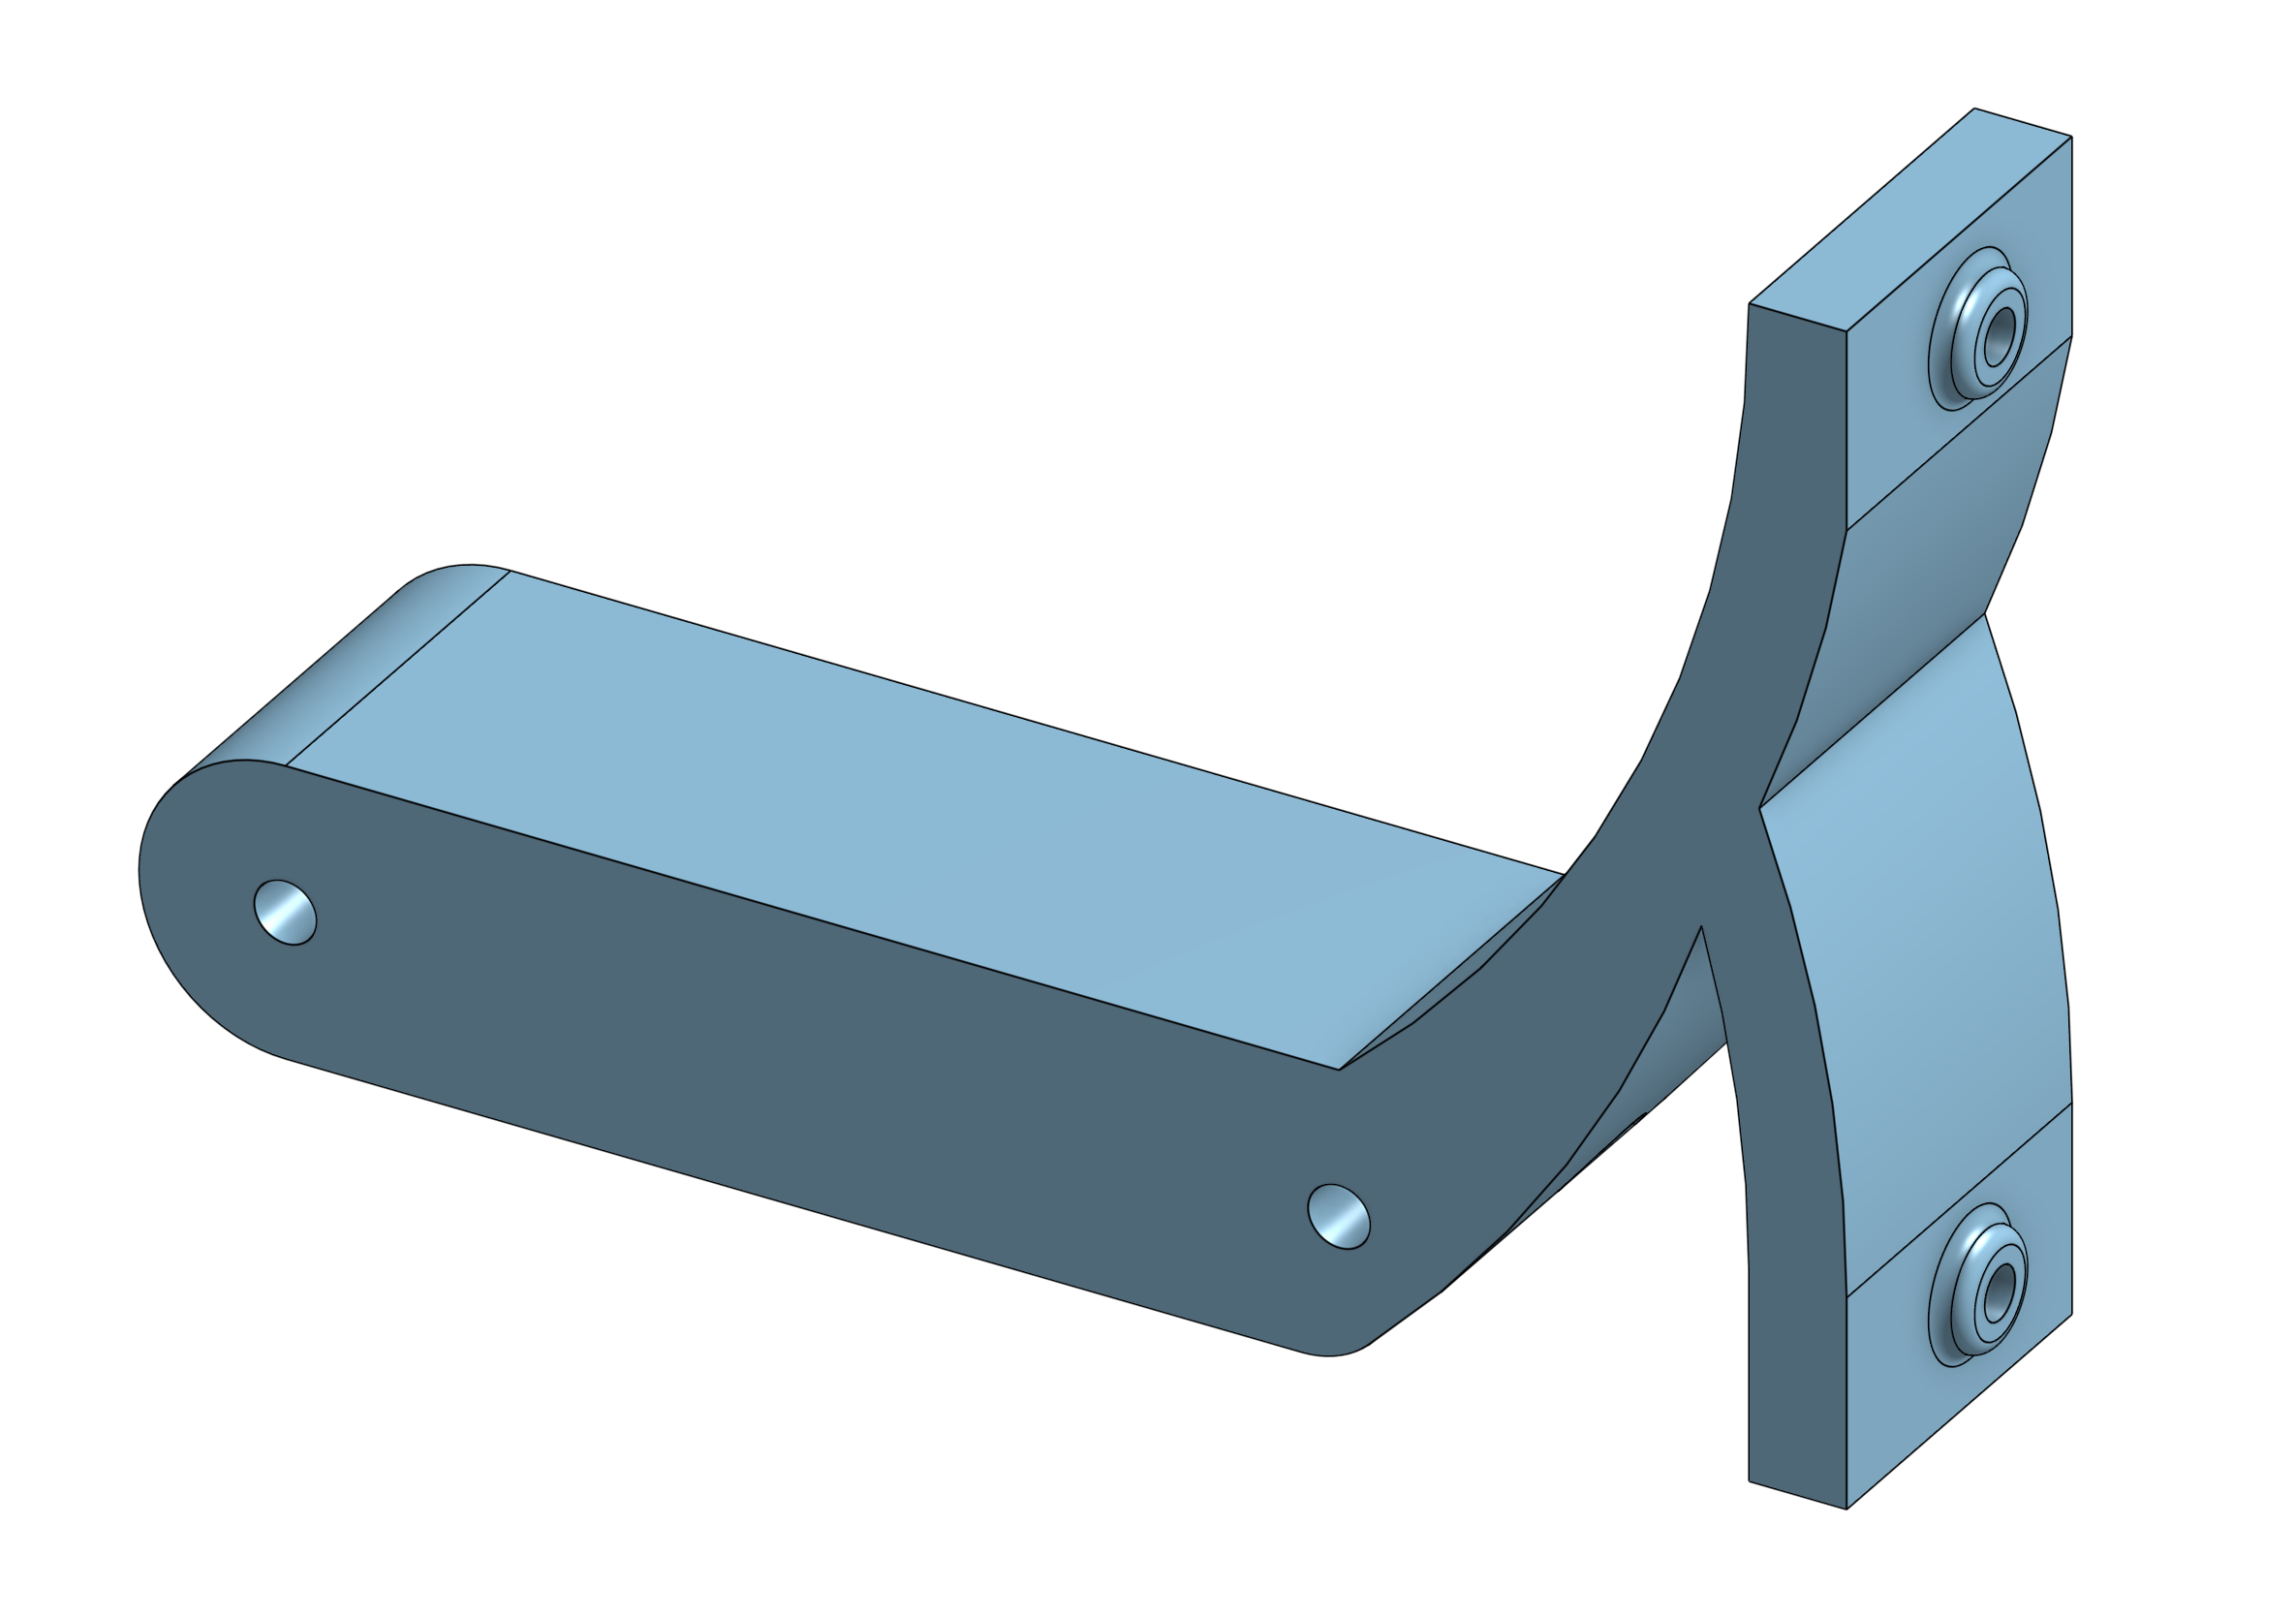
\includegraphics[width=.8\textwidth]{img/rpi_mount.png}
   \caption{The Raspberry Pi Mount.}
   \label{fig:C_A_RPM} 
\end{figure}

\subsubsection*{ESC Wire Mount}

This is a very simple part that attaches with the bottom right brace rod and uses zip-ties to helpd the motor and ESC wires in a neat bundle. It's only $2$mm think and serves the purpose. The part is printed with any of the large, flat faces (see Figure \ref{fig:C_A_Wmount}) facing down and does not need supports. It is printed at a layer height of $0.20$mm, has $3$ perimeters and a $25\%$ infill.

\begin{figure}[H]
   \centering
   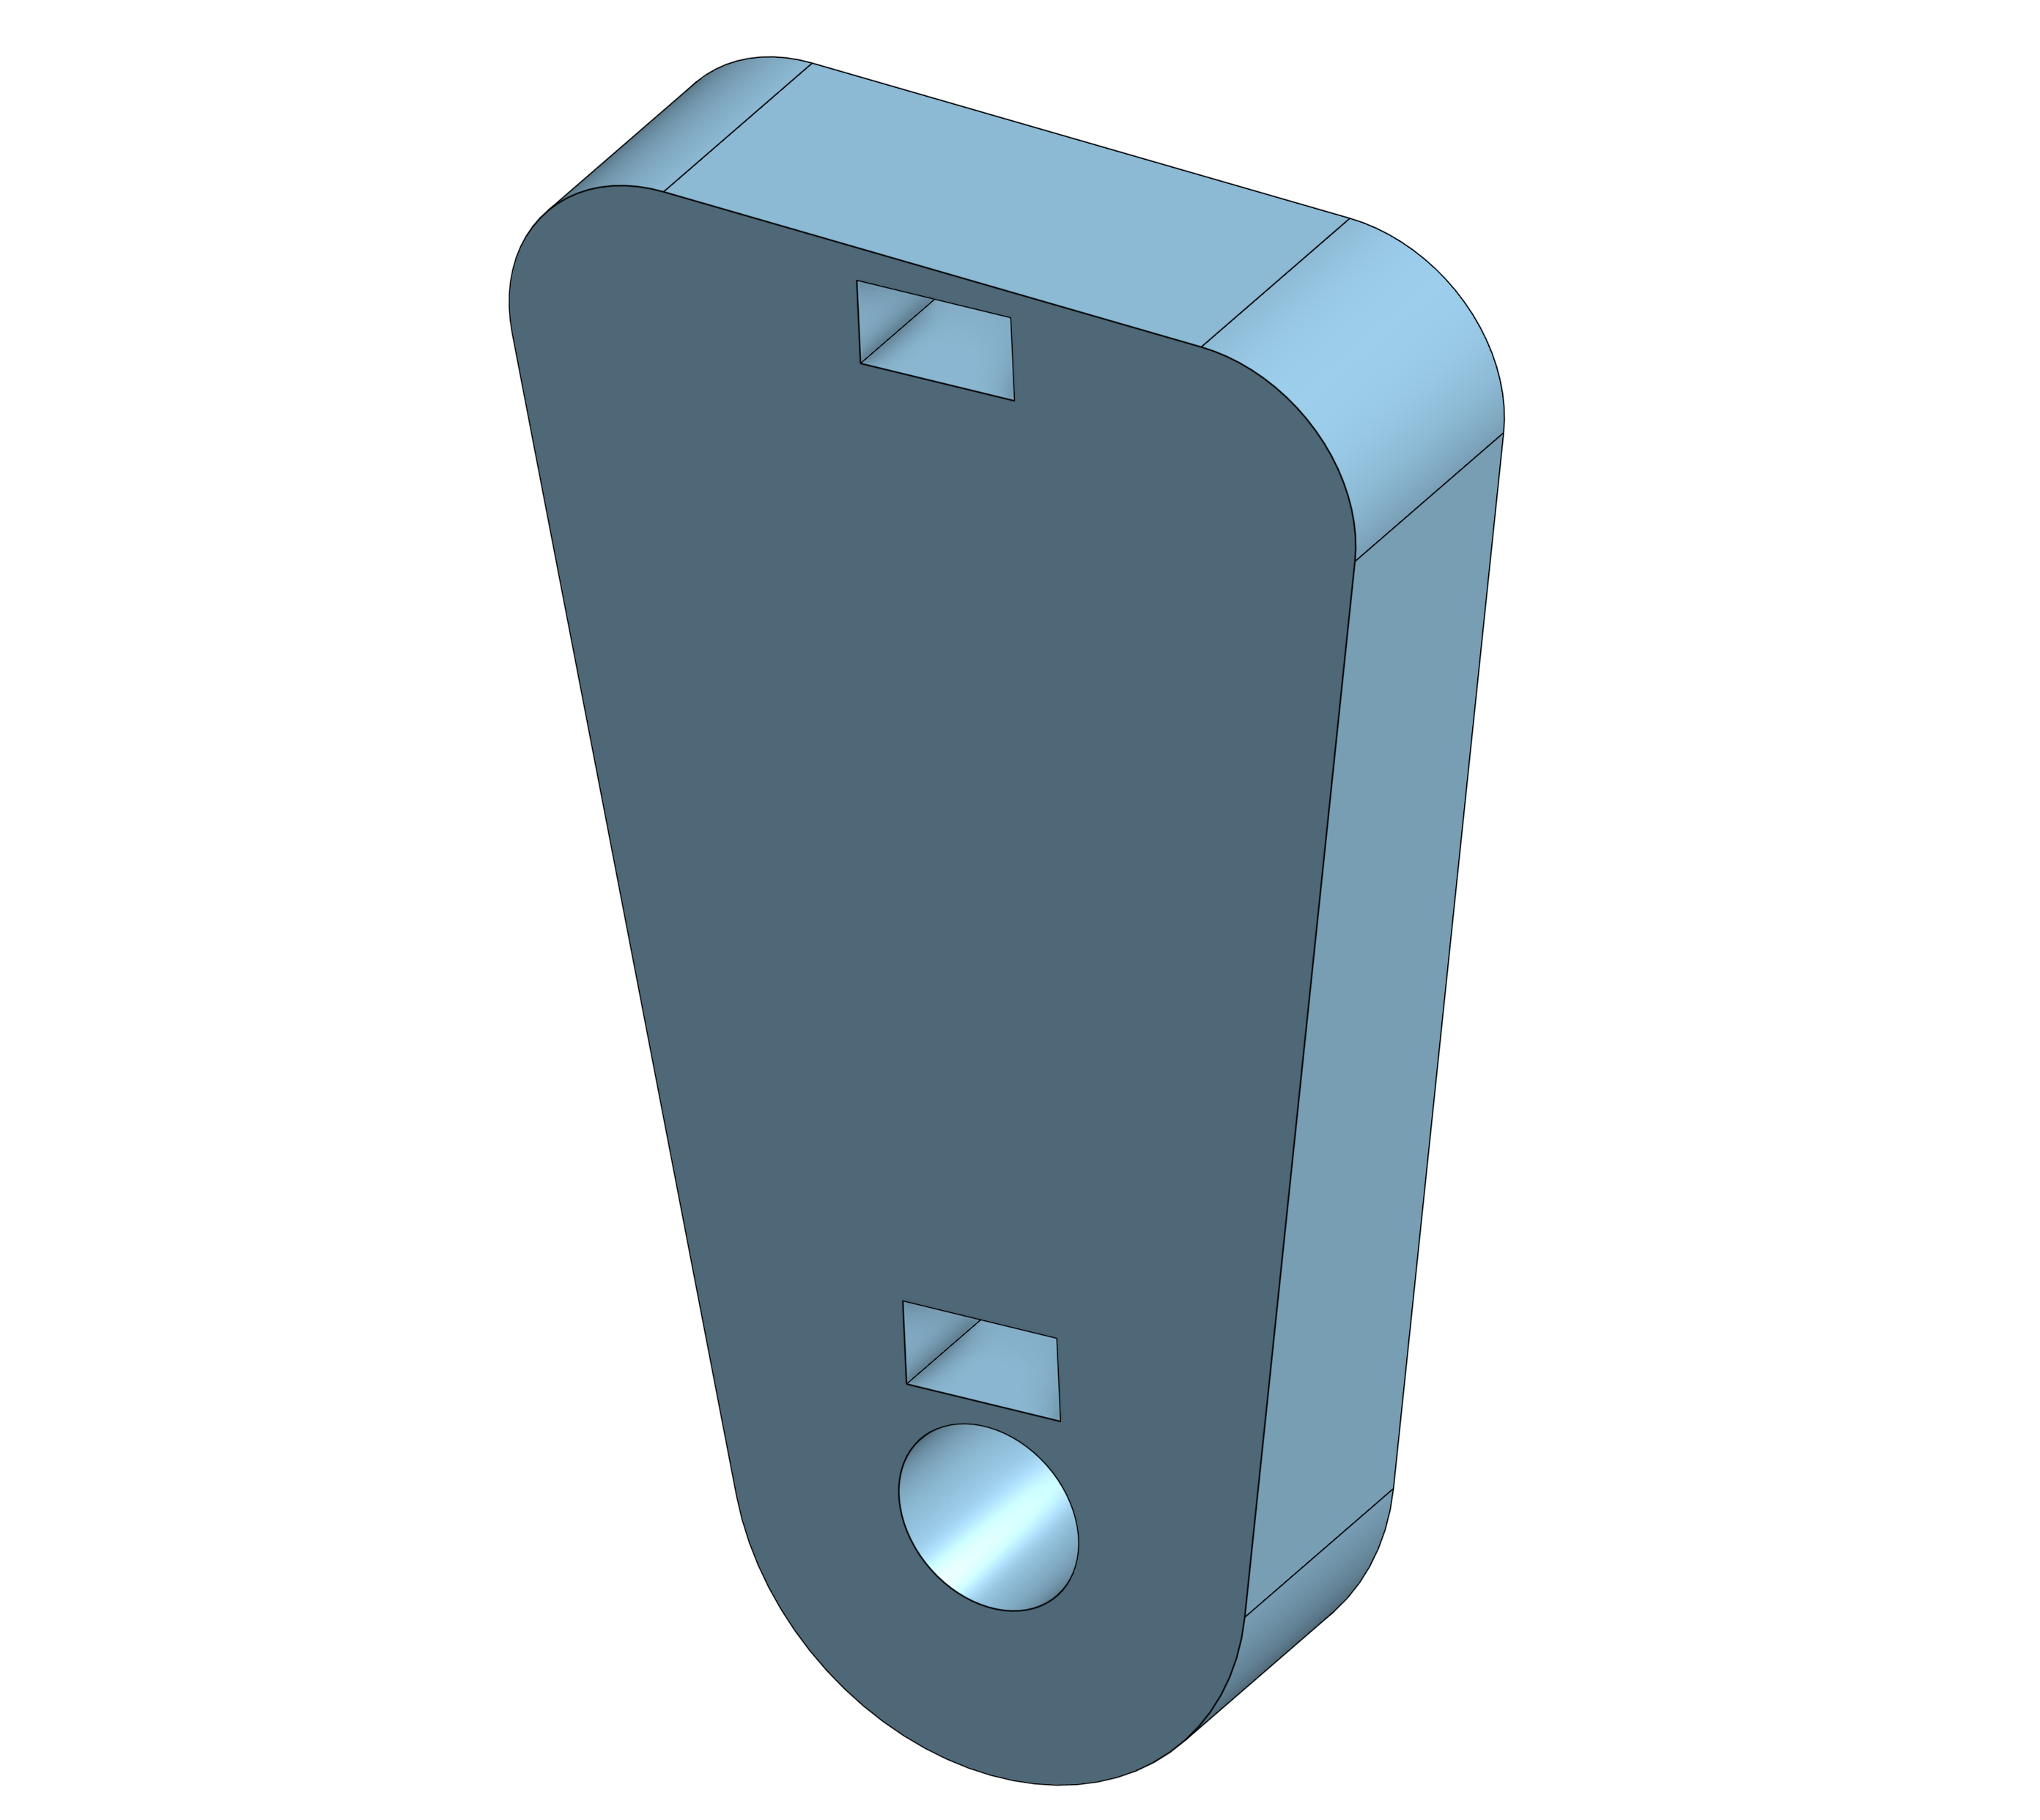
\includegraphics[width=.6\textwidth]{img/esc_wire_mount.png}
   \caption{The ESC Wire Mount.}
   \label{fig:C_A_Wmount} 
\end{figure}

\subsection{Tools}

There were several tools used for cutting, drilling and casting. These tools don't make it to the final vehicle but are an integral part of the buld process.

\subsubsection*{Tire Molds}

The mold for the tire, as mentioned earlier, is printed in Resin via the SLA manufacturing process. It is a two part mold that clamps via $4$ M$3 \times 30$mm screws and M$3$ nuts. It is advised to add washers to both sides. The mold does not have any draft angles as it was intended to be resin printed where the layer lines are microscopic and can be filled in by mold release. The mold can be FDM printed but would need draft angles. \\

It is a simple $2$ par mold that has the negatives for the tire. The top and bottom are more or less mirrors of each other with the only difference being that the top has an entry and exit hole to help with the pouring process. \\

\begin{figure}[H]
   \centering
   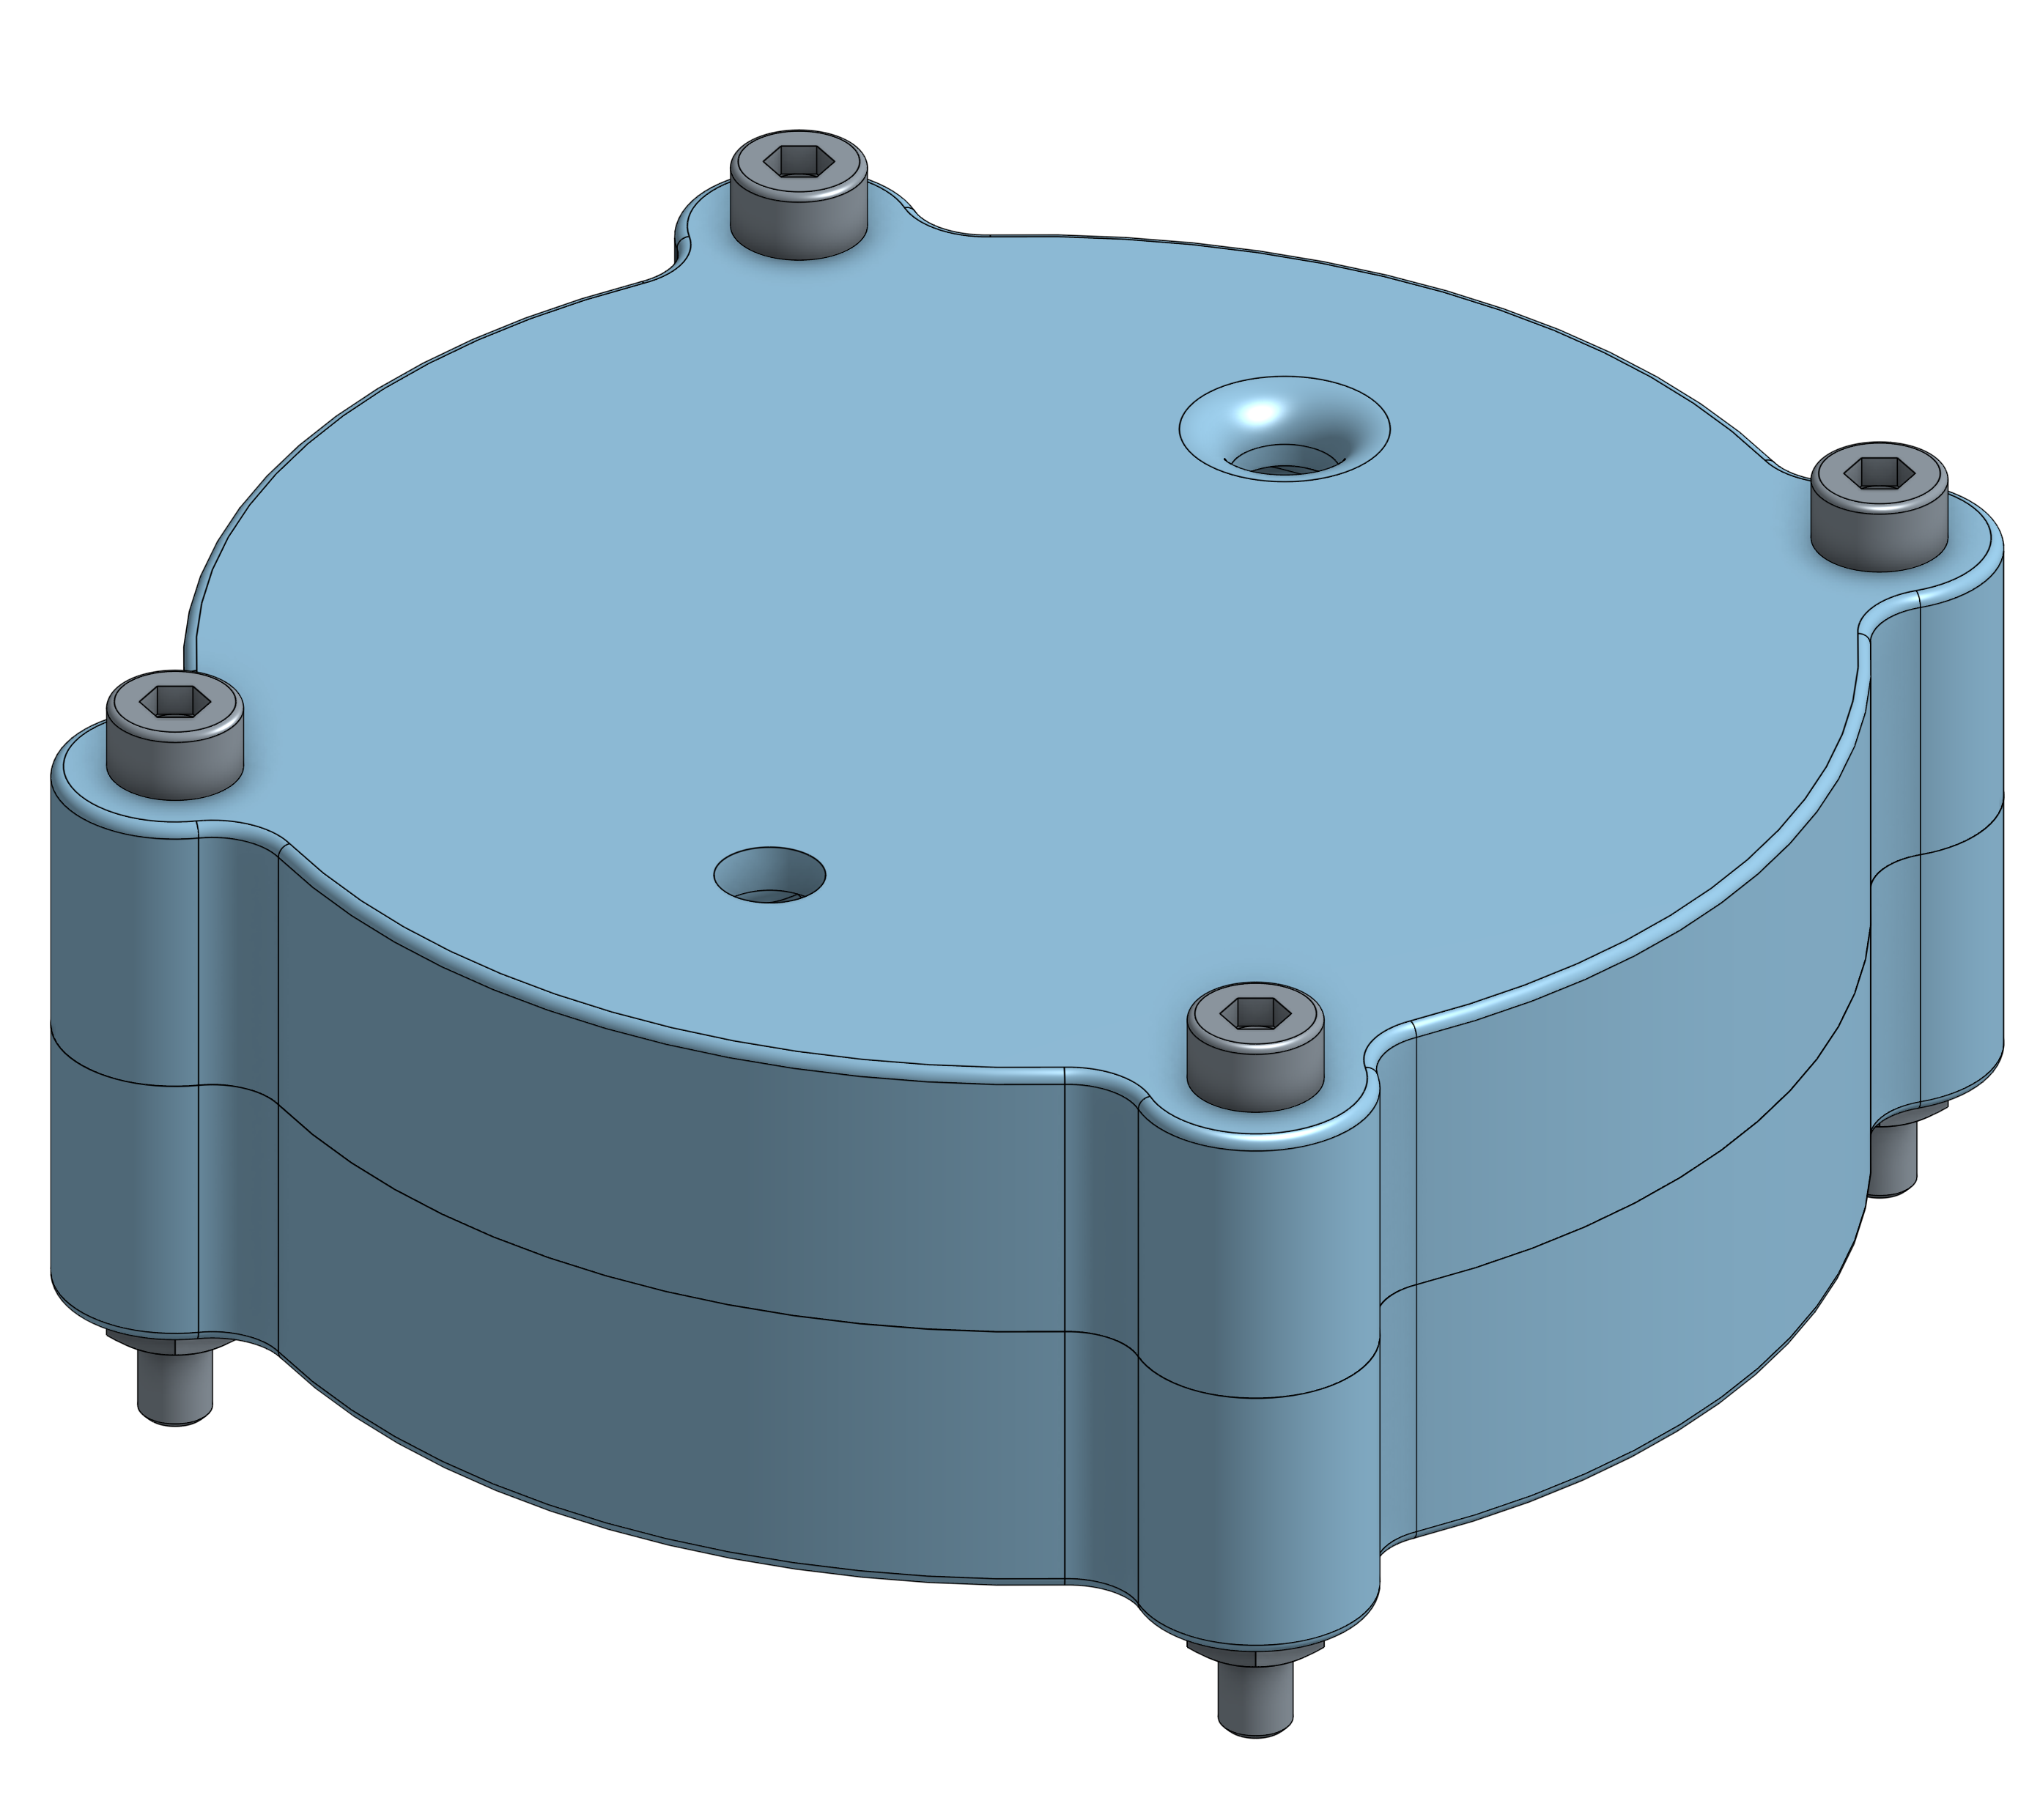
\includegraphics[width=.6\textwidth]{img/tire_mold.png}
   \caption{The Mold for the Polyurethane Tire.}
   \label{fig:C_W_Mold} 
\end{figure}

\subsubsection*{Standoff Cutting}

To attach the Raspberry Pi to the custom hat, $15$mm nylon female to female standoffs are used. However, the actual spacing comes out to be $14$mm. For a better fit, we decided to cut the standoffs to length, \textbf{however, this is completely optional}. To do this, a simple tool was made. \\

The part has the space for the standoff where it is pressed against a wall. It has a slit for a razor blade that allows it to slot in and cut straight and at length. The part is printed upright, as depicted in Figure \ref{fig:C_T_SC}. It is printed at a layer height of $0.20$mm, has $3$ perimeters and a $25\%$ infill.

\begin{figure}[H]
   \centering
   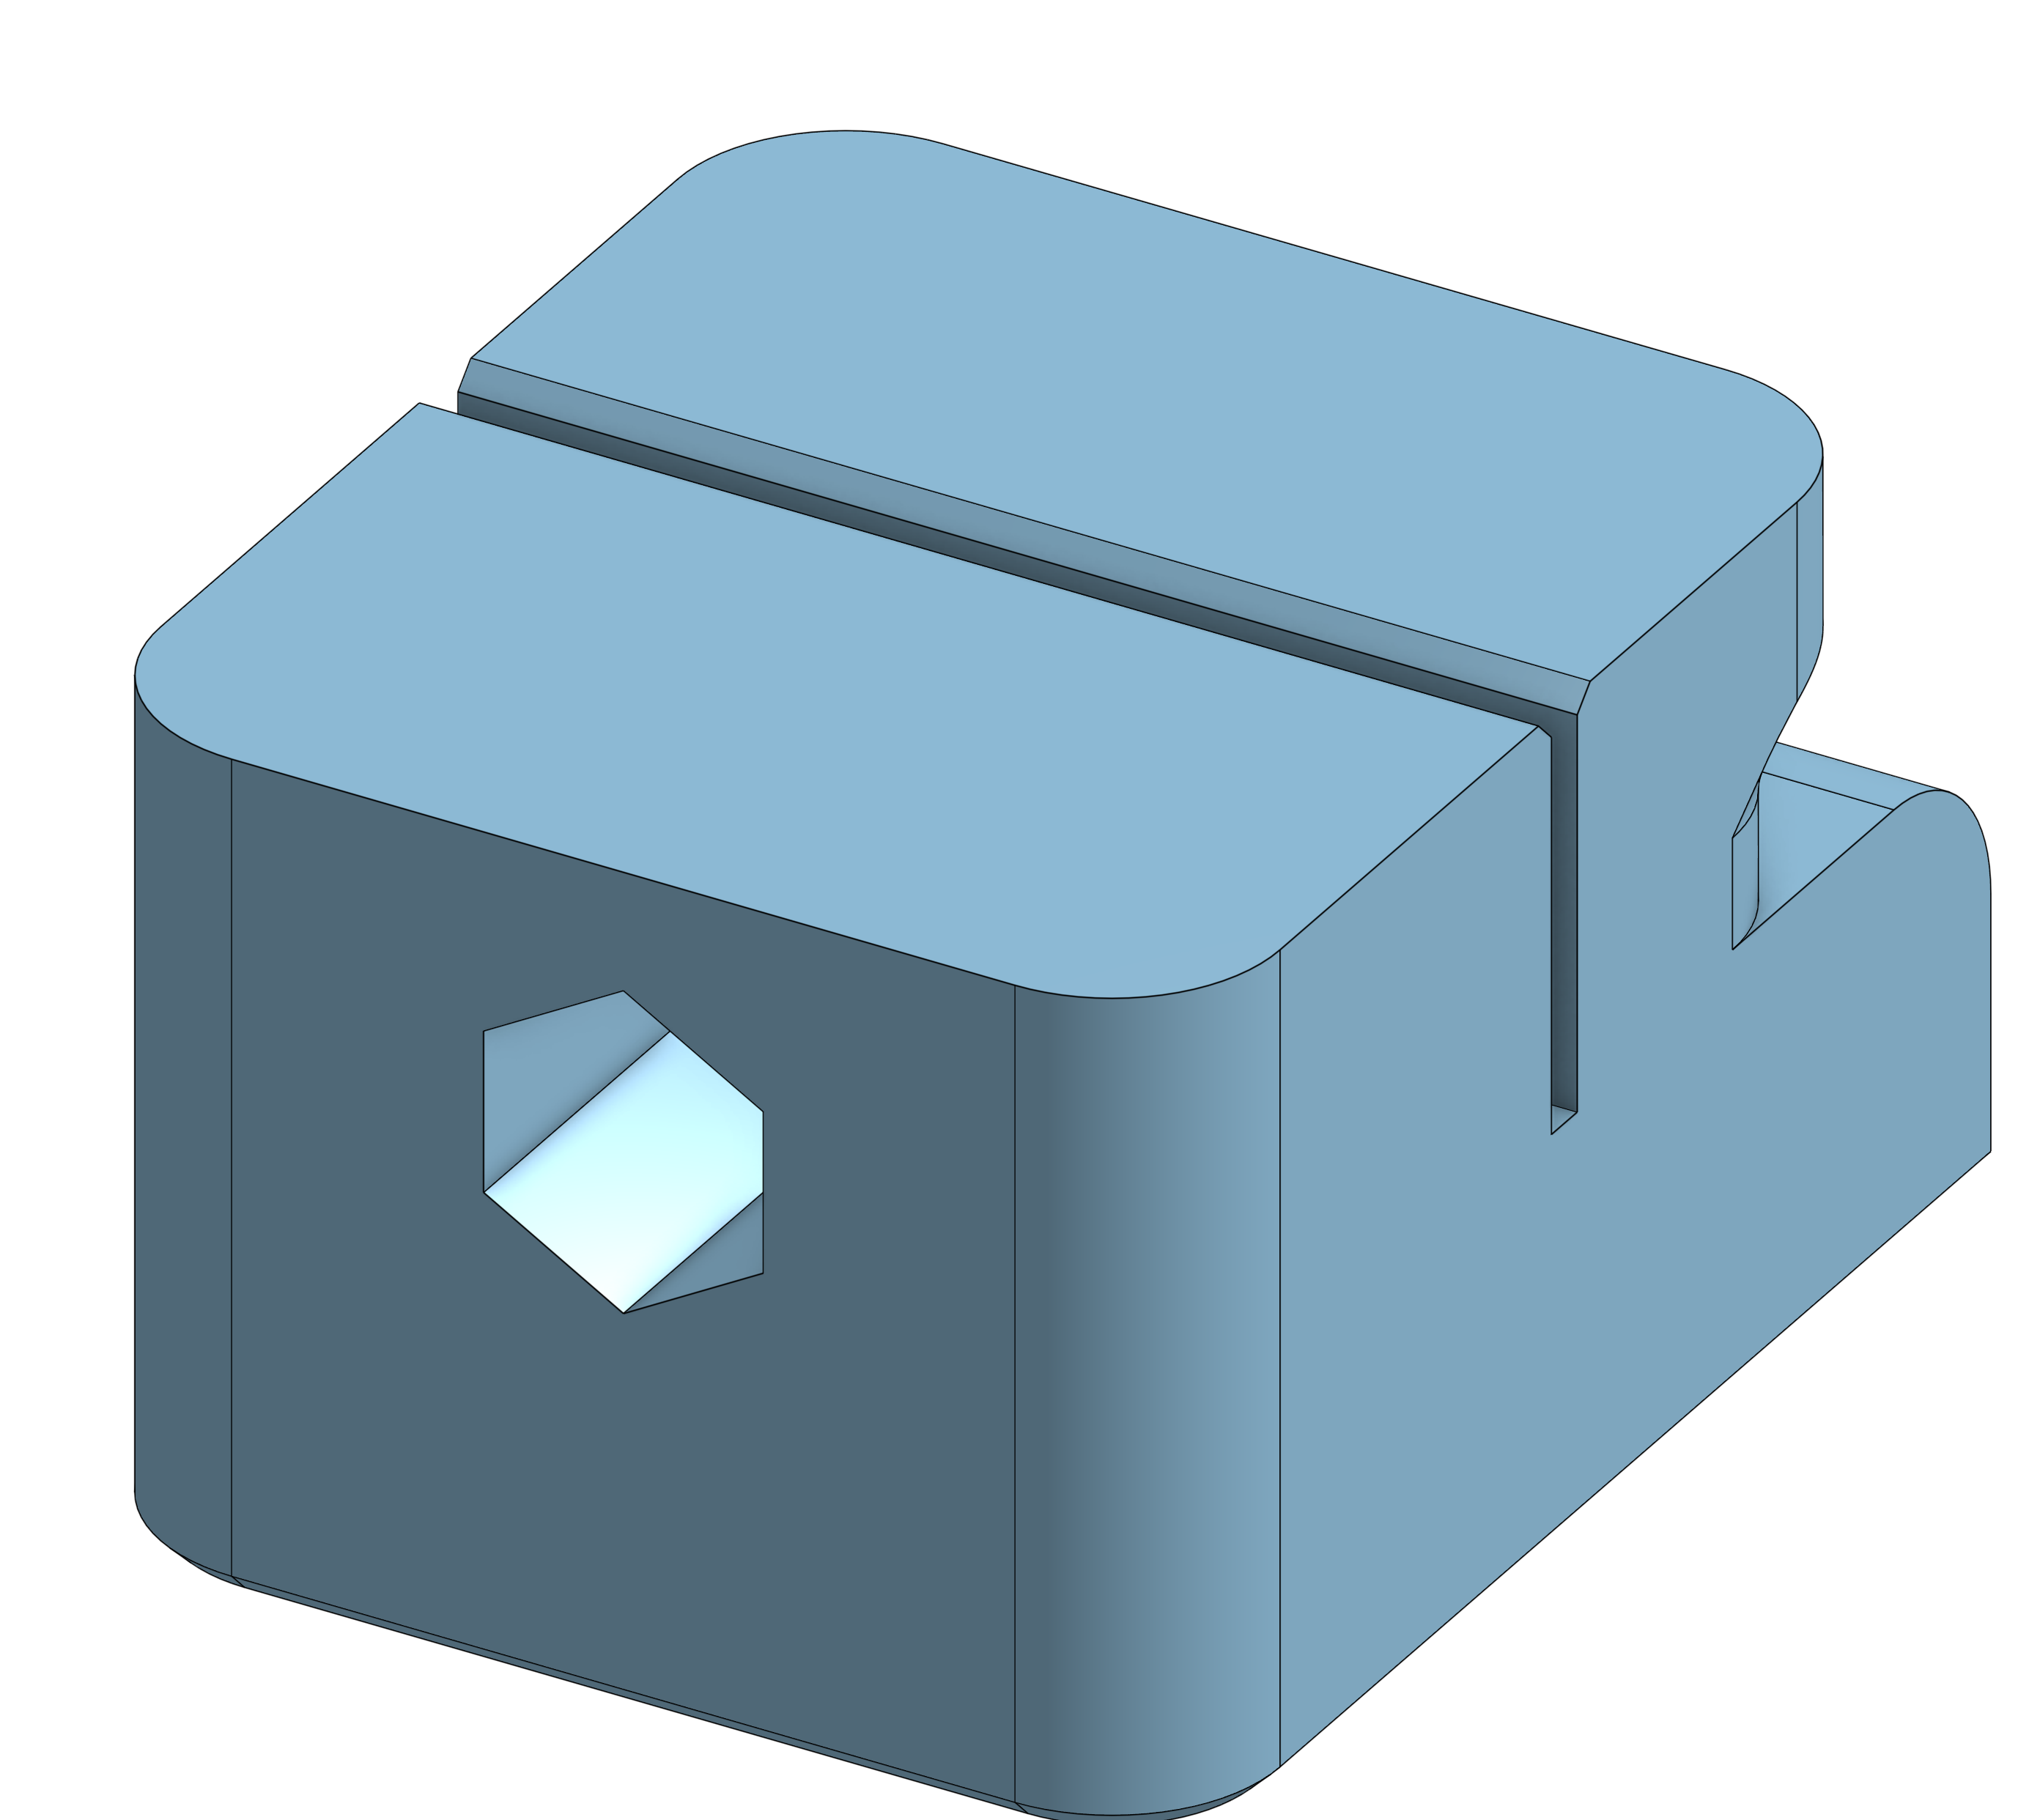
\includegraphics[width=.6\textwidth]{img/standoff_cutting.png}
   \caption{The Standoff Cutting Tool.}
   \label{fig:C_T_SC} 
\end{figure}

\subsubsection*{Axle Cutting}

\textbf{Caution:} \textit{Carbon Fiber dust is not very nice to inhale, all carbon fiber related tasks that involve manufacturing should be done with the part submerged in water to prevent the dust getting in the air and in a well ventilated area with a respirator and eye protection.} \\

The rear axle consists of $2$ $\diameter 12 \times 60$mm Carbon fiber tubes. The tube sourced was $500$mm in length. To cut it down to length, a tool was needed. \\

The part takes in the carbon fiber tube until it is pressed against an inner wall. It has a slit for the saw blade. It is printed upright, as depicted in Figure \ref{fig:C_T_RC}. It is printed at a layer height of $0.20$mm, has $3$ perimeters and a $25\%$ infill.

\begin{figure}[H]
   \centering
   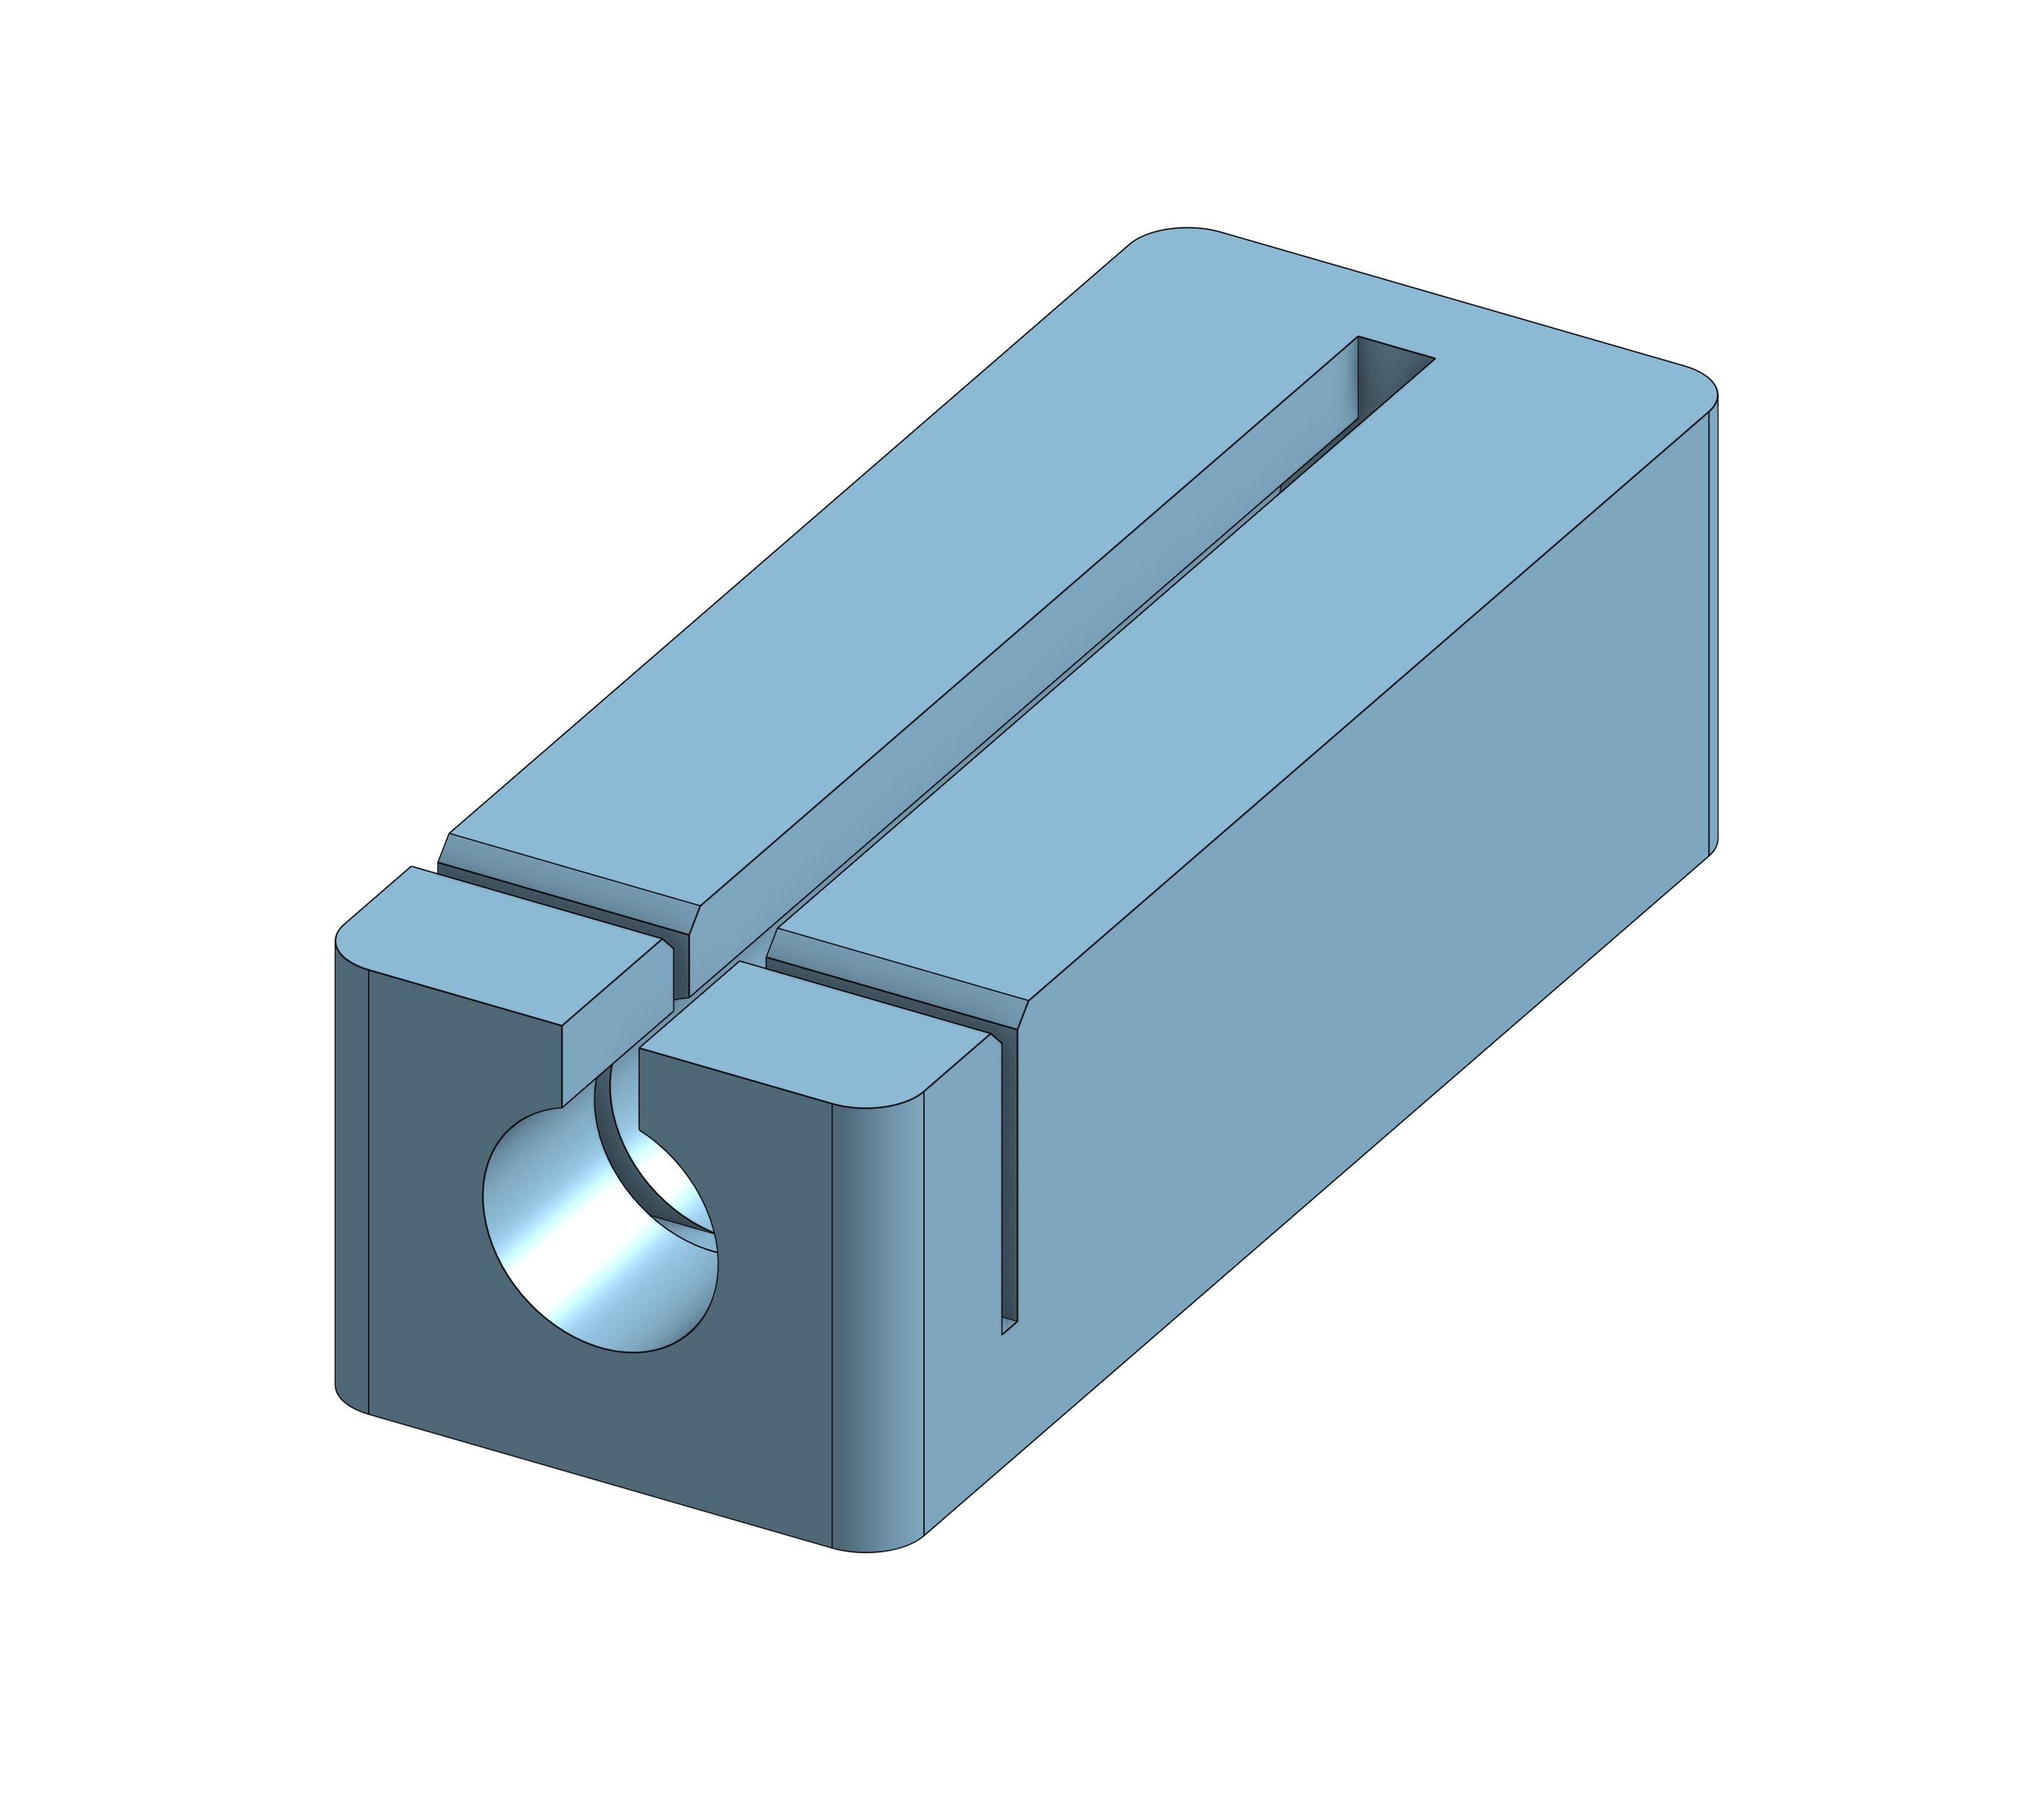
\includegraphics[width=.6\textwidth]{img/rod_cutting_tool.png}
   \caption{The Axle Cutting Tool.}
   \label{fig:C_T_RC} 
\end{figure}

\subsubsection*{Axle Drilling}

\textbf{Caution:} \textit{Carbon Fiber dust is not very nice to inhale, all carbon fiber related tasks that involve manufacturing should be done with the part submerged in water to prevent the dust getting in the air and in a well ventilated area with a respirator and eye protection.} \\

The rear axle interfaces with the other parts via M$2$ screws. This means that it needs a $\diameter 2$mm hole at each end. This hole is spaced $4.5$mm from each edge. To do this, a tool was needed. \\

The tool has a hole for a $2$mm High Speed Steel or Carbide Drill Bit and a hole for the tube to slot in till it hits an internal wall. It is printed with the back face, the only face without any features or fillets, pointing down (see Figure \ref{fig:C_T_RD}). It is printed at a layer height of $0.20$mm, has $3$ perimeters and a $25\%$ infill.

\begin{figure}[H]
   \centering
   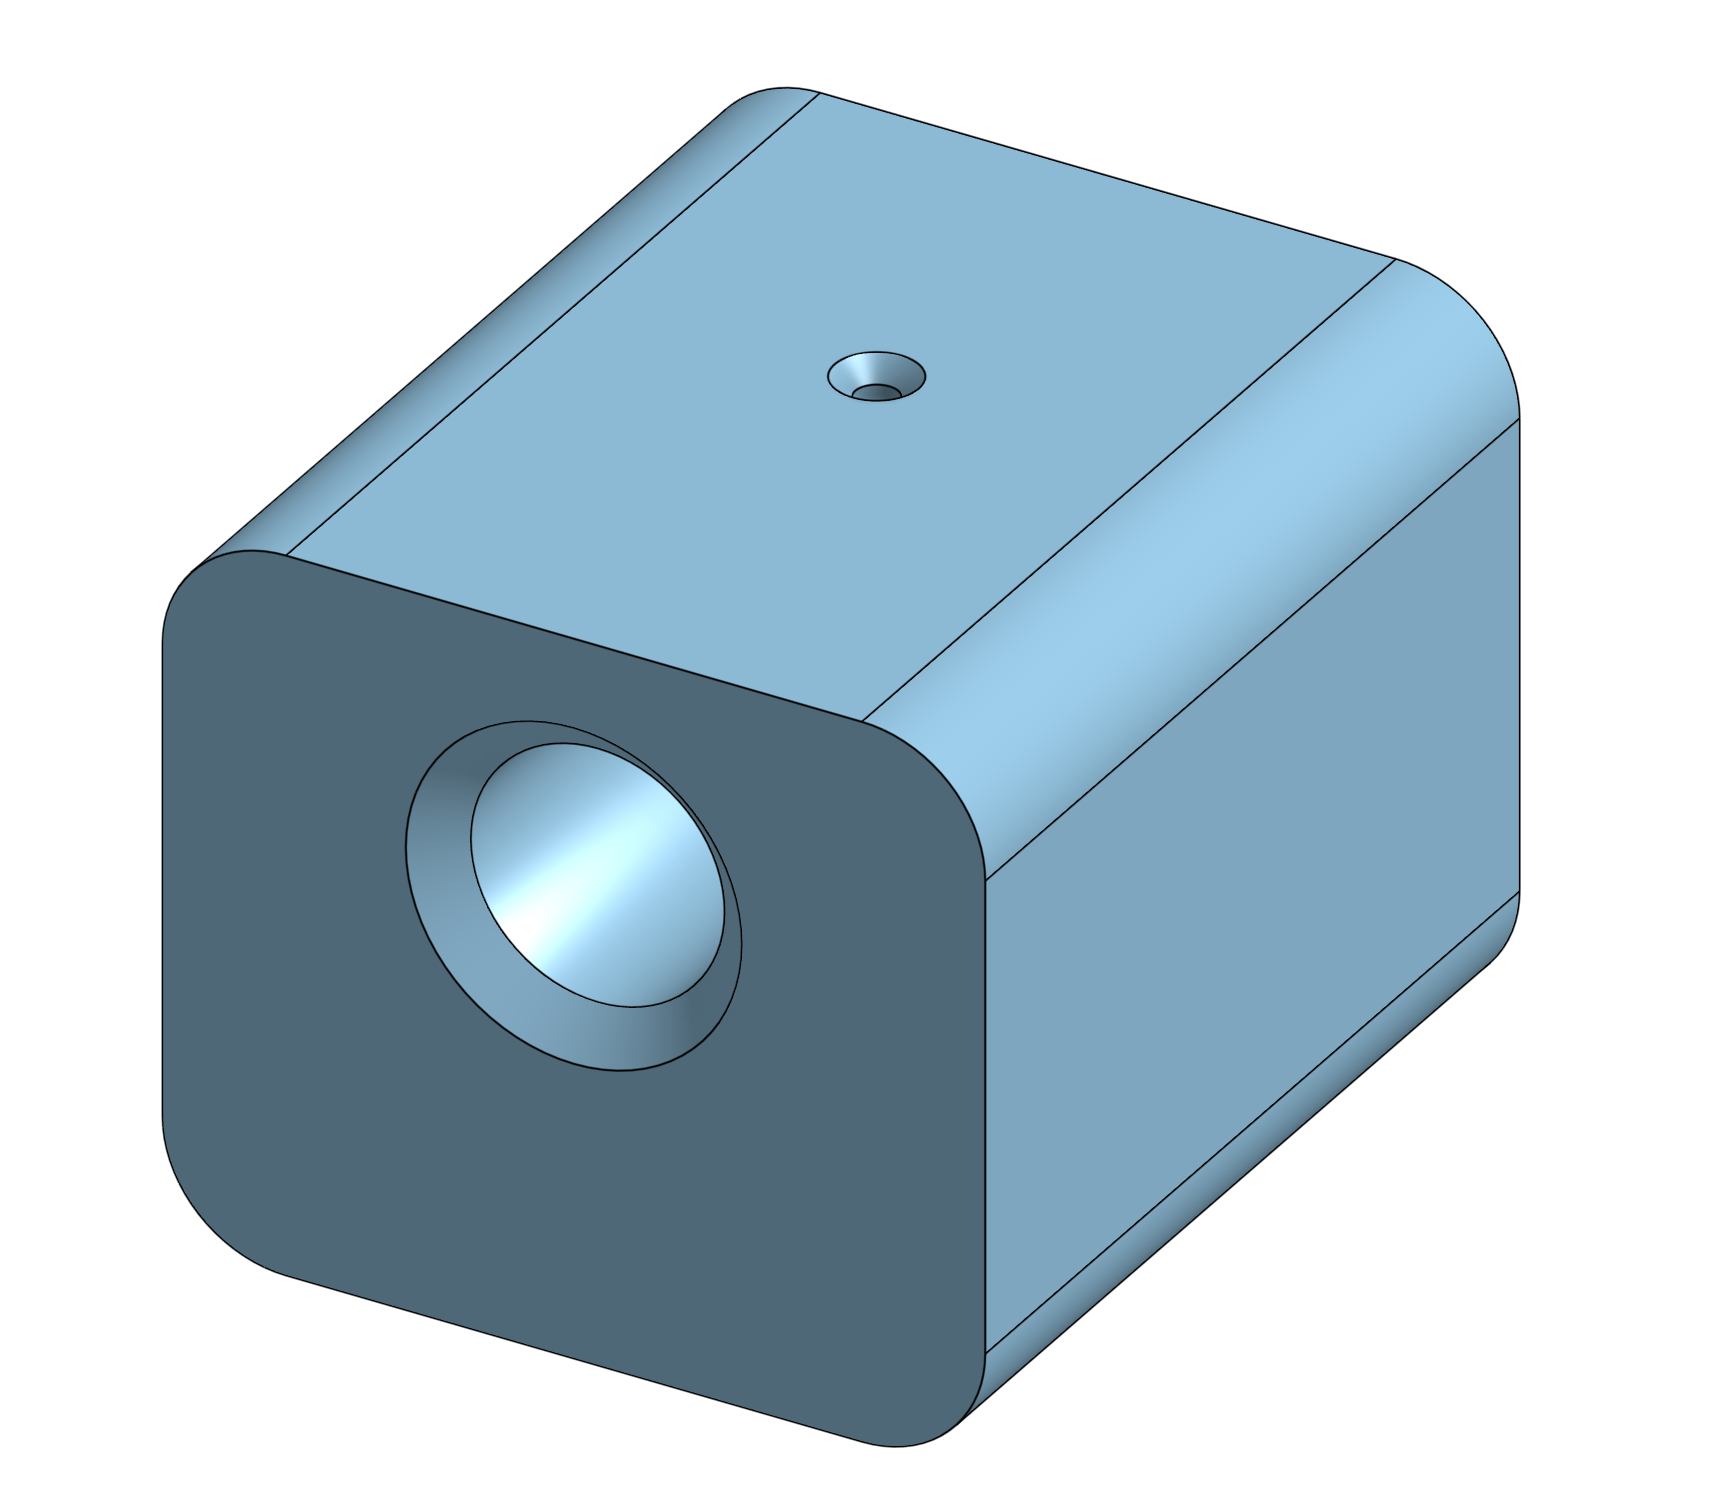
\includegraphics[width=.6\textwidth]{img/rod_drilling_tool.png}
   \caption{The Axle Drilling Tool.}
   \label{fig:C_T_RD} 
\end{figure}

\subsection{Notes}

All the parts are printed in PLA till mentioned otherwise.\\

The nominal settings are using the arachne wall engine with 3 bottom layers and 4 top layers with Gyroid infill. The nominal perimeter width is $0.4$mm. One may need some post processing if not using a well calibrated printer. Some parts intentionally do not have clearances to interact better. \\

All the $3$D files can be found in the "/models" directory, organized into sub sections. The files are in the ".STEP" format, allowing others to modify and change the files. The files are published under the GNU Affero General Public License (AGPL), meaning all changed files need to be published as well. \\

Thanks again to the Orca Slicer and the PreFlight Slicer teams for the amazing and open source software they provide. \\

\textbf{The BOM for the screws is available in the "other" as well as "models" folder.}



\pagebreak

\section{OS and Configurations}


The Raspberry Pi uses a $64$GB SD card. It is flashed with Ubuntu 22.04.5 Server. This is used with ROS 2 Humble Hawksbill. What is ROS and why use it?\\

ROS (Robot Operating System) is an open-source robotics middleware framework. Rather than a traditional operating system like Linux or Windows, ROS acts as a communication backbone. It connects the main compute board (e.g., Raspberry Pi) to your sensors (LiDAR, camera, IMU) and motor controllers, allowing different software modules to send data to each other seamlessly. \\

\textbf{Reasons to use ROS}
\begin{enumerate}
\item \textbf{Process Decoupling}: Runs perception, navigation, and motor control as separate, independent nodes. A crash or lag in image processing won't freeze the real-time steering/drive loop.
\item \textbf{Automated Frame Transformations (tf2)}: Computes precise spatial math and coordinate transforms between different physical points on the car (e.g., center of mass $\rightarrow$ LiDAR offset $\rightarrow$ camera offset).
\item \textbf{Sensor Synchronization}: Provides built-in tools (message filters) to align high-bandwidth feeds (camera frames and 2D LiDAR scans) with low-level IMU and encoder data.
\item \textbf{Data Logging \& Offline Replay (rosbag)}: Records full track run data to replay offline, letting you refine algorithms and tune controllers without physical track time or draining LiPo batteries.
\item \textbf{Live Visualization (RViz)}: Displays real-time 2D LiDAR sweeps, camera overlays, and projected path trajectories live on screen during testing.
\item \textbf{WRO Rubric Alignment}: Fulfills competition evaluation criteria for software modularity, state-machine design, and code reproducibility required in the engineering journal and GitHub repository (refer to README.md).
\end{enumerate}

Hence ROS was used. Why Humble Hawksbill? Because it was the latest stable release at the time of starting this. \\

\subsection{Camera ROS 2 Integration}

Ubuntu has a lot of driver issues, especially when running it on an SBC like a Raspberry Pi. They are annoying but navigable.

\subsubsection*{Driver Constraints \& Hardware Sensor Binning}
Configuring the Arducam IMX219 ($175^\circ$ FOV) on Ubuntu 22.04 LTS (64-bit) requires modern \texttt{libcamera} overlays rather than legacy MMAL drivers. To maintain the full field-of-view without cropping or high CPU overhead, the sensor's native \textbf{hardware binning (subsampling)} mode is utilized. This mode samples the entire $3280 \times 2464$ sensor plane but combines pixels on-chip down to $640 \times 480$, preserving the full $175^\circ$ FOV while drastically reducing transport latency for real-time ROS 2 inference.

\subsubsection*{Configuration \& Node Execution}
Configure the sensor overlay in \texttt{/boot/firmware/config.txt} (\texttt{start\_x=1}, \texttt{gpu\_mem=128}, \texttt{dtoverlay=imx219}) and reboot. 

After installing \texttt{ros-humble-camera-ros}, launch the camera node in binned $640 \times 480$ \texttt{RGB888} format to publish to  image/raw:
\begin{verbatim}
ros2 run camera_ros camera_node --ros-args \
  -p format:="RGB888" -p width:=640 -p height:=480
\end{verbatim}

\subsection{Hardware PWM Configuration \& Tuning}

\subsubsection*{Pinout \& Driver Setup}
Dual-channel hardware PWM on the Raspberry Pi 4B utilizes PWM0 (GPIO 12 / Pin 32) and PWM1 (GPIO 13 / Pin 33) operating at 50~Hz ($20\,\text{ms}$ period). Because the PWM hardware clock controller shares resources with onboard audio, audio must be disabled in firmware and blacklisted in the kernel:

\begin{enumerate}
    \item \textbf{Firmware Overlay:} Add \texttt{dtoverlay=pwm-2chan,pin=12,func=4,pin2=13,func2=4} and \texttt{dtparam=audio=off} to \texttt{/boot/firmware/config.txt}.
    \item \textbf{Kernel Blacklisting:} Blacklist the audio module by adding \texttt{blacklist snd\_bcm2835} to \texttt{/etc/modprobe.d/raspi-blacklist.conf}.
\end{enumerate}

\subsubsection*{Servo Pulse Limits \& Power Stability}
The S2500M steering servo is calibrated at 50~Hz with strict pulse boundaries:
\begin{itemize}
    \item \textbf{Pulse Boundaries:} Neutral at $1500\,\mu\text{s}$, minimum safe pulse at $700\,\mu\text{s}$ ($\approx 0^\circ$), and maximum safe pulse at $2300\,\mu\text{s}$ ($\approx 180^\circ$).
    \item \textbf{Thermal/Current Throttling:} Exceeding $2300\,\mu\text{s}$ forces the servo against mechanical hard stops, triggering internal thermal throttling with 5-second recovery delays.
    \item \textbf{Power Integrity:} Requires a common ground path across the Pi, HAT, and power rail, along with a $470\,\mu\text{F}$ decoupling capacitor across 5V/GND to absorb inrush spikes.
\end{itemize}

\subsubsection*{Linux Sysfs Execution Sequence}
When interfacing via \texttt{/sys/class/pwm/pwmchip0/}, write sysfs parameters in strict order:
\begin{enumerate}
    \item Disable output (\texttt{enable = 0}).
    \item Set period first (\texttt{period = 20000000}).
    \item Set pulse width second (\texttt{duty\_cycle = 1500000}).
    \item Enable output (\texttt{enable = 1}).
\end{enumerate}

\pagebreak

\section{Control Architecture \& Software System}

\subsection{System Architecture \& ROS 2 Pipeline}
The software stack is structured as a modular ROS 2 architecture comprising three primary subsystems: Perception, Decision \& Control, and Mobility/Actuation. Inter-node communication relies on standard ROS 2 topics to maintain real-time responsiveness.

\begin{figure}[h!]
\centering
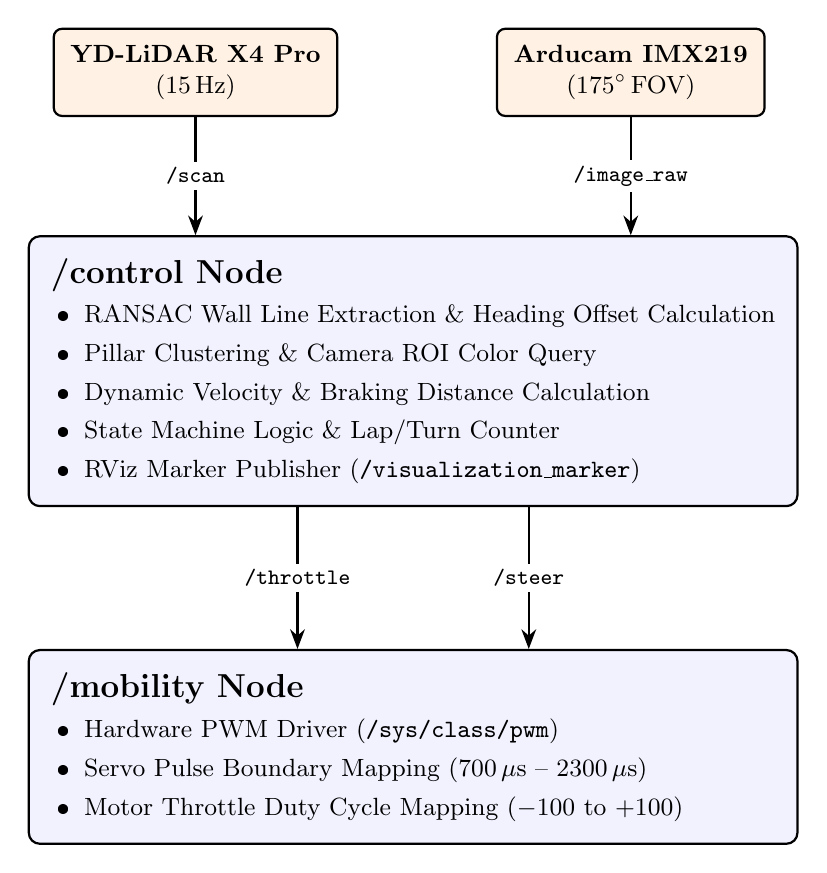
\begin{tikzpicture}[
    node distance = 1.2cm and 1.5cm,
    sensor/.style = {rectangle, draw, rounded corners=3pt, fill=orange!10, thick, align=center, inner sep=6pt, font=\small},
    nodeblock/.style = {rectangle, draw, rounded corners=4pt, fill=blue!5, thick, align=left, inner sep=8pt, font=\small},
    arrow/.style = {-{Stealth[length=2.5mm]}, thick},
    topicalign/.style = {font=\footnotesize\ttfamily, fill=white, inner sep=2pt}
]

    % Sensor Nodes
    \node (lidar) [sensor] {\textbf{YD-LiDAR X4 Pro}\\(15\,Hz)};
    \node (camera) [sensor, right=2.0cm of lidar] {\textbf{Arducam IMX219}\\($175^\circ$\,FOV)};

    % Decision / Control Node
    \node (control) [nodeblock, below=1.5cm of $(lidar.south)!0.5!(camera.south)$, anchor=north] {
        \textbf{\large /control Node}\\[4pt]
        \begin{minipage}{9.2cm}
        \begin{itemize}[leftmargin=12pt, itemsep=1pt, topsep=2pt]
            \item RANSAC Wall Line Extraction \& Heading Offset Calculation
            \item Pillar Clustering \& Camera ROI Color Query
            \item Dynamic Velocity \& Braking Distance Calculation
            \item State Machine Logic \& Lap/Turn Counter
            \item RViz Marker Publisher (\texttt{/visualization\_marker})
        \end{itemize}
        \end{minipage}
    };

    % Mobility / Actuation Node
    \node (mobility) [nodeblock, below=1.8cm of control.south, anchor=north] {
        \textbf{\large /mobility Node}\\[4pt]
        \begin{minipage}{9.2cm}
        \begin{itemize}[leftmargin=12pt, itemsep=1pt, topsep=2pt]
            \item Hardware PWM Driver (\texttt{/sys/class/pwm})
            \item Servo Pulse Boundary Mapping ($700\,\mu\text{s}$ -- $2300\,\mu\text{s}$)
            \item Motor Throttle Duty Cycle Mapping ($-100$ to $+100$)
        \end{itemize}
        \end{minipage}
    };

    % Sensor Dataflow Arrows
    \draw [arrow] (lidar.south) -- (lidar.south |- control.north) 
        node[midway, topicalign] {/scan};
    \draw [arrow] (camera.south) -- (camera.south |- control.north) 
        node[midway, topicalign] {/image\_raw};

    % Mobility Control Arrows
    \draw [arrow] ($(control.south)!0.3!(control.south west)$) -- ($(mobility.north)!0.3!(mobility.north west)$) 
        node[midway, topicalign] {/throttle};
    \draw [arrow] ($(control.south)!0.3!(control.south east)$) -- ($(mobility.north)!0.3!(mobility.north east)$) 
        node[midway, topicalign] {/steer};

\end{tikzpicture}
\caption{ROS 2 System Control Architecture and Inter-Node Dataflow Diagram.}
\label{fig:control_architecture}
\end{figure}

\subsection{ROS 2 Topics \& Interfaces}
\begin{itemize}
    \item \textbf{\texttt{/scan} Topic (\texttt{sensor\_msgs/msg/LaserScan}):} Published by the LiDAR node at a nominal frequency of $15\,\text{Hz}$, containing 2D range arrays over $360^\circ$.
    \item \textbf{\texttt{/steer} Topic (\texttt{std\_msgs/msg/Float32}):} Published by the \texttt{/control} node to command target Ackermann steering angles. The \texttt{/mobility} node maps these commands to PWM duty cycles ($700\,\mu\text{s}$ to $2300\,\mu\text{s}$) on GPIO 12.
    \item \textbf{\texttt{/throttle} Topic (\texttt{std\_msgs/msg/Int8}):} Published by the \texttt{/control} node to set motor velocity demands from $-100$ (full braking / reverse) to $+100$ (maximum forward acceleration), with $0$ representing neutral.
    \item \textbf{\texttt{/visualization\_marker} Topic (\texttt{visualization\_msgs/msg/Marker}):} Streams 3D geometric markers to RViz to display vehicle position, extracted wall vectors, and mapped pillar locations.
\end{itemize}

\subsection{Perception Algorithms \& Path Extraction}

\subsubsection{RANSAC Wall Extraction \& Heading Offset}
2D range arrays from \texttt{/scan} within the perception radius are processed using a Random Sample Consensus (RANSAC) line-fitting algorithm to extract straight wall vectors. The controller calculates the lateral offset error $e_d$ and heading angular error $\theta$ relative to the wall vector to derive the Ackermann steering command $\delta$:
\begin{equation}
\delta = K_p \cdot \theta + K_d \cdot e_d
\end{equation}
where $K_p$ and $K_d$ represent proportional and derivative control gains.

\subsubsection{Dynamic Velocity-Dependent Braking}
To prevent cornering overshoot, the braking initiation distance $d_{\text{brake}}$ is calculated dynamically as a function of current vehicle velocity $v$:
\begin{equation}
d_{\text{brake}} = d_{\text{min}} + k_v \cdot v^2
\end{equation}
where $d_{\text{min}}$ is the baseline stopping distance and $k_v$ is an empirical braking coefficient.

\subsection{Challenge Execution Logic}

\subsubsection{Round One: Obstacle-Free Wall Following}
\paragraph{Startup Sequence:} Pressing the hardware start switch initiates a non-blocking startup delay. This allows the LiDAR motor to reach nominal operating speed ($15\,\text{Hz}$) and ensures team members clear the operational area.

\paragraph{Wall-Following \& Turn Management:} The \texttt{/control} node evaluates wall vectors to execute directional turns, adjusts dynamic velocity/braking thresholds, and tracks completed turns and laps.

\subsubsection{Round Two: Pillar Mapping \& Parallel Parking}
\paragraph{Exit Maneuver \& Direction Initialization:} Operation begins with an automated exit sequence from the parallel parking bay, after which the primary circuit direction is established.

\paragraph{Pillar Clustering \& Camera Color Fusion:} The \texttt{/control} node clusters contiguous points in \texttt{/scan} data to detect cylindrical pillars, computing their range and bearing angle $\phi$. The node queries the wide-angle camera for average color values (RGB/HSV) within the Region of Interest (ROI) corresponding to bearing $\phi$. The identified color (Red/Green) is logged on the occupancy map to dictate navigation paths (e.g., passing Red pillars on the right, Green on the left).

\paragraph{Automated Parallel Parking Finalization:} Upon completing the pillar circuit, the vehicle transitions into parallel parking mode, utilizing lateral wall range measurements to execute a multi-point alignment into the parking bay.

\pagebreak

\section{Conclusion \& Acknowledgments}

Building our autonomous vehicle for the WRO Future Engineers challenge has been an invaluable journey of iterative design, engineering trade-offs, and practical problem-solving. From casting custom $40\text{A}$ polyurethane tires and designing a 4-layer PCB hat to configuring ROS 2 nodes and tuning hardware PWM timings, every sub-assembly represents hands-on learning and technical growth.

\subsection{Document Production}
This manual and technical documentation suite were authored using \LaTeX{} and compiled using \textbf{TeXmaker}. In the spirit of open collaboration, all CAD STEP models, schematics, and hardware BOMs are published under the GNU Affero General Public License (AGPLv3) for the robotics community.

\subsection{Open-Source Acknowledgments}
This project relies heavily on the open-source ecosystem and accessible software platforms. We express our gratitude to the developers, maintainers, and communities behind the following tools:

\begin{itemize}
    \item \textbf{TeXmaker \& \LaTeX{}:} For providing a reliable typesetting environment for technical manual generation.
    \item \textbf{KiCAD:} For enabling 4-layer PCB schematic capture, routing, and 3D visualization.
    \item \textbf{Orca Slicer \& PreFlight Slicer:} For advanced toolpath generation, Arachne wall engines, and precise 3D printing execution.
    \item \textbf{ROS 2 (Humble Hawksbill):} For supplying a robust middleware framework for robotics perception and node communication.
    \item \textbf{Onshape:} For flexible 3D CAD modeling and parametric assembly management.
    \item \textbf{Interactive HTML BOM:} For generating interactive assembly guides for surface-mount soldering.
    \item \textbf{Linux \& Raspberry Pi Community:} For maintaining the embedded drivers, overlays, and hardware documentation.
\end{itemize}

Thank you to the WRO organizers, judges, fellow competitors, and the broader open-source community for making this journey possible.

\end{document}